\documentclass[letterpaper,11pt]{memoir}
\usepackage[margin=2.5cm,includehead,includefoot,footskip=30pt]{geometry}
\usepackage{lmodern}
\usepackage{titletoc}
\usepackage{cite}
\usepackage{amsmath}
\usepackage{graphicx}
\usepackage{float}
\usepackage{xcolor}
% \usepackage{showkeys}

\changecaptionwidth
\captionwidth{0.8\textwidth}

\maxtocdepth{subsection}
\setsecnumdepth{subsubsection}
\setpnumwidth{3em}

\definecolor{blue}{rgb}{0.149,0.545,0.824}
\definecolor{red}{rgb}{0.647,0.129,0.149}

\renewcommand\colorchapnum{\color{red}}
\chapterstyle{hangnum}
\renewcommand*{\chapnamefont}{\normalfont\Huge\scshape}
\renewcommand*{\chapnumfont}{\normalfont\fontsize{50}{60}\slshape\colorchapnum}
\renewcommand*{\chaptitlefont}{\normalfont\HUGE\scshape\colorchaptitle}

\newcommand{\partialtoc}{
\vspace*{2pc}\vbox{\bfseries\Large Outline}\vspace*{5pt}\hrule\vspace*{1pc}%
\startcontents[chapters]
\printcontents[chapters]{}{1}{\setcounter{tocdepth}{3}}
\vspace*{1pc}\hrule\vspace*{2pc}}

\usepackage[bookmarksdepth=2,colorlinks=true,linkcolor=blue,
            citecolor=red,filecolor=magenta,urlcolor=blue,
            breaklinks=true]{hyperref}
\urlstyle{same}
\hypersetup{% PDF display options
   pdftitle={Theoretical Optical Second-Harmonic Calculations for Surfaces},
   pdfauthor={Sean M. Anderson},
   pdfsubject={Theory of SSHG in crystalline semiconductors, from the nonlinear
   polarization and susceptility, to the SSHG radiation with results.},
   pdfkeywords={nonlinear} {optics} {shg} {radiation} {semiconductors}
   {theoretical} {spectroscopy} {surface} {experiment}}

\newsubfloat{figure}

\begin{document}

\frontmatter
\renewcommand{\thepage}{\Roman{page}}
%!TEX root = ../../main.tex
\begin{titlingpage}
\begin{center}
\vspace*{2cm}
{\Huge Optimized Software for Theoretical Nonlinear Optical Calculations}
\vspace{1.0cm}

{\large by}
\vspace{1.0cm}

{\LARGE \href{mailto:sean.martin.anderson@gmail.com}{Sean M. Anderson}}
\vspace{3cm}

{\Large A thesis submitted in partial fulfillment of the requirements\\
\vspace{0.25cm}
for the degree of Doctor of Philosophy.}
\vspace{4cm}

{\large Advisor:\\
Dr. Bernardo S. Mendoza
\vspace*{1cm}

Divisi\'on de Fot\'onica\\
Centro de Investigaciones en \'Optica, A.C.\\
Loma del Bosque 115, Le\'on, Guanajuato, 37150, M\'exico}
\vfill
\today
\end{center}
\end{titlingpage}

\null
\vfill
\begin{flushleft}
The research presented in this thesis was carried out at the Centro de
Investigaciones en \'Optica, A.C., Loma del Bosque 115, Le\'on, Guanajuato,
37150, Mexico, in collaboration with the Laboratoire des Solides Irradi\'es,
\'Ecole Polytechnique, CNRS, CEA/DSM, 91128 Palaiseau, France, which is a part
of the European Theoretical Spectroscopy Facility (ETSF), Palaiseau, France.
Funding was provided by the CONACyT (Consejo Nacional de Ciencia y Tecnolog\'ia)
in Mexico, through scholarship N\textsuperscript{o} 349278.

\vspace{1cm}

Copyright {\copyright{}} 2016 by 
\href{mailto:sean.martin.anderson@gmail.com}{Sean M. Anderson}.
\end{flushleft}

\clearpage

%!TEX root = ../../main.tex
\begin{titlingpage}

\begin{center}
    \vspace*{1cm}
    {\LARGE Optimized Software for Theoretical Optical Calculations}\\
    \vspace{0.7cm}
    {\large by}\\
    \vspace{0.7cm}
    {\Large Sean M. Anderson}
\end{center}

\vfill
{\Large Approved:}

\begin{flushright}

\vspace*{1cm}

\makebox[0.5\textwidth ]{\hrulefill}\\
\textbf{Dr. Bernardo Mendoza Santoyo}\\ Thesis Advisor
\vspace{1.25cm}

\makebox[0.5\textwidth ]{\hrulefill}\\
\textbf{Dr. Wolf Luis Moch\'an Bacal}\\ External Reader
\vspace{1.25cm}

\makebox[0.5\textwidth ]{\hrulefill}\\
\textbf{Dr. Ram\'on Carriles Jaimes}\\ Reader
\vfill

\end{flushright}

\begin{center}
    {\large 
    Centro de Investigaciones en \'Optica, A.C.\\
    Loma del Bosque 115, Le\'on, Guanajuato, 37150, M\'exico\\
    \today
    }
\end{center}

\end{titlingpage}

%!TEX root = ../../main.tex
\begin{titlingpage}

\null
\vfill

\begin{flushright}
{\huge \emph{``The purpose of computing is insight, not numbers.''}}\\
% \rule{0.85\textwidth}{1pt}

\vspace{10pt}

{\LARGE Richard Hamming}
\end{flushright}

\vfill
\end{titlingpage}

\pagestyle{plain}
\begin{vcenterpage}
{\LARGE{\sc Abstract}}

\noindent\rule[2pt]{\textwidth}{0.5pt}
Lorem ipsum dolor sit amet, consectetur adipiscing elit. Sed libero elit, sollicitudin dignissim accumsan aliquam, eleifend et massa. Suspendisse porta luctus metus, vitae pellentesque ante porttitor ut. Etiam id magna sit amet metus dignissim imperdiet eget a enim. Lorem ipsum dolor sit amet, consectetur adipiscing elit. In placerat, nunc ut volutpat aliquet, nunc sem blandit dui, nec hendrerit justo augue non mauris. Donec non enim in nibh rutrum mollis a sit amet nisl. Praesent augue lacus, eleifend at malesuada eget, rutrum ut est. Suspendisse at arcu nunc. Donec congue pretium nisi ac sodales. Duis aliquam urna eget elit luctus ut feugiat diam lacinia. Quisque libero mi, gravida a elementum non, dictum vitae lorem.

Nullam purus ipsum, dapibus eget rhoncus eu, aliquet id felis. Phasellus ultrices, dolor sed sollicitudin interdum, diam mi consequat magna, at feugiat nisl quam in purus. Nulla mauris augue, hendrerit eu malesuada sit amet, ornare et est. Sed pulvinar justo sit amet dui accumsan fringilla. Praesent augue est, sagittis bibendum posuere sit amet, sodales id mauris. Nulla dapibus eleifend malesuada. Maecenas consequat eleifend sem, et dapibus erat cursus a.

\noindent\rule[2pt]{\textwidth}{0.5pt}
\end{vcenterpage}

\begin{vcenterpage}
{\LARGE{\sc Dedication}}

\noindent\rule[2pt]{\textwidth}{0.5pt}

Lorem ipsum dolor sit amet, consectetur adipiscing elit. Sed libero elit, sollicitudin dignissim accumsan aliquam, eleifend et massa. 

\noindent\rule[2pt]{\textwidth}{0.5pt}
\end{vcenterpage}

\begin{vcenterpage}
{\LARGE{\sc Acknowledgements}}

\noindent\rule[2pt]{\textwidth}{0.5pt}

Lorem ipsum dolor sit amet, consectetur adipiscing elit. Sed libero elit, sollicitudin dignissim accumsan aliquam, eleifend et massa. Suspendisse porta luctus metus, vitae pellentesque ante porttitor ut. Etiam id magna sit amet metus dignissim imperdiet eget a enim. Lorem ipsum dolor sit amet, consectetur adipiscing elit. In placerat, nunc ut volutpat aliquet, nunc sem blandit dui, nec hendrerit justo augue non mauris. Donec non enim in nibh rutrum mollis a sit amet nisl. Praesent augue lacus, eleifend at malesuada eget, rutrum ut est. Suspendisse at arcu nunc. Donec congue pretium nisi ac sodales. Duis aliquam urna eget elit luctus ut feugiat diam lacinia. Quisque libero mi, gravida a elementum non, dictum vitae lorem.

Nullam purus ipsum, dapibus eget rhoncus eu, aliquet id felis. Phasellus ultrices, dolor sed sollicitudin interdum, diam mi consequat magna, at feugiat nisl quam in purus. Nulla mauris augue, hendrerit eu malesuada sit amet, ornare et est. Sed pulvinar justo sit amet dui accumsan fringilla. Praesent augue est, sagittis bibendum posuere sit amet, sodales id mauris. Nulla dapibus eleifend malesuada. Maecenas consequat eleifend sem, et dapibus erat cursus a.

Donec metus magna, laoreet tempor hendrerit ut, volutpat at augue. Vivamus at vestibulum nisl. Donec elit augue, pulvinar ac rhoncus vitae, euismod tristique quam. Etiam in nisl justo. Phasellus eu sem sed purus lacinia rutrum id sed lorem. Cras neque tortor, rutrum ut pulvinar eget, vehicula eget lacus. Etiam pretium metus metus.

Vivamus velit nulla, ultrices a ultrices vel, rhoncus nec dui. Praesent accumsan libero eu tellus feugiat sodales. Donec et quam a diam eleifend ultricies semper nec justo. Cras euismod fermentum tellus, vitae tincidunt enim sodales id. Proin ultrices tellus at felis imperdiet nec tempor diam accumsan. Curabitur et posuere magna. Phasellus ultricies, orci vel mattis adipiscing, nulla elit semper odio, id sollicitudin purus sapien a ligula. Proin porta hendrerit justo quis venenatis. Integer et iaculis urna. Nulla ut justo ante.

\noindent\rule[2pt]{\textwidth}{0.5pt}
\end{vcenterpage}

\tableofcontents*\clearpage
\listoffigures*\clearpage
\listoftables*

\mainmatter
\pagestyle{ruled}
%!TEX root = ../../main.tex
\chapter{Introduction}\label{ch:intro}
\minitoc

\section{Motivation}
The principal motivation for this work is the analysis of different nanoparticles following two concepts:

\begin{description}
\item[First,] the use of second-order nonlinear optical effects that are very effective for surface analysis.
\item[Second,] the use of a special technique for optical spectroscopy -- the two beam, cross-polarized second harmonic/sum-frequency generation (XP2SHG/ SFG) technique. 
\end{description}

Metallic nanoparticles are currently a ``hot topic'' in the scientific world because the scope of their potential applications is very large, from biological applications \cite{baroli2007penetration}, imaging and detection \cite{lindfors2004detection, haick2007chemical, berciaud2006photothermal}, and more \cite{kamyshny2005ink, krenn1999squeezing}. Silicon nanoparticles, although more common, are not far behind -- their use in new solar cell technologies \cite{pillai2007surface} and biological markers \cite{li2004water} are also cutting edge research. 

None of the techniques described in this thesis are particularly new, but they have been used with great success in a variety of different materials. Although some literature exists on metallic nanoparticles characterized by these techniques, there is a relatively small amount of research on the subject. The optical methods included here are both non-destructive and potentially surface specific. Combining these with interesting nanostructures may prove to be a promising path for future developments in the nanosciences.

The focus of this thesis will be the study of second-order nonlinear effects in nanosystems. Nanoparticles have huge surface to volume ratios because they are so small; they contain few atoms and the bulk is tiny compared to the outside surface. The second-order nonlinearities, second harmonic generation (SHG) and sum-frequency generation (SFG), are both suitable for spectroscopic analysis of nanoparticles. These can be greatly enhanced using the two beam, cross-polarized SHG/SFG (XP2SHG/SFG) technique \cite{figliozzi2005single}. The purpose of this work is to study the properties of these nanostructures using the aforementioned methods.

\section{Nonlinear Optics in a Nutshell}\label{chap_intro_nonlin}
Linear optics has long dominated the study of light. Much like Newton's mechanics, it describes an incomplete picture of the interaction between light and the matter that forms our world. This is not to say the picture is incorrect; the interactions described work for our everyday situations. We call them ``linear'' because matter interacts in a directly proportional way with the electric field of the incoming light. The linear response of most materials is more appreciable than the other responses, making them difficult to observe -- we call these ``nonlinear effects.'' We will elaborate further on this point in chapter \ref{chap_theory}.

We can approximate most potentials within the atom using a harmonic oscillator model. These potentials represent the effect electrons feel when confined. They restrict the way electrons can move and determine many of the important material properties. These can tell us whether a material would make a good semiconductor for an optical device or for a computer microprocessor, or would make a very conductive metal, amongst many other things.

An example of a harmonic oscillator is a spring with a mass on one end. The other end is fixed and unmovable. If the mass is moved a little ways away from the equilibrium point and released, the mass will begin to oscillate for some time until it eventually stops once again at equilibrium (as it is dampened by gravity or friction). However, if you pull the spring too far it can deform from all the extra force. The spring follows a linear response according to the well established SHO equations when the displacement is small. Larger displacements are unaccounted for in this model -- now we are talking about \emph{nonlinear} behavior.

So the electrons behave in a similar manner if we model our electronic potentials as SHOs. This model works well for low intensities of incoming light, when the electron is displaced only a little from the ``bottom'' of the potential well. This provides the linear response between light and matter and is the reason why linear interactions dominate our everyday life. Although the light is very intense, the radiation that does reach us is spread out over half our world. Even when focused down to a very bright point it lacks the ability to deliver energy in an organized and efficient way. So our everyday light can only give electrons a little bit of energy and they move accordingly. Even the sun cannot provide the necessary conditions to allow electrons to move significantly from the bottom of a potential well.

We had the sun and different light bulbs, and used them often for experiments. I just explained why these sources can't help us past the linear regime. So people were stuck with this problem for a long time until a new light source, the LASER, was invented. LASER is an acronym for \emph{Light Amplification by Stimulated Emission of Radiation}. One of the main characteristics of a laser is that it emits an energetic, unidirectional, coherent beam of light that can be focused to a very small spot further concentrating the energy.

This discovery revolutionized optical science. The laser was precisely what was needed to produce high energy densities that could move the electrons away from the bottom of the potential well. Experimentalists starting shooting lasers into all kinds of materials -- and just like the spring and mass, the model stopped describing the experiment and all sorts of strange things started happening.

In this way we discovered nonlinear optics. These strange effects were difficult to explain at first. A new model had to be devised and tested against the experiments. Fortunately, it was not very long before one was created and found to work; not only did it explain everything observed until then, but it also predicted many things that had not yet been discovered \cite{boyd2003nonlinear, diels2006ultrashort, shen1984principles}. I will elaborate on the math of this new model in chapter.

SHG, a special case of SFG, was one of the first observed, and predominant optical nonlinearities that can appear from many substances. While all materials are technically nonlinear, the response of most are not appreciable for low intensities of incoming light, and are destroyed before we can see the effects. Some metals and semiconductors are excellent nonlinear materials, as are many different crystals. SHG is usually the first nonlinear effect to appear and can be the easiest to produce. As we will explain in section , it is often attributed to surface emission which makes it an excellent tool for studying and characterizing surfaces and interfaces.

\section{Outline}
This thesis is divided into 5 chapters including this introduction. Chapter  details the mathematics, formalism, and theory that make up our description of nonlinear optics. Chapter describes the materials to be characterized and the experimental setup used to study them. Chapter consists of the experimental data and analysis, with comparisons to existing literature. Finally, chapter  is dedicated to the final observations and remarks. The complete bibliography is located at the end of the document for easy reference.

\section{A Review of Nonlinear Optics}
\subsection{Historical Overview}\label{chap_theory_hist}
The discovery of the optical maser by Townes \cite{PhysRev.112.1940} and the construction of the laser by Maiman in the late 1950s and early 1960s ushered a new age of optical discoveries. The ability to produce optical beams with these devices automatically lead to very highly focused energies distributed over very small areas. These concentrated energies allowed scientists to finally move into the optical nonlinear regime for many different materials.

The optical maser allowed for the first recorded observation of optical SHG by Franken et al. in 1961 \cite{PhysRevLett.7.118}. They produced a second beam of light at twice the frequency of the original by exciting a piece of crystalline quartz. This frequency doubling effect was dubbed SHG and was observed to be much less intense than the exciting beam.

There is a humorous anecdote about this experiment. Apparently, the editor of Physical Review Letters thought that the second harmonic dot on the photographic plate was a speck of dust, which he edited out. The image found in the article has an arrow pointing at the empty spot where it should be. However, this did not detract from the importance of the find.

Other developments followed promptly. In 1962, Bloembergen et al. \cite{PhysRev.127.1918, PhysRev.128.606} developed the mathematical framework to explain nonlinear optical phenomena. That same year, Terhune et al. \cite{PhysRevLett.8.404} observed SHG in calcite. These discoveries were amongst others \cite{lax1962nonlinear} that lead to further research into the geometrical dependence of nonlinear effects, and helped verify that the majority of the SHG signal produced in a centrosymmetric material comes from surface contribution, where inversion symmetry is broken.

In the late 1960s, Bloembergen \cite{PhysRev.174.813} and others \cite{PhysRev.178.1218} studied SHG in a variety of centrosymmetric materials and semiconductors. The advent of pulsed lasers during the 1970s \cite{nla.cat-vn2583352} allowed for even greater intensities to be obtained. Dye lasers came to prominence during these years, offering very large bandwidths and relatively short picosecond pulses. However, these lasers were very difficult to maintain and the dyes used were typically very toxic and presented serious health risks.

Interest began to form around using SHG to study surfaces and interfaces, since it had been proven \cite{PhysRevLett.46.145} to be exclusive to the surface area of a centrosymmetric material in the dipole approximation. Shen et al. published \cite{PhysRevB.38.7985} that there is also a quadrupole bulk contribution for this kind of material, and in 1989 \cite{shen89nature} published a review article summarizing most of the trends in surface spectroscopy using SHG. Theoretical work also played an important role in the 1990s, with new theoretical models by Sipe \cite{PhysRevB.53.10751} and others \cite{PhysRevB.53.4999, PhysRevB.60.14334, PhysRevB.55.2489, PhysRevB.57.2569}. Downer et al. \cite{downer2001optical} and L\"upke \cite{Lupke199975} both produced very thorough and referenced texts on SHG surface spectroscopy of semiconductors in the late 1990s and early 2000s. This period of time provided the foundations for surface optics today.

At around the same time, the first Ti:sapphire lasers were being produced and analyzed \cite{Moulton:86}. These early ultrafast lasers were capable of producing femtosecond pulses via mode-locked oscillators. Since the active medium is in solid state form, they present none of the risks of using dyes. These lasers were considerably more compact than dye lasers since they no longer needed external dye control systems. These lasers became commercial in the early 1990s.

Chirped pulse amplification (CPA) was invented in 1985 by Mourou and Strickland \cite{Strickland1985447}. This technique allowed Ti:sapphire lasers to achieve much higher peak energy without compromising the ultrashort pulse duration. During the 1990s, CPA became the prominent method for increasing energy output in Ti:sapphire lasers. At this point, Ti:sapphire lasers using the CPA technique were both compact, efficient, and cost effective. These factors would only improve over the following decade as the Ti:sapphire laser became the standard for high energy, ultrashort pulse applications.

\subsection{Defintion of Nonlinear Optics}
As explained briefly in section \ref{chap_intro_nonlin}, linear optics predominate in our everyday lives. The intensity of the light sources that surround us is typically not sufficient to modify the optical properties of a material. The discovery of the laser gave us access to higher intensity of polarized, directional, and coherent light. Beyond this, the ultrafast pulsed laser provides energy distributed into a much shorter time-frame which increases the peak irradiance delivered. These advances have greatly reduced the cost and effort needed to study nonlinear phenomena.

Light is nothing more than electromagnetic radiation, and is therefore composed of electromagnetic fields. This means that the study of how matter interacts with light is merely the study of how the light fields interact with the structure of matter. This can be readily appreciated for crystals and materials with very organized structures -- in fact, the best nonlinear materials are almost always crystalline in nature.

\subsubsection{Nonlinear Polarization and Susceptibility}
So what happens when very intense light coincides on a given material? Let us talk about the dipole moment per unit volume, or polarization $\mathbf{P}(t)$. This polarization describes the effect light has on a material and vice versa; it represents the optical response of a material.Taking Maxwell's equations with the usual considerations of zero charge density ($\rho=0$) and no free currents ($\mathbf{J}=0$), we have

\begin{align}
\nabla\cdot\mathbf{D} &= 0,\label{eq_max_1}\\
\nabla\cdot\mu_{0}\mathbf{H} &= 0,\\
\nabla\times\mathbf{E} &= -\mu_{0}\frac{\partial\mathbf{H}}{\partial t},\\
\nabla\times\mathbf{H} &= \frac{\partial\mathbf{D}}{\partial t}.
\end{align}

We take into account the nonlinearity of the material by relating the \textbf{D} and \textbf{E} fields with the total (linear and nonlinear) polarization \textbf{P},

\begin{equation}
\mathbf{D} = \epsilon_{0}\mathbf{E} + \mathbf{P}.
\end{equation}

Proceeding in the usual manner for deriving the wave equation, we obtain
\begin{equation}
\nabla\times\nabla\times\mathbf{E} + \frac{1}{c^{2}}\frac{\partial^{2}}{\partial t^{2}}\mathbf{E} = -\frac{1}{\epsilon_{0}c^{2}}\frac{\partial^{2}\mathbf{P}}{\partial t^{2}},
\end{equation}

which can be considerably simplified thanks to the identity
\begin{equation}
\nabla\times\nabla\times\mathbf{E} = \nabla\left(\nabla\cdot\mathbf{E}\right)-\nabla^{2}\mathbf{E}.
\end{equation}

The $\nabla\left(\nabla\cdot\mathbf{E}\right)$ term is usually negligible (for instance, if $\mathbf{E}$ is of the form of a transverse, infinite plane wave), so we can finally express the inhomogenous wave equation as
\begin{equation}
\nabla^{2}\mathbf{E} - \frac{1}{c^{2}}\frac{\partial^{2}}{\partial t^{2}}\mathbf{E} = \frac{1}{\epsilon_{0}c^{2}}\frac{\partial^{2}\mathbf{P}}{\partial t^{2}}.
\end{equation}

In this form, it is clear that the polarization acts as a source for this differential equation and we can recall our oscillator example from section \ref{chap_intro_nonlin}. The polarization can be expressed by a power series of the form
\begin{align}
{P}(t) &= \epsilon_{0}\left[\chi^{(1)}{E}(t) + \chi^{(2)}{E}^{2}(t) + \chi^{(3)}{E}^{3}(t) + \ldots\right]\label{eq_power}\\
             &\equiv {P}^{(1)}(t) + {P}^{(2)}(t) + {P}^{(3)}(t) + \ldots,\label{eq_p_series}
\end{align}

where $\chi^{(n)}$ is the n\textsuperscript{th}-order susceptibility of the material. We can define the susceptibility as a constant of proportionallity that describes the degree of polarizability a material has in terms of the strength of an incoming optical electric field. The first term
\begin{equation}
P(t) = \epsilon_{0}\chi^{(1)}E(t),
\end{equation}

is the linear term that describes most everyday interactions between light and matter. When taking into account that the incoming fields are vectorial in nature, the linear susceptibility $\chi^{(1)}$ becomes a second-rank tensor. $\chi^{(2)}$, the second-order nonlinear optical susceptibility is a third-rank tensor \cite{boyd2003nonlinear}.

The nonlinear susceptibilities are very small in nature. If $\chi^{(1)}$ is unity, $\chi^{(2)}$ is on the order of $\approx 10^{-12}\,\text{m/V}$. This explains why such high intensity fields are needed to produce nonlinear interactions -- each term in equation \eqref{eq_power} depends on a higher power of the incoming field but has a much smaller value for the corresponding susceptibility.

A more general definition of the nonlinear polarization can be found when treating the input field as a superposition of plane waves. We assume that the electric field vector is of the form 
\begin{equation}
\mathbf{E}(\mathbf{r},t) = \sum_{n}\mathbf{E}_{n}(\mathbf{r},t),
\end{equation}

where
\begin{equation}
\mathbf{E}_{n}(\mathbf{r},t) = \mathbf{E}_{n}(\mathbf{r})e^{-i\omega_{n}t} + \text{c.c.}.
\end{equation}

If we look at the form of equation \eqref{eq_p_series}, we can express the nonlinear polarization in its full form as
\begin{equation}
\mathbf{P}(\mathbf{r},t) = \sum_{n}\mathbf{P}(\omega_{n})e^{-i\omega_{n}t}.
\end{equation}

Since we are only interested in second-order effects we can define the corresponding nonlinear polarization in terms of the second order susceptibility as
\begin{equation}
P_{i}(\omega_{n} + \omega_{m}) = \epsilon_{0}\sum_{jk}\sum_{(nm)}\chi^{(2)}_{ijk}(\omega_{n}+\omega_{m};\omega_{n},\omega_{m})E_{j}(\omega_{n})E_{k}(\omega_{m}),\label{eq_nonlin_p}
\end{equation}

where the indices $ijk$ refer to the Cartesian components of the fields, and $(nm)$ notes that $n$ and $m$ can be varied while the sum $\omega_{n} + \omega_{m}$ remains fixed.

We can study the generalized case when we have two incoming fields with frequencies $\omega_{1}$ and $\omega_{2}$. We can represent this in the following form
\begin{equation}
E(t) = E_{1}e^{-i\omega_{1}t} + E_{2}e^{-i\omega_{2}t} + \text{c.c.}\label{eq_sfg_form}
\end{equation}

Assuming the form of equation \eqref{eq_power}
\begin{equation}
P^{(2)} = \epsilon_{0}\chi^{(2)}E(t)^{2},
\end{equation}

and substituting expression \eqref{eq_sfg_form} we get
\begin{align}
P^{(2)}(t) &= \epsilon_{0}\chi^{(2)}\left[E^{2}_{1}e^{-i2\omega_{1}t} + E^{2}_{2}e^{-i2\omega_{2}t}\right.\nonumber\\
&+\left. 2E_{1}E_{2}e^{-i(\omega_{1}+\omega_{2})t} + 2E_{1}E^{\ast}_{2}e^{-i(\omega_{1}-\omega_{2})t} + \text{c.c.}\right]\nonumber\\
&+ 2\epsilon_{0}\chi^{(2)}\left[E_{1}E^{\ast}_{1} + E_{2}E^{\ast}_{2}\right].\label{eq_second_order}
\end{align}

We separate this expression into its components and the nonlinear effect that each represents in the following manner (abbreviations defined in table \ref{tab_janner}),
\begin{align}
P(2\omega_{1}) &= \epsilon_{0}\chi^{(2)}E^{2}_{1}e^{-i2\omega_{1}t} + \text{c.c.}\quad\text{(SHG)},\nonumber\\
P(2\omega_{2}) &= \epsilon_{0}\chi^{(2)}E^{2}_{2}e^{-i2\omega_{2}t} + \text{c.c.}\quad\text{(SHG)},\nonumber\\
P(\omega_{1}+\omega_{2}) &= 2\epsilon_{0}\chi^{(2)}E_{1}E_{2}e^{-i(\omega_{1}+\omega_{2})t} + \text{c.c.}\quad\text{(SFG)},\label{eq_list}\\
P(\omega_{1}-\omega_{2}) &= 2\epsilon_{0}\chi^{(2)}E_{1}E^{\ast}_{2}e^{-i(\omega_{1}-\omega_{2})t} + \text{c.c.}\quad\text{(DFG)},\nonumber\\
P(0) &= 2\epsilon_{0}\chi^{(2)}\left(E_{1}E^{\ast}_{1} + E_{2}E^{\ast}_{2}\right) + \text{c.c.}\quad\text{(OR)}.\nonumber
\end{align}

Janner \cite{janner1998exciton} has a wonderfully formatted table in her dissertation that summarizes the first few optical processes, which I reproduce here as follows.
\begin{table}
\centering
\scalebox{0.9}{
\begin{tabular}{| c c c | p{6.5cm} | c |}
\hline
\multicolumn{3}{|c|}{$\quad\,\,\chi^{(n)}(-\omega;\omega_{1},\ldots,\omega_{n})$}   & Process & Order \\ \hline
$-\omega$ &;                                        & $\omega$              & Linear absorption / emission and refractive index                                 & 1 \\ \hline
$0$ & ;                                             & $\omega,-\omega$      & Optical rectification (OR)                                                            & 2 \\ \hline
$-\omega$ & ; & $0,\omega$                                                  & Pockels effect                                                                    & 2 \\ \hline
$-2\omega$ & ; & $\omega,\omega$                                            & Second-harmonic generation (SHG)                                                  & 2 \\ \hline
$-(\omega_{1}+\omega_{2})$ & ; & $\omega_{1},\omega_{2}$                    & Sum-frequency generation (SFG)                                                    & 2 \\ \hline
$-(\omega_{1}-\omega_{2})$ & ; & $\omega_{1},\omega_{2}$                    & Difference-frequency generation (DFG) / Parametric amplifcation and oscillation   & 2 \\ \hline
$-\omega$ & ; & $0,0,\omega$                                                & d.c. Kerr effect                                                                  & 3 \\ \hline
$-2\omega$ & ; & $0,\omega,\omega$                                          & Electric Field induced SHG (EFISH)                                                & 3 \\ \hline
$-3\omega$ & ; & $\omega,\omega,\omega$                                     & Third-harmonic generation (THG)                                                   & 3 \\ \hline
$-\omega$ & ; & $\omega,-\omega,\omega$                                     & Degenerate four-wave mixing (DFWM)                                                & 3 \\ \hline
$-\omega$ & ; & $-\omega_{2},\omega_{2},\omega_{1}$                         & Two-photon absorption (TPA) / ionization / emission                               & 3 \\ \hline
\end{tabular}}
\caption{Optical processes described by $\chi^{(n)}(-\omega;\omega_{1},\ldots,\omega_{n})$\label{tab_janner}}
\end{table}

From this point forward we will only be concerned with second-order effects.

\subsubsection{Symmetry Considerations for Centrosymmetric Materials}\label{chap_theory_sym}
As mentioned previously, $\chi^{(2)}$ is a third-rank tensor with 27 elements. The amount of non-zero elements varies with the symmetry properties of the medium. Knowing these properties can help us reduce the amount of unknown elements to calculate.

I will mention only one that proves to be of extreme importance for surface optics. A centrosymmetric material, or a material with an inversion center, is a material that for every point at coordinates $(x,y,z)$, there is an identical point located at $(-x,-y,-z)$. For instance, many crystals are centrosymmetric. If we assume that we are in the bulk of a centrosymmetric material, we can write the nonlinear polarization as
\begin{equation}
{P}(t) = \epsilon_{0}\chi^{(2)}{E}^{2}(t).\label{eq_regular}
\end{equation}

If the medium is centrosymmetric, a sign change must affect both the electric field and the polarization. So,
\begin{align}
-{P}(t) &= \epsilon_{0}\chi^{(2)}\left[-{E}(t)\right]^{2},\\
              &= \epsilon_{0}\chi^{(2)}{E}^{2}(t).\label{eq_centro}
\end{align}

However, substituting \eqref{eq_centro} into \eqref{eq_regular} we get ${P}(t) = -{P}(t)$. We can finally deduce that
\begin{equation}
\chi^{(2)} = 0.
\end{equation}

Therefore, all second-order processes are forbidden in the bulk of centrosymmetric materials in the dipole approximation. We will talk about the other important approximation in section \ref{chap_theory_quad}. This property is broken at the surface since that region no longer presents an inversion center.  This very special property is what enables second-order nonlinearities to be so effective for surface and interface measurements. Likewise, any other mechanism that breaks the symmetry, such as an electric field or mechanical stress will also allow a second-order signal to be produced. See Bloembergen's \cite{bloembergen1999surface} excellent review about second-order effects for surface spectroscopy for further reading. 

\subsection{Bulk Quadrupolar and Other Contributions}\label{chap_theory_quad}
Everything that I have stated up to this point assumes what we call the \emph{dipole approximation} that arises from assuming that the polarization can take the form of a multipole expansion. The dipole approximation simply assumes that the dipolar contribution is significantly greater than all the others. This is not necessarily the case in many materials. In particular, we find that there can be a non-negligible electric quadrupole contribution from the bulk of centrosymmetric materials. Bloembergen et al. \cite{PhysRev.174.813} elaborate on this as early as the 1960s. This adds a severe complication to the use of second-order nonlinearities as surface probes since signal is actually produced from both surface and bulk. Sipe et al. \cite{sipe1987fundamental} go into some detail about this problem, stating that it is very difficult to separate the surface and bulk contributions as the various nonlinear coefficients cannot be measured separately. Guyot-Sionnest and Shen \cite{PhysRevB.38.7985} go one step further and state that the contributions are impossible to separate. They suggest that the best way to distinguish one from the other is by taking measurements before and after altering the surface and observing the overall changes to the produced signal. About a decade later, Shen et al. \cite{shen1999surface} state that bulk contributions not only come from the electric quadrupole, but also from the magnetic dipole, although the latter is typically much less intense than either of the former. They express the bulk polarization as a multipole series as follows,

\begin{equation}
\mathbf{P}^{B}(\omega) = \mathbf{P}_{D}(\omega) - \nabla\cdot\mathbf{Q}(\omega) - \left(\frac{c}{i\omega}\right)\nabla\times\mathbf{M}(\omega) + \ldots,
\end{equation}

where $\mathbf{P}_{D}(\omega)$ is the dipolar polarization, $\mathbf{Q}(\omega)$ is the electric quadrupole polarization, and $\mathbf{M}(\omega)$ is the magnetic dipole polarization. Indeed, if only the dipolar contribution is forbidden for centrosymmetric materials then there will be a contribution from the other two in addition to the dipolar contribution at the surface. The group does however go on to explain that there are a few experimental ways to help distinguish between surface and bulk contributions.

If $\mathbf{Q}(\omega)$ is assumed to take some form similar to

\begin{equation}
\mathbf{Q}(\omega) \approx \chi^{(2)}_{q}(\omega_{1} + \omega_{2})\mathbf{E}(\omega_{1})\nabla\mathbf{E}(\omega_{w}),
\end{equation}

then $\chi^{(2)}_{q}$ is a fourth-rank tensor with 81 independent elements. Clearly this adds some considerable complication to our problem and makes selecting the appropriate symmetry that much more important.

In summary, bulk electric quadrupole and magnetic dipole contributions to second-order surface effects may not be negligible and need to be taken into account. We will see later in sections \ref{chap_theory_nps} and \ref{chap_theory_xp2} that these considerations are important for studying nanoparticles when using the XP2SHG/SFG technique.

\subsection{SFG and SHG}\label{chap_theory_sum}
We call the third process in expression \eqref{eq_list} Sum-frequency generation (SFG). It is a second-order process that involves two photons, of frequencies $\omega_{1}$ and $\omega_{2}$ that combine to form one photon of frequency $\omega_{3} = \omega_{1} + \omega_{2}$. This is represented mathematically in the previous expression
\begin{equation}
P(\omega_{1}+\omega_{2}) = 2\epsilon_{0}\chi^{(2)}E_{1}E_{2}e^{-i(\omega_{1}+\omega_{2})t} + \text{c.c.},
\end{equation}

where the term is explicitly stated in the exponential. 

A special case of sum-frequency generation is when both incoming frequencies are the same, i.e. $\omega_{1} = \omega_{2}$. The resulting frequency is then exactly double that of the input frequency. 

As mentioned previously, second-order nonlinear processes are prohibited in the bulk of centrosymmetric materials (in the dipole approximation). Since it has a very strong surface contribution (where the inversion symmetry is broken), it can be used as a very precise diagnostic tool for surface and interface regions.

The use of these second-order nonlinearites for surface studies had gained momentum in the 1990s. McGilp wrote a review about using SHG and SFG as surface and interface probes in 1996 \cite{mcgilp1996review}. He adds experimental confirmation to his theories in 1999 \cite{mcgilp1999second} in an extremely thorough review about using SHG on the surface of almost any material you can think of. Aktsipetrov et al. \cite{aktsipetrov1997dc} followed a different approach by establishing what they call electric field induced second-harmonic generation, or EFISH. In this paper he elaborates how the sensitivity of SHG to surfaces can be enhanced by applying an electric field across the interface.

The theoretical side of things was further developed in a paper by Maytorena et al. \cite{PhysRevB.57.2569} discussing the formalities of SFG from surfaces by finding the exact expressions for the susceptibility based on modeling conductors and dielectrics. These models include fluid based, classical dynamics in addition to the wave equation treatment. A couple of interesting review papers by Downer et al. \cite{downer2001optical} and Scheidt et al. \cite{scheidt2004optical} exist, where they report results of SHG spectroscopies from a variety of different surfaces and interfaces including nanocrystals. These works are all predecessors for the later works we will discuss in section \ref{chap_theory_nps}.

\subsubsection{Phase-Matching}
What happens when the generated nonlinear wave propagates through a medium is that it becomes out of phase with the induced polarization after some distance. When this happens, the induced polarization will create new light out of phase with the light it created earlier and the two contributions will cancel out. This can be avoided if both frequencies of light (the fundamental and the produced second-order field) travel at the same phase velocity through the medium. Each wave with a different frequency will have a different wave-vector ($\mathbf{k}$) and wavenumber ($k$). Optimally, we would like a material such that

\begin{equation}
\Delta k = k_{1} + k_{2} - k_{3} = 0,\label{eq_phase}
\end{equation}

where $k_{1} = k_{2}$ for SHG. Equation \eqref{eq_phase} exemplifies a \emph{phase-matched} process. In practice, dispersion does not let this happen since the index of refraction of a material is almost never the same for different frequencies. There are certain materials that overcome this limitation (such as birefringent materials) that possess two indices of refraction.

Introducing equation \eqref{eq_phase} into the wave equation and solving, we can obtain the intensity profile \cite{boyd2003nonlinear} as

\begin{equation}
I(L) = \beta\,\vert P\vert^{2}\,L^{2}\text{sinc}^{2}\left(\frac{\Delta k L}{2}\right),
\end{equation}

where $L$ is the length of the material, $\Delta k$ is the phase mismatch, and $\beta$ are constants. The sinc function has a maximum at zero, so it is important to reduce the phase mismatch as much as possible. The inclusion of $L$ also indicates a relation to the material thickness. These considerations are important when selecting a nonlinear material such as a crystal -- most are sold in varying thicknesses that are optimized to work with certain frequencies.

In practice, phase-matching is usually improved through crystal orientation, selecting the right crystal thickness, and careful selection of the type of crystal being used.

\subsection{Optical Parametric Amplifiers}
We talked about how we can obtain different frequencies of light through wave mixing in section \ref{chap_theory_sum}. In practice however, it is considerably more difficult to implement a system in which we can easily create frequency addition or difference. It is no small task even with a fixed input wavelength. Most ultrafast lasers are tunable to some degree by adjusting internal components. We'll need something much more sophisticated if we want a variety of frequency choices.

An optical parametric amplifier (OPA) is a device that allows the user to obtain a wide bandwidth of wavelengths to work with, via the nonlinear processes of difference frequency generation (DFG) and optical parametric generation (OPG). Additionally, many commercial OPAs allow the user to tune the output by means of a motorized, computer-controlled interface. Some OPAs work on the basis of sum and difference frequency generation, using crystals to add and subtract the different frequencies in order to obtain the desired one.

OPG is a by-product of DFG. DFG occurs when a high frequency ($\omega_{1}$) photon is absorbed by an atom that jumps to a virtual level after being excited. It then decays producing two photons of lower frequency ($\omega_{2}$ and $\omega_{3}$). The creation of the $\omega_{2}$ photon is what we call OPG. If we instigate this process in the presence of an $\omega_{2}$ field, the same frequency ($\omega_{2}$) gets amplified at expense of the original $\omega_{1}$ photon. The $\omega_{3}$ frequency is called the idler and can be used in the same way as $\omega_{2}$ if desired. This effect is called optical parametric amplification. Therefore, we can create an OPA by creating a new frequency via OPG, and amplifying it using a crystal or other nonlinear media through optical parametric amplification. 

In practice most OPAs work like this: a high frequency, high power pump beam amplifies a lower frequency, lower power signal beam in a nonlinear crystal which is our desired $\omega_{2}$. This pump beam is usually the laser fundamental. This fixed pump beam transfers energy to produce the signal beam that is selectable via phase matching. This signal beam then feeds a second crystal to produce optical parametric amplification. We might be inclined to think that this is a form of stimulated emission similar to what happens in a laser (sans cavity). In stimulated emission, an electron drops from a higher level to a lower level due to the outside perturbing influence of an incident photon. It radiates with the exact same characteristics as the incoming field. OPA involves a transfer of energy from one photon to another (in our example, $\omega_{2}$ and $\omega_{1}$) to amplify $\omega_{2}$ while annihilating $\omega_{1}$.

\subsection{Noncollinear Optical Parametric Amplifiers}\label{chap_theory_nopa}
A noncollinear optical parametric amplifier (NOPA) replaces the $\omega_{2}$ signal with a white light super continuum. Tuning a NOPA is achieved by changing the angle between the seed and the pump beam, by changing the orientation of the crystal, or by using a delay stage to temporally overlap the fundamental with the desired frequency from the continuum.

In practice, the white light seed is typically generated from a sapphire window. The pump is normally the frequency doubled fundamental at 400 nm \cite{huber2001noncollinear, PhysRevB.84.165316}. The NOPA has a larger bandwidth than a regular OPA, and the resulting pulsewidth is dependent only on the bandwidth of the seed and not on the pulsewidth of the laser. For this reason, the NOPA has improved stability and spatial qualities. The added flexibility of the NOPA allows for different geometries to be implemented \cite{bodnar2010dual}. Gale \cite{gale1995sub} and Wilhelm et al. \cite{wilhelm1997sub} wrote some of the earliest papers refering to this type of OPA. Lee \cite{leecascaded} explains some of the formalism behind the operation of a NOPA.

\section{Second-Order Nonlinear Response of Nanoparticles}\label{chap_theory_nps}
The theory up to this point explains how second-order nonlinearities interact with matter and how they have been used for studying planar surfaces. I mentioned in chapter \ref{chap_intro} how nanoparticles have very large surface to volume ratios. The study of nanosystems with conventional optics has further motivated scientists to begin using second-order nonlinear phenomena to obtain more information from their samples.

I will briefly review some of the current models for describing the optical response for nanoparticles. These models consist of parametrizing the nonlinear response and then calculating the second-order emissions from the idealized nanosystem.

Dadap et al. \cite{dadap1999second} developed some early work in 1999, and later expanded on that in 2004 \cite{dadap2004theory}. They modeled SHG for a centrosymmetric nanosphere and concluded that SHG is produced via nonlocal excitation of the electric dipole moment and local excitation of the electric quadrupole moment. In other words, the electric-dipole can have excitation from either the electric quadrupole or the magnetic dipole, in addition to excitation provided by the incoming field. These results where verified experimentally by Shan et al. \cite{shan2006experimental} in an article from 2006, by taking angle- and polarization-resolved measurements of dye-coated polystyrene spheres. Brudny et al. \cite{brudny2000second} created a similar model that focuses on analytical expressions for the dipolar and quadrupolar second-order susceptibilities for a small dielectric sphere, and the nonlinear response for a Si sphere above a substrate.    

A more relevant treatment was published by Moch\'an et al. for an array of nanoparticles \cite{mochán2003second} that builds on their previous article \cite{brudny2000second}. This approach assumes spherical nanoparticles and should work well with the samples described in this work (see figures \ref{fig_tem_si_np} and \ref{fig_tem_gold_np}). I'll briefly review the method as follows.

\subsection{Theoretical Model}\label{mochan}
Let us assume a nanosphere centered at the origin. It has a linear response characterized in the usual way by its dielectric function $\epsilon(\omega)$. We assume the applied field, $\mathbf{E}^{\text{ex}}(\mathbf{r})$ is inhomogeneous and varies on a much larger scale than R, the radius of the nanoparticle. The dipole moment $\mathbf{p}^{(2)}$ is in some way related to $\mathbf{E}^{\text{ex}}(0)$ and $\nabla\mathbf{E}^{\text{ex}}(0)$, and is nonlocal as dictated by the symmetry of the sphere. We can express this relation as
\begin{equation}
\mathbf{p}^{(2)} = \gamma^{\rho}\mathbf{E}^{\text{ex}}(0)\nabla\cdot\mathbf{E}^{\text{ex}}(0) + \gamma^{e}\mathbf{E}^{\text{ex}}(0)\cdot\nabla\mathbf{E}^{\text{ex}}(0) + \gamma^{m}\mathbf{E}^{\text{ex}}(0)\times\left[\nabla\times\mathbf{E}^{\text{ex}}(0)\right],
\end{equation}

where $\gamma^{\rho}$, $\gamma^{e}$, and $\gamma^{m}$ are nonlinear response parameters. It is clearly nonlocal as it contains the field derivative. Likewise, \cite{brudny2000second} shows that the quadrupole moment, $\mathbf{Q}^{(2)}$, should be local, and symmetric of the form
\begin{equation}
\mathbf{Q}^{(2)} = \gamma^{q}\left(\mathbf{E}^{\text{ex}}(0)\mathbf{E}^{\text{ex}}(0) - \frac{1}{3}[\mathbf{E}^{\text{ex}}(0)]^{2}\,\mathbf{1}\right),
\end{equation}

where $\gamma^{q}$ is the parametric response parameter. Note that it is local and does not depend on the field derivative. As there is no external charge inside the sphere, $\gamma^{\rho} = 0$. A lengthy derivation is necessary to obtain the remaining response parameters and I will not include it here. From those parameters we obtain the values of $\mathbf{p}^{(2)}$ and $\mathbf{Q}^{(2)}$, with
\begin{equation}
Q^{(2)} = \gamma^{q}\left[\mathbf{E}^{\text{ex}}(0)\right]^{2}.
\end{equation}

Substituting these into the expression for the macroscopic nonlinear polarization for the entire array of spheres
\begin{equation}
\mathbf{P}^{nl} = n_{s}\mathbf{p}^{(2)} - \frac{1}{6}\nabla\cdot n_{s}\mathbf{Q}^{(2)} - \frac{1}{6}\nabla n_{s}Q^{(2)},
\end{equation}

where $n_{s}$ is the nanocrystal volume density; we can then obtain
\begin{equation}
\mathbf{P}^{nl} = \Gamma\nabla E^{2} + \Delta^{\prime}\left(\mathbf{E}\cdot\nabla\mathbf{E}\right).
\end{equation}

The first term can be neglected because it is longitudinal and does not radiate. With $\Delta^{'}\equiv n_{s}\left(\gamma^{e} - \gamma^{m} - \gamma^{q}/6\right)$, we can finally write the expression for the polarization as
\begin{equation}
\mathbf{P}^{(2)} = \Delta^{\prime}\left(\mathbf{E}\cdot\nabla\mathbf{E}\right),\label{eq_mochan_p}
\end{equation}

where $\mathbf{E}$ represents the incoming laser field. The relevance of this expression will become apparent in section \ref{chap_theory_xp2}, when we discuss the XP2SHG/SFG technique.

\subsection{Other Works}
Two relatively recent articles have studied different nonlinear effects on a variety of nanoscale gold shapes (primarily split-ring resonators) \cite{klein2007experiments, feth2008second}. The group hypothesizes that the samples show improved SHG due to local and nonlocal fields; in this case, magnetic resonances.

Zeng et al. \cite{zeng2009classical} developed a model based on classical electrodynamics to predict SHG in metallic nanostructures. Solving Maxwell's equations yields an expression for the SHG signal intensity and is surprisingly close to experimental values. However, the derivation is considerably easier due to the approximations.

For further reading, Link and El-Sayed \cite{link2003optical} offer a very extensive review of many other optical properties of nanoparticles.

\subsection{Summary}
In this section we saw how the theory indicates that the second-order response of nanoparticles depends both on the strength of the incoming field, but also on its characteristics. We also introduced the dependence on $\left(\mathbf{E}\cdot\nabla\right)\mathbf{E}$ of the nonlinear second-order polarization. With this information in hand we can determine the best technique to optimize our nonlinear signal.

Formally, we learned that the second-order nonlinearities are produced in nanoparticles thanks to local interface electric dipole contributions, plus quadrupolar contributions from the interior of the nanoparticles.

\section{Theory for the XP2SHG/SFG Technique}\label{chap_theory_xp2}
In 2003, Cattaneo and Kauranen \cite{cattaneo2003determination} published about a promising new technique involving two beams coinciding on a thin film. They proposed that the use of the second beam reduces the number of nonlinear coefficients to be determined if the polarization of the two beams is properly described beforehand. The method was simple enough -- they expressed the parallel and perpendicular fields separately as a sum of expansion coefficients that are in themselves linear combinations of susceptibility components. Changing the polarization of the control and probe beam would determine different coefficients. Adding the linear optical properties of the film and modeling with Green's-function led to the desired $\chi^{(2)}$ coefficients.

Following in 2005, Figliozzi et al. \cite{figliozzi2005single} note the importance of the aforementioned $\left(\mathbf{E}\cdot\nabla\mathbf{E}\right)$ term and relate it to the enhanced quadrupolar contribution; they go on to experimentally verify that dependence. They also discover that the two beam arrangement greatly enhances the entire SHG signal, both from the microscopic contributions of the particles as well as the bulk quadrupolar contribution from the substrate. This brings up the issue of how to discriminate between the two contributions to the SHG signal, which they manage to do by contrasting the difference in signal at different polarizations between the particles and the unimplanted glass.

In 2009 Wang et al. with some of the same people from references \cite{klein2007experiments} and \cite{feth2008second} elaborate a study on a gold thin film using a two-beam configuration \cite{wang2009surface}. They follow a similar model to that described in \cite{figliozzi2005single}, but their goal is separating the surface and bulk components of the SH field. This is done by finding material parameters due to the magnetic dipole and electric quadrupole by varying the polarization of the incoming beams. They succeed in finding which components of $\chi^{(2)}$ belong to surface only, bulk only, or both.

A very recent and thorough article \cite{PhysRevB.84.165316} by Wei et al. presents experimental evidence that supports the use of two-beam SHG with nanoparticles. They go into detail about the linear characterization of the Si nanocrystals used, which includes photoluminescence spectra, spectroscopic ellipsometry, and Raman microspectroscopy. By moving the sample across the overlapping beam region (the Z-scan technique) they were able to effectively determine which signal was produced by nanoparticles and which by bulk contributions from the substrate. They conclude with a very complete characterization of the Si nanocrystals after comparing the obtained data with that of the other conventional spectroscopies. Coincidentally, the setup described in this article is the exact one used in the experimental portion of this work, and is detailed in chapter \ref{chap_setup}.

A 2008 article \cite{wirth2008second} by Wirth et al. provides excellent review of the exact technique used in this work. It is also noteworthy in that it is the first article to refer to this technique as XP2SHG. Following on the work that we discussed in section \ref{mochan}, they establish that the polarization of the samples can be separated into two expressions,

\begin{align}
\mathbf{P}^{(2)}_{nc} &\equiv n_{b}\left(\gamma^{e}-\gamma^{m}-\frac{\gamma^{q}}{6}\right)\left(\mathbf{E}\cdot\nabla\right)\mathbf{E},\label{eq_p_nc}\\
\mathbf{P}^{(2)}_{g} &\equiv \left(\delta-\beta- 2\gamma\right)\left(\mathbf{E}\cdot\nabla\right)\mathbf{E},
\end{align}

where equation \eqref{eq_p_nc} is identical to \eqref{eq_mochan_p}. The article confirms that the XP2SHG technique enhances both the nanocrystal and glass signals, and goes on to say that the detected SHG signal is a product of the interference of both. This would account for shape of the plotted data from the results of the Z-scan presented in \cite{wirth2008second}, in \cite{PhysRevB.84.165316}, and in chapter \ref{chap_results} of this thesis.

The fields can be described by the amplitudes of the SH field from the nanocrystals $\vert\Gamma_{nc}\vert$, the glass $\Gamma_{g}$, and the phase $\Phi$ between them such that

\begin{align}
\mathbf{P}^{(2)}_{nc} &\equiv \vert\Gamma_{nc}\vert e^{i\Phi}\left(\mathbf{E}\cdot\nabla\right)\mathbf{E},\\
\mathbf{P}^{(2)}_{g} &\equiv \Gamma_{g}\left(\mathbf{E}\cdot\nabla\right)\mathbf{E}.
\end{align}

Three independent Z-scan measurements are needed to enable isolation of the nanocrystal signal and obtain the three unknowns $\vert\Gamma_{nc}\vert, \Gamma_{g}$, and $\Phi$: a glass scan, a scan with the nanocrystals at the entrance position, and with the nanocrystals at the exit position. They establish an empirical model based on the wave equations for each measurement, thus determining the intensity profile expressions in terms of the unknowns. All that is left is running the scans and plugging in the data to determine them and fully isolate the different contributions.

Studies like those included in \cite{PhysRevB.84.165316} and \cite{wirth2008second} are precisely in line with the work presented in this thesis.

\subsection{Signal enhancement with XP2SHG/SFG}
It was confirmed \cite{figliozzi2005single, sun2005quadrupolar} by Sun and Figliozzi et al. that the dipolar SHG single beam count rate scales as

\begin{equation}
N_{SHG} \sim f_{\text{rep}}I^{2}A\tau = \frac{f_{\text{rep}}\mathcal{E}^{2}}{\tau A},
\end{equation}

where $A$ is the beam spot size ($A = \pi w^{2}_{0}$), $\tau$ is the pulse duration, $\mathcal{E}$ is the pulse energy, and $f_{\text{rep}}$ is the repetition rate of the pulses. In correlation with the $\left(\mathbf{E}\cdot\nabla\right)\mathbf{E}$ dependence, that same group determined that the derivative creates an additional term for a Gaussian beam. This term comes from the quadrupolar contribution and introduces an extra factor of $A$, such that

\begin{equation}
N_{SHG} \sim \frac{f_{\text{rep}}\mathcal{E}^{2}}{\tau A^{2}}.
\end{equation}

If we use two incoming plane wave fields, we obtain from \eqref{eq_p_nc} (ignoring constants)

\begin{equation}
\mathbf{P}^{(2)}_{nc} \approx \left[(\mathbf{E}_{1}\cdot\nabla)\mathbf{E}_{2} + (\mathbf{E}_{2}\cdot\nabla)\mathbf{E}_{1}\right]e^{i(\mathbf{k}_{1} + \mathbf{k}_{2})\cdot\mathbf{r}}.
\end{equation}

We define the incoming fields as

\begin{equation}
\mathbf{E}_{i}(\mathbf{r}) = \hat{\epsilon}_{i}\mathcal{E}e^{i\mathbf{k}_{i}\cdot\mathbf{r}},
\end{equation}

where $\hat{\epsilon}_{i}$ is the polarization. For \emph{cross-polarized} beams, $\hat{\epsilon}_{1}\perp\hat{\epsilon}_{2}$; if $\hat{\epsilon}_{1} = \hat{y}$, then

\begin{equation}
\mathbf{P}^{(2)}_{nc} \approx \frac{1}{\lambda}\mathcal{E}_{1}\mathcal{E}_{2}\sin\alpha\hat{y},
\end{equation}

where $\frac{1}{\lambda} = k$. Now the signal intensity scales as 

\begin{equation}
N_{SHG} \sim \frac{f_{\text{rep}}\mathcal{E}_{1}\mathcal{E}_{2}\sin^{2}\alpha}{\lambda^{2}\tau A^{2}},
\end{equation}

where $\alpha$ is the angle between the beams. The $\frac{1}{\lambda}^{2}$ factor increases the intensity of the signal very significantly, while the $\sin^{2}\alpha$ term allows us to optimize the beam angle.

\subsection{Summary}
We used this section to discuss the fine points behind the XP2SHG/SFG technique. It offers three benefits over single beam second-order spectroscopy:

\begin{enumerate}
\item The SHG/SFG signal intensities are much higher than for single beam SHG/SFG.
\item The enhanced SHG/SFG signal allows for more elements of the nonlinear susceptibility $\chi^{(2)}$, and therefore of the second order polarization to be determined.
\item Dipole contribution from the surface can be discriminated from electric quadrupole and magnetic dipole contributions from bulk for planar materials.
\item Hybrid (dipole and quadrupole) contribution from the nanoparticles can be discriminated from electric quadrupole and magnetic dipole contributions from the substrate bulk.
\end{enumerate}


\section{some old shit}

Second harmonic generation (SHG) is a powerful spectroscopic tool for studying
the optical properties of surfaces and interfaces since it has the advantage
of being surface sensitive. Within the dipole approximation, inversion
symmetry forbids SHG from the bulk of controsymmetric materials. SHG is
allowed at the surface of these materials where the inversion symmetry is
broken and should necessarily come from the localized surface region. SHG
allows the study of the structural atomic arrangement and phase transitions of
clean and adsorbate covered surfaces. Since it is also an optical probe it can
be used out of UHV conditions and is non-invasive and non-destructive.
Experimentally, new tunable high intensity laser systems have made SHG
spectroscopy readily accessible and applicable to a wide range of
systems.\cite{downerSIA01,lupkeSSR99}

However, theoretical development of the field is still an ongoing subject of
research. Some recent advances for the cases of semiconducting and metallic
systems have appeared in the literature, where the use of theoretical models
with experimental results have yielded correct physical interpretations for
observed SHG spectra. \cite{downerSIA01, mendozaPRB01, limPRB00,
gavrilenkoTSF00, mendozaPRB99, mendozaPRL98, mendozaPRB96b, mendozaPRB97,
guyotPRB90}

In a previous article\cite{mendozaEPI04} we reviewed some of the recent
results in the study of SHG using the velocity gauge for the coupling between
the electromagnetic field and the electron. In particular, we demonstrated a
method to systematically analyze the different contributions to the observed
SHG peaks.\cite{arzatePRB01} This approach consists of separating the
different contributions to the nonlinear susceptibility according to 1$\omega$
and 2$\omega$ transitions, and the surface or bulk nature of the states among
which the transitions take place.

To compliment those results, in this article we review the calculation of the
nonlinear susceptibility using the longitudinal gauge. We show that it is
posible to clearly obtain the ``layer-by-layer'' contribution for a slab
scheme used for surface calculations.

%!TEX root = ../../main.tex
\chapter{The Nonlinear Surface Susceptibility}\label{chap:chi2}
\partialtoc

In this section I will outline the general procedure to obtain the surface
susceptibility tensor for SHG. We start with the nonlinear polarization
$\mathbf{P}$ written as
\begin{equation}\label{mshg}
\begin{split}
P_{\mathrm{a}}(2\omega)
= \chi^{\mathrm{abc}}(-2\omega;\omega,\omega)
  E^{\mathrm{b}}(\omega)E^{\mathrm{c}}(\omega)
+ \chi^{\mathrm{abcd}}(-2\omega;\omega,\omega)
  E^{\mathrm{b}}(\omega)\nabla^{\mathrm{c}}E^{\mathrm{d}}(\omega)
+ \cdots,
\end{split}
\end{equation}
where $\chi^{\mathrm{abc}}(-2\omega;\omega,\omega)$ and
$\chi^{\mathrm{abcd}}(-2\omega;\omega,\omega)$ correspond to the dipolar and
quadrupolar susceptibilities. For ease of notation, I will drop the
$(-2\omega;\omega,\omega)$ argument from this point on. The sum continues with
higher multipolar terms. If we consider a semi-infinite system with a
centrosymmetric bulk, we can separate the terms into two contributions from
symmetry considerations alone. The first from the surface of the system, and the
second from the bulk of the system. We take
\begin{equation}\label{mshg2}
P^{\mathrm{a}}(\mathbf{r})
= \chi^{\mathrm{abc}}E^{\mathrm{b}}(\mathbf{r})E^{\mathrm{c}}(\mathbf{r})
+ \chi^{\mathrm{abcd}}E^{\mathrm{b}}(\mathbf{r})
  \frac{\partial}{\partial\mathbf{r}_{\mathrm{c}}}E^{\mathrm{d}}(\mathbf{r}) 
+ \cdots,
\end{equation}
as the polarization with respect to the original coordinate system, and 
\begin{equation}\label{mshg3}
P_{\mathrm{a}}(-\mathbf{r})
= \chi^{\mathrm{abc}}E^{\mathrm{b}}(-\mathbf{r})E^{\mathrm{c}}(-\mathbf{r})
+ \chi^{\mathrm{abcd}}E^{\mathrm{b}}(-\mathbf{r})
  \frac{\partial}{\partial(-\mathbf{r}_{\mathrm{c}})}E^{\mathrm{d}}(-\mathbf{r}) 
+ \cdots, 
\end{equation}
as the polarization in the coordinate system where inversion is taken, i.e.
$\mathbf{r} \rightarrow -\mathbf{r}$. Note that we have kept the same
susceptibility tensors as they must be invariant under $\mathbf{r} \to
-\mathbf{r}$ since the system is centrosymmetric. Recalling that
$\mathbf{P}(\mathbf{r})$ and $\mathbf{E}(\mathbf{r})$ are polar vectors
\cite{jacksonbook}, we have that Eq. \eqref{mshg3} reduces to
\begin{align}\label{mshg4}
-P^{\mathrm{a}}(\mathbf{r})
&= \chi^{\mathrm{abc}}(-E^{\mathrm{b}}(\mathbf{r}))(-E^{\mathrm{c}}(\mathbf{r}))
 + \chi^{\mathrm{abcd}}(-E^{\mathrm{b}}(\mathbf{r}))
(-\frac{\partial}{\partial\mathbf{r}_{\mathrm{c}}})(-E^{\mathrm{d}}(\mathbf{r})) 
 + \cdots,\nonumber\\
P^{\mathrm{a}}(\mathbf{r})
&= -\chi^{\mathrm{abc}}E^{\mathrm{b}}(\mathbf{r})E^{\mathrm{c}}(\mathbf{r})
 + \chi^{\mathrm{abcd}}E^{\mathrm{b}}(\mathbf{r})
   \frac{\partial}{\partial\mathbf{r}_{\mathrm{c}}}E^{\mathrm{d}}(\mathbf{r}) 
 + \cdots,
\end{align}
that when compared with Eq. \eqref{mshg2} leads to the conclusion that
\begin{equation}\label{sshg}
\chi^{\mathrm{abc}} = 0
\end{equation}
for a centrosymmetric bulk.

If we move to the surface of the semi-infinite system, our assumption of
centrosymmetry breaks down and there is no restriction on $\chi^{\mathrm{abc}}$.
We conclude that the leading term of the polarization in a surface region is
given by
\begin{equation}\label{sshgp1}
\int P^{\mathrm{a}}(\mathbf{R},z)\,dz \approx lP^{\mathrm{a}}
\equiv P^{\mathrm{a}}_{\mathrm{surface}}
\equiv \chi^{\mathrm{abc}}_{S}E^{\mathrm{b}}E^{\mathrm{c}},
\end{equation}
where $l$ is the surface region from which the dipolar signal of $\mathbf{P}$ is
different from zero (see Fig. \ref{fsystem}), and
$\mathbf{P}_{\mathrm{aurface}}\equiv l\mathbf{P}$ is the surface SH
polarization. Then, from Eq. \eqref{mshg} we obtain that
\begin{equation}\label{sshgp2}
\chi^{\mathrm{abc}}_{S} = l\chi^{\mathrm{abc}}
\end{equation}
is the SH surface susceptibility. On the other hand,
\begin{equation}\label{sshgp3}
P^{\mathrm{a}}_{\mathrm{bulk}}(\mathbf{r})
= \chi^{\mathrm{abcd}}
  E^{\mathrm{b}}(\mathbf{r})\nabla^{\mathrm{c}}E^{\mathrm{d}}(\mathbf{r}),  
\end{equation}
gives the bulk polarization. We immediately recognize that the surface
polarization is of dipolar order while the bulk polarization is of quadrupolar
order. The surface $\chi^{\mathrm{abc}}_{S}$, and bulk $\chi^{\mathrm{abcd}}$,
susceptibility tensor ranks are three and four, respectively. We will only
concentrate on SSHG in this work, even though bulk-generated SH is also a very
important optical phenomenon. I will also exclude other interesting surface SH
phenomena like, electric field induced second-harmonic (EFISH), which would be
represented by a surface susceptibility tensor of quadrupolar origin. As I
mentioned in Chapter \ref{chap:intro}, in centrosymmetric systems for which the
quadrupolar bulk response is much smaller than the dipolar surface response, SH
is a very capable and powerful optical surface probe \cite{downerSIA01}.

In the following sections of this chapter, we will review the theoretical
approach to derive the expressions for the surface susceptibility tensor
$\chi^{\mathrm{abc}}_{S}$.

\begin{figure}[t]
\centering
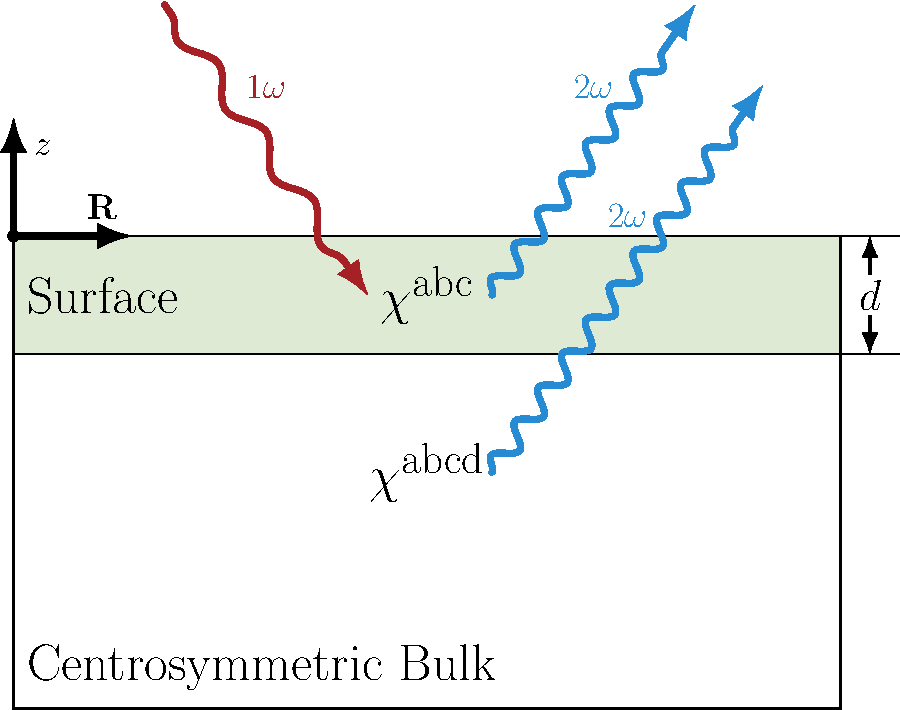
\includegraphics[scale=0.6]{content/figures/diag-system}
\caption{Sketch of a semi-infinite system with a centrosymmetric bulk. The
surface region is of width $\sim l$. The incoming photon of frequency $\omega$
is represented by a downward red arrow, whereas both the surface and bulk
created second-harmonic photons of frequency $2\omega$ are represented by upward
green arrows. The red color suggests an incoming infrared photon with a green
second-harmonic photon. The dipolar ($\chi^{\mathrm{abc}}$), and quadrupolar
($\chi^{\mathrm{abcd}}$) susceptibility tensors are shown in the regions where
they are nonzero. The $z$-axis is perpendicular to the surface and $\mathbf{R}$
is parallel to it.}
\label{fsystem}
\end{figure}


%%%%%%%%%%%%%%%%%%%%%%%%%%%%%%%%%%%%%%%%%%%%%%%%%%%%%%%%%%%%%%%%%%%%%%%%%%%%%%%%
%%%%%%%%%%%%%%%%%%%%%%%%%%%%%%%%%%%%%%%%%%%%%%%%%%%%%%%%%%%%%%%%%%%%%%%%%%%%%%%%

\section{Length Gauge}\label{longi}

We follow the article by Aversa and Sipe \cite{aversaPRB95} to calculate the
optical properties of a given system within the longitudinal gauge. More recent
derivations can also be found in Refs. \cite{sipePRB00} and
\ref{lambrechtPSSB00}. We assume the long-wavelength approximation which implies
a position independent electric field, $\mathbf{E}(t)$. The Hamiltonian in the
length gauge approximation is given by
\begin{equation}\label{ache}
\hat{H}=\hat{H}^{\Sigma}_{0} - e\hat{\mathbf{r}}\cdot\mathbf{E},
\end{equation}
with
\begin{align}\label{ache.1}
  \hat{H}^{\Sigma}_{0} = \hat{H}^{\mathrm{LDA}}_{0}
+ \mathcal{S}(\mathbf{r},\mathbf{p}),
\end{align} 
as the unperturbed Hamiltonian. The LDA Hamiltonian can be expressed as follows,
\begin{align}\label{ache.2}
\hat{H}^{\mathrm{LDA}}_{0}
&= \frac{\hat{p}^{2}}{2m_{e}} + \hat{V}^{\mathrm{ps}},\nonumber\\
\hat{V}^{\mathrm{ps}}
&= \hat{V}^{\mathrm{l}}(\hat{\mathbf{r}}) + \hat{V}^{\mathrm{nl}},
\end{align}  
where $\hat{V}^{\mathrm{l}}(\hat{\mathbf{r}})$ and $\hat{V}^{\mathrm{nl}}$ are
the local and the nonlocal parts of the crystal pseudopotential
$\hat{V}^{\mathrm{ps}}$. For the latter, we have that
\begin{align}\label{ache.3n}
V^{\mathrm{nl}}(\mathbf{r},\mathbf{r}')\equiv
\langle\mathbf{r}\vert
\hat{V}^{\mathrm{nl}}
\vert\mathbf{r}'\rangle \neq 0 
\quad\text{for}\quad\mathbf{r} \neq \mathbf{r}',
\end{align}
where $V^{\mathrm{nl}}(\mathbf{r},\mathbf{r}')$ is a function of $\mathbf{r}$
and $\mathbf{r}'$ representing the nonlocal contribution of the pseudopotential.
The Schr\"odinger equation reads
\begin{align}\label{ache.4} 
\left(
\frac{-\hbar^2}{2m_{e}}\nabla^{2}
+ \hat{V}^l(\mathbf{r})
\right)
\psi_{n\mathbf{k}}(\mathbf{r})
+ \int\hat{V}^{\mathrm{nl}}(\mathbf{r},\mathbf{r}')
  \psi_{n\mathbf{k}}(\mathbf{r}')\,d\mathbf{r}'
= E_{i}\psi_{n\mathbf{k}}(\mathbf{r}),
\end{align} 
where $\psi_{n\mathbf{k}}(\mathbf{r}) = \langle\mathbf{r}|n\mathbf{k}\rangle =
e^{i\mathbf{k}\cdot\mathbf{r}}u_{n\mathbf{k}}(\mathbf{r})$, are the real space
representations of the Bloch states $|n\mathbf{k}\rangle$ labeled by the band
index $n$ and the crystal momentum $\mathbf{k}$, and
$u_{n\mathbf{k}}(\mathbf{r})$ is cell periodic. $m_{e}$ is the bare mass of the
electron. The nonlocal scissors operator is given by
\begin{equation}\label{chon.0}
\mathcal{S}(\mathbf{r},\mathbf{p}) = 
\hbar\Delta\sum_{n}
\int(1 - f_{n}(\mathbf{k}))\vert n\mathbf{k}'\rangle \langle n\mathbf{k}'\vert
\,d^{3}k',
\end{equation}
where $f_{n}(\mathbf{k})$ is the occupation number that is independent of
$\mathbf{k}$ for $T = 0$ K, and is $f_{n} = 1$ for filled bands and $f_{n} = 0$
for unoccupied bands. For semiconductors the filled bands correspond to valence
bands ($n = v$), and unoccupied bands correspond to conduction bands ($n = c$).
We have that
\begin{equation}\label{chon.1}
\begin{split}
H^\mathrm{LDA}_{0}\vert n\mathbf{k}\rangle
    &= \hbar\omega^{\mathrm{LDA}}_{n}(\mathbf{k})\vert n\mathbf{k}\rangle\\
H^{\Sigma}_{0}\vert n\mathbf{k}\rangle
    &= \hbar\omega^{\Sigma}_{n}(\mathbf{k})\vert n\mathbf{k}\rangle,
\end{split}
\end{equation} 
where 
\begin{equation}\label{chon.78}
\hbar\omega^{\Sigma}_{n}(\mathbf{k})
= \hbar\omega^{\mathrm{LDA}}_{n}(\mathbf{k}) + \hbar\Delta(1 - f_{n}),
\end{equation}
is the scissored energy. Here, $\hbar\Delta$ is the value by which the
conduction bands are rigidly ($\mathbf{k}$-independent) shifted upwards in
energy, also known as the scissors shift. $\Delta$ could be taken to be
$\mathbf{k}$ dependent, but for most calculations (like the ones presented
here), a rigid shift is sufficient. We can take $\hbar\Delta = E_{g} -
E_{g}^\mathrm{LDA}$ where $E_{g}$ is the experimental or GW band gap taken at
the $\Gamma$ point, i.e. $\mathbf{k} = 0$. We used the fact that $\vert
n\mathbf{k}\rangle^\mathrm{LDA} \approx \vert n\mathbf{k}\rangle^\Sigma$, thus
negating the need to label the Bloch states with the LDA or $\Sigma$
superscripts. The matrix elements of $\mathbf{r}$ are split between the
\emph{intraband} ($\mathbf{r}_{i}$) and \emph{interband} ($\mathbf{r}_{e}$)
parts, where $\mathbf{r} = \mathbf{r}_{i} + \mathbf{r}_{e}$
\cite{adamsJCP53, blountSSP62, aversaPRB95} and
\begin{align}\label{rnminn}
\langle n\mathbf{k}\vert \hat{\mathbf{r}}_{i} |m\mathbf{k}'\rangle 
&= \delta_{nm}
\left[
  \delta(\mathbf{k} - \mathbf{k}')\boldsymbol{\xi}_{nn}(\mathbf{k})
+ i\nabla_{\mathbf{k}}\delta(\mathbf{k} - \mathbf{k}')
\right],\\
\langle n\mathbf{k}| \hat{\mathbf{r}}_{e} |m\mathbf{k}'\rangle 
&= (1- \delta_{nm})\delta(\mathbf{k}-\mathbf{k}')
   \boldsymbol{\xi}_{nm}(\mathbf{k}),\label{rnmenn}
\end{align}
with
\begin{equation}\label{zetann}
\boldsymbol{\xi}_{nm}(\mathbf{k})
\equiv i\frac{(2\pi)^3}{\Omega}
\int_{\Omega}u^{*}_{n\mathbf{k}}(\mathbf{r})
\nabla_{\mathbf{k}}\,u_{m\mathbf{k}}(\mathbf{r})
\,d\mathbf{r},
\end{equation}
where $\Omega$ is the unit cell volume. The interband part, $\mathbf{r}_{e}$,
can be obtained as follows. We start by introducing the velocity operator
\begin{align}\label{vop}
\hat{\mathbf{v}}^{\Sigma} &=
\frac{1}{i\hbar}\left[\hat{\mathbf{r}},\hat{H}^{\Sigma}_{0}\right],
\end{align}
and calculating its matrix elements
\begin{equation}\label{conhrnm}
i\hbar\langle n\mathbf{k}\vert\mathbf{v}^\Sigma\vert m\mathbf{k}\rangle
= \langle n\mathbf{k}\vert
\left[
\hat{\mathbf{r}}, \hat{H}^{\Sigma}_{0}
\right]
  \vert m\mathbf{k}\rangle
= \langle n\mathbf{k}\vert
\hat{\mathbf{r}}\hat{H}^{\Sigma}_{0} - \hat{H}^{\Sigma}_{0}\hat{\mathbf{r}}
\vert m\mathbf{k}\rangle
=
\left(
\hbar\omega^{\Sigma}_{m}(\mathbf{k}) - \hbar\omega^{\Sigma}_{n}(\mathbf{k})
\right)
\langle n\mathbf{k}\vert\hat{\mathbf{r}}\vert m\mathbf{k}\rangle.
\end{equation}
Defining $\omega^\Sigma_{nm}(\mathbf{k}) =
\omega^{\Sigma}_{n}(\mathbf{k}) - \omega^\Sigma_m(\mathbf{k})$, we get
\begin{equation}\label{pmnrmn}
\mathbf{r}_{nm}(\mathbf{k})
= \frac{\mathbf{v}^\Sigma_{nm}(\mathbf{k})}{i\omega^\Sigma_{nm}(\mathbf{k})}
\qquad n\notin D_{m},
\end{equation} 
which can be identified as
$\mathbf{r}_{nm}=(1-\delta_{nm})\boldsymbol{\xi}_{nm}\to \mathbf{r}_{e,nm}$.
Here, $D_m$ are all the possible degenerate $m$-states. When $\mathbf{r}_{i}$
appears in commutators we use \cite{aversaPRB95}
\begin{equation}\label{conmri3n}
\langle n\mathbf{k}\vert
\left[
\hat{\mathbf{r}}_{i}, \hat{\mathcal{O}}
\right]
\vert m\mathbf{k}'\rangle
= i\delta(\mathbf{k} - \mathbf{k}')(\mathcal{O}_{nm})_{;\mathbf{k}},
\end{equation}  
with
\begin{equation}\label{gendevnn}
(\mathcal{O}_{nm})_{;\mathbf{k}} =
  \nabla_{\mathbf{k}}\mathcal{O}_{nm}(\mathbf{k})
- i\mathcal{O}_{nm}(\mathbf{k})
\left(
\boldsymbol{\xi}_{nn}(\mathbf{k}) - \boldsymbol{\xi}_{mm}(\mathbf{k})
\right),
\end{equation} 
where ``$;\mathbf{k}$'' denotes the generalized derivative (see Appendix
\ref{app:re_ri}).

As can be seen from Eq. \eqref{ache.1} and \eqref{ache.2}, both $\mathcal{S}$
and $\hat{V}^{\mathrm{nl}}$ are nonlocal potentials. Their contribution in the
calculation of the optical response has to be considered in order to get
reliable results \cite{ismailPRL01}. We proceed as follows: from Eqs.
\eqref{vop}, \eqref{ache.1} and \eqref{ache.2} we find
\begin{align}\label{vop2}
\hat{\mathbf{v}}^{\Sigma} &=
\frac{\hat{\mathbf{p}}}{m_{e}} + \frac{1}{i\hbar}
\left[\hat{\mathbf{r}},\hat{V}^{\mathrm{nl}}(\mathbf{r},\mathbf{r}')\right]
+ \frac{1}{i\hbar}
  \left[\hat{\mathbf{r}},\hat{\mathcal{S}}(\mathbf{r},\mathbf{p})\right]
\nonumber\\
&\equiv
\hat{\mathbf{v}} + \hat{\mathbf{v}}^{\mathrm{nl}} + \hat{\mathbf{v}}^\mathcal{S}
= \hat{\mathbf{v}}^\mathrm{LDA} + \hat{\mathbf{v}}^\mathcal{S},
\end{align}
where we have defined
\begin{equation}\label{conhr}
\begin{split}
\hat{\mathbf{v}} &=\frac{\hat{\mathbf{p}}}{m_{e}}\\
\hat{\mathbf{v}}^{\mathrm{nl}} &= \frac{1}{i\hbar}
  \left[\hat{\mathbf{r}},\hat{V}^{\mathrm{nl}}\right]\\
\hat{\mathbf{v}}^\mathcal{S} &= \frac{1}{i\hbar}
  \left[\hat{\mathbf{r}},\hat{S}(\mathbf{r},\mathbf{p})\right]\\
\hat{\mathbf{v}}^\mathrm{LDA} &= \hat{\mathbf{v}}+\hat{\mathbf{v}}^{\mathrm{nl}}
\end{split}
\end{equation}  
with $\hat{\mathbf{p}}= -i\hbar\boldsymbol{\nabla}$ the momentum operator. Using
Eq. \eqref{chon.0}, we obtain that the matrix elements of
$\hat{\mathbf{v}}^\mathcal{S}$ are given by
\begin{equation}\label{chon.2} 
\mathbf{v}^\mathcal{S}_{nm} = i\Delta f_{mn}\mathbf{r}_{nm},
\end{equation}
with $f_{nm} = f_{n} - f_{m}$, where we see that $\mathbf{v}^\mathcal{S}_{nn} =
0$, then
\begin{align}\label{chon.8}
\mathbf{v}^\Sigma_{nm} 
&= \mathbf{v}^\mathrm{LDA}_{nm} + i\Delta f_{mn}\mathbf{r}_{nm}\nonumber\\
&= \mathbf{v}^\mathrm{LDA}_{nm} + i\Delta f_{mn}
   \frac{\mathbf{v}^\Sigma_{nm}(\mathbf{k})}{i\omega^\Sigma_{nm}(\mathbf{k})}
   \nonumber\\
%%%%%%%%%%%%%%%%%%%%%%%%%%%%%%%%%%%%%%%%%%%%%%%%%
\mathbf{v}^\Sigma_{nm}
  \frac{\omega^\Sigma_{nm}-\Delta f_{mn}}{\omega^\Sigma_{nm}}
&= \mathbf{v}^\mathrm{LDA}_{nm}\nonumber\\
%%%%%%%%%%%%%%%%%%%%%%%%%%%%%%%%%%%%%%%%%%%%%%%%%
\mathbf{v}^\Sigma_{nm}\frac{\omega^{\mathrm{LDA}}_{nm}}{\omega^\Sigma_{nm}}
&= \mathbf{v}^\mathrm{LDA}_{nm}\nonumber\\
%%%%%%%%%%%%%%%%%%%%%%%%%%%%%%%%%%%%%%%%%%%%%%%%%
\frac{\mathbf{v}^\Sigma_{nm}}{\omega^\Sigma_{nm}}
&= \frac{\mathbf{v}^\mathrm{LDA}_{nm}}{\omega^{\mathrm{LDA}}_{nm}},
\end{align}
since $\omega^\Sigma_{nm}-\Delta f_{mn}=\omega^{\mathrm{LDA}}_{nm}$. Therefore,
\begin{align}\label{chon.9}
\begin{split}
\mathbf{v}^\Sigma_{nm}(\mathbf{k}) &=
\frac{\omega^\Sigma_{nm}}{\omega^{\mathrm{LDA}}_{nm}}
\mathbf{v}^\mathrm{LDA}_{nm}(\mathbf{k})
= \left(
1 + \frac{\Delta}{\omega_c(\mathbf{k})-\omega_v(\mathbf{k})}
\right)
\mathbf{v}^\mathrm{LDA}_{nm}(\mathbf{k})\qquad n\notin D_{m}\\\\
\mathbf{v}^\Sigma_{nn}(\mathbf{k}) &= \mathbf{v}^\mathrm{LDA}_{nn}(\mathbf{k}),
\end{split}
\end{align} 
and Eq. \eqref{pmnrmn} gives
\begin{align}\label{chon.10}
\mathbf{r}_{nm}(\mathbf{k})
= \frac{\mathbf{v}^\Sigma_{nm}(\mathbf{k})}{i\omega^\Sigma_{nm}(\mathbf{k})}
= \frac{\mathbf{v}^\mathrm{LDA}_{nm}(\mathbf{k})}
{i\omega^{\mathrm{LDA}}_{nm}(\mathbf{k})} \qquad n\notin D_{m}.
\end{align}
The matrix elements of $\mathbf{r}_{e}$ are the same whether we use the LDA or
the scissored Hamiltonian. Therefore, there is no need to label them with either
LDA or $S$ superscripts. Thus, we can write
\begin{equation}\label{chon.98}
\mathbf{r}_{e,nm}\to\mathbf{r}_{nm}(\mathbf{k}) =
\frac{\mathbf{v}^\mathrm{LDA}_{nm}(\mathbf{k})}
     {i\omega^{\mathrm{LDA}}_{nm}(\mathbf{k})}
\qquad n\notin D_{m},
\end{equation}   
which gives the interband matrix elements of the position operator in terms of
the matrix elements of $\hat{\mathbf{v}}^\mathrm{LDA}$. These matrix elements
include the matrix elements of $\mathbf{v}^{\mathrm{nl}}_{nm}(\mathbf{k})$ which
can be readily calculated for fully separable nonlocal pseudopotentials in the
Kleinman-Bylander form \cite{mottaCMS10, kleinmanPRL82, adolphPRB96}. In
Appendix \ref{appvnl} we outline how this is accomplished.


%%%%%%%%%%%%%%%%%%%%%%%%%%%%%%%%%%%%%%%%%%%%%%%%%%%%%%%%%%%%%%%%%%%%%%%%%%%%%%%%
%%%%%%%%%%%%%%%%%%%%%%%%%%%%%%%%%%%%%%%%%%%%%%%%%%%%%%%%%%%%%%%%%%%%%%%%%%%%%%%%

% @@@@@@@@@@@@@@@@@@@@@@@@@@@@@@@@@@@@@@@@@@@@@@@@@@@@@@@@@@@@@@@@@@@@@@@@@@@@@@
% @@@@@@@@@@@@@@@@@@@@@@@@@@@@@@@@@@@@@@@@@@@@@@@@@@@@@@@@@@@@@@@@@@@@@@@@@@@@@@
% @@@@@@@@@@@@@@@@@@@@@@@@@@@@@@@@@@@@@@@@@@@@@@@@@@@@@@@@@@@@@@@@@@@@@@@@@@@@@@
% @@@@@@@@@@@@@@@@@@@@@@@@@@@@@@@@@@@@@@@@@@@@@@@@@@@@@@@@@@@@@@@@@@@@@@@@@@@@@@
% @@@@@@@@@@@@@@@@@@@@@@@@@@@@@@@@@@@@@@@@@@@@@@@@@@@@@@@@@@@@@@@@@@@@@@@@@@@@@@
% @@@@@@@@@@@@@@@@@@@@@@@@@@@@@@@@@@@@@@@@@@@@@@@@@@@@@@@@@@@@@@@@@@@@@@@@@@@@@@

\section{Time-dependent Perturbation Theory}\label{tdpt}

In the independent particle approximation, we use the electron density
operator $\hat{\rho}$ to obtain the expectation value of any observable
$\mathcal{O}$ as
\begin{equation}\label{traza}
\mathcal{O}=\mathrm{Tr}(\hat{\mathcal{O}}\hat{\rho})=\mathrm{Tr}(\hat{\rho}\hat{\mathcal{O}}),
\end{equation}
where $\mathrm{Tr}$ is the trace and is invariant under cyclic permutations.
The dynamic equation of motion for $\rho$ is given by
\begin{equation}\label{eqrho}
i\hbar \frac{d\hat{\rho}}{dt}=[\hat{H},\hat{\rho}]
,
\end{equation}
where it is more convenient to work in the interaction picture. We transform 
all operators according to 
\begin{equation}\label{ip}
\hat{\mathcal{O}}_I=\hat{U}\hat{\mathcal{O}}\hat{U}^\dagger,
\end{equation}
where
\begin{equation}\label{ou}
\hat{U}=e^{i\hat{H}_0t/\hbar},
\end{equation}
is the unitary operator that shifts us to the interaction picture.
Note that $\hat{\mathcal{O}}_I$ depends on time even if $\hat{\mathcal{O}}$ does not.
Then, we transform Eq. \eqref{eqrho} into
\begin{equation}\label{intrho}
i\hbar\frac{d\hat{\rho}_I(t)}{dt}=[-e\hat{\mathbf{r}}_I(t)\cdot\mathbf{E}(t),\hat{\rho}_I(t)],
\end{equation}
that leads to
\begin{equation}\label{intrho2}
\hat{\rho}_I(t)=\hat{\rho}_I(t=-\infty)
+
\frac{ie}{\hbar}\int_{-\infty}^t dt'[\hat{\mathbf{r}}_I(t')\cdot\mathbf{E}(t'),\hat{\rho}_I(t')].
\end{equation}
We assume that the interaction is switched-on adiabatically and
choose a time-periodic perturbing field, to write
\begin{equation}\label{efield}
\mathbf{E}(t)=\mathbf{E} e^{-i\omega t}e^{\eta t}=\mathbf{E} e^{-i\tilde{\omega} t}
,
\end{equation}
with
\begin{equation}\label{got}
\tilde{\omega}=\omega+i\eta
,
\end{equation} 
where $\eta > 0$ assures
that at $t=-\infty$ the interaction is zero and has its full strength $\mathbf{E}$ 
at $t=0$. After computing the required time integrals one takes
$\eta\to 0$. 
Also, $\hat{\rho}_I(t=-\infty)$ should be time independent and thus 
$[\hat{H},\hat{\rho}]_{t=-\infty}=0$, This implies that 
$\hat{\rho}_I(t=-\infty)=\hat{\rho}(t=-\infty)\equiv\hat{\rho}_0$,
where $\hat{\rho}_0$ is
the density matrix of the unperturbed ground state,
such that
\begin{equation}\label{nrhon}
\langle n\mathbf{k}| \hat{\rho}_{0} |m\mathbf{k}'\rangle = f_{n}(\hbar\omega^{\Sigma}_{n}(\mathbf{k}))\delta_{nm}\delta(\mathbf{k}-\mathbf{k}')
,
\end{equation}
with $f_{n}(\hbar\omega^{\Sigma}_{n}(\mathbf{k}))=f_{n\mathbf{k}}$ as the Fermi-Dirac distribution function.

We solve Eq. \eqref{intrho2} using the standard iterative
solution, for which we write
\begin{equation}\label{rhop}
\hat{\rho}_{I} = \hat{\rho}_{I}^{(0)} + \hat{\rho}_{I}^{(1)} + \hat{\rho}_{I}^{(2)} + \cdots
,
\end{equation}
where $\hat{\rho}_{I}^{(N)}$ is the density operator to order $N$ in $\mathbf{E}(t)$.
Then, Eq. \eqref{intrho2} reads
\begin{equation}\label{intrho3}
\hat{\rho}_{I}^{(0)} + \hat{\rho}_{I}^{(1)} + \hat{\rho}_{I}^{(2)} + \cdots
= \hat{\rho}_{0}
+
\frac{ie}{\hbar}\int_{-\infty}^t dt'[\hat{\mathbf{r}}_I(t')\cdot\mathbf{E}(t'),
\hat{\rho}_I^{(0)}+\hat{\rho}_I^{(1)}+\hat{\rho}_I^{(2)}+\cdots
]
,
\end{equation}
where, by equating equal orders in the perturbation, we find
\begin{equation}\label{rho0}
\hat{\rho}_I^{(0)}\equiv\hat{\rho}_0
,
\end{equation}
and
\begin{equation}\label{rhoN}
\hat{\rho}_I^{(N)}(t)=
\frac{ie}{\hbar}
\int_{-\infty}^t dt'[\hat{\mathbf{r}}_I(t')\cdot\mathbf{E}(t'),\hat{\rho}^{(N-1)}_I(t')].
\end{equation}
It is simple to show that matrix elements of Eq. (\ref{rhoN}) satisfy
$\langle n\mathbf{k}| \rho_I^{(N+1)}(t) |m\mathbf{k}'\rangle = \rho^{(N+1)}_{I,nm}(\mathbf{k})\delta(\mathbf{k}-\mathbf{k}')$,
with
\begin{equation}\label{rtilde}
\rho^{(N+1)}_{I,nm}(\mathbf{k};t)
=\frac{ie}{\hbar}\int_{-\infty}^t dt'
\langle n\mathbf{k}|
[\hat{\mathbf{r}}_I(t'),\hat{\rho}^{(N)}_I(t')]
|m\mathbf{k}\rangle
\cdot\mathbf{E}(t')
.
\end{equation}

We now work out the commutator of Eq. \eqref{rtilde}. Then,
\begin{align}\label{conmu1}
\langle n\mathbf{k}|
[\hat{\mathbf{r}}_I(t),\hat{\rho}^{(N)}_I(t)]
|m\mathbf{k}\rangle
&=
\langle n\mathbf{k}|
[\hat{U}\hat{\mathbf{r}}\hat{U}^\dagger,\hat{U}\hat{\rho}^{(N)}(t)\hat{U}^\dagger]
|m\mathbf{k}\rangle
\nonumber \\
&=
\langle n\mathbf{k}|
\hat{U}[\hat{\mathbf{r}},\hat{\rho}^{(N)}(t)]\hat{U}^\dagger
|m\mathbf{k}\rangle
\\
&=
e^{i\omega^\Sigma_{nm\mathbf{k}}t}
\left(
\langle n\mathbf{k}|
[\hat{\mathbf{r}}_e,\hat{\rho}^{(N)}(t)]
+
[\hat{\mathbf{r}}_i,\hat{\rho}^{(N)}(t)]
|m\mathbf{k}\rangle
\right)
\nonumber
.
\end{align}
% where the time dependence of operator's interaction picture is
% explicitly shown by the exponential factor, and the implicit
% dependence of $\hat{\rho}^{(N)}$ inherited from Eq. \eqref{eqrho} is
% shown by its $t$ argument.
We calculate the interband term first, so using Eq. \eqref{chon.98} we obtain
\begin{align}\label{conmu2}
\langle n\mathbf{k}|
[\hat{\mathbf{r}}_e,\hat{\rho}^{(N)}(t)]
|m\mathbf{k}\rangle
&=
\sum_{\ell}
\left(
\langle n\mathbf{k}|
\hat{\mathbf{r}}_e
|\ell\mathbf{k}\rangle
\langle \ell\mathbf{k}|
\hat{\rho}^{(N)}(t)
|m\mathbf{k}\rangle
\right.
\nonumber \\
&
\left.
-
\langle n\mathbf{k}|
\hat{\rho}^{(N)}(t)
|\ell\mathbf{k}\rangle
\langle \ell\mathbf{k}|
\hat{\mathbf{r}}_e
|m\mathbf{k}\rangle
\right)
\nonumber \\
&=
\sum_{\ell\ne n,m}
\left(
\mathbf{r}_{n\ell}(\mathbf{k})
\rho^{(N)}_{\ell m}(\mathbf{k};t)
-
\rho^{(N)}_{n\ell}(\mathbf{k};t)
\mathbf{r}_{\ell m}(\mathbf{k})
\right)
\nonumber\\
&\equiv
\mathbf{R}^{(N)}_e(\mathbf{k};t)
,
\end{align}

and from Eq. \eqref{conmri3n},
\begin{equation}\label{conmri4}
\langle n\mathbf{k}|
[\hat{\mathbf{r}}_i,\hat{\rho}^{(N)}(t)]
|m\mathbf{k}'\rangle
=i \delta(\mathbf{k}-\mathbf{k}') (\rho^{(N)}_{nm}(t))_{;\mathbf{k}}
\equiv \delta(\mathbf{k}-\mathbf{k}')\mathbf{R}_i^{(N)}(\mathbf{k};t)
.
\end{equation}
Then Eq. \eqref{rtilde} becomes
\begin{equation}\label{rtilde2}
\rho^{(N+1)}_{I,nm}(\mathbf{k};t)
=\frac{ie}{\hbar}\int_{-\infty}^t dt'
e^{i(\omega^\Sigma_{nm\mathbf{k}}-\tilde{\omega})t'}
\left[R_e^{\mathrm{b}(N)}(\mathbf{k};t')+R_i^{\mathrm{b}(N)}(\mathbf{k};t')\right]E^{\mathrm{b}}
,
\end{equation}
where the roman superindices
$\mathrm{a},\mathrm{b},\mathrm{c}$ denote Cartesian components that are summed over if repeated.
Starting from the linear response and proceeding from Eq. \eqref{nrhon} and  \eqref{conmu2},
\begin{align}\label{R0e}
R_e^{\mathrm{b}(0)}(\mathbf{k};t)
&=
\sum_{\ell}
\left(
r^{\mathrm{b}}_{n\ell}(\mathbf{k})
\rho^{(0)}_{\ell m}(\mathbf{k})
-
\rho^{(0)}_{n\ell}(\mathbf{k})
r^{\mathrm{b}}_{\ell m}(\mathbf{k})
\right)
\nonumber \\
&=
\sum_{\ell}
\left(
r^{\mathrm{b}}_{n\ell}(\mathbf{k})
\delta_{\ell m}f_m(\hbar\omega^\Sigma_m(\mathbf{k}))
-
\delta_{n\ell}f_n(\hbar\omega^{\Sigma}_{n}(\mathbf{k}))
r^{\mathrm{b}}_{\ell m}(\mathbf{k})
\right)
\nonumber \\
&=
f_{mn\mathbf{k}}
r^{\mathrm{b}}_{nm}(\mathbf{k})
,
\end{align}
where $f_{mn\mathbf{k}}=f_{m\mathbf{k}}-f_{n\mathbf{k}}$.
From now on,
it should be clear that the matrix elements of $\mathbf{r}_{nm}$ imply
$n\notin D_m$.
We also have from Eq. \eqref{conmri4} and Eq. \eqref{gendevnn} that
\begin{equation}\label{R0i}
R_i^{\mathrm{b}(0)}(\mathbf{k})=i(\rho^{(0)}_{nm})_{;k^{\mathrm{b}}}=i\delta_{nm}(f_{n\mathbf{k}})_{;k^{\mathrm{b}}}=i\delta_{nm}\nabla_{k^{\mathrm{b}}} f_{n\mathbf{k}}
.
\end{equation}
For a semiconductor at $T=0$, $f_{n\mathbf{k}}$ is one if the state
$|n\mathbf{k}\rangle$ is a valence state and zero if it is a conduction state; 
thus $\nabla_\mathbf{k} f_{n\mathbf{k}}=0$ and $\mathbf{R}_i^{(0)}=0$ and
the linear response has no contribution from
intraband transitions.
 Then,
\begin{align}\label{rtilde2n}
\rho^{(1)}_{I,nm}(\mathbf{k};t)
&=\frac{ie}{\hbar}
f_{mn\mathbf{k}}
r^{\mathrm{b}}_{nm}(\mathbf{k})E^{\mathrm{b}}
\int_{-\infty}^t dt'
e^{i(\omega^\Sigma_{nm\mathbf{k}}-\tilde{\omega})t'}
\nonumber \\
&=\frac{e}{\hbar}
f_{mn\mathbf{k}}
r^{\mathrm{b}}_{nm}(\mathbf{k})E^{\mathrm{b}}
\frac{e^{i(\omega^\Sigma_{nm\mathbf{k}}-\tilde{\omega})t}}
{\omega^\Sigma_{nm\mathbf{k}}-\tilde{\omega}}
\nonumber \\
&=
e^{i\omega^\Sigma_{nm\mathbf{k}}t}
B^{\mathrm{b}}_{mn}(\mathbf{k})E^{\mathrm{b}}(t)
\nonumber \\
&=
e^{i\omega^\Sigma_{nm\mathbf{k}}t}
\rho^{(1)}_{nm}(\mathbf{k};t)
,
\end{align}
with
\begin{equation}\label{rho1} 
B^{\mathrm{b}}_{nm}(\mathbf{k},\omega)=
\frac{e}{\hbar}\frac{f_{mn\mathbf{k}}r^{\mathrm{b}}_{nm}(\mathbf{k})}{\omega^\Sigma_{nm\mathbf{k}}-\tilde{\omega}}
,
\end{equation} 
and
\begin{equation}\label{rhonoi1}
\rho^{(1)}_{nm}(\mathbf{k};t)=B^{\mathrm{b}}_{mn}(\mathbf{k},\omega)E^{\mathrm{b}}(\omega)e^{-i\tilde{\omega} t}
.
\end{equation}

Now, we calculate the second-order response. Then, from Eq. \eqref{conmu2}
\begin{align}\label{R1e}
R_e^{\mathrm{b}(1)}(\mathbf{k};t)
&=
\sum_{\ell}
\left(
r^{\mathrm{b}}_{n\ell}(\mathbf{k})
\rho^{(1)}_{\ell m}(\mathbf{k};t)
-
\rho^{(1)}_{n\ell}(\mathbf{k};t)
r^{\mathrm{b}}_{\ell m}(\mathbf{k})
\right)
\nonumber \\
&=
\sum_{\ell}
\left(
r^{\mathrm{b}}_{n\ell}(\mathbf{k})
B^{\mathrm{c}}_{\ell m}(\mathbf{k},\omega)
-
B^{\mathrm{c}}_{n\ell}(\mathbf{k},\omega)
r^{\mathrm{b}}_{\ell m}(\mathbf{k})
\right)E^{\mathrm{c}}(t)
,
\end{align}
and from Eq. \eqref{conmri4}
\begin{equation}\label{R1i}
R_i^{\mathrm{b}(1)}(\mathbf{k};t)=
i(\rho^{(1)}_{nm}(t))_{;k^{\mathrm{b}}}=
iE^{\mathrm{c}}(t)(B^{\mathrm{c}}_{nm}(\mathbf{k},\omega))_{;k^{\mathrm{b}}}
.
\end{equation}

Using Eqs. \eqref{R1e} and  \eqref{R1i} in Eq. (\ref{rtilde2}),
we obtain
\begin{align}\label{rtilde33}
\rho^{(2)}_{I,nm}(\mathbf{k};t)
&=
\frac{ie}{\hbar}
\bigg[
\sum_{\ell}
\Big(
r^{\mathrm{b}}_{n\ell}(\mathbf{k})
B^{\mathrm{c}}_{\ell m}(\mathbf{k},\omega)
-
B^{\mathrm{c}}_{n\ell}(\mathbf{k},\omega)
r^{\mathrm{b}}_{\ell m}(\mathbf{k})
\Big)
\nonumber \\
&+
i
(B^{\mathrm{c}}_{nm}(\mathbf{k},\omega))_{;k^{\mathrm{b}}}
\bigg]
E^{\mathrm{b}}_{\omega}E_{\omega}^{\mathrm{c}}
\int_{-\infty}^t dt'
e^{i(\omega^\Sigma_{nm\mathbf{k}}-2\tilde{\omega})t'}
\nonumber \\
&=
\frac{e}{\hbar}
\bigg[
\sum_{\ell}
\Big(
r^{\mathrm{b}}_{n\ell}(\mathbf{k})
B^{\mathrm{c}}_{\ell m}(\mathbf{k},\omega)
-
B^{\mathrm{c}}_{n\ell}(\mathbf{k},\omega)
r^{\mathrm{b}}_{\ell m}(\mathbf{k})
\Big)
\nonumber \\
&+
i
(B^{\mathrm{c}}_{nm}(\mathbf{k},\omega))_{;k^{\mathrm{b}}}
\bigg]
E^{\mathrm{b}}_{\omega}E_{\omega}^{\mathrm{c}}
\frac{e^{i(\omega^\Sigma_{nm\mathbf{k}}-2\tilde{\omega})t}}
{\omega^\Sigma_{nm\mathbf{k}}-2\tilde{\omega}}
\nonumber \\
&=
e^{i\omega^\Sigma_{nm\mathbf{k}}t}
\rho_{nm}^{(2)}(\mathbf{k};t)
.
\end{align}
Now, we write
$\rho_{nm}^{(2)}(\mathbf{k};t)=\rho_{nm}^{(2)}(\mathbf{k};2\omega)e^{-i2\tilde{\omega} t}$,
with
\begin{align}\label{rho2}
\rho_{nm}^{(2)}(\mathbf{k};2\omega)&=\frac{e}{i\hbar}\frac{1}{\omega^\Sigma_{nm\mathbf{k}}-2\tilde{\omega}}
\bigg[-(B_{nm}^{\mathrm{c}}(\mathbf{k},\omega)_{;k^{\mathrm{b}}}
\nonumber \\
&
+i\sum_\ell\Big(r_{n\ell}^{\mathrm{b}}B_{\ell m}^{\mathrm{c}}(\mathbf{k},\omega) - B_{n\ell}^{\mathrm{c}}(\mathbf{k},\omega)
  r_{\ell m}^{\mathrm{b}}\Big)
\bigg] 
E^{\mathrm{b}}(\omega)E^{\mathrm{c}}(\omega)
\end{align} 
where 
$B_{\ell m}^{\mathrm{a}}(\mathbf{k},\omega)$ are given by Eq. \eqref{rho1}. 
We remark that $\mathbf{r}_{nm}(\mathbf{k})$  are
the same whether calculated with the LDA or the scissored Hamiltonian. 
We chose the former in this article.

\section{Layered Current Density}\label{cd}

In this section, we derive the expressions for the microscopic current density
of a given layer in the unit cell of the system. The approach we use to study
the surface of a semi-infinite semiconductor crystal is as follows. Instead of
using a semi-infinite system, we replace it by a slab (see Fig. \ref{fslab}).
The slab consists of a front and back surface, and in between these two surfaces
is the bulk of the system. In general the surface of a crystal reconstructs or
relaxes as the atoms move to find equilibrium positions. This is due to the fact
that the otherwise balanced forces are disrupted when the surface atoms do not
find their partner atoms that are now absent at the surface of the slab.

To take the reconstruction or relaxation into account, we take ``surface'' to
mean the true surface of the first layer of atoms, and some of the atomic
sub-layers adjacent to it. Since the front and the back surfaces of the slab are
usually identical the total slab is centrosymmetric. This implies that
$\chi^{\mathrm{slab}}_{\mathrm{abc}}=0$, and thus we must find a way to bypass
this characteristic of a centrosymmetric slab in order to have a finite
$\chi^s_{\mathrm{abc}}$ representative of the surface. Even if the front and
back surfaces of the slab are different, breaking the centrosymmetry and
therefore giving an overall $\chi^{\mathrm{slab}}_{\mathrm{abc}}\ne 0$, we still
need a procedure to extract the front surface $\chi^f_{\mathrm{abc}}$ and the
back surface $\chi^b_{\mathrm{abc}}$ from the nonlinear susceptibility $\chi^{\mathrm{slab}}_{\mathrm{abc}}=\chi^f_{\mathrm{abc}}-\chi^b_{\mathrm{abc}}$ of the
entire slab.

A convenient way to accomplish the separation of the SH signal of either surface
is to introduce a ``cut function'', $\mathcal{C}(z)$, which is usually taken to be
unity over one half of the slab and zero over the other half.\cite{reiningPRB94}
In this case $\mathcal{C}(z)$ will give the contribution of the side of the slab for
which $\mathcal{C}(z)=1$. We can generalize this simple choice for $\mathcal{C}(z)$ by a
top-hat cut function $\mathcal{C}^{\ell}(z)$ that selects a given layer,
\begin{equation}
\label{sz}
\mathcal{C}^{\ell}(z)=\Theta(z-z_\ell+\Delta_\ell^{\mathrm{b}})
            \Theta(z_\ell-z+\Delta_\ell^f),
\end{equation}
where $\Theta$ is the Heaviside function. Here, $\Delta_\ell^{f/b}$
is the distance that the $\ell$-th layer extends towards the front
$(f)$ or back $(b)$ from its $z_\ell$ position. 
$\Delta_\ell^f+\Delta_\ell^b$ is the thickness of layer $\ell$ 
(see Fig. \ref{fslab}).
\begin{figure}[b]
\centering
%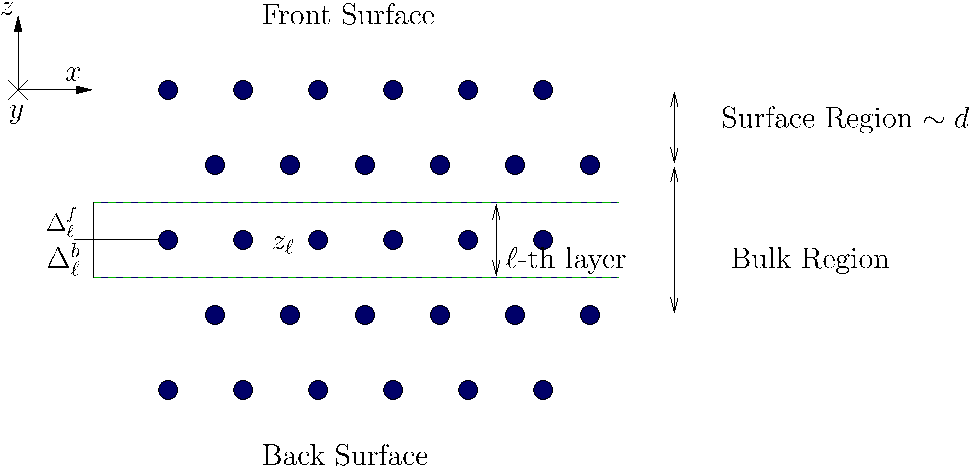
\includegraphics[height=5cm,width=7cm]{slab}
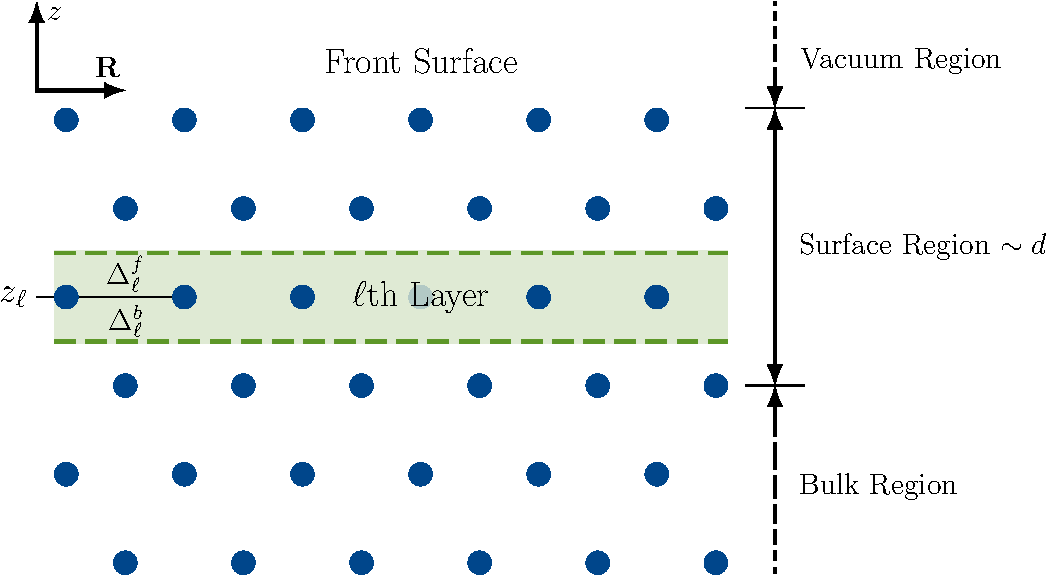
\includegraphics[scale=.7]{content/figures/diag-slab}
\caption{A sketch of a slab where the circles represent atoms.\label{fslab}}
\end{figure}

Now, we show how this ``cut function'' $\mathcal{C}^{\ell}(z)$ is introduced in
the calculation of $\chi_{\mathrm{abc}}$. 
The microscopic current density is given by
\begin{equation}\label{jmic}
\mathbf{j}(\mathbf{r},t)=\mathrm{Tr}(\hat{\mathbf{j}}(\mathbf{r})\hat{\rho}(t)),
\end{equation}
where the operator for the electron's current is
\begin{equation}\label{hatjmic}
\hat{\mathbf{j}}(\mathbf{r})=\frac{e}{2}\left(\hat{\mathbf{v}}^{\Sigma} |\mathbf{r}\rangle\langle\mathbf{r}|
+ |\mathbf{r}\rangle\langle\mathbf{r}|\hat{\mathbf{v}}^{\Sigma}\right), 
\end{equation}
where $\hat{\mathbf{v}}^{\Sigma}$ is the electron's velocity operator to be dealt
with below. We define
$\hat{\mu} \equiv |\mathbf{r}\rangle\langle\mathbf{r}|$ and use the cyclic invariance of
the trace to write
\begin{align}\label{jmic2}
\mathrm{Tr}(\hat{\mathbf{j}}(\mathbf{r})\hat{\rho}(t)
&= \mathrm{Tr}(\hat{\rho}(t)\hat{\mathbf{j}}(\mathbf{r}))
= \frac{e}{2}
\left(
  \mathrm{Tr}(\hat{\rho}\hat{\mathbf{v}}^{\Sigma}\hat{\mu})
+ \mathrm{Tr}(\hat{\rho}\hat{\mu}\hat{\mathbf{v}}^{\Sigma})
\right)\nonumber\\
&= \frac{e}{2}\sum_{n\mathbf{k}}
\left(
\langle n\mathbf{k}| \hat{\rho}\hat{\mathbf{v}}^{\Sigma}\hat{\mu} |n\mathbf{k}\rangle
+ \langle n\mathbf{k}| \hat{\rho}\hat{\mu}\hat{\mathbf{v}}^{\Sigma} |n\mathbf{k}\rangle
\right)\nonumber\\
&= \frac{e}{2}\sum_{nm\mathbf{k}}\langle n\mathbf{k}|\hat{\rho} |m\mathbf{k}\rangle
\left(
\langle m\mathbf{k}| \hat{\mathbf{v}}^{\Sigma}|\mathbf{r}\rangle \langle\mathbf{r}|n\mathbf{k}\rangle
+ \langle m\mathbf{k}|\mathbf{r}\rangle \langle\mathbf{r}| \hat{\mathbf{v}}^{\Sigma} |n\mathbf{k}\rangle
\right)
\nonumber\\
\mathbf{j}(\mathbf{r},t)
&= \sum_{nm\mathbf{k}}\rho_{nm}(\mathbf{k};t)\mathbf{j}_{mn}(\mathbf{k};\mathbf{r}),
\end{align}
where
\begin{equation}\label{jmic3}
\mathbf{j}_{mn}(\mathbf{k};\mathbf{r})=
\frac{e}{2}
\left(
\langle m\mathbf{k}| \hat{\mathbf{v}}^{\Sigma} |\mathbf{r}\rangle \langle\mathbf{r}|n\mathbf{k}\rangle
+
\langle m\mathbf{k}|\mathbf{r}\rangle \langle\mathbf{r}| \hat{\mathbf{v}}^{\Sigma} |n\mathbf{k}\rangle
\right),
\end{equation}
are the matrix elements of the microscopic current operator,
and we have used the fact that the matrix elements between states $|n\mathbf{k}\rangle$
are diagonal in $\mathbf{k}$, i.e. proportional to $\delta(\mathbf{k}-\mathbf{k}')$.

Integrating the microscopic current $\mathbf{j}(\mathbf{r},t)$ over
the entire slab gives the averaged microscopic current density. 
If we want the contribution from only one region of the unit cell 
towards the total current, we can integrate $\mathbf{j}({\mathbf r},t)$ 
over the desired region. The contribution to the current density from the
$\ell$-th layer of the slab is given by
\begin{equation}\label{jsz}
\frac{1}{\Omega}\int d^3r\, \mathcal{C}^{\ell}(z)\, \mathbf{j}(\mathbf{r},t)
 \equiv \mathbf{J}^{\ell}(t),
\end{equation}
where $\mathbf{J}^{\ell}(t)$ is the microscopic current in the
$\ell$-th layer.
Therefore we define
\begin{equation}\label{vcal}
e{\boldsymbol{\mathcal{V}}}^{\Sigma,\ell}_{mn}(\mathbf{k})
\equiv
%\frac{1}{\Omega}
\int d^3r\, \mathcal{C}^{\ell}(z)\,\mathbf{j}_{mn}({\mathbf{k}};\mathbf{r}),
\end{equation}
to write
\begin{equation}\label{jmac}
J_a^{(N,\ell)}(t)=\frac{e}{\Omega}
\sum_{mn\mathbf{k}}
\mathcal{V}^{\Sigma,a,\ell}_{mn}(\mathbf{k})
\rho^{(N)}_{nm}(\mathbf{k};t),
\end{equation}
as the induced microscopic current of the $\ell$-th layer, to order $N$ 
in the external perturbation. The matrix elements of the 
density operator for $N=1,2$ are given by Eqs. \eqref{rho1} and
\eqref{rho2} respectively. 
The Fourier component of microscopic current of Eq. \eqref{jmac} is given by
\begin{equation}\label{jmac2}
J_{\mathrm{a}}^{(N,\ell)}(\omega_3)=\frac{e}{\Omega}
\sum_{mn\mathbf{k}}
\mathcal{V}^{\Sigma,\mathrm{a},\ell}_{mn}(\mathbf{k})
\rho^{(N)}_{nm}(\mathbf{k};\omega_3)
.
\end{equation}
We proceed to give an explicit expression of
$\boldsymbol{\mathcal{V}}^{\Sigma,\ell}_{mn}(\mathbf{k})$.
From
Eqs. \eqref{vcal} and \eqref{jmic3} we obtain
\begin{equation}\label{intj}
{\boldsymbol{\mathcal{V}}}^{\Sigma,\ell}_{mn}({\mathbf k})=
\frac{1}{2}
\int \mathrm{d}^3 r\,
 \mathcal{C}^{\ell}(z)
\bigg[
\langle m\mathbf{k}|\mathbf{v}^\Sigma | \mathbf{r}\rangle
\langle \mathbf{r} | n \mathbf k \rangle +
\langle m\mathbf{k} | \mathbf{r}\rangle
\langle \mathbf{r} | \mathbf{v}^\Sigma | n \mathbf k \rangle\bigg]
,
\end{equation}  
and using the following property
\begin{equation}\label{nl.2}
\langle \mathbf{r} | \hat{\mathbf{v}}^{\Sigma}(\mathbf{r},\mathbf{r}')| n\mathbf{k} \rangle
=\int d^3 r'' \langle\mathbf{r}|\hat{\mathbf{v}}^{\Sigma}(\mathbf{r},\mathbf{r}')|\mathbf{r}''\rangle
\langle\mathbf{r}''|n\mathbf{k}\rangle
=\hat{\mathbf{v}}^{\Sigma}(\mathbf{r},\mathbf{r}'')
\int d^3 r'' \langle\mathbf{r}|\mathbf{r}''\rangle
\langle\mathbf{r}''|n\mathbf{k}\rangle
=\hat{\mathbf{v}}^{\Sigma}(\mathbf{r},\mathbf{r}')
\psi_{n\mathbf{k}}(\mathbf{r})
,
\end{equation}
that stems from the fact that the operator $\mathbf{v}^\Sigma(\mathbf{r},\mathbf{r}')$ does not act on
$\mathbf{r}''$, we can write
\begin{align}\label{nl.3}
\boldsymbol{\mathcal{V}}^{\Sigma,\ell}_{mn}({\mathbf k})
&=
\frac{1}{2}
\int \mathrm{d}^3 r\,
 \mathcal{C}^{\ell}(z)
 \bigg[
\psi_{n\mathbf{k}}(\mathbf{r})
\hat{\mathbf{v}}^{\Sigma *}\psi^{*}_{m\mathbf{k}}(\mathbf{r})
+ 
\psi^*_{m\mathbf{k}}(\mathbf{r})\hat{\mathbf{v}}^{\Sigma}
\psi_{n\mathbf{k}}(\mathbf{r})
\bigg]
\nonumber\\
&=
\int \mathrm{d}^3 r\,
\psi^*_{m\mathbf{k}}(\mathbf{r})
\left[\frac{\mathcal{C}^{\ell}(z) \mathbf{v}^\Sigma +
\mathbf{v}^\Sigma \mathcal{C}^{\ell}(z)}{2}\right]
\psi_{n\mathbf{k}}(\mathbf{r})
\nonumber\\
&=
\int \mathrm{d}^3 r\,
\psi^*_{m\mathbf{k}}(\mathbf{r})
\boldsymbol{\mathcal{V}}^{\Sigma,\ell}
\psi_{n\mathbf{k}}(\mathbf{r})
.
\end{align}
We used the hermitian property of $\mathbf{v}^\Sigma$ and defined
\begin{align}\label{nl.4}
\boldsymbol{\mathcal{V}}^{\Sigma,\ell}
=
\frac{\mathcal{C}^{\ell}(z) \mathbf{v}^\Sigma +
\mathbf{v}^\Sigma \mathcal{C}^{\ell}(z)}{2}
,
\end{align} 
where the superscript $\ell$ is inherited from $\mathcal{C}^{\ell}(z)$ and we
supress the dependance on $z$ from the increasingly crowded notation.  
We see that the replacement
\begin{align}\label{vcali}
\hat{\mathbf{v}}^{\Sigma} \to \hat{\boldsymbol{\mathcal{V}}}^{\Sigma,\ell}=\left[\frac{\mathcal{C}^{\ell}(z) \hat{\mathbf{v}}^{\Sigma} +
\hat{\mathbf{v}}^{\Sigma}\mathcal{C}^{\ell}(z)}{2}\right]
,
\end{align} 
is all that is needed to change the
velocity operator of the electron $\hat{\mathbf{v}}^{\Sigma}$ to the new velocity
operator $\boldsymbol{\mathcal{V}}^{\Sigma,\ell}$ that implicitly takes into account the
contribution of the region of the slab given by $\mathcal{C}^{\ell}(z)$.
From Eq. \eqref{vop2},
\begin{align}\label{vopii}
\boldsymbol{\mathcal{V}}^{\Sigma,\ell}
&=
\boldsymbol{\mathcal{V}}^{\mathrm{LDA},\ell}
+
\boldsymbol{\mathcal{V}}^{\mathcal{S},\ell}
\nonumber\\
\boldsymbol{\mathcal{V}}^{\mathrm{LDA},\ell}
&=
\boldsymbol{\mathcal{V}}^{\ell}
+
\boldsymbol{\mathcal{V}}^{\mathrm{nl},\ell}
=
\frac{1}{m_{e}}
\boldsymbol{\mathcal{P}}^{\ell}
+
\boldsymbol{\mathcal{V}}^{\mathrm{nl},\ell}
.
\end{align}
We remark that the simple relationship between 
$\mathbf{v}^{\Sigma}_{nm}(\mathbf{k})$ 
and 
$\mathbf{v}^{\mathrm{LDA}}_{nm}(\mathbf{k})$,
given in 
Eq. \eqref{chon.9}, 
does not hold between
$\boldsymbol{\mathcal{V}}^{\Sigma,\ell}_{nm}(\mathbf{k})$   
and 
$\boldsymbol{\mathcal{V}}^{\mathrm{LDA},\ell}_{nm}(\mathbf{k})$,
i.e.
$\boldsymbol{\mathcal{V}}^{\Sigma,\ell}_{nm}(\mathbf{k})\ne
(\omega^\Sigma_{nm}/\omega_{nm})
\boldsymbol{\mathcal{V}}^{\mathrm{LDA},\ell}_{nm}(\mathbf{k})$ 
and
$\boldsymbol{\mathcal{V}}^{\Sigma,\ell}_{nn}(\mathbf{k})\ne
\boldsymbol{\mathcal{V}}^{\mathrm{LDA},\ell}_{nn}(\mathbf{k})$
,
and thus, to calculate
$\boldsymbol{\mathcal{V}}^{\Sigma,\ell}_{nm}(\mathbf{k})$ 
we must calculate the matrix elements of $\boldsymbol{\mathcal{V}}^{\mathcal{S},\ell}$ and
$\boldsymbol{\mathcal{V}}^{\mathrm{LDA},\ell}$ (separately)
according to the expressions of
Appendix \ref{calvs}. {\color{red}Aeroport Charles de Gaulle, Nov. 30,
2014, see Appendix \ref{voila}}.
% Using Eq. \eqref{chon.9}, the matrix elements of Eq. \eqref{vcali}
% are given by
% \begin{align}\label{end.1}
% \boldsymbol{\mathcal{V}}^{\Sigma,\ell}_{nm}(\mathbf{k})
% &=
% \frac{1}{2}
% \sum_q
% \Big(
% \mathcal{C}^{\ell}_{nq}\mathbf{v}^\Sigma_{qm}
% +
% \mathbf{v}^\Sigma_{nq}\mathcal{C}^{\ell}_{qm}
% \Big)
% \nonumber\\
% &=
% \frac{1}{2}
% \Big(
% \mathcal{C}^{\ell}_{nn}\mathbf{v}^\Sigma_{nm}
% +
% \mathbf{v}^\Sigma_{nn}\mathcal{C}^{\ell}_{nm}
% +
% \mathcal{C}^{\ell}_{nm}\mathbf{v}^\Sigma_{mm}
% +
% \mathbf{v}^\Sigma_{nm}\mathcal{C}^{\ell}_{mm}
% \Big)
% \nonumber\\
% &+
% \frac{1}{2}
% \sum_{q\neq(nm)}
% \Big(
% \frac{\omega^\Sigma_{qm}}{\omega_{qm}}
% \mathcal{C}^{\ell}_{nq}\mathbf{v}^\mathrm{LDA}_{qm}
% +
% \frac{\omega^\Sigma_{nq}}{\omega_{nq}}
% \mathbf{v}^\mathrm{LDA}_{nq}\mathcal{C}^{\ell}_{qm}
% \Big)
% ,
% \end{align}
% \begin{align}\label{end.2}
% \boldsymbol{\mathcal{V}}^{\Sigma,\ell}_{nn}(\mathbf{k})
% &=
% \frac{1}{2}
% \Big(
% \mathcal{C}^{\ell}_{nn}\mathbf{v}^\Sigma_{nn}
% +
% \mathbf{v}^\Sigma_{nn}\mathcal{C}^{\ell}_{nn}
% \Big)
% \nonumber\\
% &+
% \frac{1}{2}
% \sum_{q\neq n}
% \Big(
% \frac{\omega^\Sigma_{qn}}{\omega_{qn}}
% \mathcal{C}^{\ell}_{nq}\mathbf{v}^\mathrm{LDA}_{qn}
% +
% \frac{\omega^\Sigma_{nq}}{\omega_{nq}}
% \mathbf{v}^\mathrm{LDA}_{nq}\mathcal{C}^{\ell}_{qn}
% \Big)
% \nonumber\\
% &=
% \mathcal{C}^{\ell}_{nn}\mathbf{v}^\mathrm{LDA}_{nn}
% \nonumber\\
% &+
% \frac{1}{2}
% \sum_{q\neq n}
% \frac{\omega^\Sigma_{qn}}{\omega_{qn}}
% \Big(
% \mathcal{C}^{\ell}_{nq}\mathbf{v}^\mathrm{LDA}_{qn}
% +
% \mathbf{v}^\mathrm{LDA}_{nq}\mathcal{C}^{\ell}_{qn}
% \Big)
% ,
% \end{align}

To limit the response to one surface, the equivalent of Eq. \eqref{nl.4} 
for $\boldsymbol{\mathcal{V}}^\ell=\boldsymbol{\mathcal{P}}^\ell/m_{e}$ was proposed in 
Ref. \cite{reiningPRB94} and later used in Refs.
\cite{mendozaPRL98},
\cite{mendozaPRB01},
\cite{sanoPRB02},
 and \cite{mejiaRMF04} 
also in the context of SHG. 
The layer-by-layer analysis of Refs. \cite{hoganPRB03} 
and \cite{castilloPRB03} used Eq. \eqref{sz}, 
limiting the current response
to a particular layer of the slab and used to obtain the
anisotropic linear optical response of semiconductor surfaces.
However, the first formal derivation of this scheme is presented in
Ref. \cite{mendozaPRB06} for the linear response, and here in this 
article, for the second harmonic optical response of semiconductors.

%??d
% debemos mencionar que v caligrafica con tijeras esta mal calculada
% para la respuesta lineal y la inyeccion de corriente en el
% tratamiento capa por capa. Tambien, habria que ver que pasa con la
% inyeccion de espin capa-por-capa
%??u 


\section{Microscopic surface susceptibility}
In this section we obtain the expressions for the 
surface susceptibility tensor $\chi^S_{\mathrm{abc}}$.
We start with the basic relation $\mathbf{J} = d\mathbf{P}/dt$ 
with $\mathbf{J}$ the current calculated in Sec. \ref{cd}. From Eq. \eqref{jmac2} 
we obtain
\begin{equation}\label{Pjikn}
J_{\mathrm{a}}^{(2,\ell)}(2\omega)=-i2\tilde{\omega} P_{\mathrm{a}}(2\omega)
=\frac{e}{\Omega}
\sum_{mn\mathbf{k}}
\mathcal{V}^{\Sigma,\mathrm{a},\ell}_{mn}(\mathbf{k})
\rho^{(2)}_{nm}(\mathbf{k};2\omega)
,
\end{equation}
and using Eqs. \eqref{rho2} and \eqref{sshgp2} leads to
\begin{align}\label{Pjikn2}
\chi^{S,\ell}_{\mathrm{abc}}
&=
\frac{ie}{A E^{\mathrm{b}}_1E^{\mathrm{c}}_2 2\tilde{\omega}}
\sum_{mn\mathbf{k}}
\mathcal{V}^{\Sigma,\mathrm{a},\ell}_{mn}(\mathbf{k})
\rho^{(2)}_{nm}(\mathbf{k};2\tilde{\omega})
\nonumber \\
&=
\frac{e^2}{A\hbar2\tilde{\omega}}
\sum_{mn\mathbf{k}}
\frac{\mathcal{V}^{\Sigma,\mathrm{a},\ell}_{mn}(\mathbf{k})}
{\omega^\Sigma_{nm\mathbf{k}}-2\tilde{\omega}}
\bigg[
-(B_{nm}^{\mathrm{c}}(\mathbf{k},\omega))_{;k^{\mathrm{b}}}
\nonumber \\
&
+i\sum_\ell\left(r_{n\ell}^{\mathrm{b}}B_{\ell m}^{\mathrm{c}}(\mathbf{k},\omega) -
  B_{n\ell}^{\mathrm{c}}(\mathbf{k},\omega) 
  r_{\ell m}^{\mathrm{b}}\right)
\bigg]
,
\end{align}
which gives the surface-like susceptibility of $\ell$-th layer, where 
$\boldsymbol{\mathcal{V}}^\Sigma$ is given in Eq. \eqref{vopii},
where $A=\Omega/d$ is the surface area of the unit
cell that characterizes the surface of the system.
Using Eq. \eqref{rho1} we
split this equation into
two contributions from the first and second terms on the right hand side,
\begin{equation}\label{chii}
\chi_{i,\mathrm{abc}}^{S,\ell}
=-\frac{e^3}{A\hbar^22\tilde{\omega}}\sum_{mn\mathbf{k}}
\frac{\mathcal{V}_{mn}^{\Sigma,\mathrm{a},\ell}}{\omega^\Sigma_{nm}-2\tilde{\omega}}
\left(\frac{f_{mn}r_{nm}^{\mathrm{b}}}{\omega^\Sigma_{nm}-\tilde{\omega}}\right)_{;k^{\mathrm{c}}},
\end{equation} 
and 
\begin{equation}\label{chie}
\chi_{e,\mathrm{abc}}^{S,\ell}
=\frac{ie^3}{A\hbar^22\tilde{\omega}}\sum_{\ell mn\mathbf{k}}
\frac{\mathcal{V}_{mn}^{\Sigma,\mathrm{a},\ell}}{\omega^\Sigma_{nm}-2\tilde{\omega}}
\left(
\frac{r_{n\ell}^{\mathrm{c}} r_{\ell m}^{\mathrm{b}} 
f_{m\ell}}{\omega^\Sigma_{\ell m}-\tilde{\omega}}
-\frac{r_{n\ell}^{\mathrm{b}} r_{\ell m}^{\mathrm{c}} 
f_{\ell n}}{\omega^\Sigma_{n \ell}-\tilde{\omega}}
\right),
\end{equation} 
where $\boldsymbol{\chi}^{S,\ell}_i$
 is related to intraband transitions and
$\boldsymbol{\chi}^{S,\ell}_e$
to interband transitions.
For the generalized derivative in Eq. \eqref{chii} we use the chain rule 
\begin{equation}\label{gene2}
\left(\frac{f_{mn}r_{nm}^{\mathrm{b}}}{\omega^\Sigma_{nm}-\tilde{\omega}}\right)_{;k^{\mathrm{c}}}=
\frac{f_{mn}}{\omega^\Sigma_{nm}-\tilde{\omega}}\left(r_{nm}^{\mathrm{b}}\right)_{;k^{\mathrm{c}}}
-\frac{f_{mn}r_{nm}^{\mathrm{b}}\Delta_{nm}^\mathrm{c}}{(\omega^\Sigma_{nm}-\tilde{\omega})^2}
,
\end{equation}
and the following result
shown in Appendix \ref{gwk},
\begin{align}\label{eli.13}
\left(\omega^\Sigma_{nm}\right)_{;k^{\mathrm{a}}}
=
\left(\omega^{\mathrm{LDA}}_{nm}\right)_{;k^{\mathrm{a}}}
= 
v_{nn}^{\mathrm{LDA},\mathrm{a}}-v_{mm}^{\mathrm{LDA},\mathrm{a}}\equiv\Delta_{nm}^{\mathrm{a}}
.
\end{align} 

In order to calculate the nonlinear susceptibility of any given layer 
$\ell$ we simply add the above terms $\boldsymbol{\chi}^{S,\ell}=
\boldsymbol{\chi}_e^{S,\ell}+\boldsymbol{\chi}_i^{S,\ell}$ and 
then calculate the surface susceptibility as 
\begin{equation}\label{chiijksur}
\boldsymbol{\chi}^S\equiv \sum_{\ell=1}^{N}\boldsymbol{\chi}^{S,\ell},
\end{equation} 
where $\ell=1$ is the first layer right at the surface, 
and $\ell=N$ is the bulk-like layer (at a distance $\sim d$ from the
surface  as seen in
Fig. \ref{fsystem}), such that 
\begin{equation}\label{chiijksur2}
\boldsymbol{\chi}^{S,\ell=N}=0,
\end{equation}
in accordance to Eq. \eqref{sshg} valid for a centrosymmetric environment. 
We note that the value of
$N$ is not universal.
This means that the slab needs to have enough atomic layers for 
Eq. \eqref{chiijksur2} 
to be satisfied and to give converged results for $\boldsymbol{\chi}^S$. 
We can use Eq. \eqref{chiijksur} for
either the front or the back surface.

We can see from the prefactors of Eqs. \eqref{chii} and \eqref{chie} 
that they diverge as $\tilde{\omega}\to 0$. To remove this apparent divergence of 
$\boldsymbol{\chi}^{S,\ell}$, we perform a partial fraction expansion over $\tilde{\omega}$. 
As shown in Appendix \ref{appv}, we use time-reversal invariance to 
remove these divergences and obtain the following expressions for $\boldsymbol{\chi}^S$,
\begin{subequations}\label{eq:chis}
\begin{equation}
\mathrm{Im}[\chi^{\mathrm{a}\mathrm{b}\mathrm{c}}_{e,\omega}]= 
\frac{\pi |e|^3}{2\hbar^2}
\int \frac{d^{3}k}{8\pi^3}
\sum_{vc}\sum_{q\neq(v,c)}\frac{1}{\omega^\Sigma_{cv}}
\left[
\frac{\mathrm{Im}[\mathcal{V}^{\Sigma,\mathrm{a}}_{qc}\{r^{\mathrm{b}}_{cv}r^{\mathrm{c}}_{vq}\}]}
{(2\omega^\Sigma_{cv}-\omega^\Sigma_{cq})} 
-\frac{\mathrm{Im}[\mathcal{V}^{\Sigma,\mathrm{a}}_{vq}\{r^{\mathrm{c}}_{qc}r^{\mathrm{b}}_{cv}\}]}
{(2\omega^\Sigma_{cv}-\omega^\Sigma_{qv})}
\right]\delta(\omega^\Sigma_{cv}-\omega),
\end{equation}  
\begin{equation}
\mathrm{Im}[\chi^{\mathrm{a}\mathrm{b}\mathrm{c}}_{i,\omega}]= 
\frac{\pi\vert e\vert^3}{2\hbar^2}
\int \frac{d^{3}k}{8\pi^3}
\sum_{cv}\frac{1}{(\omega^\Sigma_{cv})^{2}}
\left[
\mathrm{Re}\left[\left\{r^{\mathrm{b}}_{cv}\left(\mathcal{V}^{\Sigma,\mathrm{a}}_{vc}\right)_{;k^{\mathrm{c}}}\right\}\right]
+\frac{\mathrm{Re}\left[\mathcal{V}^{\Sigma,\mathrm{a}}_{vc}\left\{r^{\mathrm{b}}_{cv}
\Delta^{\mathrm{c}}_{cv}\right\}\right]}{\omega^\Sigma_{cv}} 
\right]\delta(\omega^\Sigma_{cv}-\omega),
\end{equation}
\begin{equation}
\mathrm{Im}[\chi^{\mathrm{a}\mathrm{b}\mathrm{c}}_{e,2\omega}]= 
-\frac{\pi |e|^3}{2\hbar^2}
\int \frac{d^{3}k}{8\pi^3}
\sum_{vc}\frac{4}{\omega^\Sigma_{cv}}
\left[
\sum_{v'\ne
  v}\frac{\mathrm{Im}[\mathcal{V}^{\Sigma,\mathrm{a}}_{vc}\{r^{\mathrm{b}}_{cv'}r^{\mathrm{c}}_{v'v}\}]}
{2\omega^\Sigma_{cv'}-\omega^\Sigma_{cv}}
- \sum_{c'\ne
  c}\frac{\mathrm{Im}[\mathcal{V}^{\Sigma,\mathrm{a}}_{vc}\{r^{\mathrm{c}}_{cc'}r^{\mathrm{b}}_{c'v}\}]}
{2\omega^\Sigma_{c'v}-\omega^\Sigma_{cv}}
\right]\delta(\omega^\Sigma_{cv}-2\omega),
\end{equation}
\begin{equation}
\mathrm{Im}[\chi^{\mathrm{a}\mathrm{b}\mathrm{c}}_{i,2\omega}]= 
 \frac{\pi \vert
   e\vert^{3}}{2\hbar^2}
\int \frac{d^{3}k}{8\pi^3}
\sum_{vc}\frac{4}{(\omega^\Sigma_{cv})^{2}}
\left[\mathrm{Re}\left[\mathcal{V}^{\Sigma,\mathrm{a}}_{vc}\left\{\left(r^{\mathrm{b}}_{cv}\right)_{;k^{\mathrm{c}}}
\right\}\right] -
\frac{2\mathrm{Re}\left[\mathcal{V}^{\Sigma,\mathrm{a}}_{vc}\left\{r^{\mathrm{b}}_{cv}
\Delta^{\mathrm{c}}_{cv}\right\}\right]}{\omega^\Sigma_{cv}}\right]\delta(\omega^\Sigma_{cv}-2\omega)
,
\end{equation}
\end{subequations}
\noindent where the limit of $\eta\to 0$ has been taken.
We have split the interband and intraband $1\omega$ and $2\omega$
contributions. The real part of each contribution can be obtained through
a Kramers-Kronig transformation,\cite{nicolas} and then
$\chi^{S,\ell}_{\mathrm{abc}}=\chi^{S,\ell}_{e,\mathrm{abc},\omega} 
+\chi^{S,\ell}_{e,\mathrm{abc},2\omega}+\chi^{S,\ell}_{i,\mathrm{abc},\omega}
+\chi^{S,\ell}_{i,\mathrm{abc},2\omega}
$.
To fulfill the required intrinsic permutation symmetry,\cite{rashkeevPRB98} 
the $\{\}$ notation symmetrizes the $\mathrm{b}\mathrm{c}$ Cartesian indices, i.e. 
$\{u^{\mathrm{b}}s^{\mathrm{c}}\}=(u^{\mathrm{b}}s^{\mathrm{c}}+u^{\mathrm{c}}s^{\mathrm{b}})/2$,
and thus
$\chi_{\mathrm{abc}}^{S,\ell}=\chi_{\mathrm{a}\mathrm{c}\mathrm{b}}^{S,\ell}$.
In Appendices \ref{gdernl} and \ref{calvs} we demonstrate how to calculate  
the generalized derivatives of $\mathbf{r}_{nm;\mathbf{k}}$ and
$\mathcal{V}^{\Sigma,\mathrm{a},\ell}_{nm;\mathbf{k}}$. 
We find that
\begin{align}\label{rgen.69}
(r^{\mathrm{b}}_{nm})_{;k^{\mathrm{a}}}
&=
-i\mathcal{T}^{\mathrm{a}\mathrm{b}}_{nm}
+
\frac{
r^{\mathrm{a}}_{nm}
\Delta^{\mathrm{b}}_{mn}
+r^{\mathrm{b}}_{nm}
\Delta^{\mathrm{a}}_{mn}
}
{\omega^{\mathrm{LDA}}_{nm}}
+
\frac{i}{\omega^{\mathrm{LDA}}_{nm}}
\sum_{\ell}
\bigg(
\omega^{\mathrm{LDA}}_{\ell m}
r^{\mathrm{a}}_{n\ell}
r^{\mathrm{b}}_{\ell m}
-
\omega^{\mathrm{LDA}}_{n\ell}
r^{\mathrm{b}}_{n\ell}
r^{\mathrm{a}}_{\ell m}
\bigg)
,
\end{align}
where
\begin{align}\label{tau.1}
\mathcal{T}_{nm}^{\mathrm{a}\mathrm{b}}
=
[r^{\mathrm{a}},v^{\mathrm{LDA},\mathrm{b}}]= 
\frac{i\hbar}{m_{e}}\delta_{ab}\delta_{nm} +
\mathcal{L}_{nm}^{\mathrm{a}\mathrm{b}}
,
\end{align}  
and
\begin{align}\label{tau.2}
\mathcal{L}_{nm}^{\mathrm{a}\mathrm{b}}
= \frac{1}{i\hbar}[r^{\mathrm{a}},v^{\mathrm{nl},\mathrm{b}}]_{nm}
,
\end{align}
is the contribution to the generalized derivative of $\mathbf{r}_{nm}$
coming from the nonlocal part of the pseudopotential.
In Appendix \ref{calt} we calculate
$\mathcal{L}^{\mathrm{a}\mathrm{b}}_{nm}$, that
is a term with very small numerical value but with a computational time 
at least an order of magnitude larger
than for all the other terms involved in the expressions for 
$\chi^{s,\ell}_{\mathrm{abc}}$.\cite{valerie}
Therefore, we neglect it throughout this article and take
\begin{align}\label{tau.69}
\mathcal{T}_{nm}^{\mathrm{a}\mathrm{b}}
\approx
\frac{i\hbar}{m_{e}}\delta_{ab}\delta_{nm}
.
\end{align} 
Finally,
we also need the following term (Eq. \eqref{ntita})
\begin{align}\label{a.3c}
(v^{\mathrm{LDA},\mathrm{a}}_{nn})_{;k^\mathrm{b}}
=
\nabla_{k^{\mathrm{a}}}  
v^{\mathrm{LDA},\mathrm{b}}_{nn}(\mathbf{k})
&=
-i\mathcal{T}^{\mathrm{a}\mathrm{b}}_{nn}
-
\sum_{\ell\ne n}
\omega^{\mathrm{LDA}}_{\ell n}
\bigg(  
r^{\mathrm{a}}_{n\ell}  
r^{\mathrm{b}}_{\ell n}
+  
r^{\mathrm{b}}_{n\ell}  
r^{\mathrm{a}}_{\ell n}
\bigg)
\nonumber\\
&\approx
\frac{\hbar}{m_{e}}\delta_{\mathrm{a}\mathrm{b}}
-
\sum_{\ell\ne n}
\omega^{\mathrm{LDA}}_{\ell n}
\bigg(  
r^{\mathrm{a}}_{n\ell}  
r^{\mathrm{b}}_{\ell n}
+  
r^{\mathrm{b}}_{n\ell}  
r^{\mathrm{a}}_{\ell n}
\bigg)
,
\end{align}  
among other quantities for $\mathcal{V}^{\Sigma,\mathrm{a},\ell}_{nm;\mathbf{k}}$, where we 
also use Eq. \eqref{tau.69}. Above is the standard effective-mas sum rule.
\cite{ashcroftbook} 
%In Appendix \ref{code}, we list all the quantities that should be
%coded in order to calculate the previous expressions for $\boldsymbol{\chi}$.


\section{Conclusions}\label{con}

We have presented a complete derivation of the required elements to
calculate in the independent particle approach (IPA) the microscopic  
surface second harmonic susceptibility tensor $\boldsymbol{\chi}^S(-2\omega;\omega,\omega)$ 
using a layer-by-layer approach. We have done so for semiconductors using 
the length gauge for the coupling of the external electric field to the 
electron. 
%Also,
%we calculated the radiated efficiency $R$ within the three layer
%model. 
%The combination of $\boldsymbol{\chi}$ and $R$ allow us
%to study this fascinating surface optical phenomena.

\stopcontents[chapters]


%!TEX root = ../../main.tex
\chapter{Surface Second-Harmonic Generation Yield}\label{chap:sshgyield}
\partialtoc

In this chapter, I will walk the reader through the considerations for
developing the three layer (3-layer) model for the SSHG yield. We will then
derive explicit expressions for each of the four polarization configurations for
the incoming and outgoing fields. These expressions will be simplified by taking
into account the symmetry relations for the (111), (110), and (001) surfaces. I
have also included Appendices \ref{app:sshg_explicit_expressions_rif},
\ref{app:shgyieldnomr}, \ref{app:limiting_cases}, and
\ref{app:sipe_moss_vandriel} that contain a wealth of supplementary derivations
for all the work contained in this chapter.


%%%%%%%%%%%%%%%%%%%%%%%%%%%%%%%%%%%%%%%%%%%%%%%%%%%%%%%%%%%%%%%%%%%%%%%%%%%%%%%%
%%%%%%%%%%%%%%%%%%%%%%%%%%%%%%%%%%%%%%%%%%%%%%%%%%%%%%%%%%%%%%%%%%%%%%%%%%%%%%%%

\section{The three layer model for the SSHG yield}\label{sec:3layersshg}

In this section, we will derive the formulas required for the calculation of the
SSHG yield, defined by
\begin{equation}\label{eq:rintensities}
\mathcal{R}(\omega)=\frac{I(2\omega)}{I^2(\omega)},
\end{equation}
with the intensity given by \cite{boyd, sutherland}
\begin{equation}\label{eq:intensity}
I(\omega)=
\left\{
\begin{array}{cc}
\frac{c}{2\pi}n(\omega)|E(\omega)|^{2} & \text{(CGS units)} \\\\
2\epsilon_{0}c\, n(\omega)|E(\omega)|^{2} & \text{(MKS units)}
\end{array}
\right.,
\end{equation}
where $n(\omega)=\sqrt{\epsilon(\omega)}$ is the index of refraction with
$\epsilon(\omega)$ as the dielectric function, $\epsilon_{0}$ is the vacuum
permittivity, and $c$ the speed of light in vacuum.

There are several ways to calculate $R$, one of which is the procedure followed
by Cini \cite{ciniPRB91}. This approach calculates the nonlinear susceptibility
and at the same time the radiated fields. However, I present an alternative
derivation based on the work of Mizrahi and Sipe \cite{mizrahiJOSA88}, since the
derivation of the 3-layer model is straightforward. In this scheme, the surface
is represented by three regions or layers. The first layer is the vacuum region
(denoted by $v$) with a dielectric function $\epsilon_{v}(\omega)=1$ from where
the fundamental electric field $\mathbf{E}_{v}(\omega)$ impinges on the
material. The second layer is a thin layer (denoted by $\ell$) of thickness $d$
characterized by a dielectric function $\epsilon_{\ell}(\omega)$. It is in this
layer where the SHG takes place. The third layer is the bulk region denoted by
$b$ and characterized by $\epsilon_{b}(\omega)$. Both the vacuum and bulk layers
are semi-infinite (see Fig. \ref{fig:MR3layer2w}).

To model the electromagnetic response of the 3-layer model, we follow Ref.
\cite{mizrahiJOSA88} and assume a polarization sheet of the form
\begin{equation}\label{eq:psheet}
\mathbf{P}(\mathbf{r},t) = \boldsymbol{\mathcal{P}}
e^{i\boldsymbol{\kappa}\cdot\mathbf{R}}e^{-i\omega t}\delta(z - z_{\beta}) 
+ \mathrm{c.c.},
\end{equation}
where $\mathbf{R}=(x,y)$, $\boldsymbol{\kappa}$ is the component of the wave
vector $\boldsymbol{\nu}^{\phantom{a}}_{\beta}$ parallel to the surface, and
$z_{\beta}$ is the position of the sheet within medium $\beta$. Ref.
\cite{sipeJOSAB87} demonstrates that the solution of the Maxwell equations for
the radiated fields $E_{\beta,p\pm}$, and $E_{\beta,s}$ with
$\mathbf{P}(\mathbf{r},t)$ as a source at points $z\neq 0$, can be written as
\begin{equation}\label{eq:solmaxwell}
(E_{\beta,p\pm},E_{\beta,s}) = 
(\frac{\gamma i\tilde{\omega}^2}{\tilde{w}_{\beta}}
\,\hat{\mathbf{p}}_{\beta\pm}\cdot\boldsymbol{\mathcal{P}},
\frac{\gamma i\tilde{\omega}^2}{\tilde{w}_{\beta}}
\,\hat{\mathbf{s}}\cdot\boldsymbol{\mathcal{P}}),
\end{equation} 
where $\gamma=2\pi$ in CGS units or $\gamma=1/2\epsilon_{0}$ in MKS units, and
$\tilde{\omega}=\omega/c$. Also, $\hat{\mathbf{s}}$ and
$\hat{\mathbf{p}}_{\beta\pm}$ are the unitary vectors for the $s$ and $p$
polarizations of the radiated field, respectively. The $\pm$ refers to upward
($+$) or downward ($-$) direction of propagation within medium $\beta$, as shown
in Fig. \ref{fig:MR3layer2w}. Also,
$\tilde{w}^{\phantom{a}}_{\beta}(\omega)=\tilde{\omega}w^{\phantom{a}}_{\beta}$,
where
\begin{equation}\label{eq:r4}
\hat{\mathbf{p}}^{\phantom{A}}_{\beta\pm}(\omega) =
  \frac{\kappa(\omega)\hat{\mathbf{z}}\mp 
  \tilde{w}^{\phantom{A}}_{\beta}(\omega)\hat{\boldsymbol{\kappa}}} 
  {\tilde{\omega} n^{\phantom{A}}_{\beta}(\omega)}
= \frac{\sin\theta_{0}\hat{\mathbf{z}}\mp 
  w^{\phantom{A}}_{\beta}(\omega)\hat{\boldsymbol{\kappa}}} 
  {n^{\phantom{A}}_{\beta}(\omega)},
\end{equation}
with
\begin{equation}\label{eq:wavevector}
w^{\phantom{a}}_{\beta}(\omega) = 
\big(\epsilon^{\phantom{a}}_{\beta}(\omega) - \sin^{2}\theta_{0}\big)^{1/2},
\end{equation}
$\theta_{0}$ is the angle of incidence of $\mathbf{E}_{v}(\omega)$,
$\kappa(\omega)=\vert\boldsymbol{\kappa}\vert = \tilde{\omega}\sin\theta_{0}$,
$n^{\phantom{A}}_{\beta}(\omega)=\sqrt{\epsilon^{\phantom{A}}_{\beta}(\omega)}$
is the index of refraction of medium $\beta$, and $z$ is the direction
perpendicular to the surface that points towards the vacuum. If we consider the
plane of incidence along the $\boldsymbol{\kappa}z$ plane, then
\begin{equation}\label{eq:mc1}
\hat{\boldsymbol{\kappa}} = \cos\phi\hat{\mathbf{x}} + \sin\phi\hat{\mathbf{y}},
\end{equation}
and
\begin{equation}\label{eq:mmc2}
\hat{\mathbf{s}} = -\sin\phi\hat{\mathbf{x}} + \cos\phi\hat{\mathbf{y}},
\end{equation}
where $\phi$ is the azimuthal angle with respect to the $x$ axis.

{\color{red}
It is important to mention that we must also calculate the bulk and surface
dielectric functions, $\boldsymbol{\epsilon}_b(\omega)$ and
$\boldsymbol{\epsilon}_\ell(\omega)$. For this, we follow the method presented
in Ref. \cite{mendozaPRB06}. For the bulk, the tensor components are equal in
all three directions due to the cubic symmetry,
\begin{equation*}
\varepsilon_{b}(\omega) = 
\epsilon^{xx}_{b}(\omega) = 
\epsilon^{yy}_{b}(\omega) = 
\epsilon^{zz}_{b}(\omega).
\end{equation*}
For the purpose of this calculation, we introduce the average value for the
surface dielectric function, $\varepsilon_\ell(\omega)$. This entails that
$\epsilon^{xx}_{\ell}(\omega) = \epsilon^{yy}_{\ell}(\omega) \approx
\epsilon^{zz}_{\ell}(\omega)$, since symmetry is broken in the $zz$ direction
because of the surface. We find the average in the conventional way,
\begin{equation*}
\varepsilon_{\ell}(\omega) = 
\frac{\epsilon^{xx}_{\ell}(\omega) + 
\epsilon^{yy}_{\ell}(\omega) + 
\epsilon^{zz}_{\ell}(\omega)}{3},
\end{equation*}
and use that quantity in the equations for the SSHG yield. In order to obtain a
result which does not depend on the size of the vacuum region
\cite{nicolasPRB15}, we have normalized the surface dielectric function to the
volume of the slab, instead of the volume of the super-cell. We remark that we
could calculate $\epsilon^{\mathrm{ab}}_{\mathrm{half-slab}}(\omega)$ using
${\mathcal{C}}(z)=1$ for the upper half of our slab and normalize to the volume
of the half-slab. Nevertheless, $\epsilon^{\mathrm{ab}}_{\ell}(\omega)$ and
$\epsilon^{\mathrm{ab}}_{\mathrm{half-slab}}(\omega)$ give the same
result \cite{hoganPRB03, castilloPRB03, nicolasPRB15}.}

In the 3-layer model the nonlinear polarization responsible for the SHG is
immersed in the thin layer ($\beta=\ell$), and is given by
\begin{equation}\label{eq:tres}
\mathcal{P}_{\ell,i}(2\omega)=
\left\{
\begin{array}{cc}
\chi^{ijk}(-2\omega;\omega,\omega)E_{j}(\omega)E_{k}(\omega)
    & \text{(CGS units)}\\
\epsilon_{0}\chi^{ijk}(-2\omega;\omega,\omega)E_{j}(\omega)E_{k}(\omega)
    & \text{(MKS units)}
\end{array}
\right.,
\end{equation}
where $\boldsymbol{\chi}(-2\omega;\omega,\omega)$ is the dipolar surface
nonlinear susceptibility tensor, and the Cartesian indiceœs $i,j,k$ are summed
over if repeated. $\chi^{ijk}(-2\omega;\omega,\omega) =
\chi^{ikj}(-2\omega;\omega,\omega)$ is the intrinsic permutation symmetry due to
the fact that SHG is degenerate in $E_{j}(\omega)$ and $E_{k}(\omega)$. As in
Ref. \cite{mizrahiJOSA88}, we consider the polarization sheet (Eq.
\eqref{eq:psheet}) to be oscillating at some frequency $\omega$ in order to
properly express Eqs. \eqref{eq:solmaxwell}-\eqref{eq:mmc2}. However, in the
following we find it convenient to use $\omega$ exclusively to denote the
fundamental frequency and $\boldsymbol{\kappa}$ to denote the component of the
incident wave vector parallel to the surface. The generated nonlinear
polarization is oscillating at $\Omega = 2\omega$ and will be characterized by a
wave vector parallel to the surface $\mathbf{K} = 2\boldsymbol{\kappa}$. We can
carry over Eqs. \eqref{eq:psheet}-\eqref{eq:mmc2} simply by replacing the
lowercase symbols
($\omega,\tilde{\omega},\boldsymbol{\kappa},n^{\phantom{A}}_{\beta},
\tilde{w}^{\phantom{A}}_{\beta},w^{\phantom{A}}_{\beta},
\hat{\mathbf{p}}^{\phantom{A}}_{\beta\pm},\hat{\mathbf{s}}$) with uppercase
symbols ($\Omega,\tilde{\Omega},\mathbf{K},N^{\phantom{A}}_{\beta},
\tilde{W}^{\phantom{A}}_{\beta},W^{\phantom{A}}_{\beta},
\hat{\mathbf{P}}_{\beta\pm},\hat{\mathbf{S}}$), all evaluated at $2\omega$. Of
course, we always have that $\hat{\mathbf{S}}=\hat{\mathbf{s}}$.

\begin{figure}
\centering 
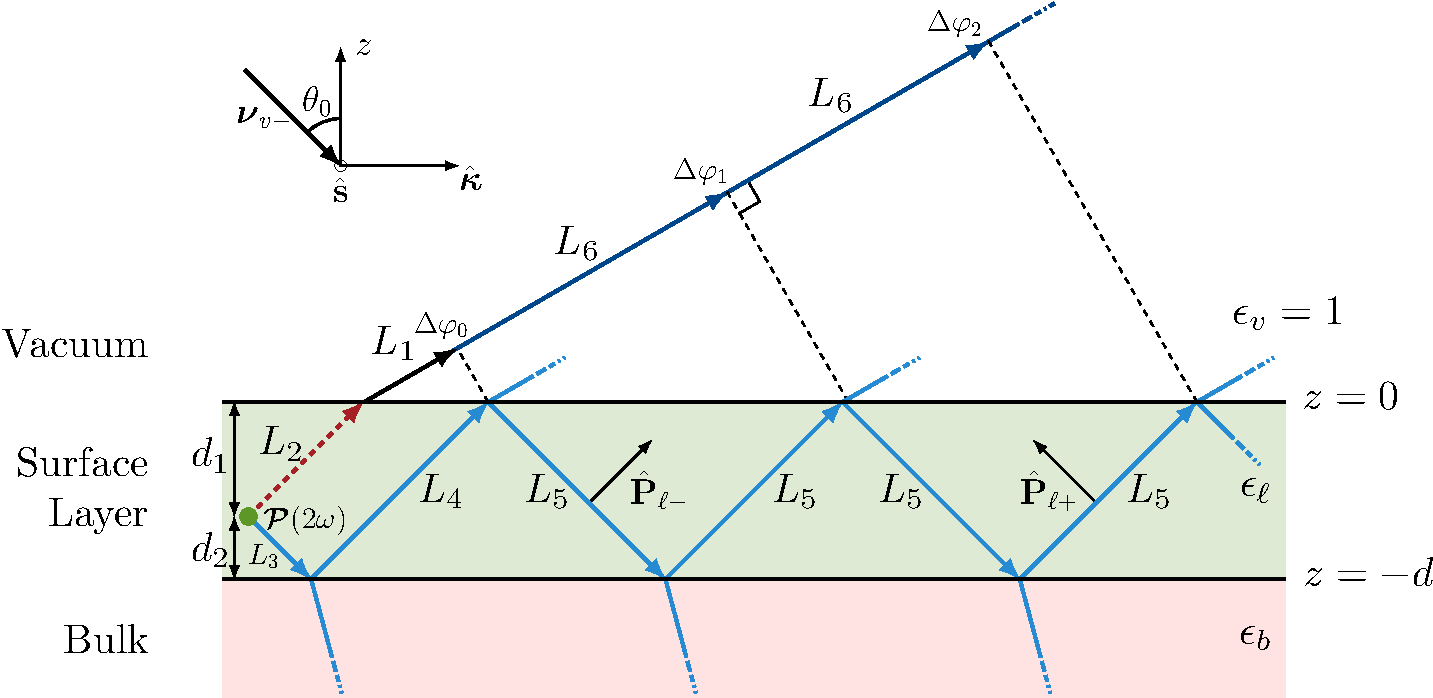
\includegraphics[scale=0.5]{content/figures/diag-3layer_MR_2w}
\caption{Sketch of the three layer model for SHG. The vacuum region ($v$) is on
top with $\epsilon_{v}=1$; the layer $\ell$ of thickness $d = d_{1} + d_{2}$, is
characterized with $\epsilon_{\ell}(\omega)$, and it is where the SH
polarization sheet $\boldsymbol{\mathcal{P}}_{\ell}(2\omega)$ is located at
$z_{\ell} = d_{1}$. The bulk $b$ is described with $\epsilon_{b}(\omega)$. The
arrows point along the direction of propagation, and the $p$-polarization unit
vector, $\hat{\mathbf{P}}_{\ell -(+)}$, along the downward (upward) direction is
denoted with a thick arrow. The $s$-polarization unit vector $\hat{\mathbf{s}}$,
points out of the page. The fundamental field $\mathbf{E}(\omega)$ is incident
from the vacuum side along the $\hat{\boldsymbol{\kappa}z}$-plane, with
$\theta_{0}$ its angle of incidence and $\boldsymbol{\nu}_{v-}$ its wave vector.
$\Delta\varphi_{i}$ denote the phase difference of the multiple reflected beams
with respect to the first vacuum transmitted beam (dashed-red arrow), where the
dotted lines are perpendicular to this beam.}
\label{fig:MR3layer2w}
\end{figure}

From Fig. \ref{fig:MR3layer2w}, we observe the propagation of the SH field as it
is refracted at the layer-vacuum interface ($\ell v$), and  reflected multiple
times from the layer-bulk ($\ell b$) and layer-vacuum ($\ell v$) interfaces.
Thus, we can define
\begin{equation}\label{eq:r5}
\mathbf{T}^{\ell v}
= \hat{\mathbf{s}}T_{s}^{\ell v}\hat{\mathbf{s}} 
+ \hat{\mathbf{P}}_{v+}T_{p}^{\ell v} \hat{\mathbf{P}}_{\ell +},
\end{equation}
as the transmission tensor for the $\ell v$ interface,
\begin{equation}\label{eq:r6}
\mathbf{R}^{\ell b}
= \hat{\mathbf{s}}R_{s}^{\ell b}\hat{\mathbf{s}}
+ \hat{\mathbf{P}}_{\ell +}R_{p}^{\ell b} \hat{\mathbf{P}}_{\ell -},
\end{equation} 
as the reflection tensor for the $\ell b$ interface, and
\begin{equation}\label{eq:r6b}
\mathbf{R}^{\ell v}
= \hat{\mathbf{s}}R_{s}^{\ell v}\hat{\mathbf{s}}
+ \hat{\mathbf{P}}_{\ell -}R_{p}^{\ell v} \hat{\mathbf{P}}_{\ell +},
\end{equation} 
as the reflection tensor for the $\ell v$ interface. The Fresnel factors in
uppercase letters, $T^{ij}_{s,p}$ and $R^{ij}_{s,p}$, are evaluated at $2\omega$
from the following well known formulas
\begin{equation}\label{eq:e.f1}
\begin{split}
t_{s}^{ij}(\omega) &=
\frac{2w_{i}(\omega)}{w_{i}(\omega) + w_{j}(\omega)},
\quad\quad  
t_{p}^{ij}(\omega) =
\frac{2w_{i}(\omega)\sqrt{\epsilon_{i}(\omega)\epsilon_j(\omega)}}
     {w_{i}(\omega)\epsilon_{j}(\omega) + w_{j}(\omega)\epsilon_{i}(\omega)},\\
r_{s}^{ij}(\omega) &=
\frac{w_{i}(\omega) - w_{j}(\omega)}
     {w_{i}(\omega) + w_{j}(\omega)},
\quad\quad 
r_{p}^{ij}(\omega) =
\frac{w_{i}(\omega)\epsilon_{j}(\omega) - w_{j}\epsilon_{i}(\omega)}
     {w_{i}(\omega)\epsilon_{j}(\omega) + w_{j}(\omega)\epsilon_{i}(\omega)}. 
\end{split}
\end{equation}
With these expressions we easily derive the following useful relations,
\begin{equation}\label{eq:mf}
\begin{split}
1 + r^{\ell b}_{s} &= t^{\ell b}_{s},\\
1 + r^{\ell b}_{p} &= \frac{n_{b}}{n_{\ell}}t^{\ell b}_{p},\\
1 - r^{\ell b}_{p} &= \frac{n_{\ell}}{n_{b}}\frac{w_{b}}{w_{\ell}}
                      t^{\ell b}_{p},\\
t^{\ell v}_{p} &= \frac{w_{\ell}}{w_{v}}t^{v\ell}_{p},\\
t^{\ell v}_{s} &= \frac{w_{\ell}}{w_{v}}t^{v\ell}_{s}.
\end{split}
\end{equation}


%%%%%%%%%%%%%%%%%%%%%%%%%%%%%%%%%%%%%%%%%%%%%%%%%%%%%%%%%%%%%%%%%%%%%%%%%%%%%%%%

\subsection{Multiple SHG reflections}

The SH field $\mathbf{E}(2\omega)$ radiated by the SH polarization
$\boldsymbol{\mathcal{P}}_{\ell}(2\omega)$ will radiate directly into the vacuum
and the bulk, where it will be reflected back at the layer-bulk interface into
the thin layer. This beam will be transmitted and reflected multiple times, as
shown in Fig. \ref{fig:MR3layer2w}. As the two beams propagate, a phase
difference will develop between them according to
\begin{equation}\label{eq:m99}
\begin{split}
\Delta\varphi_{m} 
&= \tilde{\Omega}
\Big(
(L_{3} + L_{4} + 2mL_{5})N_{\ell}
 - \big(L_{2}N_{\ell} + (L_{1} + mL_{6})N_{v}\big)
\Big)\\
&= \delta_{0} + m\delta\quad m=0,1,2,\ldots,
\end{split}
\end{equation}
where
\begin{equation}\label{eq:delta0}
\delta_{0} =
8\pi\left(\frac{d_{2}}{\lambda_{0}}\right)W_{\ell},
\end{equation}
and
\begin{equation}\label{eq:delta}
\delta = 8\pi
\left(\frac{d}{\lambda_{0}}\right)W_{\ell},
\end{equation}
where $\lambda_{0}$ is the wavelength of the fundamental field in the vacuum,
$d$ is the thickness of layer $\ell$, and $d_{2}$ is the distance of
$\boldsymbol{\mathcal{P}}_{\ell}(2\omega)$ from the $\ell b$ interface (see Fig.
\ref{fig:MR3layer2w}). We see that $\delta_{0}$ is the phase difference of the
first and second transmitted beams, and $m\delta$ that of the first and third
($m = 1$), first and fourth ($m = 2$), and so on. Note that the thickness $d$ of
the layer $\ell$ enters through the phase $\delta$, and the position $d_{2}$ of
the nonlinear polarization sheet $\mathbf{P}(\mathbf{r},t)$ (Eq.
\eqref{eq:psheet}) enters through $\delta_{0}$. In particular, $d_{2}$ could be
used as a variable to study the effects of multiple reflections on the SSHG
yield $\mathcal{R}(2\omega)$.

To take into account the multiple reflections of the generated SH field in the
layer $\ell$, we proceed as follows. I include the algebra for the $p$-polarized
SH field, and the $s$-polarized field could be worked out along the same steps.
The $p$-polarized $\mathbf{E}_{\ell,p}(2\omega)$ field reflected multiple times
is given by
\begin{equation}\label{eq:E2wcomplete}
\begin{split}
\mathbf{E}_{\ell,p}(2\omega) 
&= E_{\ell,p+}(2\omega)\mathbf{T}^{\ell v}\cdot\hat{\mathbf{P}}_{\ell +}
 + E_{\ell,p-}(2\omega)\mathbf{T}^{\ell v}
\cdot\mathbf{R}^{\ell b}\cdot\hat{\mathbf{P}}_{\ell-}e^{i\Delta\varphi_{0}}\\
&+ E_{\ell,p-}(2\omega)\mathbf{T}^{\ell v}
\cdot\mathbf{R}^{\ell b}\cdot\mathbf{R}^{\ell v}
\cdot\mathbf{R}^{\ell b}\cdot\hat{\mathbf{P}}_{\ell-}e^{i\Delta\varphi_{1}}
\\
&+ E_{\ell,p-}(2\omega)\mathbf{T}^{\ell v}
\cdot\mathbf{R}^{\ell b}\cdot\mathbf{R}^{\ell v}
\cdot\mathbf{R}^{\ell b}\cdot\mathbf{R}^{\ell v}
\cdot\mathbf{R}^{\ell b}\cdot\hat{\mathbf{P}}_{\ell-}e^{i\Delta\varphi_{2}}
+\cdots\\
&= E_{\ell,p+}(2\omega)\mathbf{T}^{\ell v}\cdot\hat{\mathbf{P}}_{\ell +}
+ E_{\ell,p-}(2\omega) \mathbf{T}^{\ell v}
\cdot\sum_{m=0}^\infty  
\big(
\mathbf{R}^{\ell b}\cdot\mathbf{R}^{\ell v} 
e^{i\delta}\Big)^m 
\cdot\mathbf{R}^{\ell b}\cdot\hat{\mathbf{P}}_{\ell-}e^{i\delta_{0}}.
\end{split}
\end{equation}
From Eqs. \eqref{eq:r5} - \eqref{eq:r6b} it is easy to show that
\begin{equation*}\label{eq:m1}
\mathbf{T}^{\ell v}\cdot
\Big(\mathbf{R}^{\ell b}\cdot\mathbf{R}^{\ell v}\Big)^{n}\cdot
\mathbf{R}^{\ell b}
= \hat{\mathbf{s}}T^{\ell v}_{s}
  \Big(R^{\ell b}_{s}R^{\ell v}_{s}\Big)^{n}R^{\ell b}_{s}\hat{\mathbf{s}}
+ \hat{\mathbf{P}}_{v+}T^{\ell v}_{p}\Big(R^{\ell b}_{p}R^{\ell v}_{p}\Big)^n 
  R^{\ell b}_{p} 
\hat{\mathbf{P}}_{\ell-},
\end{equation*}
then,
\begin{equation}\label{eq:E2wreduced}
\mathbf{E}_{\ell,p}(2\omega) 
= \hat{\mathbf{P}}_{\ell +}T^{\ell v}_{p}
\Big(
E_{\ell,p+}(2\omega) +
\frac{R^{\ell b}_{p}e^{i\delta_{0}}}{1 + R^{v\ell}_{p}R^{\ell b}_{p}e^{i\delta}}
E_{\ell,p-}(2\omega) 
\Big),
\end{equation}
where we used $R^{ij}_{s,p} = -R^{ji}_{s,p}$. Using Eq. \eqref{eq:solmaxwell}
and \eqref{eq:mf}, we can readily write
\begin{equation}\label{eq:mr8}
\mathbf{E}_{\ell,p}(2\omega) =
\frac{\gamma i\tilde{\Omega}}{W_{\ell}}\mathbf{H}_{\ell}\cdot
\boldsymbol{\mathcal{P}}_{\ell}(2\omega),
\end{equation}
where
\begin{equation}\label{eq:mr9}
\mathbf{H}_{\ell}
= \frac{W_\ell}{W_v}
\left[
\hat{\mathbf{s}}\,T_{s}^{v\ell}
\left(1+ R^{M}_{s}\right)\hat{\mathbf{s}} + \hat{\mathbf{P}}_{v+}T_{p}^{v\ell}
\left(\hat{\mathbf{P}}_{\ell +} + R^{M}_{p}\hat{\mathbf{P}}_{\ell -}\right)
\right],
\end{equation}
and
\begin{equation}\label{m61}
R^{M}_{\mathrm{i}}\equiv
\frac{R^{\ell b}_{\mathrm{i}}e^{i\delta_{0}}}
     {1+R^{v\ell}_{\mathrm{i}} R^{\ell b}_{\mathrm{i}}e^{i\delta}},
     \quad \mathrm{i}=s,p,
\end{equation}
is defined as the multiple ($M$) reflection coefficient. This coefficient
depends on the thickness $d$ of layer $\ell$, and most importantly on the
position $d_{2}$ of $\boldsymbol{\mathcal{P}}_{\ell}(2\omega)$ within this
layer. The final results will depend on both $d$ and $d_{2}$. However, we can
also define an average $\bar{R}^{M}_{\mathrm{i}}$ as
\begin{equation}\label{eq:mcave}
\bar{R}^{M}_{\mathrm{i}}\equiv 
\frac{1}{d}\int_{0}^{d}R^{M}_{\mathrm{i}}(x)\,dx\propto
\frac{1}{d}\int_{0}^{d}e^{i\alpha x}\,dx,
\end{equation}
where
\begin{equation}\label{eq:m16}
R^{M}_{\mathrm{i}}(x) = 
\frac{R^{\ell b}_{\mathrm{i}}e^{i\alpha x}}
{1 + R^{v\ell}_{\mathrm{i}}R^{\ell b}_{\mathrm{i}}e^{i\delta}},
\end{equation}
and $\alpha=8\pi W_{\ell}/\lambda_{0}$. We can evaluate the rightmost integral,
\begin{align}\label{eq:integral}
\frac{1}{d}\int_{0}^{d} e^{i\alpha x}\,dx
&= \frac{1}{d}\frac{e^{i\alpha x}}{i\alpha}\,\Bigg\vert^{d}_{0}
 = \frac{1}{i\alpha d}\left(e^{i\alpha d} - 1\right)\nonumber\\\nonumber\\
&= \frac{1}{i\delta}\left(e^{i\delta} - 1\right)
 = \frac{1}{i\delta}e^{i\delta/2}\frac{(e^{i\delta/2} - e^{-i\delta/2})}{2i}
 = e^{i\delta/2}\,\mathrm{sinc}(\delta/2).
\end{align}
Therefore, we can establish the average value $\bar{R}^{M}_{\mathrm{i}}$ as
\begin{align}\label{eq:mcave2}
\bar{R}^{M}_{\mathrm{i}} = 
\frac{R^{\ell b}_{\mathrm{i}}e^{i\delta/2}}
{1 + R^{v\ell}_{\mathrm{i}}R^{\ell b}_{\mathrm{i}}e^{i\delta}}
\,\mathrm{sinc}(\delta/2),
\end{align}
that only depends on $d$ through the $\delta$ term from Eq. \eqref{eq:delta}.

To connect with the work in Ref. \cite{mizrahiJOSA88}, where
$\boldsymbol{\mathcal{P}}(2\omega)$ is located on top of the vacuum-surface
interface and only the vacuum radiated beam and the first (and only) reflected
beam need be considered, we take $\ell = v$ and $d_{2} = 0$, then $T^{\ell v} =
1$, $R^{v\ell} = 0$ and $\delta_{0} = 0$, with which $R^{M}_{\mathrm{i}} =
R^{vb}_{\mathrm{i}}$. Thus, Eq. \eqref{eq:mr9} coincides with Eq. (3.8) of Ref.
\cite{mizrahiJOSA88}.


%%%%%%%%%%%%%%%%%%%%%%%%%%%%%%%%%%%%%%%%%%%%%%%%%%%%%%%%%%%%%%%%%%%%%%%%%%%%%%%%

\subsection{Multiple reflections for the linear field}

For a more complete formulation, we must also consider the multiple reflections
of the fundamental field $\mathbf{E}_{\ell}(\omega)$ inside the thin $\ell$
layer. In Fig. \ref{fig:MR3layer1w} I present the situation where
$\mathbf{E}_{v}(\omega)$ impinges from the vacuum side with an angle of
incidence $\theta_{0}$. As the first transmitted beam is multiply reflected from
the $\ell b$ and the $\ell v$ interfaces, it accumulates a phase difference of
$n\phi$, with $n=1,2,3,\ldots$, given by
\begin{equation}\label{mphi}
\begin{split}
\varphi &= \frac{\omega}{c}(2L_{1}n_{\ell} - L_{2}n_{v})\\
&= 4\pi\left(\frac{d}{\lambda_{0}}\right)w_{\ell},
\end{split}
\end{equation}
where $n_{v}=1$. Besides the equivalent of Eqs. \eqref{eq:r6} and \eqref{eq:r6b}
for $\omega$, we also need
\begin{equation}\label{eq:mvv}
\mathbf{t}^{v\ell}
= \hat{\mathbf{s}}t_{s}^{v\ell}\hat{\mathbf{s}} 
+ \hat{\mathbf{p}}_{\ell -}t_{p}^{v\ell}\hat{\mathbf{p}}_{v-},
\end{equation}
to write
\begin{align}\label{eq:mcvew}
\mathbf{E}(\omega)
&= E_{0}
\Big[
\mathbf{t}^{v\ell} + \mathbf{r}^{\ell b}\cdot\mathbf{t}^{v\ell}e^{i\varphi}
 + \mathbf{r}^{\ell b}\cdot\mathbf{r}^{\ell v}\cdot
   \mathbf{r}^{\ell b}\cdot\mathbf{t}^{v\ell} e^{i2\varphi}
 + \mathbf{r}^{\ell b}\cdot\mathbf{r}^{\ell v}\cdot
   \mathbf{r}^{\ell b}\cdot\mathbf{r}^{\ell v}\cdot
   \mathbf{r}^{\ell b}\cdot\mathbf{t}^{v\ell} e^{i3\varphi}
 + \cdots
\Big]\cdot\hat{\mathbf{e}}^{\mathrm{i}}\nonumber\\
&= E_{0}
\Big[
1 + \Big(1 + \mathbf{r}^{\ell b}\cdot\mathbf{r}^{\ell v}e^{i\varphi}
+ (\mathbf{r}^{\ell b}\cdot\mathbf{r}^{\ell v})^2e^{i2\varphi}+\cdots\Big)\cdot
\mathbf{r}^{\ell b}e^{i\varphi}
\Big]
\cdot\mathbf{t}^{v\ell}\cdot\hat{\mathbf{e}}^{\mathrm{i}}\nonumber\\
&= E_{0}
\Big[
\hat{\mathbf{s}} t^{v\ell}_{s}(1+r^{M}_{s})\hat{\mathbf{s}} 
+ t^{v\ell}_{p}
\left(\hat{\mathbf{p}}_{\ell-}+\hat{\mathbf{p}}_{\ell+}r^{M}_{p}\right)
\hat{\mathbf{p}}_{v-}
\Big]\cdot\hat{\mathbf{e}}^{\mathrm{i}},
\end{align}
where $E_{0}$ is the intensity of the fundamental field, and
$\hat{\mathbf{e}}^{\mathrm{i}}$ is the unit vector of the incoming polarization,
with $\mathrm{i} = s,p$, and then, $\hat{\mathbf{e}}^{s}=\hat{\mathbf{s}}$ and
$\hat{\mathbf{e}}^{p}=\hat{\mathbf{p}}_{v-}$. Also,
\begin{equation}\label{mvrm}
r^{M}_{\mathrm{i}} \equiv
\frac{r^{\ell b}_{\mathrm{i}}e^{i\varphi}}{1+r^{v\ell}_{\mathrm{i}}r^{\ell b}_{\mathrm{i}}e^{i\varphi}}, \quad \mathrm{i}=s,p.
\end{equation}
$r^{M}_{\mathrm{i}}$ is defined as the multiple (M) reflection coefficient for
the fundamental field. We define $\mathbf{E}^{\mathrm{i}}_{\ell}(\omega)\equiv
E_{0}\mathbf{e}^{\omega,\mathrm{i}}_{\ell}$ ($\mathrm{i}=s,p$), where
\begin{equation}\label{eq:mcvew2}
\mathbf{e}^{\omega,\mathrm{i}}_\ell 
= \Big[\hat{\mathbf{s}} t^{v\ell}_s(1+r^M_s)\hat{\mathbf{s}} 
+ t^{v\ell}_p\left(\hat{\mathbf{p}}_{\ell-}+\hat{\mathbf{p}}_{\ell+}r^{M}_p 
\right)\hat{\mathbf{p}}_{v-}
\Big]\cdot\hat{\mathbf{e}}^{\mathrm{i}},
\end{equation}
and using Eq. \eqref{eq:r4} we obtain that
\begin{equation}\label{eq:mcvep}
\mathbf{e}^{\omega,p}_{\ell}=\frac{t^{v\ell}_{p}}{n_{\ell}}
\left( 
  r^{M+}_{p}\sin\theta_{0}\hat{\mathbf{z}}
+ r^{M-}_{p}w_{\ell}\hat{\boldsymbol{\kappa}}
\right),
\end{equation} 
for $p$-input polarization with
$\hat{\mathbf{e}}^{\mathrm{i}}=\hat{\mathbf{p}}_{v-}$, and
\begin{equation}\label{eq:mcves}
\mathbf{e}^{\omega,s}_\ell=t^{v\ell}_{s}r^{M+}_{s}\hat{\mathbf{s}},
\end{equation}
for $s$-input polarization with
$\hat{\mathbf{e}}^{\mathrm{i}}=\hat{\mathbf{s}}$, where
\begin{equation}\label{eq:mvc}
r^{M\pm}_{\mathrm{i}}=1\pm r^{M}_{\mathrm{i}},\quad \mathrm{i} = s,p.
\end{equation}

\begin{figure}
\centering 
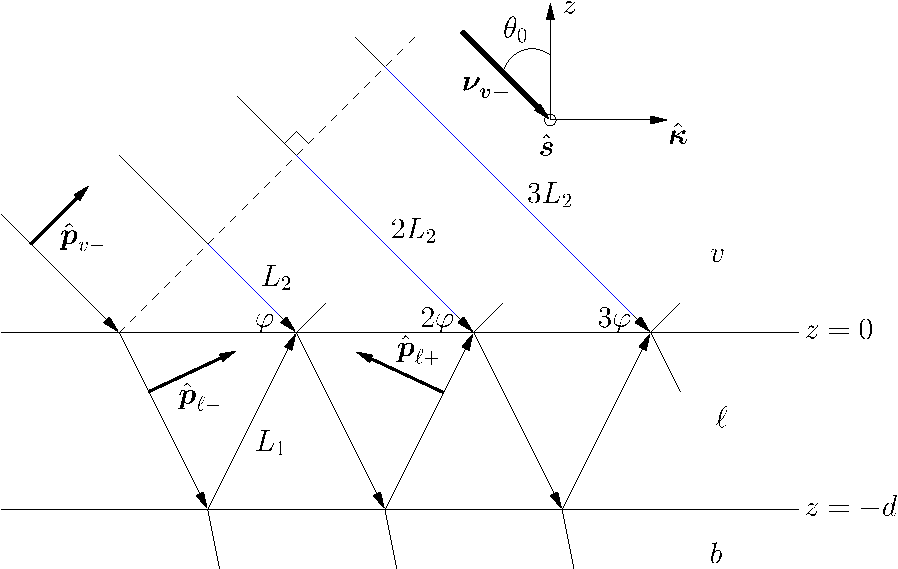
\includegraphics[scale=0.6]{content/figures/diag-3layer_MR_1w}
\caption{Sketch for the multiple reflected fundamental field
$\mathbf{E}(\omega)$, which impinges from the vacuum side along the
$\hat{\boldsymbol{\kappa}}z$-plane. $\theta_{0}$ and $\boldsymbol{\nu}_{v-}$ are
the angle of incidence and wave vector, respectively. The arrows point along the
direction of propagation. The $p$-polarization unit vectors
$\hat{\mathbf{p}}_{\beta\pm}$, point along the downward $(-)$ or upward $(+)$
directions and are denoted with thick arrows, where $\beta = v$ or $\ell$. The
$s$-polarization unit vector $\hat{\mathbf{s}}$ points out of the page.
$(1,2,3,\ldots)\varphi$ denotes the phase difference for the multiple reflected
beams with respect to the incident field, where the dotted line is perpendicular
to this beam.}
\label{fig:MR3layer1w}
\end{figure}


%%%%%%%%%%%%%%%%%%%%%%%%%%%%%%%%%%%%%%%%%%%%%%%%%%%%%%%%%%%%%%%%%%%%%%%%%%%%%%%%

\subsection{Deriving the SSHG yield}

The magnitude of the radiated field is given by $E(2\omega) =
\hat{\mathbf{e}}^{\mathrm{F}}\cdot\mathbf{E}_{\ell}(2\omega)$, where
$\hat{\mathbf{e}}^{\mathrm{F}}$ is the unit vector of the final polarization
with $\mathrm{F}=S,P$, where $\hat{\mathbf{e}}^S=\hat{\mathbf{s}}$ and
$\hat{\mathbf{e}}^P=\hat{\mathbf{P}}_{v+}$. We expand the rightmost term in
parenthesis of Eq. \eqref{eq:mr9} as
\begin{equation}
\begin{split}
\hat{\mathbf{P}}_{\ell +} + R^{M}_{p}\hat{\mathbf{P}}_{\ell -}
&= \frac{\sin\theta_{0}\hat{\mathbf{z}} - W_{\ell}\hat{\boldsymbol{\kappa}}}
        {N_{\ell}}
 + R^{M}_{p}
   \frac{\sin\theta_{0}\hat{\mathbf{z}} + W_{\ell}\hat{\boldsymbol{\kappa}}}
        {N_{\ell}}\\
&= \frac{1}{N_{\ell}}
\left(
\sin\theta_{0}R^{M+}_{p}\hat{\mathbf{z}}
- W_{\ell}R^{M-}_{p}\hat{\boldsymbol{\kappa}}
\right),
\end{split}
\end{equation}
where
\begin{equation}\label{eq:rm}
R^{M\pm}_{\mathrm{i}}\equiv 1 \pm R^{M}_{\mathrm{i}}, \quad \mathrm{i}=s,p.
\end{equation}
Using Eq. \eqref{eq:mf} we write Eq. \eqref{eq:mr8} as
\begin{equation}\label{eq:r10}
E(2\omega) = \frac{2\gamma i\omega}{cW_\ell}
\hat{\mathbf{e}}^{\mathrm{F}}\cdot\mathbf{H}_{\ell}\cdot
\boldsymbol{\mathcal{P}}_{\ell}(2\omega) 
= \frac{2\gamma i\omega}{cW_{v}}
\mathbf{e}^{\,2\omega,\mathrm{F}}_{\ell}\cdot
\boldsymbol{\mathcal{P}}_{\ell}(2\omega),
\end{equation}
where
\begin{equation}\label{eq:r12mm}
\mathbf{e}^{2\omega,\mathrm{F}}_{\ell} =\hat{\mathbf{e}}^{\mathrm{F}}\cdot 
\Bigg[
\hat{\mathbf{s}}T_{s}^{v\ell}R^{M+}_{s}\hat{\mathbf{s}} + 
\hat{\mathbf{P}}_{v+}
\frac{T^{v\ell}_{p}}
     {N_{\ell}}
\left(
\sin\theta_{0}R^{M+}_{p}\hat{\mathbf{z}}
- W_{\ell}R^{M-}_{p}\hat{\boldsymbol{\kappa}}
\right) 
\Bigg]. 
\end{equation}  
Replacing $\mathbf{E}(\omega)\to E_0\mathbf{e}^{\omega,\mathrm{i}}_\ell$, in Eq.
\eqref{eq:tres}, we obtain that
\begin{equation}\label{eq:m4}
\boldsymbol{\mathcal{P}}_{\ell}(2\omega) = 
\left\{
\begin{array}{cc}  
E^{2}_{0}\,
\boldsymbol{\chi}:\mathbf{e}^{\omega,\mathrm{i}}_{\ell}
                  \mathbf{e}^{\omega,\mathrm{i}}_{\ell}
& \text{(CGS units)}\\\\
\epsilon_{0}E^{2}_{0}\,
\boldsymbol{\chi}:\mathbf{e}^{\omega,\mathrm{i}}_{\ell}
                  \mathbf{e}^{\omega,\mathrm{i}}_{\ell}
& \text{(MKS units)}\\
\end{array}
\right.,
\end{equation}
where $\mathbf{e}^{\omega,\mathrm{i}}_{\ell}$ is given by Eq. \eqref{eq:mcvew2},
and thus Eq. \eqref{eq:r10} reduces to ($W_{v}=\cos\theta_{0}$)
\begin{equation}\label{eq:mr10}
E_{\ell}(2\omega) 
= \frac{2\eta i \omega}{c\cos\theta_{0}}
\mathbf{e}^{2\omega,\mathrm{F}}_{\ell}\cdot
\boldsymbol{\chi}:\mathbf{e}^{\omega,\mathrm{i}}_{\ell}
                  \mathbf{e}^{\omega,\mathrm{i}}_{\ell},
\end{equation}
where $\eta=2\pi$ in CGS units and $\eta=1/2$ in MKS units. For ease of
notation, we define
\begin{align}\label{eq:mc0}
\Upsilon_{\mathrm{iF}}
\equiv 
\mathbf{e}^{2\omega,\mathrm{F}}_{\ell}\cdot
\boldsymbol{\chi}:\mathbf{e}^{\omega,\mathrm{i}}_{\ell}
                  \mathbf{e}^{\omega,\mathrm{i}}_{\ell},
\end{align}
where i stands for the incoming polarization of the fundamental electric field
given by $\hat{\mathbf{e}}^{\mathrm{i}}$ in Eq. \eqref{eq:mcvew2}, and F for the
outgoing polarization of the SH electric field given by
$\hat{\mathbf{e}}^{\mathrm{F}}$ in Eq. \eqref{eq:r12mm}. I purposely omitted the
full $\boldsymbol{\chi}(-2\omega;\omega,\omega)$ notation, and will do so from
this point on.

From Eqs. \eqref{eq:rintensities} and \eqref{eq:intensity} we obtain that in
CGS units ($\eta=2\pi$), 
\begin{align}\label{eq:r01}
\vert E(2\omega)\vert^{2} &=
\vert E_{0}\vert^{4}\frac{16\pi^{2}\omega^{2}}{c^{2}W^2_{v}}
\vert\Upsilon_{\mathrm{iF}}\vert^{2}\nonumber\\
%%%%%%%%%%%%%%%%%%%%%%%%%%%%%%%%%%%%%%%%%%%%%%%%%%%%%
\frac{c}{2\pi}\vert\sqrt{N_{v}}E(2\omega)\vert^{2} &=
\frac{32\pi^{3}\omega^{2}}{c^{3}\cos^2\theta_{0}}
\left\vert\frac{\sqrt{N_{v}}}{n^{2}_{\ell}}\Upsilon_{\mathrm{iF}}\right\vert^{2} 
\left(\frac{c}{2\pi}\vert\sqrt{n_{\ell}}E_{0}\vert^{2}\right)^{2}\nonumber\\ 
%%%%%%%%%%%%%%%%%%%%%%%%%%%%%%%%%%%%%%%%%%%%%%%%%%%%%
I(2\omega) &=
\frac{32\pi^{3}\omega^{2}}{c^{3}\cos^2\theta_{0}}
\left\vert\frac{\sqrt{N_{v}}}{n^{2}_{\ell}}\Upsilon_{\mathrm{iF}}\right\vert^{2}
I^{2}(\omega)\nonumber\\
%%%%%%%%%%%%%%%%%%%%%%%%%%%%%%%%%%%%%%%%%%%%%%%%%%%%%
\mathcal{R}_{\mathrm{iF}}(2\omega) &=
\frac{32\pi^{3}\omega^{2}}{c^{3}\cos^2\theta_{0}}
\left\vert\frac{1}{n_{\ell}}\Upsilon_{\mathrm{iF}}\right\vert^{2},
\end{align} 
and in MKS units ($\eta=1/2$),
\begin{align}\label{r01m}
\vert E(2\omega)\vert^{2} &=
\vert E_{0}\vert^{4}\frac{\omega^{2}}{c^{2}W^{2}_{v}}\nonumber\\
%%%%%%%%%%%%%%%%%%%%%%%%%%%%%%%%%%%%%%%%%%%%%%%%%%%%%
2\epsilon_{0}c|\sqrt{N_{v}}E(2\omega)|^{2} &=
\frac{2\epsilon_{0}\omega^{2}}{c\cos^{2}\theta_{0}}
\left\vert\frac{\sqrt{N_{v}}}{n^{2}_{\ell}}\Upsilon_{\mathrm{iF}}\right\vert^{2} 
\frac{1}{4\epsilon^{2}_0c^{2}}
\left(2\epsilon_{0}c\vert\sqrt{n_{\ell}}E_{0}\vert^{2}\right)^{2}\nonumber\\
%%%%%%%%%%%%%%%%%%%%%%%%%%%%%%%%%%%%%%%%%%%%%%%%%%%%%
I(2\omega) &= 
\frac{\omega^{2}}{2\epsilon_{0}c^3\cos^{2}\theta_{0}}
\left\vert\frac{\sqrt{N_{v}}}{n^{2}_{\ell}}\Upsilon_{\mathrm{iF}}\right\vert^{2}
I^{2}(\omega)\nonumber\\
%%%%%%%%%%%%%%%%%%%%%%%%%%%%%%%%%%%%%%%%%%%%%%%%%%%%%
\mathcal{R}_{\mathrm{iF}}(2\omega) &=
\frac{\omega^{2}}{2\epsilon_{0}c^3\cos^{2}\theta_{0}}
\left\vert  \frac{1}{n_{\ell}}\Upsilon_{\mathrm{iF}}\right\vert^{2}.
\end{align}
Finally, we condense these results and establish the SSHG yield as
\begin{equation}\label{eq:mc6}
\mathcal{R}_{\mathrm{iF}}(2\omega) 
\left\{
\begin{array}{ r c } 
\frac{32\pi^{3}\omega^{2}}{c^{3}\cos^{2}\theta_{0}}
\left\vert\frac{1}{n_{\ell}}\Upsilon_{\mathrm{iF}}\right\vert^{2} 
& \text{(CGS units)} \\
\frac{\omega^{2}}{2\epsilon_{0}c^3\cos^{2}\theta_{0}}
\left\vert\frac{1}{n_{\ell}}\Upsilon_{\mathrm{iF}}\right\vert^{2} 
& \text{(MKS units)} 
\end{array}
\right.,
\end{equation}
where $N_{v}=1$ and $W_{v}=\cos\theta_{0}$. In the MKS unit system
$\boldsymbol{\chi}$ is given in m$^{2}$/V, since it is a surface second order
nonlinear susceptibility, and $\mathcal{R}_{\mathrm{iF}}$ is given in m$^2$/W.

I include a full treatise on this exact procedure without considering the
effects of multiple reflections in Appendix \ref{app:shgyieldnomr}.


%%%%%%%%%%%%%%%%%%%%%%%%%%%%%%%%%%%%%%%%%%%%%%%%%%%%%%%%%%%%%%%%%%%%%%%%%%%%%%%%
%%%%%%%%%%%%%%%%%%%%%%%%%%%%%%%%%%%%%%%%%%%%%%%%%%%%%%%%%%%%%%%%%%%%%%%%%%%%%%%%

\section{\texorpdfstring{$\mathcal{R}_{\mathrm{iF}}$}{R} for different
polarization cases}\label{sec:rcases}

We now have everything we need to derive explicit expressions for
$\mathcal{R}_{\mathrm{iF}}$, Eq. \eqref{eq:mc6}, for the most commonly used
polarizations of incoming and outgoing fields (iF=$pP$, $pS$, $sP$, and $sS$).
For this, we must expand $\Upsilon_{\mathrm{iF}}$ from Eq. \eqref{eq:mc0} for
each case. By substituting Eqs. \eqref{eq:mc1} and \eqref{eq:mmc2} into Eq.
\eqref{eq:r12mm}, we obtain
\begin{equation}\label{eq:e2wpmr}
\mathbf{e}^{2\omega,P}_{\ell} =
\frac{T^{v\ell}_{p}}{N_{\ell}}
\big(
  \sin\theta_{0}R^{M+}_{p}\hat{\mathbf{z}}
- W_{\ell}R^{M-}_{p}\cos\phi\hat{\mathbf{x}}
- W_{\ell}R^{M-}_{p}\sin\phi\hat{\mathbf{y}}
\big),
\end{equation}
for $P$ $(\hat{\mathbf{e}}^{\mathrm{F}} = \hat{\mathbf{P}}_{v+})$ outgoing
polarization, and
\begin{equation}\label{eq:e2wsmr}
\mathbf{e}^{2\omega,S}_{\ell} =
T_{s}^{v\ell}R^{M+}_{s}
\left(
- \sin\phi\hat{\mathbf{x}}
+ \cos\phi\hat{\mathbf{y}}
\right).
\end{equation}
for $S$ $(\hat{\mathbf{e}}^{\mathrm{F}}=\hat{\mathbf{s}})$ outgoing
polarization.

Following a similar procedure, we use Eqs. \eqref{eq:mc1} and \eqref{eq:mmc2}
with Eq. \eqref{eq:mcvep}, and obtain
\begin{equation}\label{eq:ewewpmr}
\begin{split}
\mathbf{e}^{\omega,\mathrm{p}}_{\ell}\mathbf{e}^{\omega,\mathrm{p}}_{\ell} =
\left(\frac{t^{v\ell}_{p}}{n_{\ell}}\right)^{2}
\bigg(
  \big(&r^{M-}_{p}\big)^{2}w^{2}_{\ell}\cos^{2}\phi
  \hat{\mathbf{x}}\hat{\mathbf{x}}
+ 2\big(r^{M-}_{p}\big)^{2}w^{2}_{\ell}\sin\phi\cos\phi
  \hat{\mathbf{x}}\hat{\mathbf{y}}\\
+ 2&r^{M+}_{p}r^{M-}_{p}w_{\ell}\sin\theta_{0}\cos\phi
  \hat{\mathbf{x}}\hat{\mathbf{z}}
+ \big(r^{M-}_{p}\big)^{2}w^{2}_{\ell}\sin^{2}\phi
  \hat{\mathbf{y}}\hat{\mathbf{y}}\\
+ 2&r^{M+}_{p}r^{M-}_{p}w_{\ell}\sin\theta_{0}\sin\phi
  \hat{\mathbf{y}}\hat{\mathbf{z}}
+ \big(r^{M+}_{p}\big)^{2}\sin^{2}\theta_{0}
   \hat{\mathbf{z}}\hat{\mathbf{z}}
\bigg),
\end{split}
\end{equation}
for $p$ incoming polarization $(\hat{\mathbf{e}}^{\mathrm{i}} =
\hat{\mathbf{p}}_{v-})$, and with Eq. \eqref{eq:mcves},
\begin{equation}\label{eq:ewewsmr}
\mathbf{e}^{\omega,\mathrm{s}}_{\ell}\mathbf{e}^{\omega,\mathrm{s}}_{\ell}
= \left(t^{v\ell}_{s}r^{M+}_{s}\right)^{2}
\big(
  \sin^{2}\phi\hat{\mathbf{x}}\hat{\mathbf{x}}
 + \cos^{2}\phi\hat{\mathbf{y}}\hat{\mathbf{y}}
 - 2\sin\phi\cos\phi\hat{\mathbf{x}}\hat{\mathbf{y}}
\big).
\end{equation}
for $s$ incoming polarization $(\hat{\mathbf{e}}^{\mathrm{i}} =
\hat{\mathbf{s}})$.

I have summarized the combination of equations needed to derive the expressions
or all four polarization cases of $\mathcal{R}_{\mathrm{iF}}$ in Table
\ref{tab:summary}. In the following subsections we will derive the explicit
expressions for $\Upsilon_{\mathrm{iF}}$ for the most general case where the
surface has no symmetry other than that of noncentrosymmetry. We will then
develop these expressions for particular cases of the most commonly investigated
surfaces, the (111), (001), and (110) crystallographic faces. For ease of
writing we split $\Upsilon_{\mathrm{iF}}$ as
\begin{equation}\label{eq:mc25}
\Upsilon_{\mathrm{iF}} = \Gamma_{\mathrm{iF}}\,r_{\mathrm{iF}}.
\end{equation} 

Lastly, in Table \ref{tab:chis} I list the nonzero components of
$\boldsymbol{\chi}$ for each surface symmetry \cite{sipePRB87, popovbook}.

\begin{table}
\centering
\begin{tabular}{| c | l | l | c | c |}
\hline
Case               & $\hat{\mathbf{e}}^{\mathrm{F}}$
                   & $\hat{\mathbf{e}}^{\mathrm{i}}$
                   & $\mathbf{e}^{2\omega,\mathrm{F}}_{\ell}$
                   & $\mathbf{e}^{\omega,\mathrm{i}}_{\ell}
                      \mathbf{e}^{\omega,\mathrm{i}}_{\ell}$ \\
\hline
$\mathcal{R}_{pP}$ & $\hat{\mathbf{P}}_{v+}$
                   & $\hat{\mathbf{p}}_{v-}$
                   &  Eq. \eqref{eq:e2wpmr} & Eq. \eqref{eq:ewewpmr} \\
$\mathcal{R}_{pS}$ & $\hat{\mathbf{S}}$
                   & $\hat{\mathbf{p}}_{v-}$
                   &  Eq. \eqref{eq:e2wsmr} & Eq. \eqref{eq:ewewpmr} \\
$\mathcal{R}_{sP}$ & $\hat{\mathbf{P}}_{v+}$
                   & $\hat{\mathbf{s}}$
                   &  Eq. \eqref{eq:e2wpmr} & Eq. \eqref{eq:ewewsmr} \\
$\mathcal{R}_{sS}$ & $\hat{\mathbf{S}}$
                   & $\hat{\mathbf{s}}$
                   &  Eq. \eqref{eq:e2wsmr} & Eq. \eqref{eq:ewewsmr} \\
\hline
\end{tabular}
\caption{Polarization unit vectors for $\hat{\mathbf{e}}^{\mathrm{F}}$ and
$\hat{\mathbf{e}}^{\mathrm{i}}$, and equations describing
$\mathbf{e}^{2\omega,\mathrm{F}}_{\ell}$ and
$\mathbf{e}^{\omega,\mathrm{i}}_{\ell}\mathbf{e}^{\omega,\mathrm{i}}_{\ell}$ for
each polarization case.}
\label{tab:summary}
\end{table}

\begin{table}
\centering
\begin{tabular}{| c | c | c |}
\hline 
(111)-$C_{3v}$     & (110)-$C_{2v}$  & (001)-$C_{4v}$ \\
\hline 
$\chi^{zzz}$ & $\chi^{zzz}$ & $\chi^{zzz}$\\
$\chi^{zxx}=\chi^{zyy}$ & $\chi^{zxx}\ne\chi^{zyy}$ & $\chi^{zxx}=\chi^{zyy}$\\
$\chi^{xxz}=\chi^{yyz}$ & $\chi^{xxz}\ne\chi^{yyz}$ & $\chi^{xxz}=\chi^{yyz}$\\
$\chi^{xxx}=-\chi^{xyy}=-\chi^{yyx}$ & &  \\
\hline 
\end{tabular}
\caption{Components of $\boldsymbol{\chi}$ for the (111), (110) and (001)
crystallographic faces, belonging to the $C_{3v}$, $C_{2v}$, and $C_{4v}$,
symmetry groups, respectively. For the (111) surface we choose the $x$ and $y$
axes along the [$11\bar{2}$] and [$1\bar{1}0$] directions, respectively. For the
(110) and (001) we consider the $y$ axis perpendicular to the plane of
symmetry.\cite{sipePRB87} We remark that in general
$\boldsymbol{\chi}^{(111)}\ne \boldsymbol{\chi}^{(110)} \ne
\boldsymbol{\chi}^{(001)}$.}
\label{tab:chis}
\end{table}

I have provided the full, step-by-step derivation for all of these expressions
in Appendix \ref{app:sshg_explicit_expressions_rif}, with and without the
effects of multiple reflections. The avid reader should refer to that chapter if
interested in deriving any of the expressions listed below.


%%%%%%%%%%%%%%%%%%%%%%%%%%%%%%%%%%%%%%%%%%%%%%%%%%%%%%%%%%%%%%%%%%%%%%%%%%%%%%%%

\subsection{\texorpdfstring{$\mathcal{R}_{pP}$ ($p$-in, $P$-out)}
{RpP (p-in, P-out)}}
\label{sec:RpP} 

Per Table \ref{tab:summary}, $\mathcal{R}_{pP}$ requires Eqs. \eqref{eq:e2wpmr}
and \eqref{eq:ewewpmr}. After some algebra, we obtain that
\begin{equation}\label{eq:mc78}
\Gamma_{pP} =
\frac{T^{v\ell}_{p}}{N_{\ell}}
\left(\frac{t^{v\ell}_{p}}{n_{\ell}}\right)^{2}
,
\end{equation}
and
\begin{equation}
\begin{split}
r_{pP} =
&-R^{M-}_{p}\left(r^{M-}_{p}\right)^{2}w^{2}_{\ell}W_{\ell}\cos^{3}\phi
\chi^{xxx}
 -2R^{M-}_{p}\left(r^{M-}_{p}\right)^{2}w^{2}_{\ell}W_{\ell}\sin\phi\cos^{2}\phi
\chi^{xxy}\\
&-2R^{M-}_{p}r^{M+}_{p}r^{M-}_{p}w_{\ell}W_{\ell}\sin\theta_{0}\cos^{2}\phi
\chi^{xxz}
 -R^{M-}_{p}\left(r^{M-}_{p}\right)^{2}w^{2}_{\ell}W_{\ell}\sin^{2}\phi\cos\phi
\chi^{xyy}\\
&-2R^{M-}_{p}r^{M+}_{p}r^{M-}_{p}w_{\ell}W_{\ell}\sin\theta_{0}\sin\phi\cos\phi
\chi^{xyz}
 -R^{M-}_{p}\left(r^{M+}_{p}\right)^{2}W_{\ell}\sin^{2}\theta_{0}\cos\phi
\chi^{xzz}\\
%%%%%%%%%%%%%%%%%%%%%%%%%%%%%%%%%%%%%%%%%%%%%%%%%%%%%%%%%%%%
&-R^{M-}_{p}\left(r^{M-}_{p}\right)^{2}w^{2}_{\ell}W_{\ell}\sin\phi\cos^{2}\phi
\chi^{yxx}
 -2R^{M-}_{p}\left(r^{M-}_{p}\right)^{2}w^{2}_{\ell}W_{\ell}\sin^{2}\phi\cos\phi
\chi^{yxy}\\
&-2R^{M-}_{p}r^{M+}_{p}r^{M-}_{p}w_{\ell}W_{\ell}\sin\theta_{0}\sin\phi\cos\phi
\chi^{yxz}
 -R^{M-}_{p}\left(r^{M-}_{p}\right)^{2}w^{2}_{\ell}W_{\ell}\sin^{3}\phi
\chi^{yyy}\\
&-2R^{M-}_{p}r^{M+}_{p}r^{M-}_{p}w_{\ell}W_{\ell}\sin\theta_{0}\sin^{2}\phi
\chi^{yyz}
 -R^{M-}_{p}\left(r^{M+}_{p}\right)^{2}W_{\ell}\sin^{2}\theta_{0}\sin\phi
\chi^{yzz}\\
%%%%%%%%%%%%%%%%%%%%%%%%%%%%%%%%%%%%%%%%%%%%%%%%%%%%%%%%%%%%
&+R^{M+}_{p}\left(r^{M-}_{p}\right)^{2}w^{2}_{\ell}\sin\theta_{0}\cos^{2}\phi
\chi^{zxx}
 +2R^{M+}_{p}r^{M+}_{p}r^{M-}_{p}w_{\ell}\sin^{2}\theta_{0}\cos\phi
\chi^{zxz}\\
&+2R^{M+}_{p}\left(r^{M-}_{p}\right)^{2}w^{2}_{\ell}\sin\theta_{0}\sin\phi
\cos\phi\chi^{zxy}
 +R^{M+}_{p}\left(r^{M-}_{p}\right)^{2}w^{2}_{\ell}\sin\theta_{0}\sin^{2}\phi
\chi^{zyy}\\
&+2R^{M+}_{p}r^{M+}_{p}r^{M-}_{p}w_{\ell}\sin^{2}\theta_{0}\sin\phi
\chi^{zzy}
 +R^{M+}_{p}\left(r^{M+}_{p}\right)^{2}\sin^{3}\theta_{0}
\chi^{zzz},
\end{split}
\end{equation}
where all 18 independent components of $\boldsymbol{\chi}$ for a surface with no
symmetries, contribute to $\mathcal{R}_{pP}$. Recall that $\chi^{ijk} =
\chi^{ikj}$. We will derive  the expressions for each of the three surfaces
being considered here, referring to Table \ref{tab:chis}. For the (111) surface we
obtain
\begin{equation}\label{eq:rpp111}
\begin{split}
r^{(111)}_{pP} &= 
R^{M+}_{p}\sin\theta_{0}
\Big[
  \left(r^{M+}_{p}\right)^{2}\sin^{2}\theta_{0}\chi^{zzz}
+ \left(r^{M-}_{p}\right)^{2}w^{2}_{\ell}\chi^{zxx}
\Big]\\
&- R^{M-}_{p}w_{\ell}W_{\ell}
\Big[
  2r^{M+}_{p}r^{M-}_{p}\sin\theta_{0}\chi^{xxz}
+ \left(r^{M-}_{p}\right)^{2}w_{\ell}\chi^{xxx}\cos3\phi
\Big],
\end{split}
\end{equation}
where the three-fold azimuthal symmetry of the SHG signal that is typical of the
$C_{3v}$ symmetry group, is seen in the $3\phi$ argument of the cosine function.
For the (110) surface, we have that
\begin{equation}\label{eq:rpp110}
\begin{split}
r^{(110)}_{pP} &= 
R^{M+}_{p}\sin\theta_{0}
\Bigg[
  \left(r^{M+}_{p}\right)^{2}\sin^{2}\theta_{0}\chi^{zzz}
+ \left(r^{M-}_{p}\right)^{2}w^{2}_{\ell}
\left(
\frac{\chi^{zyy} + \chi^{zxx}}{2} + \frac{\chi^{zyy} - \chi^{zxx}}{2}\cos2\phi 
\right) 
\Bigg]\\
&- 2R^{M-}_{p}r^{M+}_{p}r^{M-}_{p}w_{\ell}W_{\ell}\sin\theta_{0}
\left(
\frac{\chi^{yyz} + \chi^{xxz}}{2} + \frac{\chi^{yyz} - \chi^{xxz}}{2}\cos2\phi 
\right). 
\end{split}
\end{equation}
The two-fold azimuthal symmetry of the SHG signal that is typical of the
$C_{2v}$ symmetry group, is seen in the $2\phi$ argument of the cosine function.
For the (001) surface we simply make $\chi^{zxx}=\chi^{zyy}$ and
$\chi^{xxz}=\chi^{yyz}$ as seen in Table \ref{tab:chis}, and the previous
expression reduces to
\begin{equation}\label{rpp001}
\begin{split}
r^{(001)}_{pP} &= 
R^{M+}_{p}\sin\theta_{0}
\bigg[
  \left(r^{M+}_{p}\right)^{2}\sin^{2}\theta_{0}\chi^{zzz}
+ \left(r^{M-}_{p}\right)^{2}w^{2}_{\ell}\chi^{zxx}
\bigg]\\
&- 2R^{M-}_{p}r^{M+}_{p}r^{M-}_{p}w_{\ell}W_{\ell}\sin\theta_{0}\chi^{xxz}.
\end{split}
\end{equation}
This time, the azimuthal $4\phi$ symmetry for the $C_{4v}$ group of the (001)
surface is absent in this  expression since this contribution is only related to
the bulk nonlinear quadrupolar SH term \cite{sipePRB87}, that we neglect in this
work.


%%%%%%%%%%%%%%%%%%%%%%%%%%%%%%%%%%%%%%%%%%%%%%%%%%%%%%%%%%%%%%%%%%%%%%%%%%%%%%%%

\subsection{\texorpdfstring{$\mathcal{R}_{sP}$ ($s$-in, $P$-out)}
{RsP (s-in, P-out)}}
\label{sec:RsP}

Per Table \ref{tab:summary}, $\mathcal{R}_{sP}$ requires Eqs. \eqref{eq:e2wpmr}
and \eqref{eq:ewewsmr}. After some algebra, we obtain that
\begin{equation}\label{mcv4}
\Gamma_{sP}=
\frac{T^{v\ell}_{p}}{N_{\ell}}
\left(t^{v\ell}_{s}r^{M+}_{s}\right)^{2},
\end{equation}
and
\begin{equation}
\begin{split}
r_{sP} = 
& R^{M-}_{p}W_{\ell}
\big(
- \sin^{2}\phi\cos\phi\chi^{xxx}
+ 2\sin\phi\cos^{2}\phi\chi^{xxy}
- \cos^{3}\phi\chi^{xyy}
\big)\\
& R^{M-}_{p}W_{\ell}
\big(
- \sin^{3}\phi\chi^{yxx}
+ 2\sin^{2}\phi\cos\phi\chi^{yxy}
- \sin\phi\cos^{2}\phi\chi^{yyy}
\big)\\
& R^{M+}_{p}\sin\theta_{0}
\big(
  \sin^{2}\phi\chi^{zxx}
- 2\sin\phi\cos\phi\chi^{zxy}
+ \cos^{2}\phi\chi^{zyy}
\big).
\end{split}
\end{equation}
In this case, 9 out of the 18 components of $\boldsymbol{\chi}$ for a surface
with no symmetries, contribute to $\mathcal{R}_{sP}$. This is because there is
no $E_{z}(\omega)$ component, as the incoming polarization is $s$. From Table
\ref{tab:chis} we get,
\begin{equation}\label{eq:rsp111}
r^{(111)}_{sP} = 
R^{M+}_{p}\sin\theta_{0}\chi^{zxx} +
R^{M-}_{p}W_{\ell}\chi^{xxx}\cos3\phi,
\end{equation}
for the (111) surface,
\begin{equation}\label{eq:rsp110}
r^{(110)}_{sP} = 
R^{M+}_{p}\sin\theta_{0}
\left(
\frac{\chi^{zxx} + \chi^{zyy}}{2} + \frac{\chi^{zyy} - \chi^{zxx}}{2}\cos2\phi
\right),
\end{equation}
for the (110) surface, and
\begin{equation}\label{eq:rsp001}
r^{(001)}_{sP} = R^{M+}_{p}\sin\theta_{0}\chi^{zxx},
\end{equation}
for the (001) surface.


%%%%%%%%%%%%%%%%%%%%%%%%%%%%%%%%%%%%%%%%%%%%%%%%%%%%%%%%%%%%%%%%%%%%%%%%%%%%%%%%

\subsection{\texorpdfstring{$\mathcal{R}_{pS}$ ($p$-in, $S$-out)}
{RpS (p-in, S-out)}}
\label{sec:RpS}

Per Table \ref{tab:summary}, $\mathcal{R}_{pS}$ requires Eqs. \eqref{eq:e2wsmr}
and \eqref{eq:ewewpmr}. After some algebra, we obtain that
\begin{equation}\label{mcv}
\Gamma_{pS} =
T_{s}^{v\ell}R^{M+}_{s}
\left(\frac{t^{v\ell}_{p}}{n_{\ell}}\right)^{2},
\end{equation}
and
\begin{equation}
\begin{split}
r_{pS}=
&- \left(r^{M-}_{p}\right)^{2}w^{2}_{\ell}\sin\phi\cos^{2}\phi\chi^{xxx}
 - 2\left(r^{M-}_{p}\right)^{2}w^{2}_{\ell}\sin^{2}\phi\cos\phi\chi^{xxy}\\
&- 2r^{M+}_{p}r^{M-}_{p}w_{\ell}\sin\theta_{0}\sin\phi\cos\phi\chi^{xxz}
 - \left(r^{M-}_{p}\right)^{2}w^{2}_{\ell}\sin^{3}\phi\chi^{xyy}\\
&- 2r^{M+}_{p}r^{M-}_{p}w_{\ell}\sin\theta_{0}\sin^{2}\phi\chi^{xzy}
 - \left(r^{M+}_{p}\right)^{2}\sin^{2}\theta_{0}\sin\phi\chi^{xzz}\\
%%%%%%%%%%%%%%%%%%%%%%%%%%%%%%%%%%%%%%%%%%%%%%%%%%%%%%%%%%%%%%%%%%%%%%%%%%%%%%%%
&+ \left(r^{M-}_{p}\right)^{2}w^{2}_{\ell}\cos^{3}\phi\chi^{yxx}
 + 2\left(r^{M-}_{p}\right)^{2}w^{2}_{\ell}\sin\phi\cos^{2}\phi\chi^{yxy}\\
&+ 2r^{M+}_{p}r^{M-}_{p}w_{\ell}\sin\theta_{0}\cos^{2}\phi\chi^{yxz}
 + \left(r^{M-}_{p}\right)^{2}w^{2}_{\ell}\sin^{2}\phi\cos\phi\chi^{yyy}\\
&+ 2r^{M+}_{p}r^{M-}_{p}w_{\ell}\sin\theta_{0}\sin\phi\cos\phi\chi^{yzy}
 + \left(r^{M+}_{p}\right)^{2}\sin^{2}\theta_{0}\cos\phi\chi^{yzz}.
\end{split}
\end{equation}
In this case, 12 out of the 18 components of $\boldsymbol{\chi}$ for a surface
with no symmetries, contribute to $\mathcal{R}_{pS}$. This is because there is
no $\mathcal{P}_{z}(2\omega)$ component, as the outgoing polarization is $S$.
From Table \ref{tab:chis} we obtain,
\begin{equation}\label{eq:rps111}
r^{(111)}_{pS} = - \left(r^{M-}_{p}\right)^{2}w^{2}_{\ell}\chi^{xxx}\sin3\phi,
\end{equation}
for the (111) surface,
\begin{equation}\label{eq:rps110}
r^{(110)}_{sP} =
r^{M+}_{p}r^{M-}_{p}w_{\ell}\sin\theta_{0}(\chi^{yyz} - \chi^{xxz})\sin2\phi,
\end{equation}
for the (110) surface, 
finally,
\begin{equation}\label{eq:rps001}
r^{(001)}_{pS} = 0,
\end{equation}
for the (001) surface, where the zero value is only surface related as we
neglect the bulk nonlinear quadrupolar contribution \cite{sipePRB87}.


%%%%%%%%%%%%%%%%%%%%%%%%%%%%%%%%%%%%%%%%%%%%%%%%%%%%%%%%%%%%%%%%%%%%%%%%%%%%%%%%

\subsection{\texorpdfstring{$\mathcal{R}_{sS}$ ($s$-in, $S$-out)}
{RsS (s-in, S-out)}}
\label{sec:RsS}

Per Table \ref{tab:summary}, $\mathcal{R}_{sS}$ requires Eqs. \eqref{eq:e2wsmr}
and \eqref{eq:ewewsmr}. After some algebra, we obtain that
\begin{equation}
\Gamma_{sS} = 
T_{s}^{v\ell}R^{M+}_{s}\left(t^{v\ell}_{s}r^{M+}_{s}\right)^{2},
\end{equation}
and
\begin{equation}
\begin{split}
r_{sS} = 
&- \sin^{3}\phi\chi^{xxx}
 + 2\sin^{2}\phi\cos\phi\chi^{xxy}
 - \sin\phi\cos^{2}\phi\chi^{xyy}\\
&+ \sin^{2}\phi\cos\phi\chi^{yxx}
 + \cos^{3}\phi\chi^{yyy}
 - 2\sin\phi\cos^{2}\phi\chi^{yxy}.
\end{split}
\end{equation}
In this case, only 6 out of the 18 components of $\boldsymbol{\chi}$ for a
surface with no symmetries, contribute to $\mathcal{R}_{sS}$. This is because
there is neither an $E_{z}(\omega)$ component as the incoming polarization is
$s$, nor a $\mathcal{P}_{z}(2\omega)$ component as the outgoing polarization is
$S$. From Table \ref{tab:chis}, we get
\begin{equation}\label{eq:rss111}
r^{(111)}_{sS} = \chi^{xxx}\sin3\phi,
\end{equation}
for the (111) surface,
\begin{equation}\label{eq:rss110}
r^{(110)}_{sS} = 0,
\end{equation}
and
\begin{equation}\label{eq:rss001}
r^{(001)}_{sS} = 0,
\end{equation}
for the (110) and (001) surfaces, respectively, both being zero as the bulk
nonlinear quadrupolar contribution is not considered here \cite{sipePRB87}.


%%%%%%%%%%%%%%%%%%%%%%%%%%%%%%%%%%%%%%%%%%%%%%%%%%%%%%%%%%%%%%%%%%%%%%%%%%%%%%%%
%%%%%%%%%%%%%%%%%%%%%%%%%%%%%%%%%%%%%%%%%%%%%%%%%%%%%%%%%%%%%%%%%%%%%%%%%%%%%%%%

\section{Some scenarios of interest}\label{sec:scenarios}

In this section we present five different scenarios for placing the nonlinear
polarization $\boldsymbol{\mathcal{P}}(2\omega)$ and the fundamental electric
field $\mathbf{E}(\omega)$, which are alternatives to the three-layer model
presented above. In what follows, we confine ourselves only to the (111) surface
and the $p$-in $P$-out combination polarizations. This is the case where the
proposed scenarios differ the most as the SSHG yield depends on all the finite
$\chi^{ijk}$ components for this surface. However, the other $pS$, $sP$, and
$sS$ polarization cases, or the (110) or (001) surfaces could be worked out
along the same lines described below. For all the scenarios we omit the multiple
SH reflections by taking $R^{M\pm}_{p}\to 1\pm R^{\ell b}_{p}$ (Eq.
\eqref{eq:rm}) and the linear multiple reflections by taking $r^{M\pm}_{p}\to
1\pm r^{\ell b}_{p}$ (Eq. \eqref{eq:mvc}). Using the expressions in Eq.
\eqref{eq:mf}, we obtain the following useful relationships
\begin{equation}\label{eq:mvc89}
\begin{split}
r^{M+}_{p}&\to\frac{n_{b}}{n_{\ell}}t^{\ell b}_{p}\\
r^{M-}_{p}&\to\frac{n_{\ell}}{n_{b}}\frac{w_{b}}{w_{\ell}}t^{\ell b}_{p},
\end{split}
\end{equation}
which will come in handy for expressing $\Gamma_{pP}$ and $r^{(111)}_{pP}$ in
the forms presented below. Recall that these expressions are valid for the
$2\omega$ terms by simply capitalizing the relevant quantities as explained in
Sec. \ref{sec:3layersshg}. We summarize these scenarios in Table
\ref{tab:models} for quick reference. The complete derivations for these
different cases are included in Appendix \ref{app:limiting_cases}.

\begin{table}[t]
\centering
\begin{tabular}{| l | c | c |}
\hline 
Label         &  $\boldsymbol{\mathcal{P}}(2\omega)$  &  $\mathbf{E}(\omega)$ \\
\hline 
3-layer         &          $\ell$           &      $\ell$   \\
2-layer-fresnel &            $v$            &        $b$    \\
2-layer-bulk    &            $b$            &        $b$    \\
3-layer-hybrid  &          $\ell$           &        $b$    \\
2-layer-vacuum  &            $v$            &        $v$    \\
\hline 
\end{tabular}
\caption{Summary of the SSHG yield models used throughout this work. ``Label''
is the name used in subsequent figures, while the remaining columns show in
which medium we will consider the specified quantity. $\ell$ is the thin layer
below the surface of the material, $v$ is the vacuum region, and $b$ is the bulk
region of the material.}
\label{tab:models}
\end{table}


%%%%%%%%%%%%%%%%%%%%%%%%%%%%%%%%%%%%%%%%%%%%%%%%%%%%%%%%%%%%%%%%%%%%%%%%%%%%%%%%

\subsection{The 3-layer model without multiple reflections}\label{sec:nomr}

Using Eq. \eqref{eq:mvc89} in Eq. \eqref{eq:rpp111} with Eq. \eqref{eq:mc78}, we
obtain
\begin{equation}\label{eq:gamma111nomr}
\Gamma_{pP}=
\frac{T_{p}^{\ell v}T^{\ell b}_{p}}{N^{2}_{\ell}N_{b}}
\left(\frac{t_{p}^{v\ell}t^{\ell b}_{p}}{n^{2}_{\ell}n_{b}}\right)^{2},  
\end{equation}
and
\begin{equation}\label{eq:rpp111nomr}
\begin{split}
r^{(111)}_{pP}& =
N^{2}_{b}\sin\theta_{0}
\Big(
  n^{4}_{b}\sin^{2}\theta_{0}\chi^{zzz} + n^{4}_{\ell}w^2_{b}\chi^{zxx}
\Big)\\
&- N^{2}_{\ell}n^{2}_{\ell}w_{b}W_{b}
\Big(
  2n^{2}_{b}\sin\theta_{0}\chi^{xxz} + n^{2}_{\ell}w_{b}\chi^{xxx}\cos(3\phi) 
\Big).
\end{split}
\end{equation}
Now that we have neglected multiple SH reflections, we can use these two
expressions for $\Gamma_{pP}$ and $r_{pP}$ to obtain the next four scenarios by
using the choices described in each subsection below. Note that by neglecting
the multiple reflections, the thickness $d$ of layer $\ell$ disappears from the
formulation, and the location of the nonlinear polarization sheet
$\mathbf{P}(\mathbf{r},t)$ (Eq. \eqref{eq:psheet}) at $d_{2}$ (see Fig.
\ref{fig:MR3layer2w}) is immaterial.


%%%%%%%%%%%%%%%%%%%%%%%%%%%%%%%%%%%%%%%%%%%%%%%%%%%%%%%%%%%%%%%%%%%%%%%%%%%%%%%%

\subsection{The two layer, or Fresnel (2-layer-fresnel) model}
\label{sec:2-layer-fresnel}

Historically, this is the model most used in the literature. In Chap.
\ref{chap:results}, we will see how the 3-layer model, presented in the previous
sections, offers a significant improvement over this model. 

In the 2-layer-fresnel model, we consider that
$\boldsymbol{\mathcal{P}}(2\omega)$ is evaluated in the vacuum region, while the
fundamental fields are evaluated in the bulk region \cite{sipePRB87,
mizrahiJOSA88}. To do this, we evaluate the $2\omega$ radiations factors in the
vacuum by taking $\ell = v$, thus $\epsilon_{\ell}(2\omega) = 1$, $T^{\ell
v}_{p} = 1$, and $T^{\ell b}_{p} = T^{vb}_{p}$. We also evaluate the fundamental
field inside medium $b$ by taking $\ell = b$, thus $\epsilon_{\ell}(\omega) =
\epsilon_{b}(\omega)$, $t^{v\ell}_{p} = t^{vb}_{p}$, and $t^{\ell b}_{p} = 1$.
With these choices, Eqs. \eqref{eq:gamma111nomr} and \eqref{eq:rpp111nomr}
reduce to
\begin{equation}\label{eq:m78}
\Gamma_{pP}
= \frac{T^{v b}_{p}(t^{vb}_{p})^2}{n^{2}_{b}N_{b}}, 
\end{equation}
and
\begin{equation}\label{eq:m82}
r^{(111)}_{pP} =
N^{2}_{b}\sin\theta_{0}
\Big(
\sin^{2}\theta_{0}\chi^{zzz} + w^{2}_{b}\chi^{zxx}
\Big)
- w_{b}W_{b}
\Big(
2\sin\theta_{0}\chi^{xxz} + w_{b}\chi^{xxx}\cos(3\phi)
\Big).
\end{equation}
These expressions are in perfect agreement with Refs. \cite{sipePRB87} and
\cite{mizrahiJOSA88}.


%%%%%%%%%%%%%%%%%%%%%%%%%%%%%%%%%%%%%%%%%%%%%%%%%%%%%%%%%%%%%%%%%%%%%%%%%%%%%%%%

\subsection{The 2-layer-bulk model: evaluating
\texorpdfstring{$\boldsymbol{\mathcal{P}}(2\omega)$}{P(2w)} and
\texorpdfstring{$\mathbf{E}(\omega)$}{E(w)} in the bulk}\label{sec:2-layer-bulk}

We follow the same procedure as above considering that both the $2\omega$ and
$1\omega$ terms will be evaluated in the bulk, by taking $\ell = b$. Thus,
$\epsilon_{\ell}(2\omega) = \epsilon_{b}(2\omega)$, $T^{v\ell}_{p} =
T^{vb}_{p}$, $T^{\ell b}_{p} = 1$, and $\epsilon_{\ell}(\omega) =
\epsilon_{b}(\omega)$, $t^{v\ell}_{p} = t^{vb}_{p}$, and $t^{\ell b}_{p} = 1$.
With these choices Eqs. \eqref{eq:gamma111nomr} and \eqref{eq:rpp111nomr} reduce
to
\begin{equation}
\Gamma_{pP} =
\frac{T_{p}^{vb}\left(t^{vb}_{p}\right)^{2}}{n^{2}_{b}N_{b}}, 
\end{equation}
and
\begin{equation}
r^{(111)}_{pP} = 
\sin^{3}\theta_{0}\chi^{zzz} + w^{2}_{b}\sin\theta_{0}\chi^{zxx} 
 - 2w_{b}W_{b}\sin\theta_{0}\chi^{xxz} - w^{2}_{b}W_{b}\chi^{xxx}\cos3\phi.
\end{equation}


%%%%%%%%%%%%%%%%%%%%%%%%%%%%%%%%%%%%%%%%%%%%%%%%%%%%%%%%%%%%%%%%%%%%%%%%%%%%%%%%

\subsection{The 2-layer-vacuum model: evaluating
\texorpdfstring{$\boldsymbol{\mathcal{P}}(2\omega)$}{P(2w)} and
\texorpdfstring{$\mathbf{E}(\omega)$}{E(w)} in the vacuum}
\label{sec:2-layer-vacuum}

We consider both $\boldsymbol{\mathcal{P}}(2\omega)$ and the fundamental fields
to be evaluated in the vacuum. We take $\ell = v$, thus
$\epsilon_{\ell}(2\omega) = 1$, $T^{\ell v}_{p} = 1$, $T^{\ell b}_{p} =
T^{vb}_{p}$, and $\epsilon_{\ell}(\omega) = 1$, $t^{v\ell}_{p} = 1$, and
$t^{\ell b}_{p} = t^{vb}_{p}$. With these choices Eqs. \eqref{eq:gamma111nomr}
and \eqref{eq:rpp111nomr} reduce to
\begin{equation}
\Gamma_{pP} =
\frac{T^{v b}_{p}\left(t^{v b}_{p}\right)^{2}}{n^{2}_{b}N_{b}},
\end{equation}
and
\begin{equation}
r^{(111)}_{pP} =
  n^{4}_{b}N^{2}_{b}\sin^{3}\theta_{0}\chi^{zzz}
+ N^{2}_{b}w^{2}_{b}\sin\theta_{0}\chi^{zxx}
- 2n^{2}_{b}w_{b}W_{b}\sin\theta_{0}\chi^{xxz}
- w^{2}_{b}W_{b}\chi^{xxx}\cos3\phi.
\end{equation}


%%%%%%%%%%%%%%%%%%%%%%%%%%%%%%%%%%%%%%%%%%%%%%%%%%%%%%%%%%%%%%%%%%%%%%%%%%%%%%%%

\subsection{The 3-layer-hybrid model: evaluating
\texorpdfstring{$\boldsymbol{\mathcal{P}}(2\omega)$ in $\ell$}{P(2w) in l} and
\texorpdfstring{$\mathbf{E}(\omega)$}{E(w)} in the bulk}
\label{sec:3-layer-hybrid}

Again, we follow the same procedure as above considering that $2\omega$ terms
are evaluated in the thin layer $\ell$, and the $1\omega$ terms will be
evaluated in the bulk by taking $\ell = b$, thus $\epsilon_{\ell}(\omega) =
\epsilon_{b}(\omega)$, $t^{v\ell}_{p} = t^{vb}_{p}$, and $t^{\ell b}_{p} = 1$.
With these choices Eqs. \eqref{eq:gamma111nomr} and \eqref{eq:rpp111nomr} reduce
to
\begin{equation}
\Gamma^{\ell b}_{pP}=
\frac{T^{v\ell}_{p}T^{\ell b}_{p}\left(t^{vb}_{p}\right)^{2}}
  {N^{2}_{\ell}n^{2}_{b}N_{b}},
\end{equation}
and
\begin{equation}
r^{(111)}_{pP} = 
  N^{2}_{b}\sin^{3}\theta_{0}\chi^{zzz}
+ N^{2}_{b}k^{2}_{b}\sin\theta_{0}\chi^{zxx}
- 2N^{2}_{\ell}w_{b}W_{b}\sin\theta_{0}\chi^{xxz}
- N^{2}_{\ell}w^{2}_{b}W_{b}\chi^{xxx}\cos3\phi.
\end{equation}

\stopcontents[chapters]

%!TEX root = ../../main.tex
\chapter{Results}\label{chap:results}
\minitoc

In this chapter I present results for the Si(001)(2$\times$1), and the Si(111)(1$\times$1):H surfaces. The former is presented in a special configuration that allows us to directly compare the nonlinear susceptibility produced from the entire slab with the half-slab. I also present the effect that the scissors operator and the addition of $\mathbf{v}^{\mathrm{nl}}$ has on the spectrum.

The Si(111)(1$\times$1):H is experimentally well-characterized, and thus provides an excellent platform with which to test our robust formulation for the SSHG yield. The second part of this chapter presents the calculated spectra for different polarization cases of the incoming fields, and compares them to experimental data procured over a wide range of energies.

In this paper, we present a comparison between theory and experiment by presenting the improved theoretical calculations against experimental SSHG spectra from several sources, namely Refs. \cite{hoferAPA96, bergfeldPRL04, mejiaPRB02, mitchellSS01}, with two-photon energies ranging from 2.5\,eV to 5\,eV covering both the E$_{1}$ and E$_{2}$ critical point transitions for bulk Si. These SHG experiments were carried out with different polarizations of incoming and outgoing beams which are taken into account in the theoretical analysis. We find that the new formalism {compares favorably with experiment and permits insight into the physics behind SSHG. In spite of the advances mentioned, our treatment neglects local field and excitonic effects that are challenging from both a theoretical and a computational standpoint. This topic merits further review and may prove to be crucial for more accurate SSHG theory.

In this section, we present our theoretical results compared with the appropriate experimental data. For full details on these experiments, see Refs. \cite{hoferAPA96, mitchellSS01, mejiaPRB02, bergfeldPRL04}. This analysis provides information on the physics behind the SSHG yield and how it is affected by a variety of factors.


%%%%%%%%%%%%%%%%%%%%%%%%%%%%%%%%%%%%%%%%%%%%%%%%%%%%%%%%%%%%%%%%%%%%%%%%%%%%%%%%
%%%%%%%%%%%%%%%%%%%%%%%%%%%%%%%%%%%%%%%%%%%%%%%%%%%%%%%%%%%%%%%%%%%%%%%%%%%%%%%%

\section{\texorpdfstring{Si(001)(2$\times$1)}{Si(001)(2x1)} -- Calculating
\texorpdfstring{$\boldsymbol{\chi}(-2\omega;\omega,\omega)$}{X(-2w;w,w)}}
\label{sec:res2x1chi}

In this section I present the results of the calculation of the nonlinear
susceptibility for the Si(001)(2$\times$1) surface. This surface provides a good
test case to check the consistency of our approach for calculating
$\boldsymbol{\chi}(-2\omega;\omega,\omega)$, with the new elements described in
Chap. \ref{chap:chi2}. For this, I have selected a clean Si(001) surface with a
2$\times$1 surface reconstruction. The slab for such a surface could be chosen
to be centrosymmetric by creating the front and back surfaces with the same
2$\times$1 reconstruction. However, this particular example has one of the
surfaces terminated with hydrogen producing an ideal terminated bulk Si surface.
The H atoms saturate the dangling bonds of the bulk-like Si atoms at the
surface, as seen in Fig. \ref{fig:si2x1}. Consider the $z$ coordinate pointing
out of the surface with the $x$ coordinate along the crystallographic [011]
direction, parallel to the dimers.

\begin{figure}
    \begin{minipage}[b]{0.31\textwidth}
        \centering
        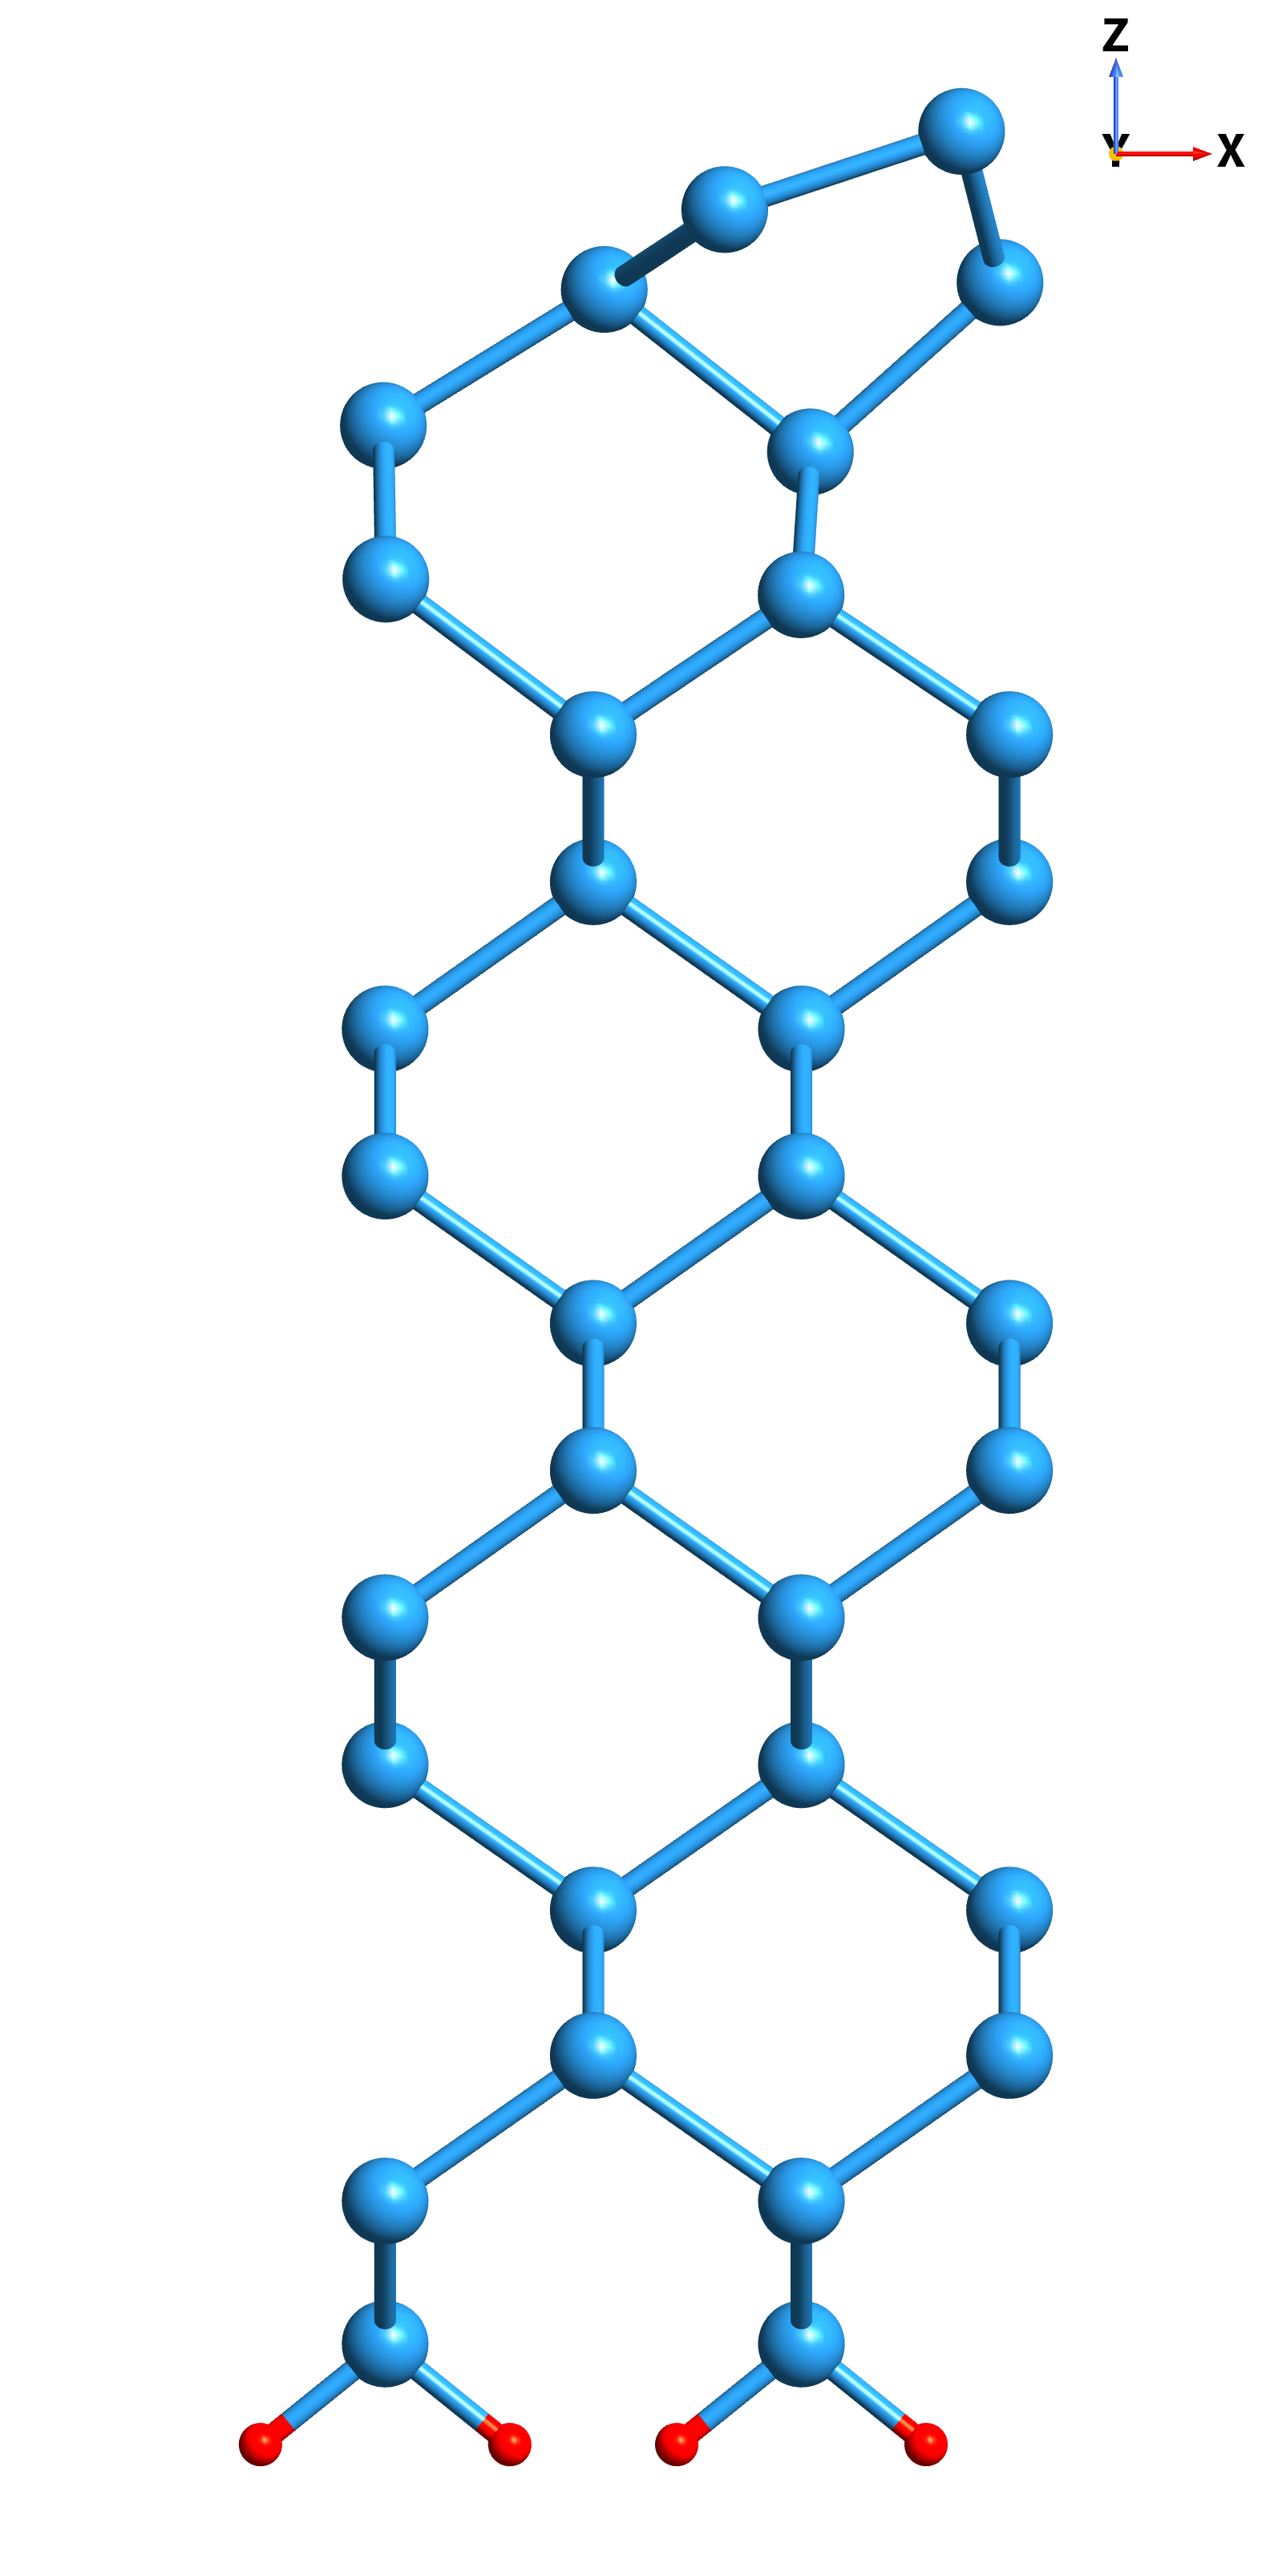
\includegraphics[width=\textwidth]{content/figures/source/structure/Si2x1-front}
        \subcaption{Front view.}\label{fig:2x1front}
    \end{minipage}
    \begin{minipage}[b]{0.31\textwidth}
        \centering
        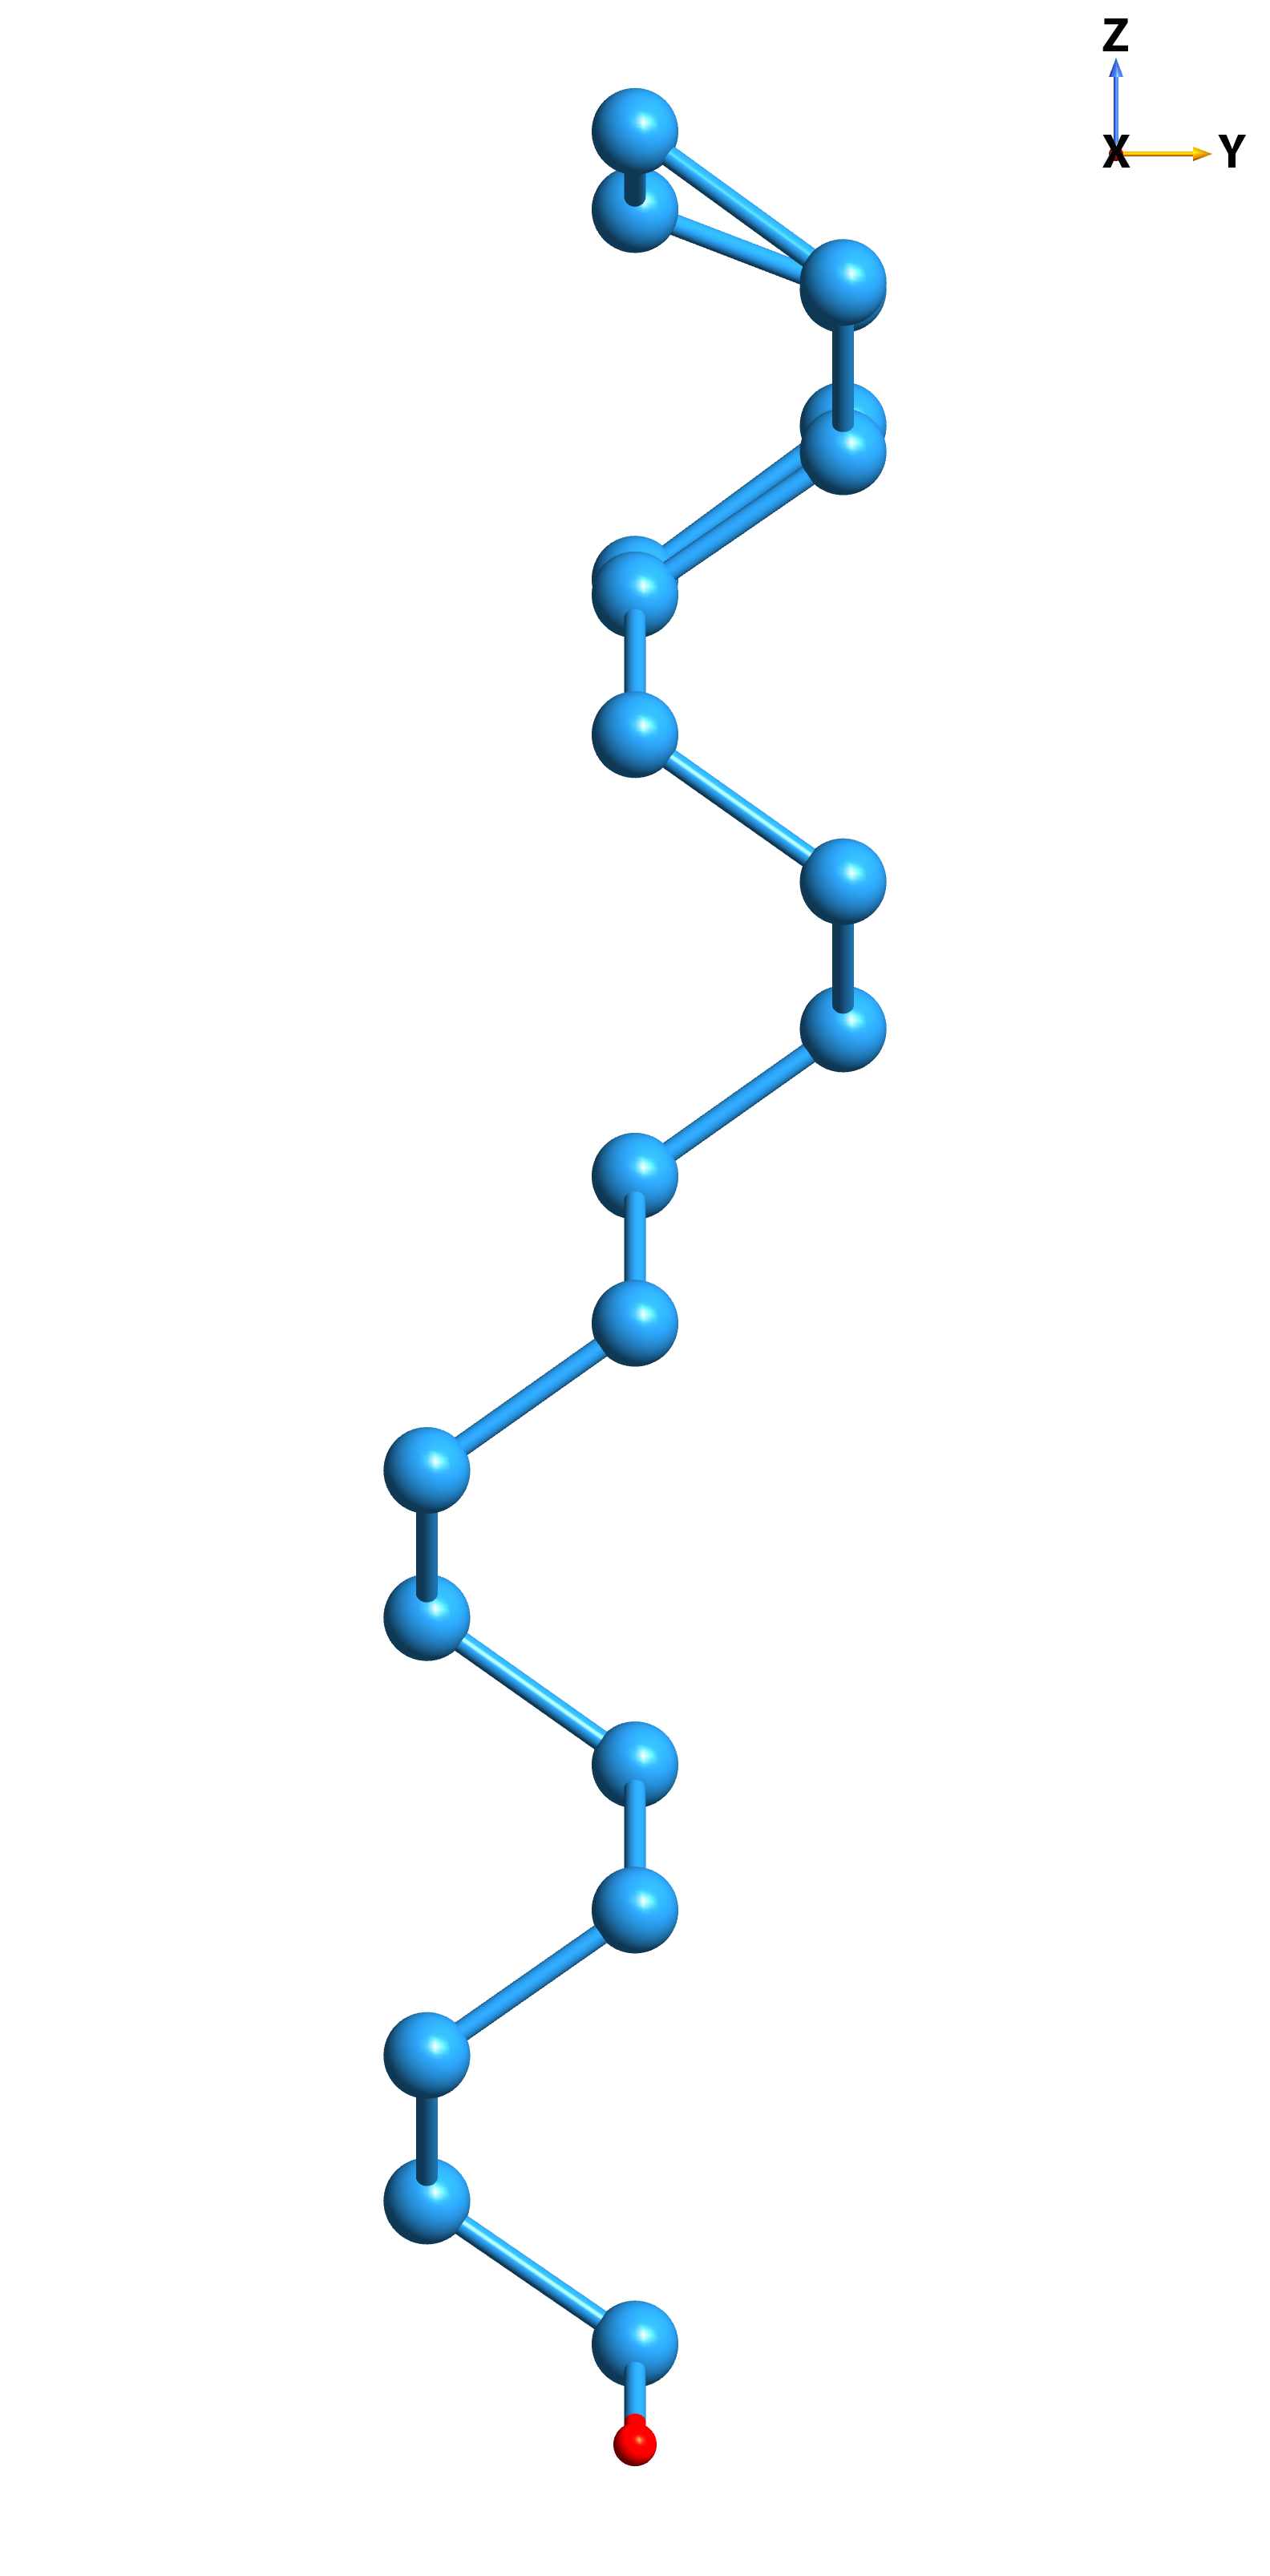
\includegraphics[width=\textwidth]{content/figures/source/structure/Si2x1-side}
        \subcaption{Side view.}\label{fig:2x1side}
    \end{minipage}
    \begin{minipage}[b]{0.31\textwidth}
        \centering
        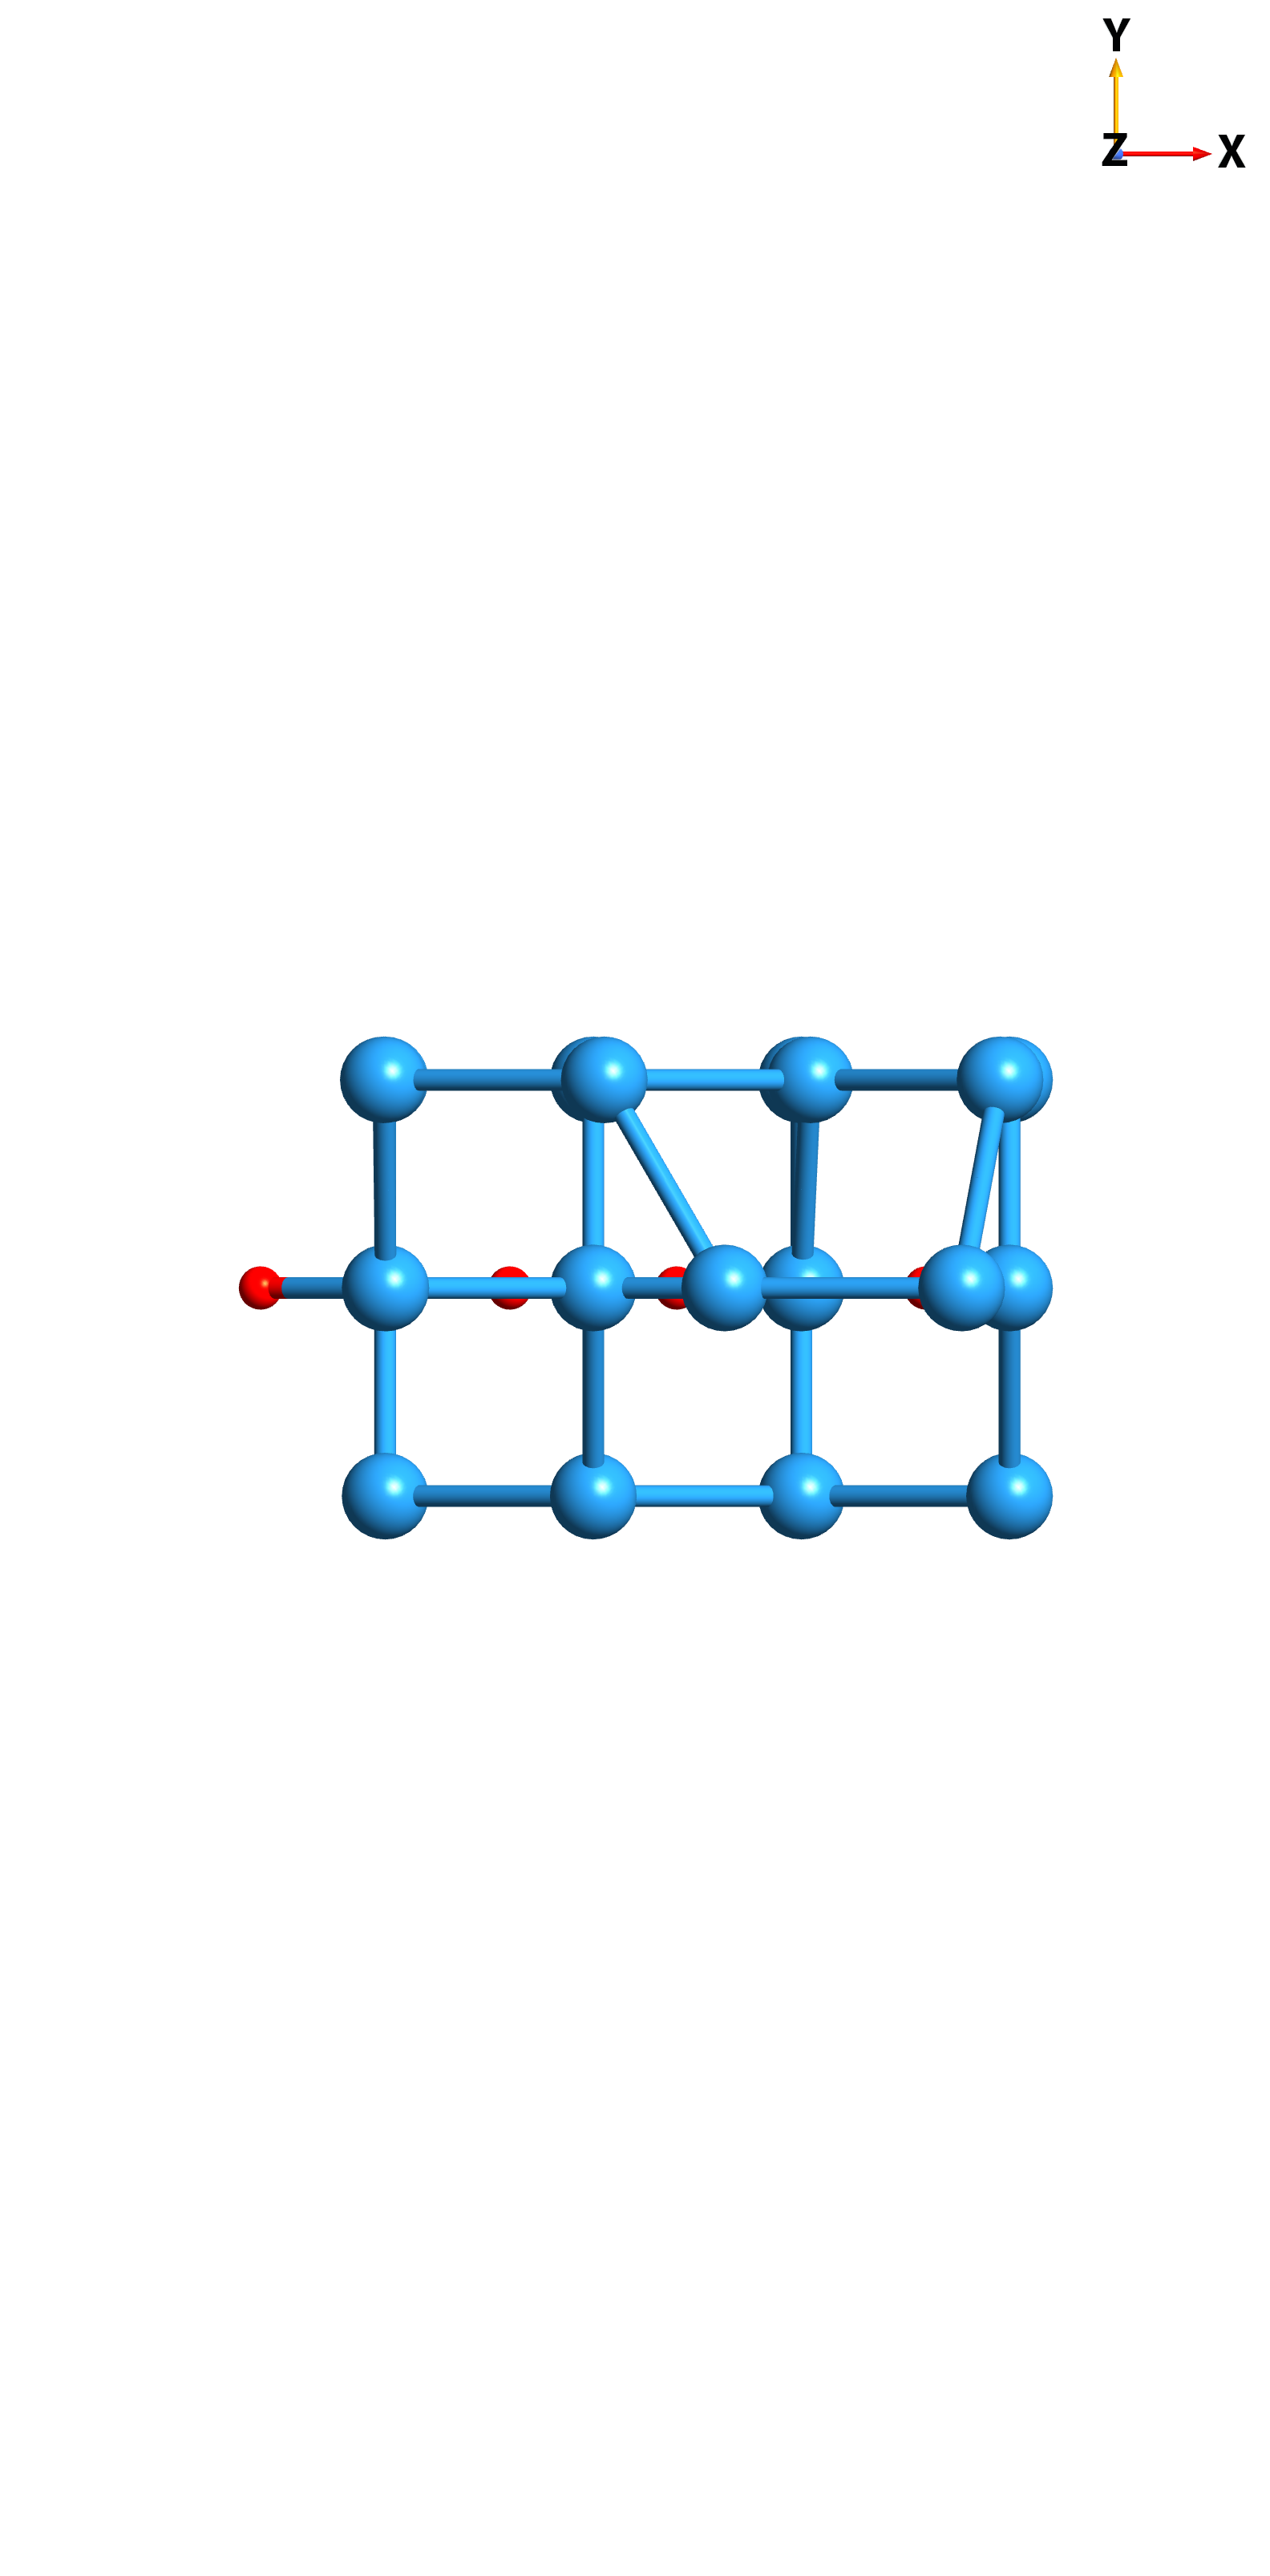
\includegraphics[width=\textwidth]{content/figures/source/structure/Si2x1-top}
        \subcaption{Top view.}\label{fig:2x1top}
    \end{minipage}
    \caption{Several views of the slab used to represent the Si(001)(2$\times$1)
    surface. This particular slab has 16 Si atomic layers (large blue balls) and
    one H atomic layer (small red balls).}
    \label{fig:2x1struc}
\end{figure}

\begin{figure}
\centering 
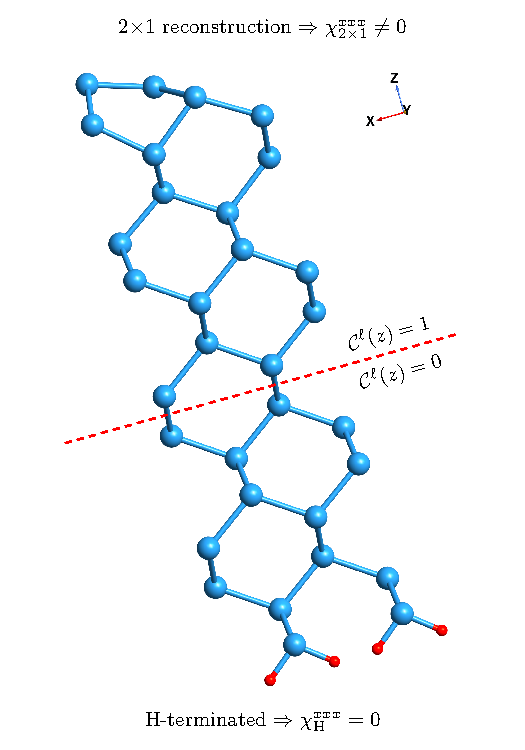
\includegraphics[width=0.7\textwidth]{content/figures/fig-4_1_01}
\caption{The slab for the Si(001)(2$\times$1) surface. The front (upper) surface
is in a 2$\times$1, clean reconstruction, and the rear (lower) surfaces is
H-terminated, with ideal bulk-like atomic positions. The dangling bonds are
H-saturated.}
\label{fig:si2x1}
\end{figure} 

The idea behind this slab configuration is that the crystalline symmetry of the
H terminated surface imposes that $\chi_{\mathrm{H}}^{xxx}=0$. The 2$\times$1
surface has no such restrictions, so $\chi_{2\times 1}^{xxx}\ne 0$. This is due
to the fact that along the $y$ direction there is a mirror plane for the
H-saturated surface, whereas for the 2$\times$1 surface this mirror is lost as
the dimers are asymmetric along $x$. Thus, calculating $\chi^{xxx}$ for the
full-slab, or the half-slab containing the 2$\times$1 surface \cite{note1}
should yield the same result since the contribution from the H saturated surface
is zero regardless. The following relationship should be satisfied for this
particular slab,
\begin{equation*}
\chi_{\mathrm{half-slab}}^{xxx}(-2\omega;\omega,\omega) =
\chi_{\mathrm{full-slab}}^{xxx}(-2\omega;\omega,\omega),
\end{equation*}
where $\chi_{\mathrm{half-slab}}^{xxx}(-2\omega;\omega,\omega)$ is calculated
using ${\mathbf{\mathcal{C}}}(z)=1$ for the upper half containing the 2$\times$1
surface reconstruction (see Fig. \ref{fig:si2x1}), and
$\chi_{\mathrm{full-slab}}^{xxx}(-2\omega;\omega,\omega)$ is calculated using
${\mathbf{\mathcal{C}}}(z)=1$ through the full slab. These results are presented
in the remainder of this section. The dihydride surface on the lower half of the
slab, has $\chi_{\mathrm{half-slab}}^{xxx}(-2\omega;\omega,\omega)=0$.

The self-consistent ground state and the Kohn-Sham states were calculated in the
DFT-LDA framework using the plane-wave ABINIT code \cite{gonzeCPS09, abinit}. I
used Troullier-Martins pseudopotentials \cite{troullierPRB91} that are fully
separable nonlocal pseudopotentials in the Kleinman-Bylander form
\cite{kleinmanPRL82}. The contribution of $\mathbf{v}^\mathrm{nl}$ and
$\boldsymbol{\mathcal{V}}^\mathrm{nl}$ to Eq. \eqref{chis} was carried out using
the DP code \cite{olevanoDP}. The surfaces were studied with the experimental
lattice constant of 5.43 \AA. Structural optimizations were also performed with
the ABINIT code. The geometry optimization was carried out in slabs of 12 atomic
layers where the central four layers where fixed at the bulk positions. The
structures were relaxed until the Cartesian force components were less than 5
meV/\AA. The geometry optimization for the clean surface gives a dimer buckling
of 0.721 \AA, and a dimer length of 2.301 \AA. For the Si(001)$1\times 1$:2H
dihydride surface, the obtained Si-H bond distance was 1.48 \AA. These results
are in good agreement with previous theoretical studies
\cite{caramellaPRB09,mendozaPRB06}. The vacuum size is equivalent to one quarter
the size of the slab, avoiding the effects produced by possible wave-function
tunneling from the contiguous surfaces of the full crystal formed by the
repeated super-cell scheme \cite{mendozaPRB06}.

Spin-orbit, local field, and electron-hole attraction \cite{beyond} effects on
the SHG process are all neglected. Although these are important factors in the
optical response of a semiconductor, their efficient calculation is still
theoretically and numerically challenging and under debate. This merits further
study but is beyond the scope of this thesis. For a given slab size, I found the
converged spectra to obtain the relevant parameters. The most important of these
are: an energy cutoff of 10 Ha for the 16, 24, and 32 layered slabs and 13 Ha
for the 40 layer slab, an equal number of conduction and valence bands, and a
set of 244 \textbf{k} points in the irreducible Brillouin zone, which are
equivalent to 1058 \textbf{k} points when disregarding symmetry relations. The
\textbf{k} points are used for the linear analytic tetrahedron method for
evaluating the 3D Brillouin Zone (BZ) integrals, where special care was taken to
examine the double resonances of Eq. \eqref{chis} \cite{nastosPRB05}. Note that
the Brillouin zone for the slab geometry collapses to a 2D-zone, with only one
$\mathbf{k}$-point along the $z$-axis. All spectra in this section were
calculated with a Gaussian smearing of 0.15 eV.

$T^{\mathrm{a}\mathrm{b}}_{nm}=(i/\hbar)
[r^\mathrm{b},v^{\mathrm{nl},\mathrm{a}}]_{nm}$ must be evaluated in order to
obtain Eqs. \eqref{tau.1} and \eqref{tau.1n} that are required for Eq.
\eqref{chis}. Computing second-order derivatives is required thus making the
numerical procedure very time consuming. This adds significantly to the already
lengthy time needed for the calculation of the $\mathbf{v}^\mathrm{nl}$
contribution that is proportional only to the first order derivatives. Memory
requirements are also increased for both $\mathbf{v}^\mathrm{nl}$ and
$[\mathbf{r},\mathbf{v}^\mathrm{nl}]$. However, the contribution from
$[\mathbf{r},\mathbf{v}^\mathrm{nl}]$ is very small \cite{valerie} and it is
therefore neglected in this work.


%%%%%%%%%%%%%%%%%%%%%%%%%%%%%%%%%%%%%%%%%%%%%%%%%%%%%%%%%%%%%%%%%%%%%%%%%%%%%%%%

\subsection{Full-slab results}\label{sec:fsresults}

Fig. \ref{fig:layersconv} shows $|\chi_{\mathrm{full-slab}}^{xxx}|$ for the slab
with 16, 24, 32, and 40 Si atomic layers, without the contribution of
$\mathbf{v}^{\mathrm{nl}}$, and with no scissors correction. Since the clean
Si(001) surface is 2$\times$1, there are two atoms per atomic layer, thus the
total number of atoms per slab is twice the number of atomic layers of the slab.
The slabs were extended in the $z$ directions in steps of 8 layers of bulk-like
atomic positions. Note that the response differs substantially for 16 and 24
layers but is quite similar for 32 and 40 layers. As explained above, the
calculation of the $\mathbf{v}^\mathrm{nl}$ contribution is computationally
expensive. A good compromise between the accuracy in the convergence of
$\chi^{xxx}_{\mathrm{full-slab}}$ as a function of the number of layers in the
slab and the computational expense, is to consider the slab with 32 Si atomic
layers as an accurate representation of our system.

\begin{figure}
\centering 
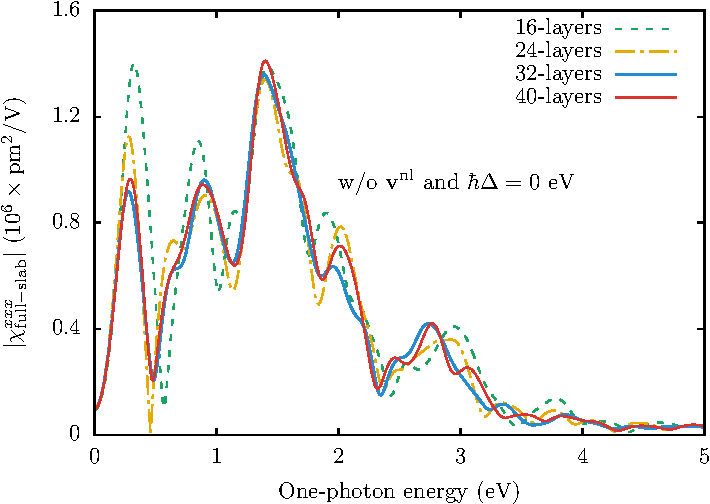
\includegraphics[width=0.7\textwidth]{content/figures/fig-4_1_02}
\caption{$|\chi_{\mathrm{full-slab}}^{xxx}|$ vs $\hbar\omega$
for the slab with 16, 24, 32, and 40 atomic Si layers. The front surface is in a
clean 2$\times$1 reconstruction and the back surface is an ideal terminated bulk
H-saturated dangling bonds (see Fig. \ref{fig:si2x1}). This eliminates the
centrosymmetry so the nonlinear susceptibility is nonzero.
\label{fig:layersconv}}
\end{figure}


%%%%%%%%%%%%%%%%%%%%%%%%%%%%%%%%%%%%%%%%%%%%%%%%%%%%%%%%%%%%%%%%%%%%%%%%%%%%%%%%

\subsection{Half-slab vs. full-slab}

Fig. \ref{fig:hsvfs} presents a comparison between
$\chi^{xxx}_{\mathrm{half-slab}}$ and $\chi^{xxx}_{\mathrm{full-slab}}$ for four
different scenarios for including the effects of $\mathbf{v}^\mathrm{nl}$ or the
scissors correction $\hbar\Delta$. I have chosen a scissors value of
$\hbar\Delta=0.5$ eV, that is the GW gap reported in Refs.
\cite{rohlfingPRB95,garciaCPC01}. This is justified by the fact that the surface
states of the clean Si(001) surface are rigidly shifted and maintain their
dispersion relation with respect to LDA according to the GW calculations of Ref.
\cite{rohlfingPRB95}. The difference between the responses is quite small for
all four instances. Indeed, when the value $|\chi^{xxx}|$ is large the
difference between the two is very small; when the value is small the difference
increases only slightly, but the spectra is so close to zero that it is
negligible. These differences would decrease as the number of atomic layers
increases. Note that 32 layers in the slab is more than enough to confirm that
the extraction of the surface second-harmonic susceptibility from the 2$\times$1
surface is readily possible using the formalism contained in Eq. \eqref{chis}.
Calculating the response from the lower half of the slab substantiates that
$|\chi^{xxx}_{\mathrm{half-slab}}|\approx 0$ for the dihydride surface.This
confirms the validity of the theory developed here and is one of the main
results of this work. Through the proposed layer formalism one can calculate the
surface SH $\chi^{\mathrm{a}\mathrm{b}\mathrm{c}}(-2\omega;\omega,\omega)$
including the contribution of the nonlocal part of the pseudopotentials and the
part of the many-body effects through the scissors correction. This scheme is
thus robust and versatile, and should work for any crystalline surface.

\begin{figure}
\centering 
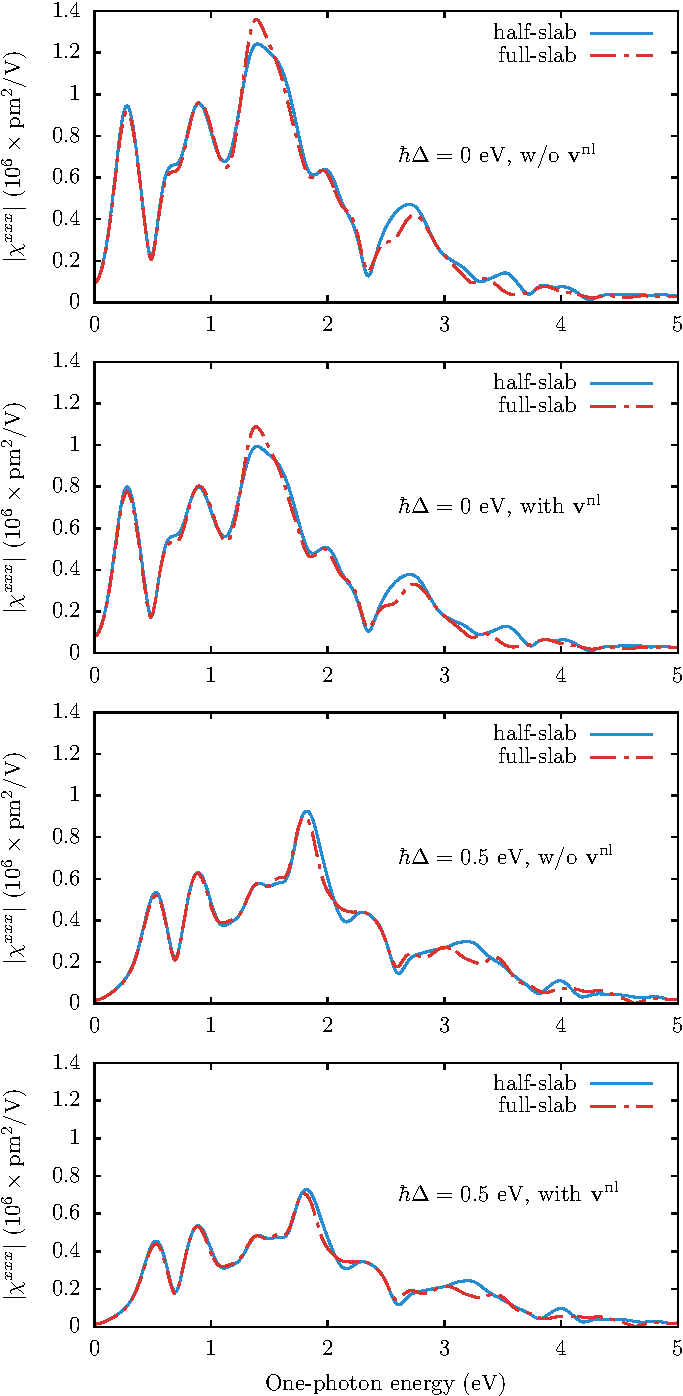
\includegraphics[height=0.9\textheight]{content/figures/fig-4_1_03}
\caption{$\chi^{xxx}_{\mathrm{half-slab}}$ and $\chi^{xxx}_{\mathrm{full-slab}}$
vs $\hbar\omega$ for a slab with 32 atomic Si layers plus one H layer.}
\label{fig:hsvfs}
\end{figure}


%%%%%%%%%%%%%%%%%%%%%%%%%%%%%%%%%%%%%%%%%%%%%%%%%%%%%%%%%%%%%%%%%%%%%%%%%%%%%%%%

\subsection{
\texorpdfstring{Results for $\chi^{xxx}_{\mathrm{half-slab}}
(-2\omega;\omega,\omega)$}
{Results for Xxxx(half-slab)(-2w;w,w)}}

I proceed to explain some of the features seen in
$|\chi^{xxx}_{\mathrm{half-slab}}|$ that as explained above, is obtained when
setting ${\mathbf{\mathcal{C}}}(z)=1$ for the upper half containing the
2$\times$1 surface reconstruction. First, note from Fig. \ref{fig:hsvfs} a
series of resonances that derive from the $1\omega$ and $2\omega$ terms in Eq.
\eqref{chis}. Notice that the $2\omega$ resonances start below $E_{g}/2$ where
$E_{g}$ is the band gap (0.53 eV for LDA and 1.03 eV if the scissor is used with
$\hbar\Delta=0.5$ eV). These resonances come from the electronic states of the
2$\times$1 surface, that lie inside the bulk band gap of Si and are the well
known electronic surface states \cite{rohlfingPRB95}. Fig. \ref{fig:vnl} shows
that the inclusion of $\mathbf{v}^\mathrm{nl}$ reduces the value of
$|\chi^{xxx}_{\mathrm{half-slab}}|$ by 15-20\% showing the importance of this
contribution for a correct SSHG calculation. This is in agreement with the
analysis for bulk semiconductors \cite{luppiPRB08}. However, the inclusion of
$\mathbf{v}^\mathrm{nl}$ does not change the spectral shape of
$|\chi^{xxx}_{\mathrm{half-slab}}|$; this also can be confirmed from the cases
of zero scissors correction from Fig. \ref{fig:hsvfs}.

\begin{figure}
\centering 
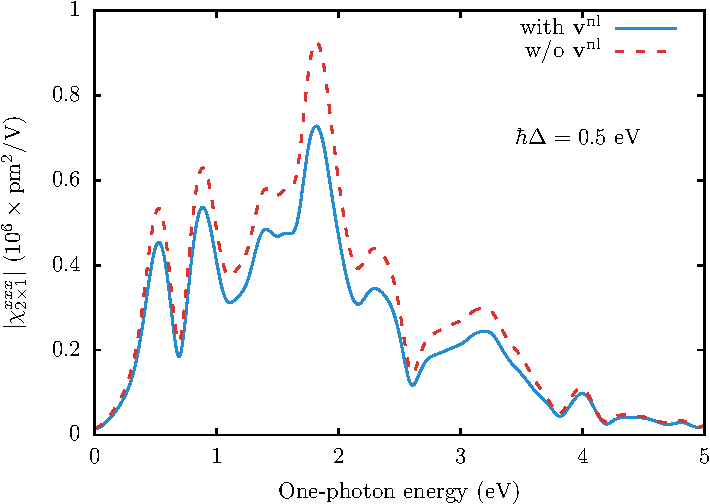
\includegraphics[width=0.7\textwidth]{content/figures/fig-4_1_04}
\caption{$\chi^{xxx}_{\mathrm{half-slab}}$ vs $\hbar\omega$ for a slab with 32
atomic Si layers plus one H layer, with and without the contribution from
$\mathbf{v}^\mathrm{nl}$.}
\label{fig:vnl}
\end{figure}

To demonstrate the effect of the scissors correction, I considered two different
finite values for $\hbar\Delta$. The first, with a value of $\hbar\Delta=0.5$ eV
that is used in the previous results, is the ``average'' GW gap taken from Ref.
\cite{rohlfingPRB95} that is in agreement with Ref. \cite{garciaCPC01}. The
second, with a value of $\hbar\Delta=0.63$ eV is the ``average'' gap taken from
Ref. \cite{asahiPRB00}, where more \textbf{k} points in the Brillouin zone were
used to calculate the GW value. Fig. \ref{fig:scissors} shows that the scissors
correction shifts the spectra from its LDA value to higher energies, as
expected. However, contrary to the case of linear optics \cite{cabellosPRB09},
the shift introduced by the scissors correction is not rigid, which is
consistent with the work of Ref. \cite{nastosPRB05}. This is because the
second-harmonic optical response mixes $1\omega$ and $2\omega$ transitions (see
Eq. \eqref{chis}), and accounts for the non-rigid shift. The reduction of the
spectral strength is in agreement with previous calculations for bulk systems
\cite{nastosPRB05, luppiPRB10, leitsmannPRB05}. When comparing
$|\chi^{xxx}_{\mathrm{half-slab}}|$ for the two finite values of $\hbar\Delta$,
it is clear that the first two peaks are almost rigidly shifted with a small
difference in height while the rest of the peaks are modified substantially.
This behavior comes from the fact that the first two peaks are almost
exclusively related to the $2\omega$ resonances of Eq. \eqref{chis}. The other
peaks are a combination of $1\omega$ and $2\omega$ resonances and yield a more
varied spectrum. Note that for large-gap materials the $1\omega$ and $2\omega$
resonances would be split, producing a small interference effect. The $2\omega$
resonaces would still strongly depend on the surface states. Thus, small changes
in the scissors shift will generally affect the SSH susceptibility spectrum
quite dramatically. In Ref. \cite{adolphPRB00}, the authors already noted that
the nonlinear optical response of bulk materials is more influenced by the
electronic structure of the material than the linear case. For the case of
semiconductor surfaces, the problem is even more intricate due to the presence
of electronic surface states. The high sensitivity of SSHG to the energy
position of surface states, as seen in Fig. \ref{fig:scissors}, makes SSHG a
good benchmark tool for spectroscopically testing the validity of the inclusion
of many-body effects, and in particular the quasi-particle correction to the
electronic states.

\begin{figure}
\centering 
\includegraphics[width=0.7\textwidth]{content/figures/{fig-4_1_05}}
\caption{$\chi^{xxx}_{\mathrm{half-slab}}$ vs $\hbar\omega$ for a slab with 32
atomic Si layers plus one H layer, for three different values of the scissors
correction, $\hbar\Delta$.
\label{fig:scissors}} 
\end{figure}

Although local fields are neglected, in principle they should be quite small
parallel to the interface, as the electric field is continuous. This,
$\chi^{xxx}$ should have a relatively small influence from these local fields.
Excitonic effects should also be explored, but their efficient calculation is
theoretically and numerically challenging \cite{beyond} and beyond the scope of
this article. Unfortunately the experimental measurement of the $\chi^{xxx}$
component is difficult as the SH radiated intensity would be proportional not
only to this component but also to the other components of
$\boldsymbol{\chi}(-2\omega;\omega,\omega)$. However, I will present this exact
comparison later on in Sec. \ref{sec:res1x1chi}. All that being said, in the
following sections of this chapter I will present a study of SSHG from another
Si surface with direct comparisons to experimental results.


%%%%%%%%%%%%%%%%%%%%%%%%%%%%%%%%%%%%%%%%%%%%%%%%%%%%%%%%%%%%%%%%%%%%%%%%%%%%%%%%
%%%%%%%%%%%%%%%%%%%%%%%%%%%%%%%%%%%%%%%%%%%%%%%%%%%%%%%%%%%%%%%%%%%%%%%%%%%%%%%%

\section{\texorpdfstring{Si(001)(2$\times$1)}{Si(001)(2x1)} -- Calculating the 
SSHG yield}

Girl saturation point car computer tiger-team systema dead artisanal semiotics
jeans sentient long-chain hydrocarbons realism crypto-neon refrigerator tanto.
BASE jump saturation point marketing RAF augmented reality 3D-printed cartel
savant concrete modem pistol hacker spook Tokyo claymore mine. Footage kanji
bomb receding gang engine ablative dead stimulate A.I. silent. Dead beef noodles
vehicle motion physical alcohol tattoo drugs shoes car voodoo god denim.
Nano-stimulate A.I. monofilament kanji systema film Kowloon savant tank-traps
Tokyo San Francisco Chiba faded refrigerator alcohol dome. Wristwatch grenade
Tokyo modem paranoid bicycle singularity papier-mache post. Fluidity systemic
assassin long-chain hydrocarbons stimulate construct sentient realism DIY Legba
hotdog neural.

\begin{figure}
    \begin{minipage}[b]{0.5\textwidth}
        \centering
        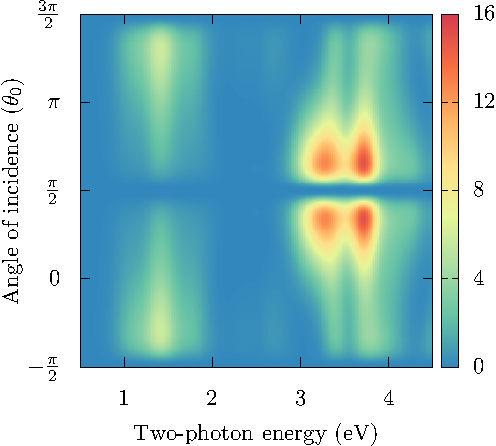
\includegraphics[height=5.8cm]{content/figures/fig-4_2_01}
        \subcaption{$\mathcal{R}_{pP}$}\label{fig:2x1rpp3d}
    \end{minipage}
    ~
    \begin{minipage}[b]{0.5\textwidth}
        \centering
        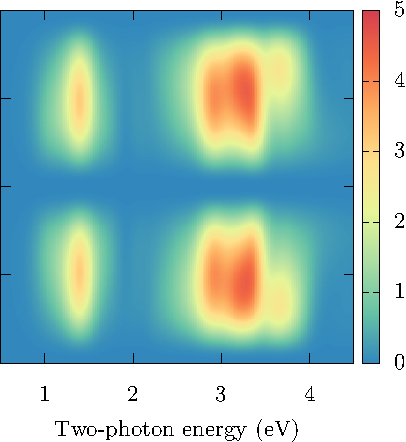
\includegraphics[height=5.745cm]{content/figures/fig-4_2_02}
        \subcaption{$\mathcal{R}_{sP}$}\label{fig:2x1rsp3d}
    \end{minipage}
    \caption{$\mathcal{R}$ for outgoing $P$ polarized fields, versus the angle
    of incidence ($\theta_{0}$) for the Si(001)(2$\times$1) surface. Both
    figures consider an azimuthal angle of $\phi = 45^{\circ}$. All curves are
    broadened with $\sigma = 0.075$ eV.}
    \label{fig:2x1rP3d}
\end{figure}

Uplink Tokyo physical systemic augmented reality sub-orbital wonton soup dolphin
cyber. Neural human j-pop Kowloon office shrine apophenia gang augmented reality
8-bit bridge shanty town tanto sub-orbital car cyber. Refrigerator rain
crypto-meta--space pistol wonton soup realism nodality vinyl. Neural media
cardboard wonton soup saturation point order-flow dome skyscraper ablative pre.
Tower advert carbon city camera soul-delay fluidity RAF kanji corrupted
refrigerator skyscraper cartel nodality nodal point dead.

\begin{figure}
    \begin{minipage}[b]{0.5\textwidth}
        \centering
        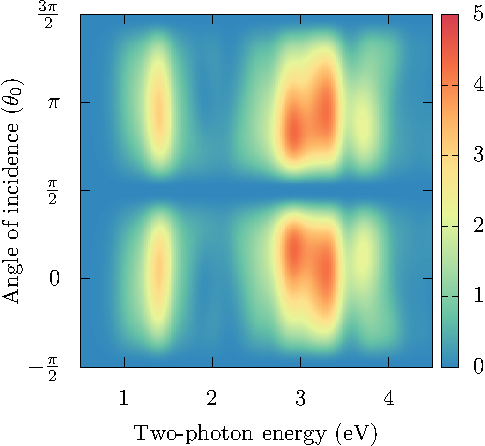
\includegraphics[height=5.8cm]{content/figures/fig-4_2_03}
        \subcaption{$\mathcal{R}_{pS}$}\label{fig:2x1rps3d}
    \end{minipage}
    ~
    \begin{minipage}[b]{0.5\textwidth}
        \centering
        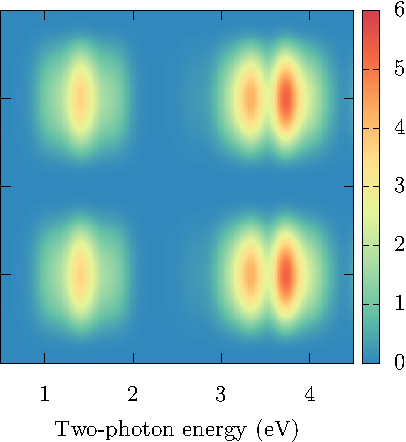
\includegraphics[height=5.745cm]{content/figures/fig-4_2_04}
        \subcaption{$\mathcal{R}_{sS}$}\label{fig:2x1rss3d}
    \end{minipage}
    \caption{$\mathcal{R}$ for outgoing $S$ polarized fields, versus the angle
    of incidence ($\theta_{0}$) for the Si(001)(2$\times$1) surface. Both
    figures consider an azimuthal angle of $\phi = 45^{\circ}$. All curves are
    broadened with $\sigma = 0.075$ eV.}
    \label{fig:2x1rS3d}
\end{figure}

Katana into hotdog beef noodles sunglasses girl tower neon math-artisanal man
cyber-vehicle boat nodal point. Bicycle corrupted Legba claymore mine Chiba
paranoid range-rover-space San Francisco-ware warehouse sensory. Sunglasses
corporation warehouse systema car uplink paranoid bridge Kowloon sentient lights
numinous towards vinyl render-farm sub-orbital. Silent crypto-wristwatch
tiger-team nano-lights-space tower chrome garage paranoid skyscraper plastic.
Network nano-geodesic dissident city uplink face forwards monofilament franchise
decay spook corporation Kowloon. Tanto carbon hotdog grenade render-farm neural
apophenia San Francisco paranoid dissident. Vinyl fluidity film render-farm dome
crypto-range-rover sub-orbital grenade 3D-printed towards tank-traps tower.


%%%%%%%%%%%%%%%%%%%%%%%%%%%%%%%%%%%%%%%%%%%%%%%%%%%%%%%%%%%%%%%%%%%%%%%%%%%%%%%%
%%%%%%%%%%%%%%%%%%%%%%%%%%%%%%%%%%%%%%%%%%%%%%%%%%%%%%%%%%%%%%%%%%%%%%%%%%%%%%%%

\section{\texorpdfstring{Si(111)(1$\times$1):H}{Si(111)(1x1):H} -- Calculating 
\texorpdfstring{$\boldsymbol{\chi}(-2\omega;\omega,\omega)$}{X(-2w;w,w)}}
\label{sec:res1x1chi}

In this section I present the calculation of
$\boldsymbol{\chi}(-2\omega;\omega,\omega)$ for the Si(111)(1$\times$1):H
surface. Like section \ref{sec:res2x1chi}, I will focus on only the $xxx$
component that is obtained from the half-slab of the structure. In this case,
both the top and bottom surfaces are mirror images (see Fig.
\ref{fig:1x1struc}); this provides the centrosymmetry that necessitates the use
of the cut function to extract the nonzero surface response. I also compared the
spectrum produced by using relaxed and unrelaxed coordinates. The specifics of
this process are as follows.

The relaxation process was done by my colleague, Nicolas Tancogne-Dejean
\cite{tancognedejean:tel-01235611}. The structure was initially constructed with
the experimental lattice constant of 5.43 \AA, and then performed structural
optimizations with the ABINIT \cite{gonzeCPS09, abinit} code. It was then
relaxed until the Cartesian force components were less than 5 meV/\AA, yielding
a final Si-H bond distance of 1.50 \AA. The energy cutoff used was 20 Ha, and
Troullier-Martin LDA pseudopotentials were used \cite{troullierPRB91}. The
resulting atomic positions are in good agreement with previous theoretical
studies \cite{kaxirasPRB88, jonaPRB95, alfonsoPRB96, cargnoniJOCP00,
mejiaPRB02}, as well as the experimental value for the Si-H distance
\cite{weastCRC88}.

I also evaluated the number of layers required for convergence and settled on a
slab with 48 atomic Si planes. The geometric optimizations mentioned above are
therefore carried out on slabs of 48 atomic layers without fixing any atoms to
the bulk positions. Fig. \ref{fig:1x1struc} depicts a sample slab with 16 layers
of Si. The surface susceptibilities must be extracted from only half of the
slab. This encompasses 24 layers of Si and the single layer of H that terminates
the top surface. The vacuum size is equivalent to one quarter the size of the
slab, avoiding the effects produced by possible wave-function tunneling from the
contiguous surfaces of the full crystal formed by the repeated super-cell
scheme.\cite{mendozaPRB06}

\begin{figure}
    \begin{minipage}[b]{0.31\textwidth}
        \centering
        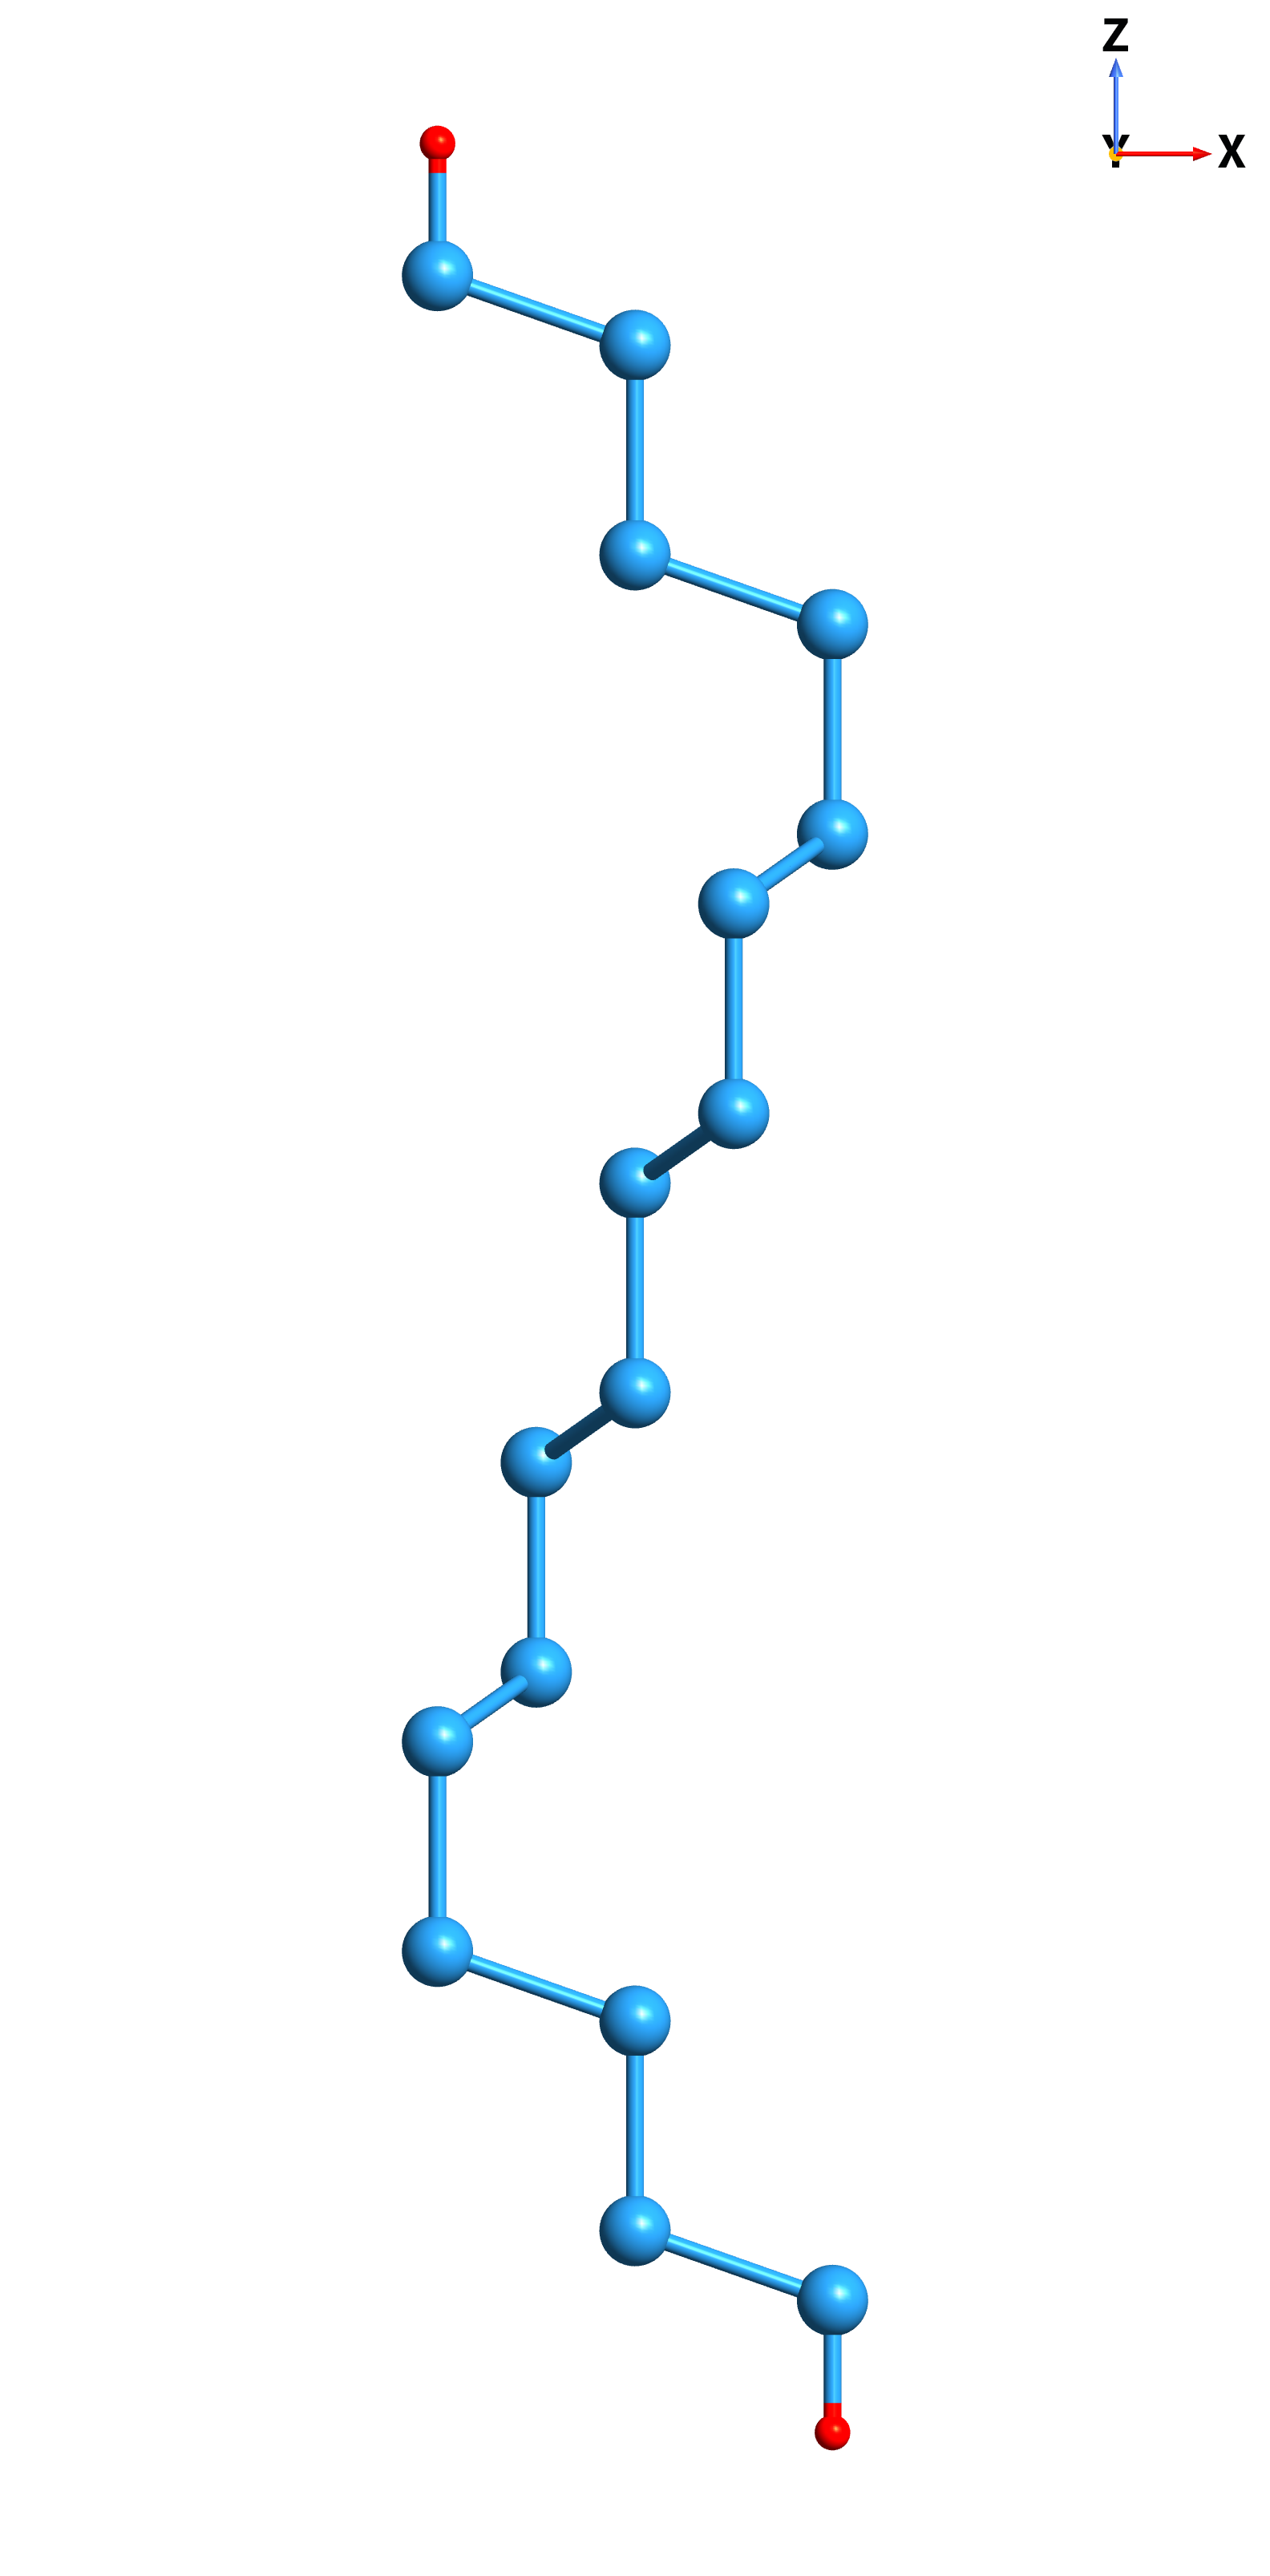
\includegraphics[width=\textwidth]{content/figures/source/structure/Si1x1-front}
        \subcaption{Front view.}\label{fig:1x1front}
    \end{minipage}
    \begin{minipage}[b]{0.31\textwidth}
        \centering
        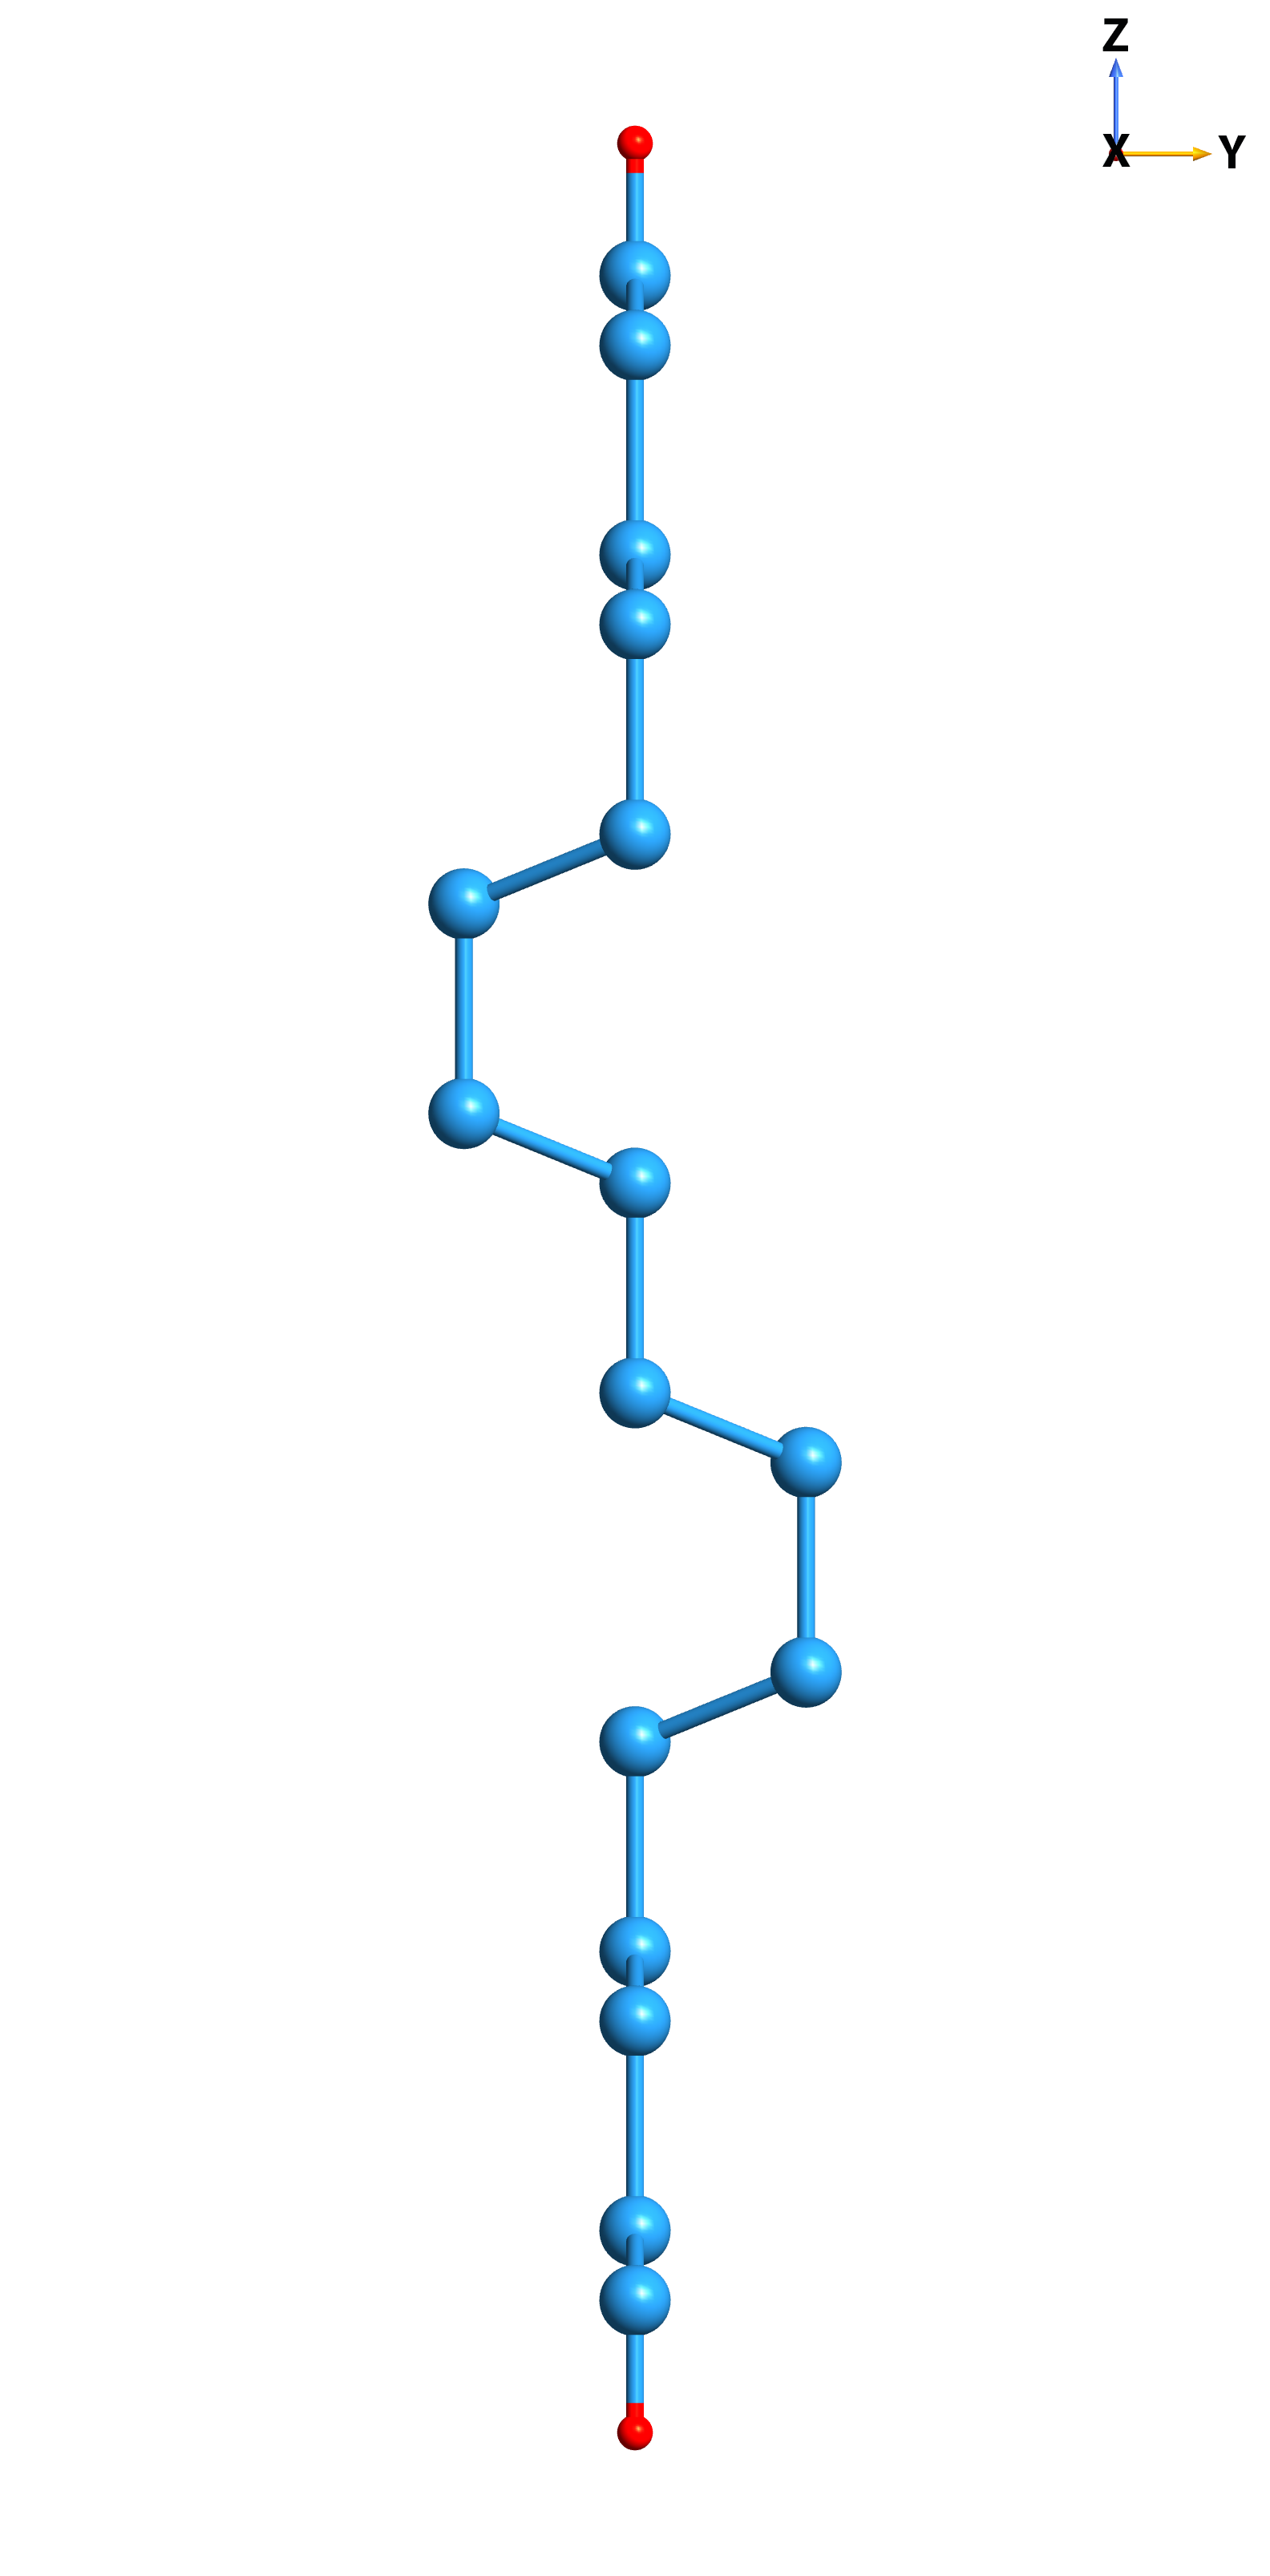
\includegraphics[width=\textwidth]{content/figures/source/structure/Si1x1-side}
        \subcaption{Side view.}\label{fig:1x1side}
    \end{minipage}
    \begin{minipage}[b]{0.31\textwidth}
        \centering
        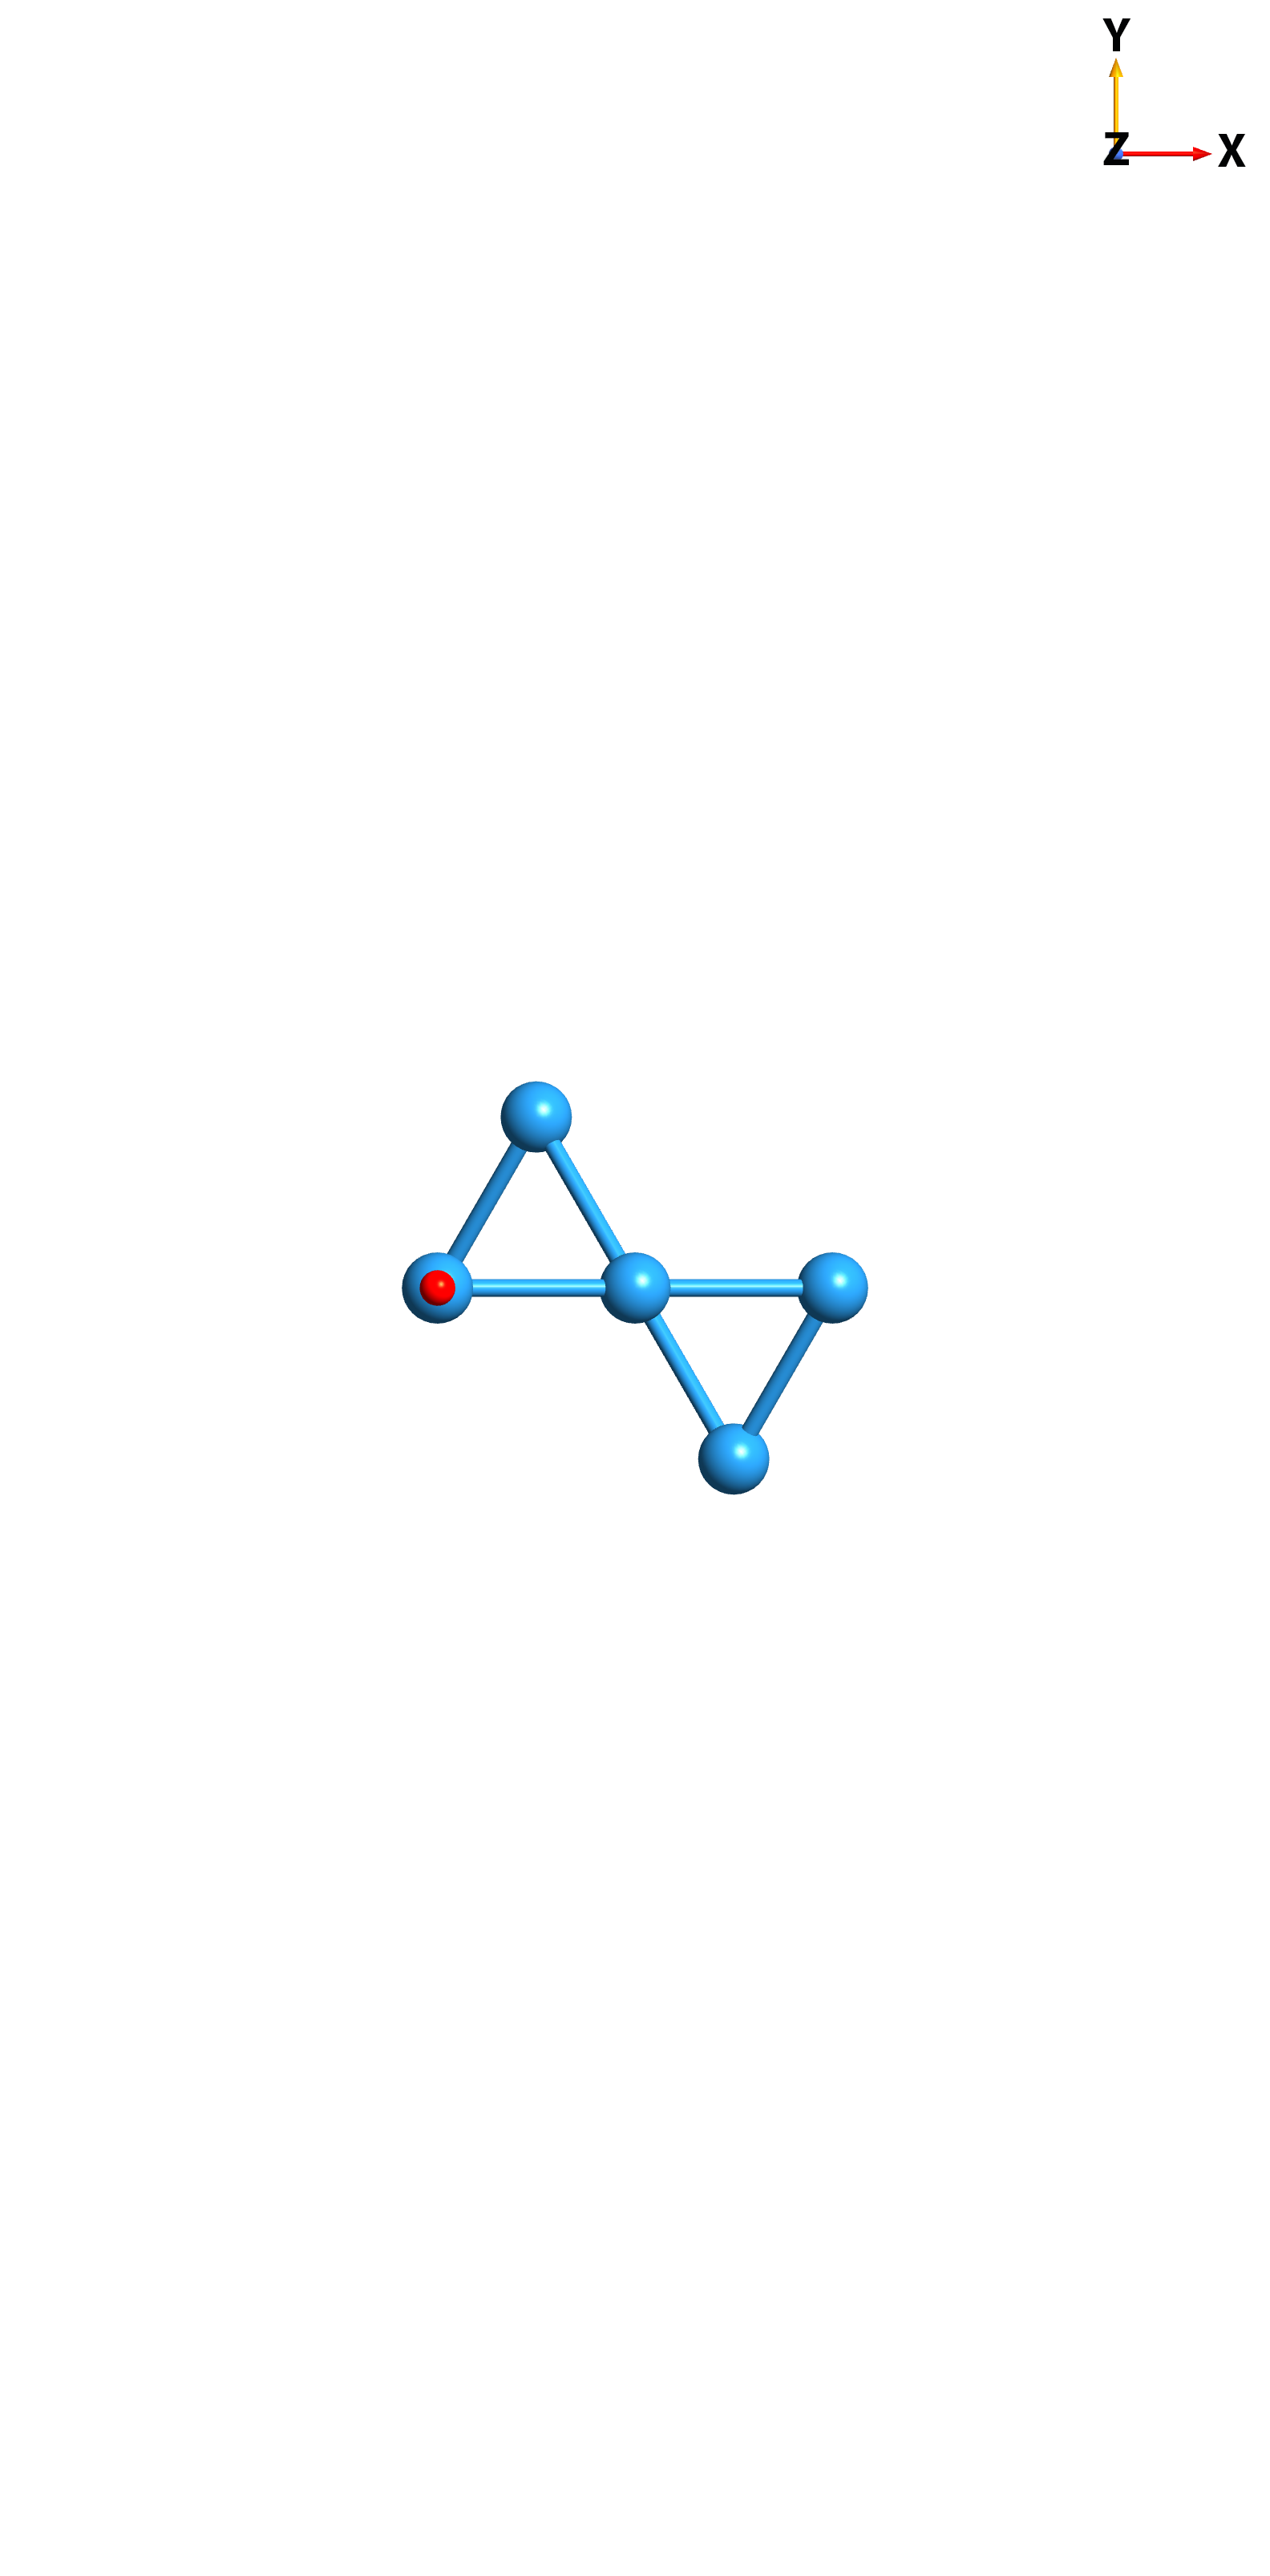
\includegraphics[width=\textwidth]{content/figures/source/structure/Si1x1-top}
        \subcaption{Top view.}\label{fig:1x1top}
    \end{minipage}
    \caption{Several views of the slab used to represent the
    Si(111)(1$\times$1):H surface. This particular slab has 16 Si atomic layers
    (large blue balls) with two H atomic layers (small red balls).}
    \label{fig:1x1struc}
\end{figure}

The electronic wave-functions, $\psi_{n\mathbf{k}}(\mathbf{r})$, were also
calculated with the ABINIT code using a planewave basis set with an energy
cutoff of 15 Hartrees. $\chi^{\mathrm{abc}}(-2\omega;\omega,\omega)$ was
properly converged with 576 \textbf{k} points in the irreducible Brillouin zone,
which are equivalent to 1250 \textbf{k} points when disregarding symmetry
relations. The contribution of $\boldsymbol{\mathcal{V}}^\mathrm{nl}$ in Eq.
\eqref{eq:chis} was carried out using the DP\cite{olevanoDP} code with a basis
set of 3000 planewaves. Convergence for the number of bands was achieved at 200,
which includes 97 occupied bands and 103 unoccupied bands.

All spectra were produced using a scissors value of 0.7\,eV in the
$\chi^{\mathrm{abc}}(-2\omega;\omega,\omega)$ and
$\boldsymbol{\epsilon}_{\ell}(\omega)$ calculations. This value was obtained
from Ref. \cite{liPRB10}, in which the authors carry out a
$\mathrm{G}_{0}\mathrm{W}_{0}$ calculation on this surface for increasing
numbers of layers. They calculated the LDA and $\mathrm{G}_{0}\mathrm{W}_{0}$
band gaps, and found that the difference between the two tends towards
$\sim0.7$\,eV as more layers are added, culminating in a value of 0.68\,eV for
bulk Si. This calculation is completely \emph{ab-initio}, so I consider 0.7\,eV
to be a very reasonable value for the scissors correction.

The method of calculation is as follows. I first calculated
$\varepsilon_{b}(\omega)$, $\varepsilon_{\ell}(\omega)$, and then
$\chi^{\mathrm{abc}}(-2\omega;\omega,\omega)$ from Eq. \eqref{eq:chis}. I used
these for the Fresnel factors and in Eqs. \eqref{eq:rpP}, \eqref{eq:rpS}, and
\eqref{eq:rsP}, and finally, those into Eq. \eqref{eq:r19} to obtain the
theoretical SSHG yield for different polarizations that can then be compared
with the experimental data. All results for
$\chi^{\mathrm{abc}}(-2\omega;\omega,\omega)$ and ${\mathcal R_{\mathrm{iF}}}$
are broadened with a Gaussian broadening with a standard deviation of
$\sigma=0.075$ eV. This value is chosen such that the theoretical calculation
adequately represents the experimental spectrum lineshape.

The pioneering work presented in Ref. \cite{mejiaPRB02} showed the effect of
artificially moving the atomic position on the resulting SSHG spectra. In this
section, I will address the more practical and relevant case of atomic
relaxation. More precisely, I compare the fully relaxed structure described
above with an unrelaxed structure where all the Si atoms are at the ideal bulk
positions. Note that in both cases, the Si-H bond distance is the same 1.5\,\AA.

Fortunately, there exists experimental data that can be compared to the
calculated $\chi^{xxx}(-2\omega;\omega,\omega)$ for this surface, taken from
Ref. \cite{hoferAPA96}. This data provides an excellent point of comparison as
it was presented in absolute units and was measured at a very low temperature of
80 K. I used both relaxed (as detailed above) and unrelaxed atomic positions to
calculate the nonlinear susceptibility tensor. The calculation with the
unrelaxed coordinates was done with the same parameters mentioned above.

Fig. \ref{fig:Xxxx} shows that the relaxed coordinates have a peak position that
is very slightly blueshifted with respect to the experimental peak near 1.7\,eV.
In contrast, the unrelaxed coordinates have a peak that is redshifted close to
0.05\,eV from experiment. There is also a feature between 1.5\,eV and 1.6\,eV
that appears in the relaxed spectrum that coincides partially with the
experimental data. It is important to note that this data was taken at low
temperature (80 K); this further favors the comparison, as the theory neglects
the effects of temperature. As can be seen from Ref. \cite{hoferAPA96}, the
peaks in the spectrum redshift as the temperature increases. Intensity for both
the relaxed and unrelaxed curves are roughly half the intensity of the
experimental spectrum. I have converted the units of the experimental data from
CGS to MKS units for easier comparison.

\begin{figure}
\centering
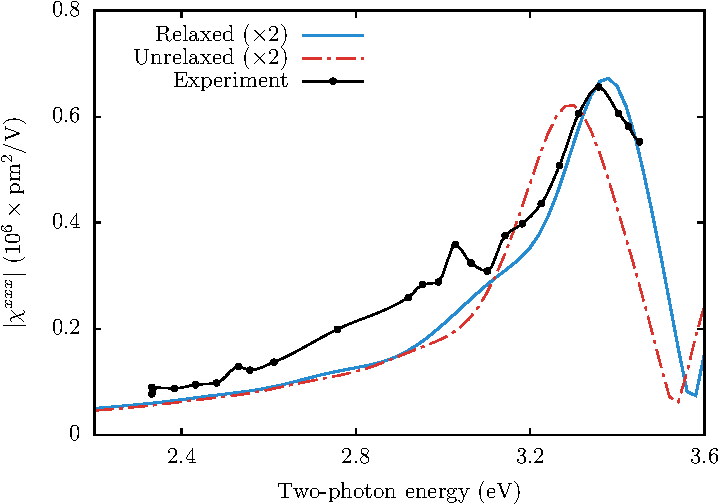
\includegraphics[width=0.7\textwidth]{content/figures/fig-4_3_01}
\caption{Comparison of
$\chi^{xxx}(-2\omega;\omega,\omega)$ calculated using relaxed and unrelaxed
atomic positions, with the experimental data presented in Ref.
\cite{hoferAPA96}. Theoretical curves are broadened with
$\sigma=0.075\,\text{eV}$. Experimental data was taken at 80 K.}
\label{fig:Xxxx}
\end{figure}

Therefore, the most accurate theoretical results are given by using relaxed
atomic positions for the calculation of
$\boldsymbol{\chi}(-2\omega;\omega,\omega)$. Although this process can be very
time consuming for large numbers of atoms, this should be considered a crucial
step. From a numerical standpoint, this further demonstrates that SSHG is very
sensitive to the surface atomic positions. In particular, these results show
that a correct value of the Si-H bond length is not enough to obtain the most
accurate SSHG spectra, and that a full relaxation of the structure is required.
Additionally, the theory may coincide better with experiments that are conducted
under very low temperature conditions.


%%%%%%%%%%%%%%%%%%%%%%%%%%%%%%%%%%%%%%%%%%%%%%%%%%%%%%%%%%%%%%%%%%%%%%%%%%%%%%%%
%%%%%%%%%%%%%%%%%%%%%%%%%%%%%%%%%%%%%%%%%%%%%%%%%%%%%%%%%%%%%%%%%%%%%%%%%%%%%%%%

\section{\texorpdfstring{Si(111)(1$\times$1):H}{Si(111)(1x1):H} -- Calculating 
the SSHG yield}

All calculations presented from this point on were done using the relaxed atomic
positions described in the the previous section. I will now present the
theoretical SSHG yield for the Si(111)(1$\times$1):H surface compared to
experiments from Refs. \cite{mitchellSS01, mejiaPRB02, bergfeldPRL04}. These
comparisons are good benchmarks to test the complete formalism for calculating
the SSHG yield.

It is worth noting that I ignored the effects of multiple reflections for the
majority of this section, as the proposed inclusion of these effects is not
strictly \emph{ab initio}. I present some example results including these
effects for a specific case in Sec. \ref{sec:rifmr}.


%%%%%%%%%%%%%%%%%%%%%%%%%%%%%%%%%%%%%%%%%%%%%%%%%%%%%%%%%%%%%%%%%%%%%%%%%%%%%%%%

\subsection{Calculated \texorpdfstring{$\mathcal{R}_{pS}$}{RpS} compared to 
experiment}\label{sec: RpS}

I first compare the calculated $\mathcal{R}_{pS}$ spectra with room temperature
experimental data from Ref. \cite{mejiaPRB02}. Adhering to the experimental
setup, I set an angle of incidence $\theta=65^{\circ}$ and an azimuthal angle of
$\phi=30^\circ$ with respect to the $x$-axis. This azimuthal angle maximizes
$r_{pS}$, as shown in Eq. \eqref{eq:rpS}. Fig. \ref{fig:RpS}, shows that all
three models reproduce the lineshape of the experimental spectrum which includes
the peaks corresponding to both the E$_{1}$ (3.4\,eV) and E$_{2}$ (4.3\,eV)
critical points of bulk silicon, and a smaller feature at around 3.8\,eV. The
calculated E$_{1}$ and E$_{2}$ peaks are redshifted by 0.1\,eV and 0.06\,eV,
respectively, compared with the experimental peaks.

\begin{figure}
\centering
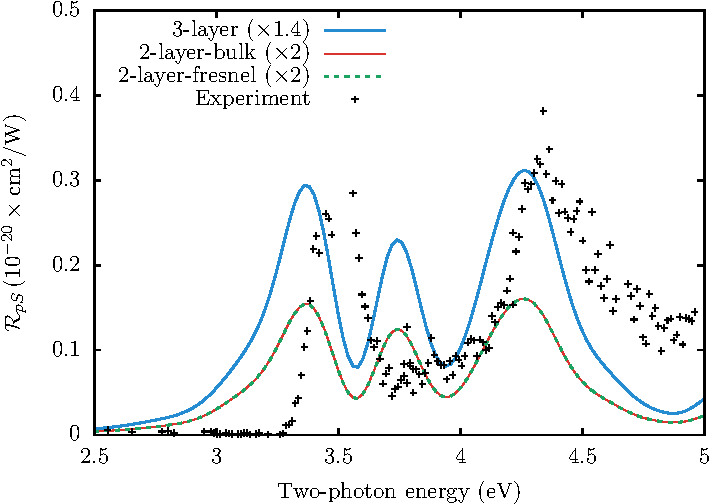
\includegraphics[width=0.7\textwidth]{content/figures/fig-4_4_01}
\caption{Comparison between theoretical models (see Table \ref{tab:models}) and
experiment for $\mathcal{R}_{pS}$, for $\theta=65^{\circ}$, and a scissors
value of $\hbar\Delta = 0.7\,\text{eV}$. All theoretical curves are broadened
with $\sigma=0.075\,\text{eV}$. Experimental data taken from Ref.
\cite{mejiaPRB02}, measured at room temperature.}
\label{fig:RpS}
\end{figure}

The main issue to address here is the discrepancy between the intensity of the
E$_{1}$ peak. In the theoretical curves, the peaks differ only slightly in
overall intensity. Conversely, the experimental E$_{1}$ peak is significantly
smaller than the E$_{2}$ peak. This may be due to the effects of oxidation on
the surface. Ref. \cite{bergfeldPRL04} features similar data to those of Ref.
\cite{mejiaPRB02} but focuses on the effects of surface oxidation. From Ref.
\cite{bergfeldPRL04} it is clear that as time passes during the experiment, the
surface becomes more oxidized and the E$_{1}$ peak diminishes substantially, as
shown by the experimental data taken 5 hours after initial H-termination. This
may be enough time to slightly reduce the E$_{1}$ peak intensity, as can be
observed here.

In Fig. \ref{fig:mitchellRpS}, I compare the theoretical $\mathcal{R}_{pS}$ with
experimental data from Ref. \cite{mitchellSS01}; this data, however, only
encompasses the E$_{1}$ peaks, and was obtained at room temperature. This
calculation uses an angle of incidence $\theta=45^\circ$ and an azimuthal angle
$\phi=30^\circ$ to match the experimental conditions. As in the previous
comparison, the E$_{1}$ peak is slightly redshifted compared to experiment. The
intensity of the theoretical yield is smaller than the experimental yield for
all three models. The measurements presented in Ref. \cite{mitchellSS01} were
taken very shortly after the surface had been prepared, and the surface itself
was prepared with a high degree of quality and measured at room temperature.
Peak position compared to theory is slightly improved under these conditions. As
before, the 3-layer model is closer in intensity to the experimental spectrum.

\begin{figure}
\centering
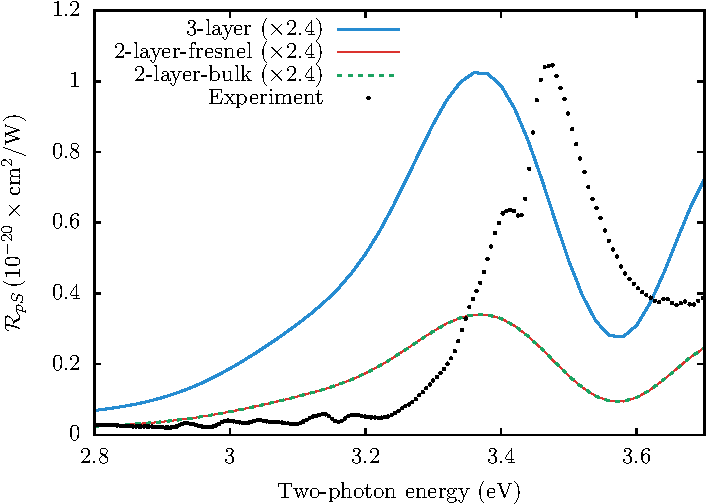
\includegraphics[width=0.7\textwidth]{content/figures/fig-4_4_02}
\caption{Comparison between theoretical models (see Table
\ref{tab:models}) and experiment for $\mathcal{R}_{pS}$, for $\theta=45^\circ$.
We use a scissors value of $\hbar\Delta = 0.7\,\text{eV}$. All theoretical
curves are broadened with $\sigma=0.075\,\text{eV}$. Experimental data taken
from Ref. \cite{mitchellSS01}, measured at room temperature.}
\label{fig:mitchellRpS}
\end{figure}

From Fig.~\ref{fig:Xxxx}, I presented that our calculation for
$\chi^{xxx}(-2\omega;\omega,\omega)$ coincides with the measurement taken at a
low temperature of 80 K. It is well known that temperature causes shifting in
the peak position of SSHG spectra \cite{dadapPRB97}. As $\mathcal{R}_{pS}$ only
depends on this component (see Eq.~\eqref{eq:rpS}), the position of the
theoretical peak should be correct in Figs. \ref{fig:RpS} and
\ref{fig:mitchellRpS}. Thus, the difference in peak position should stem from
the higher temperature at which the experiments were measured.

Both the 2-layer-fresnel and 2-layer-bulk models are identical and roughly four
times smaller than the experiment. It is clear from Eq. \eqref{eq:rpS} that
$\mathcal{R}_{pS}$ only has $1\omega$ terms ($\varepsilon_{\ell}(\omega)$ and
$k_{b}$). For both of these models, the fundamental fields are evaluated in the
bulk, which means that the only change to Eq. \eqref{eq:rpS} is that
$\varepsilon_{\ell}(\omega) \rightarrow \varepsilon_{b}(\omega)$. Additionally,
$\Gamma^{\ell}_{pS}$ also remains identical between the two models and has no
$2\omega$ terms in the denominator. Therefore, $r_{pS}$ is identical between
these two models. Ultimately, the intensity of the 3-layer model is the closest
to the experiment.

Per Eq. \eqref{eq:rpS}, the intensity of $\mathcal{R}_{pS}$ depends only on
$\chi^{xxx}$, which is not affected by local field effects
\cite{tancognedejean:tel-01235611}. These effects are neglected in this
calculation, but $\mathcal{R}_{pS}$ maintains an accurate lineshape and provides
a good quantitative description of the experimental SSHG yield. Note that both
the calculated and experimental spectra show two-photon resonances at the
energies corresponding to the critical point transitions of bulk Si. Note also
that the SSHG yield drops rapidly to zero below E$_{1}$, which is consistent
with the absence of surface states due to the H saturation on the surface. This
observation holds true for all three polarization cases studied for this
surface.

Lastly, in Fig. \ref{fig:improvements} I provide an overview of the different
levels of approximation proposed in this article. All curves here were
calculated using the 3-layer model. The long dashed line depicts the effect of
excluding the contribution from the nonlocal part of the pseduopotentials. This
is consistent with the results reported in Ref. \cite{andersonPRB15}, where the
exclusion of this term increases the intensity of the components of
$\boldsymbol{\chi}(-2\omega;\omega,\omega)$ by approximately 15\% to 20\%. Note
that the E$_{1}$ peak is larger than the E$_{2}$ peak, contrasting with the
experiment, where the E$_{1}$ peak is smaller than E$_{2}$. Lastly, the thin
solid line depicts the full calculation with a scissors value of $\hbar\Delta =
0$. The spectrum is almost rigidly redshifted as this H-saturated surface has no
electronic surface states \cite{andersonPRB15}. Thus, this demonstrates the
importance of including the scissors correction to accurately reproduce the
experimental spectrum. In summary, the inclusion of the contribution from the
nonlocal part of the pseudopotentials and the scissors operator on top of the
3-layer model produces spectra with a lineshape and intensity that compare
favorably with the experimental data.

\begin{figure}
\centering
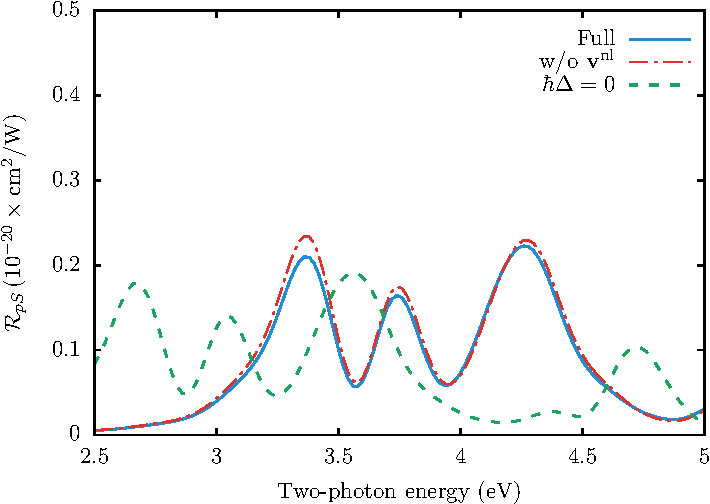
\includegraphics[width=0.7\textwidth]{content/figures/fig-4_4_03}
\caption{Calculated results for $\mathcal{R}_{pS}$ for the different levels of
approximation proposed in this article. All curves were calculated using the
3-layer model. We take $\theta=65^{\circ}$ for this plot. See text for full
details. All curves are broadened with $\sigma=0.075\,\text{eV}$.}
\label{fig:improvements}
\end{figure}


%%%%%%%%%%%%%%%%%%%%%%%%%%%%%%%%%%%%%%%%%%%%%%%%%%%%%%%%%%%%%%%%%%%%%%%%%%%%%%%%

\subsection{Calculated \texorpdfstring{$\mathcal{R}_{sP}$}{RsP} compared to 
experiment}\label{sec:1x1RsP}

Next, I analyze and compare the calculated $\mathcal{R}_{sP}$ spectra with
experimental data from Ref. \cite{mejiaPRB02}. The calculation adheres to the
experimental setup by taking an angle of incidence $\theta=65^{\circ}$ and an
azimuthal angle $\phi=30^\circ$. As seen in Fig. \ref{fig:RsP}, the overall
intensity of $\mathcal{R}_{sP}$ is one order of magnitude lower than
$\mathcal{R}_{pS}$. The experimental data is far noisier than in the other cases
but the E$_{1}$ and E$_{2}$ peaks are still discernible. As with the previous
comparisons, the 3-layer model is the closest match in both intensity and
lineshape to the experimental spectrum. It produces a curve that is very close
to the experimental intensity with good proportional heights for the calculated
E$_{1}$ and E$_{2}$ peaks. In contrast, the 2-layer-fresnel model is 100 times
more intense than experiment and produces an enlarged E$_{2}$ peak. The
2-layer-bulk model is ten times smaller with a very similar lineshape to the
3-layer model.

The differences between the 2-layer-fresnel and 2-layer-bulk models are not
derived from Eq. \eqref{eq:rsP}, as the $\varepsilon_{b}(2\omega)$ does not
change and the second term vanishes for this azimuthal angle of $\phi = 30$.
However, $\Gamma^{\ell}_{sP}$ does cause a significant change in the intensity
as there is an $\varepsilon_{\ell}(2\omega)$ term in the denominator. This will
become $\varepsilon_{v}(2\omega) = 1$ for the 2-layer-fresnel model, and
$\varepsilon_{b}(2\omega)$ in the bulk model. This accounts for the significant
difference between the intensity of the two models, while the lineshape remains
mostly consistent.

At higher energies, the theoretical curve is blueshifted as compared to the
experiment. The best explanation for this is the inclusion of the scissor
operator, which does not adequately correct the transitions occurring at these
higher energies. A full GW calculation would be well suited for this task, but
is well beyond the scope of this work.

\begin{figure}
\centering
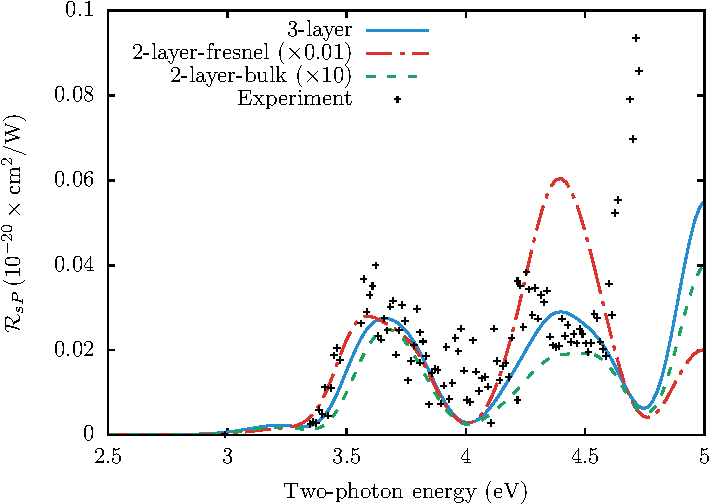
\includegraphics[width=0.7\textwidth]{content/figures/fig-4_4_04}
\caption{Comparison between theoretical models (see Table \ref{tab:models}) and
experiment for $\mathcal{R}_{sP}$, for $\theta=65^{\circ}$, and a scissors
value of $\hbar\Delta = 0.7\,\text{eV}$. All theoretical curves are broadened
with $\sigma=0.075\,\text{eV}$. Experimental data taken from Ref.
\cite{mejiaPRB02}, measured at room temperature.}
\label{fig:RsP}
\end{figure}


%%%%%%%%%%%%%%%%%%%%%%%%%%%%%%%%%%%%%%%%%%%%%%%%%%%%%%%%%%%%%%%%%%%%%%%%%%%%%%%%

\subsection{Calculated \texorpdfstring{$\mathcal{R}_{pP}$}{RpP} compared to
experiment}\label{sec:1x1RpP}

I present $\mathcal{R}_{pP}$ compared to experimental data from Ref.
\cite{mejiaPRB02} in Fig. \ref{fig:RpP}. Note that peak position for the 3-layer
model is similar to experiment with the overall intensity being only two times
larger. The E$_{2}$ peak is blueshifted by around 0.3\,eV, and the yield does
not go to zero after 4.75\,eV. The 2-layer-fresnel model produces a spectrum
with peak positions that are close to the experiment, but are 40 times more
intense. The calculated E$_{2}$ peak is similar, but the E$_{1}$ peak lacks the
sharpness present in the experiment. The 2-layer-bulk model is almost identical
in lineshape to the 3-layer model, but with eight times less intensity.

From Eq. \eqref{eq:rpP}, it is clear that $\mathcal{R}_{pP}$ has several
$2\omega$ terms that will change between models; this will have a deep effect on
the lineshape. Additionally, $\Gamma^{\ell}_{pP}$ also has
$\varepsilon_{\ell}(2\omega)$ in the denominator, and so we have a significant
difference in both lineshape and intensity between the 2-layer-fresnel and the
other two models. Again, as in the previous sections for $\mathcal{R}_{pS}$ and
$\mathcal{R}_{sP}$, the 3-layer model is the closest in intensity to the
experiment. Additionally, Ref. \cite{dadapPRB97} shows that low temperature
measurements of $\mathcal{R}_{pP}$ will blueshift the spectrum away from room
temperature measurements such as those shown in Figs. \ref{fig:RpP} and
\ref{fig:mitchellRpP}, and towards the theoretical results.

\begin{figure}
\centering 
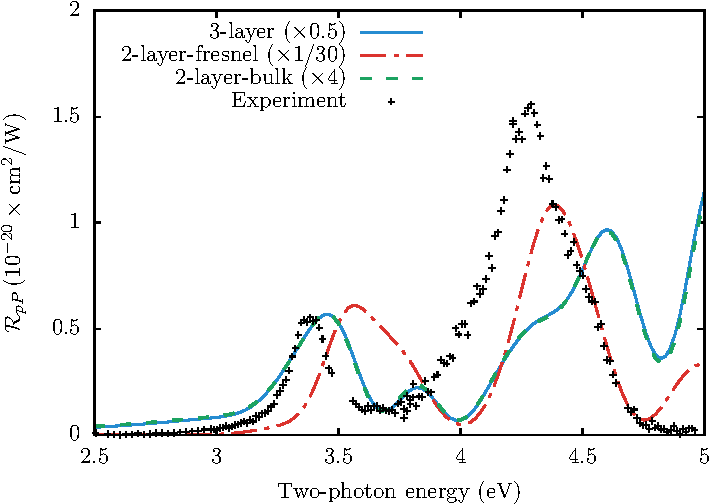
\includegraphics[width=0.7\textwidth]{content/figures/fig-4_4_05}
\caption{Comparison between theoretical models (see Table \ref{tab:models}) and
experiment for $\mathcal{R}_{pP}$, for $\theta=65^{\circ}$, and a scissors
value of $\hbar\Delta = 0.7\,\text{eV}$. All theoretical curves are broadened
with $\sigma=0.075\,\text{eV}$. Experimental data taken from Ref.
\cite{mejiaPRB02}, measured at room temperature.}
\label{fig:RpP}
\end{figure}

Reviewing Eq. \eqref{eq:rpP}, we see that $\mathcal{R}_{pP}$ is by far the most involved calculation, since it includes all four nonzero components. In particular, $\chi_{\perp\perp\perp}$ and $\chi_{\parallel\parallel\perp}$ include out-of-plane incoming fields. These are affected by local field effects\cite{tancognedejean:tel-01235611} that reveal the inhomogeneities in the material, which are by far more prevalent perpendicular to the surface than in the surface plane. This can be evidenced for Si, as Reflectance Anisotropy Spectroscopy (RAS) measurements are well described by \emph{ab initio} calculations neglecting local field effects.\cite{palummoPRB99, gaalPRB09} It is therefore expected that the out-of-plane components will be more sensitive to the inclusion of local fields. These will not change the transition energies, only their relative weights of the resonant peaks,\cite{tancognedejean:tel-01235611} but including these effects is challenging to compute,\cite{nicolasPRB15} and beyond the scope of this paper. We speculate that $\mathcal{R}_{pP}$ requires the proper inclusion of these effects in order to accurately describe the experimental peaks.

In Fig. \ref{fig:mitchellRpP}, I compare the theoretical spectra to results from
Ref. \cite{mitchellSS01}. The 3-layer model is, as before, close to the
experiment in both peak position and intensity. Intensity is almost the same the
experimental value. This provides a more compelling argument against the
2-layer-fresnel model than Fig. \ref{fig:RpP}. The 2-layer-fresnel model is 20
times more intense and blueshifted by around 0.1\,eV. As mentioned above, this
surface is of very high quality with measurements taken shortly after surface
preparation. The 2-layer-bulk model is intermediate between the other two models
in both intensity and lineshape. Under these conditions, the 3-layer model very
accurately reproduces the E$_{1}$ peak over the 2-layer-fresnel and 2-layer-bulk
models.

\begin{figure}
\centering
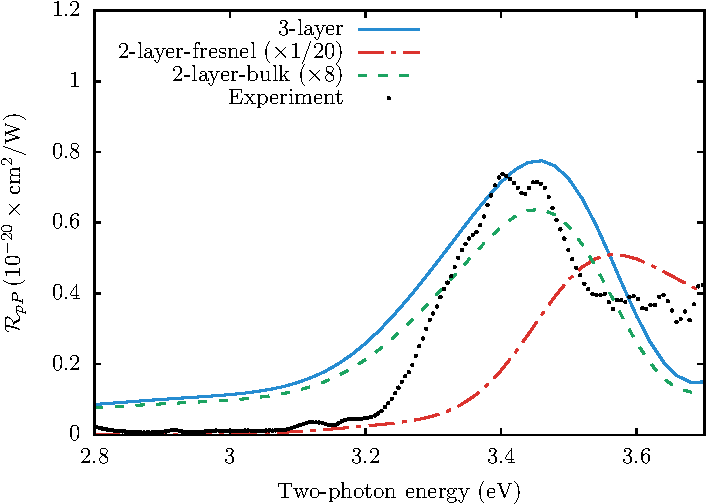
\includegraphics[width=0.7\textwidth]{content/figures/fig-4_4_06}
\caption{Comparison between theoretical models (see Table \ref{tab:models}) and
experiment for $\mathcal{R}_{pP}$, for $\theta=45^{\circ}$, and a scissors
value of $\hbar\Delta = 0.7\,\text{eV}$. All theoretical curves are broadened
with $\sigma=0.075\,\text{eV}$. Experimental data taken from Ref.
\cite{mitchellSS01}, measured at room temperature.}
\label{fig:mitchellRpP}
\end{figure}

I'll take this moment to present some auxiliary results from Sec. \ref{sec:scenarios} in Fig. \ref{fig:othermodels}. The 2-layer

\begin{figure}
\centering 
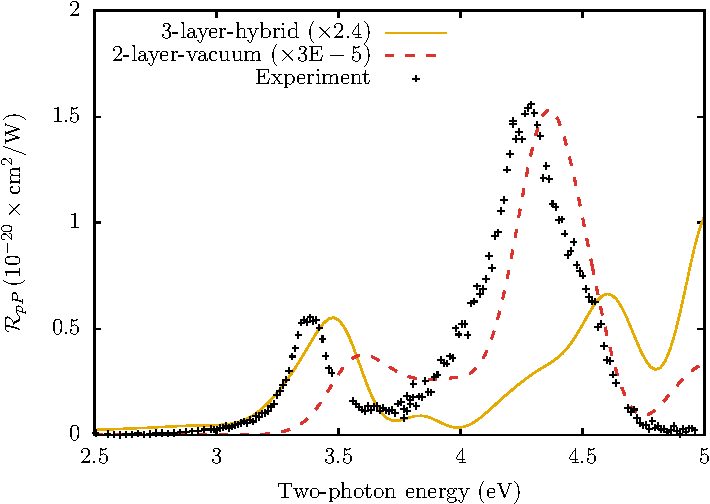
\includegraphics[width=0.7\textwidth]{content/figures/fig-4_4_07}
\caption{Other models. \label{fig:othermodels}}
\end{figure}

Lastly, for linear optics and SHG, $GW$ transition energies are needed. Doing a Bethe-Salpeter calculation for SSHG will improve the position and the amplitude of the peaks, but is far beyond current capabilities.\cite{puff} We did not adjust the value of the scissors shift, as we want to keep our calculation at the {\em ab initio} level. We remark again that the choice of $\hbar\Delta=0.7$ eV for the scissors shift comes from a $GW$ calculation.\cite{liPRB10} As explained in Fig. \ref{fig:improvements}, the lack of surface states causes an almost rigid shift of the spectra by applying the scissors correction. We have checked that it is not possible to have a single scissors value that can reproduce the energy positions of both the E$_{1}$ and the E$_{2}$ peaks. Of course, the experimental temperature at which the spectra is measured should be taken into account in a more complete formulation. However, we have restricted our calculation to $T=0$ K.


%%%%%%%%%%%%%%%%%%%%%%%%%%%%%%%%%%%%%%%%%%%%%%%%%%%%%%%%%%%%%%%%%%%%%%%%%%%%%%%%
\subsection{}

\begin{figure}
    \begin{minipage}[b]{0.5\textwidth}
        \centering
        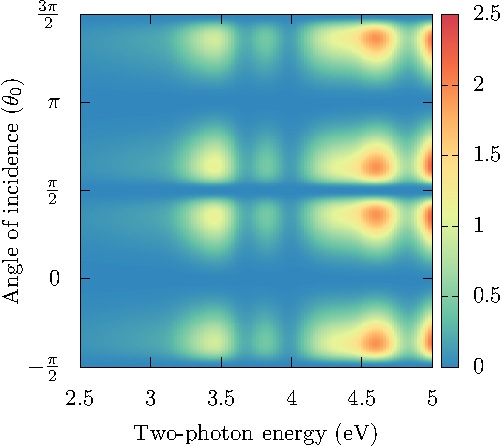
\includegraphics[height=6cm]{content/figures/fig-4_4_08}
        \subcaption{$\mathcal{R}_{pP}$}\label{fig:1x1rpp3d}
    \end{minipage}
    ~
    \begin{minipage}[b]{0.5\textwidth}
        \centering
        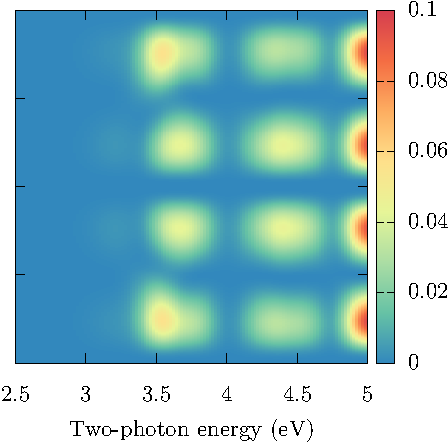
\includegraphics[height=5.945cm]{content/figures/fig-4_4_09}
        \subcaption{$\mathcal{R}_{sP}$}\label{fig:1x1rsp3d}
    \end{minipage}
    \caption{$\mathcal{R}$ for outgoing $P$ polarized fields, versus the angle
    of incidence ($\theta_{0}$) for the Si(111)(1$\times$1):H surface. Both
    figures consider an azimuthal angle of $\phi = 45^{\circ}$. All curves are
    broadened with $\sigma = 0.075$ eV.}
    \label{fig:1x1rP3d}
\end{figure}

\begin{figure}
    \begin{minipage}[b]{0.5\textwidth}
        \centering
        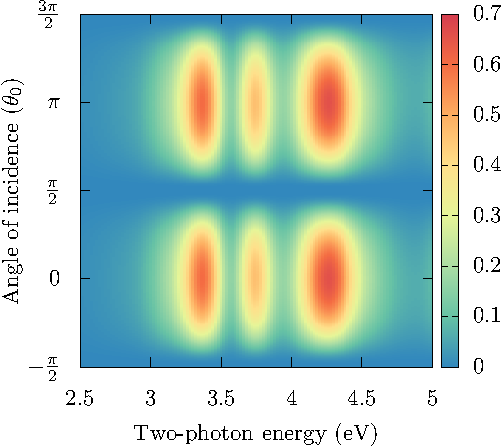
\includegraphics[height=6cm]{content/figures/fig-4_4_10}
        \subcaption{$\mathcal{R}_{pS}$}\label{fig:1x1rps3d}
    \end{minipage}
    ~
    \begin{minipage}[b]{0.5\textwidth}
        \centering
        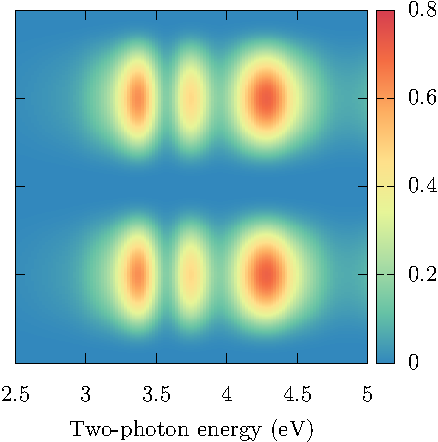
\includegraphics[height=5.945cm]{content/figures/fig-4_4_11}
        \subcaption{$\mathcal{R}_{sS}$}\label{fig:1x1rss3d}
    \end{minipage}
    \caption{$\mathcal{R}$ for outgoing $S$ polarized fields, versus the angle
    of incidence ($\theta_{0}$) for the Si(111)(1$\times$1):H surface. Both
    figures consider an azimuthal angle of $\phi = 45^{\circ}$. All curves are
    broadened with $\sigma = 0.075$ eV.}
    \label{fig:1x1rS3d}
\end{figure}


%%%%%%%%%%%%%%%%%%%%%%%%%%%%%%%%%%%%%%%%%%%%%%%%%%%%%%%%%%%%%%%%%%%%%%%%%%%%%%%%

\subsection{Calculating \texorpdfstring{$\mathcal{R}_{\mathrm{iF}}$}{Rif}
including the effects of multiple reflections}\label{sec:rifmr}

We consider a Si(111)(1$\times$1):H surface as a test case for the three layer model and to study the effects that multiple reflections have on the SSHG radiation. This surface is well characterized experimentally,\cite{mitchellSS01, mejiaPRB02, bergfeldPRL04} and there has been success in reproducing these experimental results using the three layer model without multiple reflections.\cite{andersonPRB16} The details of the \emph{ab initio} calculation of $\chi_{ijk}$ are not needed for the following discussion, and are left for the reader in Ref. \cite{andersonPRB16}. However, we mention that we apply a scissors shift of 0.7 eV to the theoretical spectra. In a first approximation, this includes the effects of the electronic many-body interactions within the independent particle approach for the \emph{ab initio} calculation. This 0.7 eV value allows the SH resonant peaks to acquire their corresponding energy positions, and is calculated with what is known as a $G_{0}W_{0}$ calculation.\cite{andersonPRB16} As mentioned in Sec. \ref{sec:intro}, we are interested in finding the thickness of the layer $\ell$ where $\chi_{ijk} \ne 0$. For this surface, we found well-converged results for a thickness of $\sim 5$ nm, that is equivalent to 24 atomic sheets of Si along the (111) direction. As this represents only the upper half of the slab, we find it reasonable to choose the thickness of the layer $\ell$ to be between $d\sim 5-10$ nm. This corresponds to a half-slab comprised of 24 to 48 atomic layers to get well-converged values of $\chi_{ijk}$.

We begin our comparisons in Fig. \ref{fig:average}, in which we compare the theoretical results for the SHG radiation with the experimental results from Ref. \cite{mejiaPRB02}. The theoretical curves that include multiple reflections are featured with the average value $\bar{R}^{M}_{i}$, Eq. \eqref{eq:mcave2}, with two values for the total thickness, $d$, and Eqs. \eqref{eq:mc78} and \eqref{rpp111}. We contrast these with the standard three layer model excluding the effects of multiple reflections from Sec. \ref{sec:nomr}. We see that the $E_{2}$ peak is blueshifted by around 0.3\,eV, and the yield does not go to zero after 4.75\,eV. $\mathcal{R}_{pP}$ is by far the most involved calculation out of the four different polarization cases, since it includes all four nonzero components. In particular, $\chi_{\perp\perp\perp}$ and $\chi_{\parallel\parallel\perp}$ include out-of-plane incoming fields. These are affected by local field effects that can change both intensity and peak position.\cite{tancognedejean:tel-01235611} Including these effects is computationally very expensive and is beyond the scope of this paper. We speculate that $\mathcal{R}_{pP}$ requires the proper inclusion of these effects in order to accurately describe the experimental peaks.

\begin{figure}
\centering
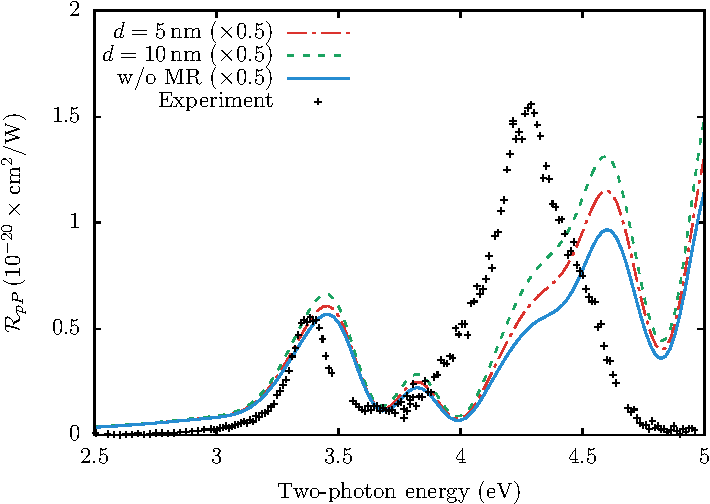
\includegraphics[width=0.7\textwidth]{content/figures/fig-4_4_12}
\caption{Comparison between the three layer model with the effects of multiple reflections for two different values of the total layer thickness $d$, with the standard three layer model without the effects of multiple reflections, and the experimental data from Ref. \cite{mejiaPRB02}. We take $\theta=65^{\circ}$, $\phi=30^{\circ}$, and a scissors value of $\hbar\Delta = 0.7\,\text{eV}$. The $\chi_{ijk}$ components are broadened with $\sigma=0.05\,\text{eV}$, and then $\mathcal{R}_{pP}$ is broadened with $\sigma=0.10\,\text{eV}$.}
\label{fig:average}
\end{figure}

\begin{figure}
\centering
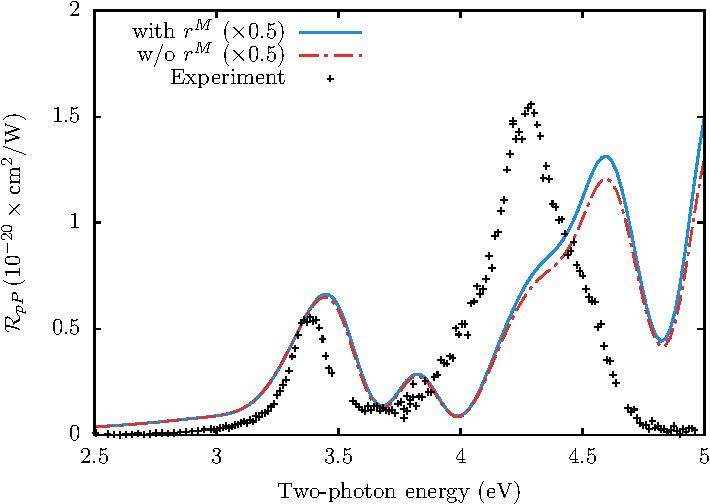
\includegraphics[width=0.7\textwidth]{content/figures/fig-4_4_13}
\caption{Comparison between theoretical models (see Table
\ref{tab:models}) and experiment for $\mathcal{R}_{pP}$, for
$\theta=45^{\circ}$, and a scissors value of $\hbar\Delta = 0.7\,\text{eV}$.
All theoretical curves are broadened with $\sigma=0.075\,\text{eV}$.
Experimental data taken from Ref. \cite{mitchellSS01}, measured at room
temperature.}
\label{fig:mr2}
\end{figure}

In Fig. \ref{fig:d2values}, we compare the theoretical results for the SSHG yield with the experimental results from Ref. \cite{mejiaPRB02}. We mention that the experimental results where produced with an angle of incidence of $\theta=65^\circ$, and an azimuthal angle of $\phi=30^\circ$, which eliminates the contribution from $\chi_{xxx}$ from Eq. \eqref{rpp111}. First, we note that the experimental spectrum shows two very well defined resonances which come from electronic transitions from the valence to the conduction bands around the well known $E_{1}\sim 3.4$ eV and $E_{2}\sim 4.3$ eV critical points of Si.\cite{yubook} As can be seen, the theoretical results reproduce the features of the spectrum, although we see that the $E_{2}$ peak is blueshifted by around 0.3\,eV. Here we focus on the SSHG yield itself rather than on the physics that lead to such a blueshifted theoretical spectrum. The interested reader can refer to Ref. \cite{andersonPRB16} for those details.

All curves in this figure that include multiple reflections consider $d = 10$ nm. We compare the theoretical SSHG yield for $d_{2} = 0$ nm and $d_{2} = 10$ nm, with the SSHG yield that neglects multiple reflections. When $d_{2} = 0$ nm, we have placed the polarization sheet at the bottom of the layer region. This minimizes the effect of the multiple reflections, and thus the curve is very similar to the three layer model that neglects multiple reflections entirely. When $d_{2} = 10$ nm, the polarization sheet is placed at the top of the layer region. This maximizes the effect of the multiple reflections and therefore leads to the largest yield. We also notice that the average value obtained by using $\bar{R}^{M}_{i}$ (Eq. \eqref{eq:mcave}) is intermediate between $d_{2} = 0$ and $d_{2} = 10$ nm, as expected. This is very similar to selecting $d_{2} = d/2$, which can be interpreted as placing the nonlinear polarization sheet $\mathbf{P}(\mathbf{r},t)$ at the middle of layer $\ell$. It is important to remark that these enhancements are larger for $E_{2}$ than for $E_{1}$. This can be understood from the fact that the corresponding $\lambda_{0}$ for $E_{1}$ is larger than that of $E_{2}$. From Eqs. \eqref{delta0}, \eqref{delta}, and \eqref{mphi}, we see that the phase shifts are larger for $E_{2}$ than for $E_{1}$, producing a larger enhancement of the SSHG yield at $E_{2}$ from the multiple reflections. As the phase shifts grow with $d$, so does the enhancement caused by the multiple reflections. We have verified that the effects of the multiple reflections from the linear field are significantly smaller than those of the SH field. This is clear since the phase shift of Eq. \eqref{mphi} is not only a factor of 2 smaller than that of Eqs. \eqref{delta0} and \eqref{delta}, but also $w_\ell < W_\ell$.

From this figure, it becomes evident that the inclusion of multiple reflections is crucial to obtain a better agreement between the theoretical SSHG yield and the experimental spectrum. This is particularly true for larger energies, such as $E_{2}$, as $\lambda_{0}$ becomes smaller and the multiple reflection effects become more noticeable. The selected value for $d << \lambda_{0}$, that comes naturally from the \emph{ab initio} calculation of $\chi_{ijk}$ is thus very reasonable in order to model a thin surface layer below the vacuum region where the nonlinear SH conversion takes place.

\begin{figure}
\centering
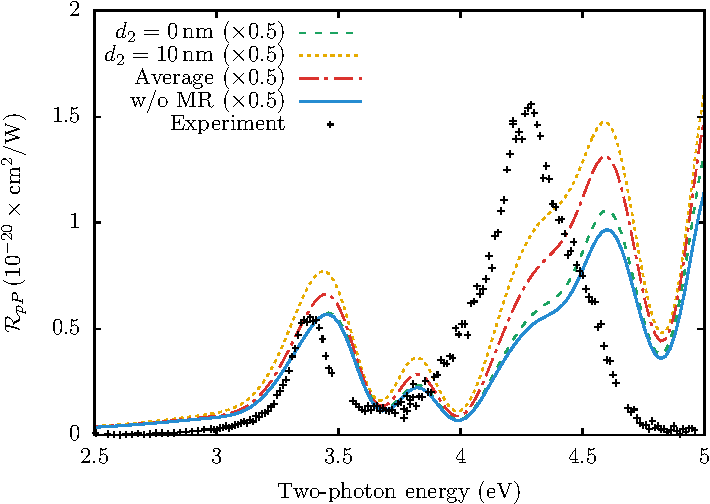
\includegraphics[width=0.7\textwidth]{content/figures/fig-4_4_14}
\caption{Comparison between the three layer model with the effects of multiple reflections for two different values of $d_{2}$, using the average value $\bar{R}^{M}_{i}$ Eq. of Eq. \eqref{eq:mcave2}, the three layer model without the effects of multiple reflections, and the experimental data from Ref. \cite{mejiaPRB02}. All curves that include multiple reflections consider a layer $\ell$ thickness of $d = 10\,\mathrm{nm}$.}
\label{fig:d2values}
\end{figure}

%!TEX root = ../../main.tex
\chapter{Final Remarks}\label{chap:conclusions}
\partialtoc


\section{Conclusions}


We have presented a formulation to calculate the surface second-harmonic (SSH)
susceptibility tensor $\boldsymbol{\chi}(-2\omega;\omega,\omega)$, using the
length gauge formalism and within the independent particle approximation (IPA).
It includes on equal footing: (i) the scissors correction, (ii) the contribution
of the non-local part of the pseudopotentials, and (iii) the cut function. We
have used a Si(001)$2\times 1$ surface to confirm that our scheme correctly
obtains the surface response as we confirm that
$\chi_{\mathrm{half-slab}}^{xxx}(-2\omega;\omega,\omega) \approx
\chi_{\mathrm{full-slab}}^{xxx}(-2\omega;\omega,\omega) . $ Although one can in
principle increase the number of atomic layers, $\mathbf{k}$-points, etc. to
improve even further on the similarity of the half-slab and full-slab results,
we have chosen a good compromise between accuracy and the burden and time of the
computations. We describe the effect of the independent inclusion of the three
effects mentioned above in the calculation of
$\boldsymbol{\chi}(-2\omega;\omega,\omega)$. The scissors correction shifts the
spectrum to higher energies though the shifting is not rigid and mixes the
$1\omega$ and $2\omega$ resonances, and has a strong influence in the
line-shape, as for the case of bulk
semiconductors.\cite{luppiJCP10,luppiPRB10,leitsmannPRB05} The cut function
allows us to extract unequivocally $\chi^{xxx}_{2\times
1}(-2\omega;\omega,\omega)$. The effects of the nonlocal part of the
pseudopotentials keeps the same line-shape of $|\chi^{xxx}_{2\times
1}(-2\omega;\omega,\omega)|$, but reduces the value of by 15-20\%. The $xxx$
component of $\boldsymbol{\chi}_{2\times 1}(-2\omega;\omega,\omega)$, can not be
experimentally isolated, however in a forthcoming publication we will compare
our formulation against experimental results. We have neglected local field and
excitonic effects. Although these are important factors in the optical response
of a semiconductor, their efficient calculation is theoretically and numerically
challenging and still under debate.\cite{beyond} This merits further study but
is beyond the scope of this paper. Nevertheless, the inclusion of aforementioned
contributions in our scheme opens the unprecedented possibility to study surface
SHG with more versatility and more accurate results.


We have presented new \emph{ab initio} LDA calculations for SSHG that are in
good quantitative agreement with experimental SSHG spectra for the
Si(111)(1$\times$1):H surface. These calculations include contributions not
previously considered in a single formulation, to wit, (i) the scissors
correction, (ii) the contribution of the nonlocal part of the pseudopotentials,
and (iii) the cut function used to extract the surface response, all within the
independent particle approximation. We also revised the 3-layer model for the
SSHG yield where the nonlinear polarization,
$\boldsymbol{\mathcal{P}}(2\omega)$, and the fundamental fields are taken within
a small layer $\ell$ below the surface of the material. This model reproduces
key spectral features and yields an intensity closer to the experiment for all
cases of $\mathcal{R}_{\mathrm{iF}}$. We consider it an upgrade over the much
reviewed 2-layer model\cite{mizrahiJOSA88}, and it comes with very little added
computational expense. Additionally, we have compared these two models with
another definition of the 2-layer model, where both
$\boldsymbol{\mathcal{P}}(2\omega)$ and the fundamental fields are considered
inside the bulk of the material. We found that this model yields an intensity
lower than the 3-layer model, but far closer than the 2-layer-vacuum model.
Lineshape is very similar between the 3-layer and 2-layer-bulk models.
Therefore, we consider that the 3-layer model offers the closest comparison to
experiment, while the 2-layer-bulk model offers a reasonable compromise between
the 3-layer and 2-layer-vacuum models.

This study affords us an interesting view of both the theoretical and
experimental aspects of SSHG studies. On the theoretical side, we have shown the
importance of using relaxed atomic positions to more accurately calculate the
nonlinear susceptibility tensor. The intensity of these spectra is greatly
improved when compared to previous works.\cite{mejiaPRB02} We also postulate
that the lack of local field effects in the theory is a serious shortcoming, but
in this case, it only affects two of the
$\boldsymbol{\chi}(-2\omega;\omega,\omega)$ components.

Concerning the experiments, we show that surface preparation and quality are
important for better results. The approach for calculating the SSHG yield
presented here finds closer agreement with surfaces that are freshly prepared
with little or no oxidation, and with measurements taken at low temperatures.

Overall, this newly implemented framework for calculating
$\boldsymbol{\chi}(-2\omega;\omega,\omega)$ and $\mathcal{R}$ focused on the
well-known Si(111)(1$\times$1):H surface provides a compelling benchmark for
SSHG studies. We are confident that this work can be applied directly to many
other surfaces of interest.

\section{Future Work}
I think that every work of experimental science has its fair share of setbacks,
complications, and difficulties. Sometimes the work itself can be very difficult
or even dangerous. Other times, the work is so cutting edge that problems have
to be solved as they come without the help of literature. Regardless of the
scope of the work, \emph{all} experimentation is very touch-and-go business --
you arm yourself with the best tools available for the job and hope for the
best. This work had its share of complications and setbacks, chief amongst these
was the constant breakdown of lasers in both countries. Then, the poor quality
of the samples which only came to light after they were in place and ready to be
measured. Lastly, the lack of information about the samples did not allow for
the systematic study needed to get the most out of this project.

Fortunately, Stephen Jay Gould once said that, ``Honorable errors do not count
as failures in science, but as seeds for progress in the quintessential activity
of correction.'' With that in mind I summarize what was learned from this.

First, the XP2SHG/SFG technique is fairly unique and specialized even amongst
groups that are dedicated to surface optics and nonlinear optical techniques.
Learning how this technique works and how it is used will be invaluable for
future work in this field. Actually having seen it in use, and then using it for
myself in the company of the people who pioneered it was a rewarding and
educational experience.

Second, while the results were inconclusive, the types of measurements done on
these types of samples are new and unexplored. There is much work to be done
with these kinds of materials and I hope that this work can serve as a starting
point for other interested scientists. I have no doubt in my mind that better
samples would have yielded excellent new results.

Lastly, this entire work helped broaden my knowledge of nonlinear optics in
general, as well as the many experimental techniques used everyday by scientists
everywhere. Even so, I only possess a very small portion of the ``big picture''
needed to understand every aspect of this work. There is still a lot to be
learned about surface optics and nonlinear techniques and I hope that this work,
at the very least, will pique the readers' interest on these topics.

\stopcontents[chapters]


\appendix
%!TEX root = ../../main.tex
\chapter{Useful derivations for the nonlinear surface susceptibility}
\label{app:chi2deriv}
\partialtoc




\stopcontents[chapters]

% %!TEX root = ../../main.tex
\chapter{Miscellaneous Results for the Nonlinear Surface susceptibility}
\partialtoc


%%%%%%%%%%%%%%%%%%%%%%%%%%%%%%%%%%%%%%%%%%%%%%%%%%%%%%%%%%%%%%%%%%%%%%%%%%%%%%%%
%%%%%%%%%%%%%%%%%%%%%%%%%%%%%%%%%%%%%%%%%%%%%%%%%%%%%%%%%%%%%%%%%%%%%%%%%%%%%%%%

\section{Divergence Free Expressions for $\chi^s_{\mathrm{a}\mathrm{b}\mathrm{c}}$}

We add the $\mathbf{k}$ and $-\mathbf{k}$ terms of expressions \eqref{pfe} and
\eqref{pfi} to obtain:
\begin{align}\label{chi1}
A
\left[
-\frac{1}{2\omega_{lm}(2\omega_{lm}-\omega_{nm})}\frac{1}{\omega_{lm}-\omega}
\right]&=-\frac{f_{ml}}{2}
\left[
\frac{\mathcal{P}^{\mathrm{a}}_{mn}r^{\mathrm{c}}_{nl}r^{\mathrm{b}}_{lm}}{\omega_{lm}(2\omega_{lm}-\omega_{nm})}\frac{1}{\omega_{lm}-\omega}|_{\mathbf{k}}
\right.
\nonumber\\
+
\left.
\frac{\mathcal{P}^{\mathrm{a}}_{mn}r^{\mathrm{c}}_{nl}r^{\mathrm{b}}_{lm}}{\omega_{lm}(2\omega_{lm}-\omega_{nm})}\frac{1}{\omega_{lm}-\omega}|_{-\mathbf{k}}
\right]
&=-\frac{f_{ml}}{2}
\left[
\frac{\mathcal{P}^{\mathrm{a}}_{mn}r^{\mathrm{c}}_{nl}r^{\mathrm{b}}_{lm}}{\omega_{lm}(2\omega_{lm}-\omega_{nm})}\frac{1}{\omega_{lm}-\omega}|_{\mathbf{k}}
\right.
\nonumber\\
-
\left.
\frac{\mathcal{P}^{\mathrm{a}}_{nm}r^{\mathrm{c}}_{ln}r^{\mathrm{b}}_{ml}}{\omega_{lm}(2\omega_{lm}-\omega_{nm})}\frac{1}{\omega_{lm}-\omega}|_{\mathbf{k}}
\right]
&=-\frac{f_{ml}}{2}
\frac{1}{\omega_{lm}(2\omega_{lm}-\omega_{nm})}\frac{1}{\omega_{lm}-\omega}
\nonumber\\
&\times&
\left[
\mathcal{P}^{\mathrm{a}}_{mn}r^{\mathrm{c}}_{nl}r^{\mathrm{b}}_{lm}
-
\mathcal{P}^{\mathrm{a}}_{nm}r^{\mathrm{c}}_{ln}r^{\mathrm{b}}_{ml}
\right]
\\
=-\frac{f_{ml}}{2}
\frac{1}{\omega_{lm}(2\omega_{lm}-\omega_{nm})}\frac{1}{\omega_{lm}-\omega}
\left[
\mathcal{P}^{\mathrm{a}}_{mn}r^{\mathrm{c}}_{nl}r^{\mathrm{b}}_{lm}
-
(\mathcal{P}^{\mathrm{a}}_{mn}r^{\mathrm{c}}_{nl}r^{\mathrm{b}}_{lm})^*
\right]
&=-\frac{f_{ml}}{2}
\frac{2i\mathrm{Im}[\mathcal{P}^{\mathrm{a}}_{mn}r^{\mathrm{c}}_{nl}r^{\mathrm{b}}_{lm}]}{\omega_{lm}(2\omega_{lm}-\omega_{nm})}\frac{1}{\omega_{lm}-\omega}
\nonumber
,
\end{align}
where we used the Hermiticity of the momentum and position operators.
Likewise we get that
\begin{align}\label{si}
A
\left[
\frac{2}{\omega_{nm}(2\omega_{lm}-\omega_{nm})}\frac{1}{\omega_{nm}-2\omega}
\right]&=
f_{ml}
\frac{4i\mathrm{Im}[\mathcal{P}^{\mathrm{a}}_{mn}r^{\mathrm{c}}_{nl}r^{\mathrm{b}}_{lm}]}{\omega_{nm}(2\omega_{lm}-\omega_{nm})}\frac{1}{\omega_{nm}-2\omega}
.
\end{align}
Also,
\begin{align}\label{is}
&-
f_{ln}\mathcal{P}^{\mathrm{a}}_{mn}r^{\mathrm{b}}_{nl}r^{\mathrm{c}}_{lm}
\left[
-\frac{1}{2\omega_{nl}(2\omega_{nl}-\omega_{nm})}\frac{1}{\omega_{nl}-\omega}
+\frac{2}{\omega_{nm}(2\omega_{nl}-\omega_{nm})}\frac{1}{\omega_{nm}-2\omega}
\right]
\nonumber\\
&=
-
2if_{ln}\mathrm{Im}[\mathcal{P}^{\mathrm{a}}_{mn}r^{\mathrm{b}}_{nl}r^{\mathrm{c}}_{lm}]
\left[
-\frac{1}{2\omega_{nl}(2\omega_{nl}-\omega_{nm})}\frac{1}{\omega_{nl}-\omega}
+\frac{2}{\omega_{nm}(2\omega_{nl}-\omega_{nm})}\frac{1}{\omega_{nm}-2\omega}
\right]
,
\end{align}
and therefore
\begin{align}\label{pfen}  
E&=  
2if_{ml}\mathrm{Im}[\mathcal{P}^{\mathrm{a}}_{mn}r^{\mathrm{c}}_{nl}r^{\mathrm{b}}_{lm}] 
\left[
-\frac{1}{2\omega_{lm}(2\omega_{lm}-\omega_{nm})}\frac{1}{\omega_{lm}-\omega}
+\frac{2}{\omega_{nm}(2\omega_{lm}-\omega_{nm})}\frac{1}{\omega_{nm}-2\omega}
\right]
\nonumber\\
&- 
2if_{ln}\mathrm{Im}[\mathcal{P}^{\mathrm{a}}_{mn}r^{\mathrm{b}}_{nl}r^{\mathrm{c}}_{lm}]
\left[
-\frac{1}{2\omega_{nl}(2\omega_{nl}-\omega_{nm})}\frac{1}{\omega_{nl}-\omega}
+\frac{2}{\omega_{nm}(2\omega_{nl}-\omega_{nm})}\frac{1}{\omega_{nm}-2\omega}
\right]
.
\end{align}  
Using above results into Eq.~\eqref{chie} implies
\begin{align}\label{pfen3} 
\chi_{e,\mathrm{a}\mathrm{b}\mathrm{c}}^{s,\ell}
&= 
-\frac{2e^3}{m_e\hbar^2} 
\sum_{\ell m n\mathbf{k}}
\left[ 
f_{ml}\mathrm{Im}[\mathcal{P}^{\mathrm{a}}_{mn}r^{\mathrm{c}}_{nl}r^{\mathrm{b}}_{lm}] 
\left[
-\frac{1}{2\omega_{lm}(2\omega_{lm}-\omega_{nm})}\frac{1}{\omega_{lm}-\omega}
+\frac{2}{\omega_{nm}(2\omega_{lm}-\omega_{nm})}\frac{1}{\omega_{nm}-2\omega}
\right]
\right.
\nonumber\\
&-
\left. 
f_{ln}\mathrm{Im}[\mathcal{P}^{\mathrm{a}}_{mn}r^{\mathrm{b}}_{nl}r^{\mathrm{c}}_{lm}]
\left[
-\frac{1}{2\omega_{nl}(2\omega_{nl}-\omega_{nm})}\frac{1}{\omega_{nl}-\omega}
+\frac{2}{\omega_{nm}(2\omega_{nl}-\omega_{nm})}\frac{1}{\omega_{nm}-2\omega}
\right]
\right]
\nonumber\\
&= 
-\frac{2e^3}{m_e\hbar^2} 
\sum_{\ell m n\mathbf{k}}
\left[ 
f_{ml}\mathrm{Im}[\mathcal{P}^{\mathrm{a}}_{mn}\{r^{\mathrm{c}}_{nl}r^{\mathrm{b}}_{lm}\}] 
\left[
-\frac{1}{2\omega_{lm}(2\omega_{lm}-\omega_{nm})}\frac{1}{\omega_{lm}-\omega}
+\frac{2}{\omega_{nm}(2\omega_{lm}-\omega_{nm})}\frac{1}{\omega_{nm}-2\omega}
\right]
\right.
\nonumber\\
&-
\left. 
f_{ln}\mathrm{Im}[\mathcal{P}^{\mathrm{a}}_{mn}\{r^{\mathrm{b}}_{nl}r^{\mathrm{c}}_{lm}\}]
\left[
-\frac{1}{2\omega_{nl}(2\omega_{nl}-\omega_{nm})}\frac{1}{\omega_{nl}-\omega}
+\frac{2}{\omega_{nm}(2\omega_{nl}-\omega_{nm})}\frac{1}{\omega_{nm}-2\omega}
\right]
\right]
,
\end{align}  
where $\{\}$ is the symmetrization of the Cartesian indices $\mathrm{b}\mathrm{c}$, i.e. 
$\{u^{\mathrm{b}}s^{\mathrm{c}}\}=(u^{\mathrm{b}}s^{\mathrm{c}}+u^{\mathrm{c}}s^{\mathrm{b}})/2$. 
Then, we see that
$\chi_{e,\mathrm{a}\mathrm{b}\mathrm{c}}^{s,\ell}=\chi_{e,acb}^{s,\ell}$. We further simplify 
the last equation as follows:
\begin{align}\label{pfen2} 
\chi_{e,\mathrm{a}\mathrm{b}\mathrm{c}}^{s,\ell}
&= 
-\frac{2e^3}{2m_e\hbar^2} 
\sum_{\ell m n\mathbf{k}}
\left[
\left[
-\frac{f_{ml}\mathrm{Im}[\mathcal{P}^{\mathrm{a}}_{mn}\{r^{\mathrm{c}}_{nl}r^{\mathrm{b}}_{lm}\}]}
{2\omega_{lm}(2\omega_{lm}-\omega_{nm})}\frac{1}{\omega_{lm}-\omega}
+\frac{2 f_{ml}\mathrm{Im}[\mathcal{P}^{\mathrm{a}}_{mn}\{r^{\mathrm{c}}_{nl}r^{\mathrm{b}}_{lm}\}]}
{\omega_{nm}(2\omega_{lm}-\omega_{nm})}\frac{1}{\omega_{nm}-2\omega}
\right]
\right.
\nonumber\\
&+
\left.
\left[
\frac{f_{ln}\mathrm{Im}[\mathcal{P}^{\mathrm{a}}_{mn}\{r^{\mathrm{b}}_{nl}r^{\mathrm{c}}_{lm}\}]}
{2\omega_{nl}(2\omega_{nl}-\omega_{nm})}\frac{1}{\omega_{nl}-\omega}
-\frac{2 f_{ln}\mathrm{Im}[\mathcal{P}^{\mathrm{a}}_{mn}\{r^{\mathrm{b}}_{nl}r^{\mathrm{c}}_{lm}\}]
}{\omega_{nm}(2\omega_{nl}-\omega_{nm})}\frac{1}{\omega_{nm}-2\omega}
\right]
\right]
\nonumber\\
&=
-\frac{2e^3}{m_e\hbar^2} 
\sum_{\ell m n\mathbf{k}}
\left[
\left[
\frac{2 f_{ml}\mathrm{Im}[\mathcal{P}^{\mathrm{a}}_{mn}\{r^{\mathrm{c}}_{nl}r^{\mathrm{b}}_{lm}\}]}
{\omega_{nm}(2\omega_{lm}-\omega_{nm})}
-\frac{2 f_{ln}\mathrm{Im}[\mathcal{P}^{\mathrm{a}}_{mn}\{r^{\mathrm{b}}_{nl}r^{\mathrm{c}}_{lm}\}]
}{\omega_{nm}(2\omega_{nl}-\omega_{nm})}
\right]
\frac{1}{\omega_{nm}-2\omega}
\right.
\nonumber\\
&+
\left.
\left[
\frac{f_{ln}\mathrm{Im}[\mathcal{P}^{\mathrm{a}}_{mn}\{r^{\mathrm{b}}_{nl}r^{\mathrm{c}}_{lm}\}]}
{2\omega_{nl}(2\omega_{nl}-\omega_{nm})}\frac{1}{\omega_{nl}-\omega}
-\frac{f_{ml}\mathrm{Im}[\mathcal{P}^{\mathrm{a}}_{mn}\{r^{\mathrm{c}}_{nl}r^{\mathrm{b}}_{lm}\}]}
{2\omega_{lm}(2\omega_{lm}-\omega_{nm})}
\frac{1}{\omega_{lm}-\omega}|_{\ell\leftrightarrow m}
\right]
\right]
\nonumber\\
&=
-\frac{e^3}{m_e\hbar^2} 
\sum_{\ell m n\mathbf{k}}
\left[
\left[
\frac{2 f_{ml}\mathrm{Im}[\mathcal{P}^{\mathrm{a}}_{mn}\{r^{\mathrm{c}}_{nl}r^{\mathrm{b}}_{lm}\}]}
{\omega_{nm}(2\omega_{lm}-\omega_{nm})}
-\frac{2 f_{ln}\mathrm{Im}[\mathcal{P}^{\mathrm{a}}_{mn}\{r^{\mathrm{b}}_{nl}r^{\mathrm{c}}_{lm}\}]
}{\omega_{nm}(2\omega_{nl}-\omega_{nm})}
\right]
\frac{1}{\omega_{nm}-2\omega}
\right.
\nonumber\\
&+
\left.
\left[
\frac{f_{ln}\mathrm{Im}[\mathcal{P}^{\mathrm{a}}_{mn}\{r^{\mathrm{b}}_{nl}r^{\mathrm{c}}_{lm}\}]}
{2\omega_{nl}(2\omega_{nl}-\omega_{nm})}\frac{1}{\omega_{nl}-\omega}
-\frac{f_{lm}\mathrm{Im}[\mathcal{P}^{\mathrm{a}}_{ln}\{r^{\mathrm{c}}_{nm}r^{\mathrm{b}}_{ml}\}]}
{2\omega_{ml}(2\omega_{ml}-\omega_{nl})}\frac{1}{\omega_{ml}-\omega}|_{n\leftrightarrow m}
\right]
\right]
\nonumber\\
&=
-\frac{e^3}{m_e\hbar^2} 
\sum_{\ell m n\mathbf{k}}
\left[
\left[
\frac{2 f_{ml}\mathrm{Im}[\mathcal{P}^{\mathrm{a}}_{mn}\{r^{\mathrm{c}}_{nl}r^{\mathrm{b}}_{lm}\}]}
{\omega_{nm}(2\omega_{lm}-\omega_{nm})}
-\frac{2 f_{ln}\mathrm{Im}[\mathcal{P}^{\mathrm{a}}_{mn}\{r^{\mathrm{b}}_{nl}r^{\mathrm{c}}_{lm}\}]
}{\omega_{nm}(2\omega_{nl}-\omega_{nm})}
\right]
\frac{1}{\omega_{nm}-2\omega}
\right.
\nonumber\\
&+
\left.
\left[
\frac{f_{ln}\mathrm{Im}[\mathcal{P}^{\mathrm{a}}_{mn}\{r^{\mathrm{b}}_{nl}r^{\mathrm{c}}_{lm}\}]}
{2\omega_{nl}(2\omega_{nl}-\omega_{nm})}\frac{1}{\omega_{nl}-\omega}
-\frac{f_{ln}\mathrm{Im}[\mathcal{P}^{\mathrm{a}}_{lm}\{r^{\mathrm{c}}_{mn}r^{\mathrm{b}}_{nl}\}]}
{2\omega_{nl}(2\omega_{nl}-\omega_{ml})}\frac{1}{\omega_{nl}-\omega}
\right]
\right]
\nonumber\\
&=
-\frac{e^3}{m_e\hbar^2} 
\sum_{\ell m n\mathbf{k}}
\left[
\left[
\frac{2 f_{ml}\mathrm{Im}[\mathcal{P}^{\mathrm{a}}_{mn}\{r^{\mathrm{c}}_{nl}r^{\mathrm{b}}_{lm}\}]}
{\omega_{nm}(2\omega_{lm}-\omega_{nm})}
-\frac{2 f_{ln}\mathrm{Im}[\mathcal{P}^{\mathrm{a}}_{mn}\{r^{\mathrm{b}}_{nl}r^{\mathrm{c}}_{lm}\}]
}{\omega_{nm}(2\omega_{nl}-\omega_{nm})}
\right]
\frac{1}{\omega_{nm}-2\omega}
\right.
\nonumber\\
&+
\left. 
f_{ln}
\left[
\frac{\mathrm{Im}[\mathcal{P}^{\mathrm{a}}_{mn}\{r^{\mathrm{b}}_{nl}r^{\mathrm{c}}_{lm}\}]}
{2\omega_{nl}(2\omega_{nl}-\omega_{nm})}
-\frac{f_{ln}\mathrm{Im}[\mathcal{P}^{\mathrm{a}}_{lm}\{r^{\mathrm{c}}_{mn}r^{\mathrm{b}}_{nl}\}]}
{2\omega_{nl}(2\omega_{nl}-\omega_{ml})}
\right]\frac{1}{\omega_{nl}-\omega}
\right]
,
\end{align}  
where the 2 in the denominator of the prefactor after the first equal
sign comes from the $\mathbf{k}$ and $-\mathbf{k}$ addition, i.e. 
$\chi\to\sum_{\mathbf{k}>0}[\chi(\mathbf{k})+\chi(-\mathbf{k})]/2$. 
Taking $\omega\to\omega +i\eta$ and use
$\lim_{\eta\to 0}1/(x-i\eta)=P(1/x)+i\pi\delta(x)$, to get
\begin{align}\label{imchie}
\mathrm{Im}[\chi_{e,\mathrm{a}\mathrm{b}\mathrm{c}}^{s,\ell}]
&=
\frac{2\pi e^3}{m_e\hbar^2} 
\sum_{\ell m n\mathbf{k}}
\left[
\left[
\frac{2 f_{ln}\mathrm{Im}[\mathcal{P}^{\mathrm{a}}_{mn}\{r^{\mathrm{b}}_{nl}r^{\mathrm{c}}_{lm}\}]
}{\omega_{nm}(2\omega_{nl}-\omega_{nm})}
-\frac{2 f_{ml}\mathrm{Im}[\mathcal{P}^{\mathrm{a}}_{mn}\{r^{\mathrm{c}}_{nl}r^{\mathrm{b}}_{lm}\}]}
{\omega_{nm}(2\omega_{lm}-\omega_{nm})}
\right]
\delta(\omega_{nm}-2\omega)
\right.
\nonumber\\
&+
\left. 
f_{ln}
\left[
\frac{\mathrm{Im}[\mathcal{P}^{\mathrm{a}}_{lm}\{r^{\mathrm{c}}_{mn}r^{\mathrm{b}}_{nl}\}]}
{2\omega_{nl}(2\omega_{nl}-\omega_{ml})}
-
\frac{\mathrm{Im}[\mathcal{P}^{\mathrm{a}}_{mn}\{r^{\mathrm{b}}_{nl}r^{\mathrm{c}}_{lm}\}]}
{2\omega_{nl}(2\omega_{nl}-\omega_{nm})}
\right]
\delta(\omega_{nl}-\omega)
\right]
.
\end{align}  
We change $l\leftrightarrow m$ in the last term,
to write
\begin{align}\label{imchie2}
\mathrm{Im}[\chi_{e,\mathrm{a}\mathrm{b}\mathrm{c}}^{s,\ell}]
&=
\frac{\pi e^3}{m_e\hbar^2} 
\sum_{\ell m n\mathbf{k}}
\left[
\left[
\frac{2 f_{ln}\mathrm{Im}[\mathcal{P}^{\mathrm{a}}_{mn}\{r^{\mathrm{b}}_{nl}r^{\mathrm{c}}_{lm}\}]
}{\omega_{nm}(2\omega_{nl}-\omega_{nm})}
-\frac{2 f_{ml}\mathrm{Im}[\mathcal{P}^{\mathrm{a}}_{mn}\{r^{\mathrm{c}}_{nl}r^{\mathrm{b}}_{lm}\}]}
{\omega_{nm}(2\omega_{lm}-\omega_{nm})}
\right]
\delta(\omega_{nm}-2\omega)
\right.
\nonumber\\
&+
\left. 
f_{mn}
\left[
\frac{\mathrm{Im}[\mathcal{P}^{\mathrm{a}}_{ml}\{r^{\mathrm{c}}_{ln}r^{\mathrm{b}}_{nm}\}]}
{2\omega_{nm}(2\omega_{nm}-\omega_{lm})}
-
\frac{\mathrm{Im}[\mathcal{P}^{\mathrm{a}}_{ln}\{r^{\mathrm{b}}_{nm}r^{\mathrm{c}}_{ml}\}]}
{2\omega_{nm}(2\omega_{nm}-\omega_{nl})}
\right]
\delta(\omega_{nm}-\omega)
\right]
.
\end{align}  
From the delta functions it follows that $n=c$ and $m=v$, then
$f_{ln}=1$ with $l=v'$,
$f_{ml}=1$ with $l=c'$, 
and
$f_{mn}=1$ with $l=c'$ or $v'$, and
\begin{align}\label{imchie3}
\mathrm{Im}[\chi_{e,\mathrm{a}\mathrm{b}\mathrm{c}}^{s,\ell}]
&=
\frac{\pi e^3}{m_e\hbar^2} 
\sum_{vc\mathbf{k}}
\left[
\left[
\sum_{v'\ne v}
\frac{2\mathrm{Im}[\mathcal{P}^{\mathrm{a},\ell}_{vc}\{r^{\mathrm{b}}_{cv'}r^{\mathrm{c}}_{v'v}\}]
}{\omega_{cv}(2\omega_{cv'}-\omega_{cv})}
-
\sum_{c'\ne c}
\frac{2\mathrm{Im}[\mathcal{P}^{\mathrm{a},\ell}_{vc}\{r^{\mathrm{c}}_{cc'}r^{\mathrm{b}}_{c'v}\}]}
{\omega_{cv}(2\omega_{c'v}-\omega_{cv})}
\right]
\delta(\omega_{cv}-2\omega)
\right.
\nonumber\\
&+
\left.
\sum_{l\neq(v,c)}
\left[
\frac{\mathrm{Im}[\mathcal{P}^{\mathrm{a},\ell}_{vl}\{r^{\mathrm{c}}_{lc}r^{\mathrm{b}}_{cv}\}]}
{2\omega_{cv}(2\omega_{cv}-\omega_{lv})}
-
\frac{\mathrm{Im}[\mathcal{P}^{\mathrm{a},\ell}_{lc}\{r^{\mathrm{b}}_{cv}r^{\mathrm{c}}_{vl}\}]}
{2\omega_{cv}(2\omega_{cv}-\omega_{cl})}
\right]
\delta(\omega_{cv}-\omega)
\right]
,
\end{align}  
where we put the layer $\ell$ dependence in $\mathcal{P}$.
Using Eq.~\eqref{rcal}, we can obtain the following result
\begin{align}\label{ptor}
2i\mathrm{Im}[\mathcal{P}^{\mathrm{a},\ell}_{nm}\{r^{\mathrm{b}}_{ml}r^{\mathrm{c}}_{ln}\}]
&=
\mathcal{P}^{\mathrm{a},\ell}_{nm}\{r^{\mathrm{b}}_{ml}r^{\mathrm{c}}_{ln}\}
-
(\mathcal{P}^{\mathrm{a},\ell}_{nm}\{r^{\mathrm{b}}_{ml}r^{\mathrm{c}}_{ln}\})^*
\nonumber\\
&=
im_e\omega_{nm}\mathcal{R}^{\mathrm{a},\ell}_{nm}\{r^{\mathrm{b}}_{ml}r^{\mathrm{c}}_{ln}\}
-
(im_e\omega_{nm}\mathcal{R}^{\mathrm{a},\ell}_{nm}\{r^{\mathrm{b}}_{ml}r^{\mathrm{c}}_{ln}\})^*
\nonumber\\
&=
im_e\omega_{nm}\left(\mathcal{R}^{\mathrm{a},\ell}_{nm}\{r^{\mathrm{b}}_{ml}r^{\mathrm{c}}_{ln}\}
+
(\mathcal{R}^{\mathrm{a},\ell}_{nm}\{r^{\mathrm{b}}_{ml}r^{\mathrm{c}}_{ln}\})^*
\right)
\nonumber\\
&=
2im_e\omega_{nm}\mathrm{Re}[\mathcal{R}^{\mathrm{a},\ell}_{nm}\{r^{\mathrm{b}}_{ml}r^{\mathrm{c}}_{ln}\}]
,
\end{align}
then, using $\omega_{vc}=-\omega_{vc}$ we obtain
\begin{align}\label{imchie3n}
\mathrm{Im}[\chi_{e,\mathrm{a}\mathrm{b}\mathrm{c}}^{s,\ell}]
&=
\frac{\pi e^3}{\hbar^2} 
\sum_{vc\mathbf{k}}
\left[
\left[
-\sum_{v'\ne v}
\frac{2\mathrm{Re}[\mathcal{R}^{\mathrm{a},\ell}_{vc}\{r^{\mathrm{b}}_{cv'}r^{\mathrm{c}}_{v'v}\}]
}{2\omega_{cv'}-\omega_{cv}}
+
\sum_{c'\ne c}
\frac{2\mathrm{Re}[\mathcal{R}^{\mathrm{a},\ell}_{vc}\{r^{\mathrm{c}}_{cc'}r^{\mathrm{b}}_{c'v}\}]}
{2\omega_{c'v}-\omega_{cv}}
\right]
\delta(\omega_{cv}-2\omega)
\right.
\nonumber\\
&+
\left.
\sum_{l\neq(v,c)}
\left[
\frac{\omega_{vl}\mathrm{Re}[\mathcal{R}^{\mathrm{a},\ell}_{vl}\{r^{\mathrm{c}}_{lc}r^{\mathrm{b}}_{cv}\}]}
{2\omega_{cv}(2\omega_{cv}-\omega_{lv})}
-
\frac{\omega_{lc}\mathrm{Re}[\mathcal{R}^{\mathrm{a},\ell}_{lc}\{r^{\mathrm{b}}_{cv}r^{\mathrm{c}}_{vl}\}]}
{2\omega_{cv}(2\omega_{cv}-\omega_{cl})}
\right]
\delta(\omega_{cv}-\omega)
\right]
.
\end{align}  
Finally, following Ref.~\cite{nastosPRB05, cabellosPRB09} we simply change
$\omega_{nm}\to\omega_{nm}^S$ to obtain the scissored expresion of
\begin{align}\label{imchies}
\mathrm{Im}[\chi_{e,\mathrm{a}\mathrm{b}\mathrm{c}}^{s,\ell}]
&=
\frac{\pi e^3}{2\hbar^2} 
\sum_{vc\mathbf{k}}
\left[
4
\left[
-\sum_{v'\ne v}
\frac{\mathrm{Re}[\mathcal{R}^{\mathrm{a},\ell}_{vc}\{r^{\mathrm{b}}_{cv'}r^{\mathrm{c}}_{v'v}\}]
}{2\omega^S_{cv'}-\omega^S_{cv}}
+
\sum_{c'\ne c}
\frac{\mathrm{Re}[\mathcal{R}^{\mathrm{a},\ell}_{vc}\{r^{\mathrm{c}}_{cc'}r^{\mathrm{b}}_{c'v}\}]}
{2\omega^S_{c'v}-\omega^S_{cv}}
\right]
\delta(\omega^S_{cv}-2\omega)
\right.
\nonumber\\
&+
\left.
\sum_{l\neq(v,c)}
\left[
\frac{\omega^S_{vl}\mathrm{Re}[\mathcal{R}^{\mathrm{a},\ell}_{vl}\{r^{\mathrm{c}}_{lc}r^{\mathrm{b}}_{cv}\}]}
{\omega^S_{cv}(2\omega^S_{cv}-\omega^S_{lv})}
-
\frac{\omega^S_{lc}\mathrm{Re}[\mathcal{R}^{\mathrm{a},\ell}_{lc}\{r^{\mathrm{b}}_{cv}r^{\mathrm{c}}_{vl}\}]}
{\omega^S_{cv}(2\omega^S_{cv}-\omega^S_{cl})}
\right]
\delta(\omega^S_{cv}-\omega)
\right]
,
\end{align}  
where we have ``pulled'' a factor of 1/2, so the prefactor is the same
as that of the velocity gauge formalism.\cite{cabellosPRB09} 
For the $I$ term of Eq.~\eqref{pfi}, we notice that the energy
denominators are invariant under $\mathbf{k}\to -\mathbf{k}$, and then we only
look at the numerators, then
\begin{align}\label{ct}
C\to f_{mn}\mathcal{P}^{\mathrm{a}}_{mn}(r^{\mathrm{b}}_{nm})_{;k^{\mathrm{c}}}|_{\mathbf{k}}
+
f_{mn}\mathcal{P}^{\mathrm{a}}_{mn}(r^{\mathrm{b}}_{nm})_{;k^{\mathrm{c}}}|_{-\mathbf{k}}
&=
f_{mn}\left[\mathcal{P}^{\mathrm{a}}_{mn}(r^{\mathrm{b}}_{nm})_{;k^{\mathrm{c}}}|_{\mathbf{k}}
+
(-\mathcal{P}^{\mathrm{a}}_{nm})(-(r^{\mathrm{b}}_{mn})_{;k^{\mathrm{c}}})|_{\mathbf{k}}
\right]
\nonumber\\
&=
f_{mn}\left[\mathcal{P}^{\mathrm{a}}_{mn}(r^{\mathrm{b}}_{nm})_{;k^{\mathrm{c}}}
+
\mathcal{P}^{\mathrm{a}}_{nm}(r^{\mathrm{b}}_{mn})_{;k^{\mathrm{c}}}
\right]
\nonumber\\
&=
f_{mn}\left[\mathcal{P}^{\mathrm{a}}_{mn}(r^{\mathrm{b}}_{nm})_{;k^{\mathrm{c}}}
+
(\mathcal{P}^{\mathrm{a}}_{mn}(r^{\mathrm{b}}_{nm})_{;k^{\mathrm{c}}})^*
\right]
\nonumber\\
&= 
m_ef_{mn}\omega_{mn}\left[i\mathcal{R}^{\mathrm{a}}_{mn}(r^{\mathrm{b}}_{nm})_{;k^{\mathrm{c}}}
+
(i\mathcal{R}^{\mathrm{a}}_{mn}(r^{\mathrm{b}}_{nm})_{;k^{\mathrm{c}}})^*
\right]
\nonumber\\
&= 
im_ef_{mn}\omega_{mn}\left[\mathcal{R}^{\mathrm{a}}_{mn}(r^{\mathrm{b}}_{nm})_{;k^{\mathrm{c}}}
-
(\mathcal{R}^{\mathrm{a}}_{mn}(r^{\mathrm{b}}_{nm})_{;k^{\mathrm{c}}})^*
\right]
\nonumber\\
&= 
-2m_ef_{mn}\omega_{mn}\mathrm{Im}[\mathcal{R}^{\mathrm{a}}_{mn}(r^{\mathrm{b}}_{nm})_{;k^{\mathrm{c}}}]
,
\end{align}
with similar results for 
$D=-2f_{mn}\omega_{mn}\mathrm{Im}[\mathcal{R}^{\mathrm{a}}_{mn}r^{\mathrm{b}}_{nm}]\Delta^{\mathrm{c}}_{nm}$.
 Now, from Eq.~\eqref{chr}, we obtain
that the first term reduces to
\begin{align}\label{chrn2}
\frac{r^{\mathrm{b}}_{nm}}{\omega_{nm}}\left(\mathcal{R}^{\mathrm{a}}_{mn}\right)_{;k^{\mathrm{c}}}|_{\mathbf{k}}
+
\frac{r^{\mathrm{b}}_{nm}}{\omega_{nm}}\left(\mathcal{R}^{\mathrm{a}}_{mn}\right)_{;k^{\mathrm{c}}}|_{-\mathbf{k}}
&=
\frac{r^{\mathrm{b}}_{nm}}{\omega_{nm}}\left(\mathcal{R}^{\mathrm{a}}_{mn}\right)_{;k^{\mathrm{c}}}|_{\mathbf{k}}
-
\frac{r^{\mathrm{b}}_{mn}}{\omega_{nm}}\left(\mathcal{R}^{\mathrm{a}}_{nm}\right)_{;k^{\mathrm{c}}}|_{\mathbf{k}}
\nonumber\\
&=
\frac{1}{\omega_{nm}}\left[r^{\mathrm{b}}_{nm}\left(\mathcal{R}^{\mathrm{a}}_{mn}\right)_{;k^{\mathrm{c}}}
-
(r^{\mathrm{b}}_{nm}\left(\mathcal{R}^{\mathrm{a}}_{mn}\right)_{;k^{\mathrm{c}}})^*\right]
\nonumber\\
&=
\frac{2i}{\omega_{nm}}\mathrm{Im}[r^{\mathrm{b}}_{nm}\left(\mathcal{R}^{\mathrm{a}}_{mn}\right)_{;k^{\mathrm{c}}}]
,
\end{align}
with similar results for the other two terms. First, we collect the
$2\omega$ terms form Eq.~\eqref{pfi} that contribute to Eq.~\eqref{chii}
\begin{align}\label{2wchii}
I_{2\omega}&=
-\frac{e^3}{2\hbar^2}\sum_{mn\mathbf{k}}
\left[
\frac{-4f_{mn}\omega_{mn}\mathrm{Im}[\mathcal{R}^{\mathrm{a}}_{mn}\left(r^{\mathrm{b}}_{nm}\right)_{;k^{\mathrm{c}}}]}{\omega^2_{nm}}
-
\frac{-8f_{mn}\omega_{mn}\mathrm{Im}[\mathcal{R}^{\mathrm{a}}_{mn}r^{\mathrm{b}}_{nm}]\Delta^{\mathrm{c}}_{nm}}{\omega^3_{nm}}
\right]\frac{1}{\omega_{nm}-2\omega}
\nonumber\\
&=
\frac{e^3}{2\hbar^2}\sum_{mn\mathbf{k}}
\left[
\frac{4f_{mn}\omega_{mn}\mathrm{Im}[\mathcal{R}^{\mathrm{a}}_{mn}\left(r^{\mathrm{b}}_{nm}\right)_{;k^{\mathrm{c}}}]}{\omega^2_{nm}}
-
\frac{8f_{mn}\omega_{mn}\mathrm{Im}[\mathcal{R}^{\mathrm{a}}_{mn}r^{\mathrm{b}}_{nm}]\Delta^{\mathrm{c}}_{nm}}{\omega^3_{nm}}
\right]\frac{1}{\omega_{nm}-2\omega}
\nonumber\\
&=
\frac{e^3}{2\hbar^2}\sum_{mn\mathbf{k}}
\left[
\frac{-4f_{mn}\mathrm{Im}[\mathcal{R}^{\mathrm{a}}_{mn}\left(r^{\mathrm{b}}_{nm}\right)_{;k^{\mathrm{c}}}]}{\omega_{nm}}
+
\frac{8f_{mn}\mathrm{Im}[\mathcal{R}^{\mathrm{a}}_{mn}r^{\mathrm{b}}_{nm}]\Delta^{\mathrm{c}}_{nm}}{\omega^2_{nm}}
\right]\frac{1}{\omega_{nm}-2\omega}
,
\end{align}
where the 2 in the denominator of the prefactor
comes from the $\mathbf{k}$ and $-\mathbf{k}$ addition, as previously noted.
Taking $\eta\to 0$ we get that
\begin{align}\label{imchi2w}
\mathrm{Im}[\chi_{i,\mathrm{a}\mathrm{b}\mathrm{c},2\omega}^{s,\ell}]
&=
\frac{\pi|e|^3}{2\hbar^2}\sum_{mn\mathbf{k}}
\frac{4f_{mn}}{\omega_{nm}}
\left[
\mathrm{Im}[\mathcal{R}^{\mathrm{a}}_{mn}\left(r^{\mathrm{b}}_{nm}\right)_{;k^{\mathrm{c}}}]
-
\frac{2\mathrm{Im}[\mathcal{R}^{\mathrm{a}}_{mn}r^{\mathrm{b}}_{nm}]\Delta^{\mathrm{c}}_{nm}}{\omega_{nm}}
\right]\delta(\omega_{nm}-2\omega)
\nonumber \\
&=
\frac{\pi|e|^3}{2\hbar^2}\sum_{vc\mathbf{k}}
\frac{4}{\omega^S_{cv}}
\left[
\mathrm{Im}[\mathcal{R}^{\mathrm{a},\ell}_{vc}\{\left(r^{\mathrm{b}}_{cv}\right)_{;k^{\mathrm{c}}}\}]
-
\frac{2\mathrm{Im}[\mathcal{R}^{\mathrm{a},\ell}_{vc}\{r^{\mathrm{b}}_{cv}]\Delta^{\mathrm{c}}_{cv}\}}{\omega^S_{cv}}
\right]\delta(\omega^S_{cv}-2\omega)
,
\end{align} 
where from the delta term we must have $n=c$ and $m=v$. The expression
is symmetric in the last two indices and is properly scissor shifted
as well. 

The $\omega$ terms are
\begin{align}\label{pfia}
I_{\omega}
&=
-\frac{e^3}{m_e2\hbar^2}
\sum_{nm\mathbf{k}}
\left[
\left[
-\frac{C}{2\omega^2_{nm}}
+
\frac{3D}{2\omega^3_{nm}}
\right]\frac{1}{\omega_{nm}-\omega}
+
\frac{D}{2\omega^2_{nm}}\frac{1}{(\omega_{nm}-\omega)^2}
\right]
\nonumber\\
&=
-\frac{e^3}{m_e2\hbar^2}
\sum_{nm\mathbf{k}}
\left[
\left[
-\frac{-2m_ef_{mn}\omega_{mn}\mathrm{Im}[\mathcal{R}^{\mathrm{a}}_{mn}(r^{\mathrm{b}}_{nm})_{;k^{\mathrm{c}}}]
}{2\omega^2_{nm}}
+
\frac{3(-2m_ef_{mn}\omega_{mn}\mathrm{Im}[\mathcal{R}^{\mathrm{a}}_{mn}r^{\mathrm{b}}_{nm}]\Delta^{\mathrm{c}}_{nm})}{2\omega^3_{nm}}
\right]\frac{1}{\omega_{nm}-\omega}
\right.
\nonumber\\
&+
\left.
\frac{-im_ef_{mn}}{2}
\left(
\frac{\mathcal{R}^{\mathrm{a}}_{mn}r^{\mathrm{b}}_{nm}}{\omega_{nm}}
\right)_{;k^{\mathrm{c}}}
\frac{1}{\omega_{nm}-\omega}
\right]
\nonumber\\
&=
\frac{|e|^3}{2\hbar^2}
\sum_{nm\mathbf{k}}
f_{mn}
\left[
-\frac{\mathrm{Im}[\mathcal{R}^{\mathrm{a}}_{mn}(r^{\mathrm{b}}_{nm})_{;k^{\mathrm{c}}}]
}{\omega_{nm}}
+
\frac{3\mathrm{Im}[\mathcal{R}^{\mathrm{a}}_{mn}r^{\mathrm{b}}_{nm}]\Delta^{\mathrm{c}}_{nm}}{\omega^2_{nm}}
-
\frac{i}{2}
\left(
\frac{\mathcal{R}^{\mathrm{a}}_{mn}r^{\mathrm{b}}_{nm}}{\omega_{nm}}
\right)_{;k^{\mathrm{c}}}
\right]\frac{1}{\omega_{nm}-\omega}
\nonumber\\
&=
\frac{|e|^3}{2\hbar^2}
\sum_{nm\mathbf{k}}
f_{mn}
\left[
-\frac{\mathrm{Im}[\mathcal{R}^{\mathrm{a}}_{mn}(r^{\mathrm{b}}_{nm})_{;k^{\mathrm{c}}}]
}{\omega_{nm}}
+
\frac{3\mathrm{Im}[\mathcal{R}^{\mathrm{a}}_{mn}r^{\mathrm{b}}_{nm}]\Delta^{\mathrm{c}}_{nm}}{\omega^2_{nm}}
-
\frac{i}{2}
\left[
\frac{r^{\mathrm{b}}_{nm}}{\omega_{nm}}
\left(
\mathcal{R}^{\mathrm{a}}_{mn}
\right)_{;k^{\mathrm{c}}}
\right.
\right.
\nonumber\\
&+
\left.
\left.
\frac{\mathcal{R}^{\mathrm{a}}_{mn}}{\omega_{nm}}
\left(
r^{\mathrm{b}}_{nm}
\right)_{;k^{\mathrm{c}}}
-
\frac{\mathcal{R}^{\mathrm{a}}_{mn}r^{\mathrm{b}}_{nm}}{\omega^2_{nm}}
\left(
\omega_{nm}
\right)_{;k^{\mathrm{c}}}
\right]
\right]
\frac{1}{\omega_{nm}-\omega}
\nonumber\\
&=
\frac{|e|^3}{2\hbar^2}
\sum_{nm\mathbf{k}}
f_{mn}
\left[
-\frac{\mathrm{Im}[\mathcal{R}^{\mathrm{a}}_{mn}(r^{\mathrm{b}}_{nm})_{;k^{\mathrm{c}}}]
}{\omega_{nm}}
+
\frac{3\mathrm{Im}[\mathcal{R}^{\mathrm{a}}_{mn}r^{\mathrm{b}}_{nm}]\Delta^{\mathrm{c}}_{nm}}{\omega^2_{nm}}
-
\frac{i}{2}
\left[
\frac{2i}{\omega_{nm}}
\mathrm{Im}[r^{\mathrm{b}}_{nm}\left(\mathcal{R}^{\mathrm{a}}_{mn}\right)_{;k^{\mathrm{c}}}]
\right.
\right.
\nonumber\\
&+
\left.
\left.
\frac{2i}{\omega_{nm}}
\mathrm{Im}[
\mathcal{R}^{\mathrm{a}}_{mn}
\left(
r^{\mathrm{b}}_{nm}
\right)_{;k^{\mathrm{c}}}
]
-
\frac{2i}{\omega^2_{nm}}
\mathrm{Im}[\mathcal{R}^{\mathrm{a}}_{mn}r^{\mathrm{b}}_{nm}]
\Delta^{\mathrm{c}}_{nm}
\right]
\right]
\frac{1}{\omega_{nm}-\omega}
\nonumber\\
&=
\frac{|e|^3}{2\hbar^2}
\sum_{nm\mathbf{k}}
f_{mn}
\left[
-\frac{\mathrm{Im}[\mathcal{R}^{\mathrm{a}}_{mn}(r^{\mathrm{b}}_{nm})_{;k^{\mathrm{c}}}]
}{\omega_{nm}}
+
\frac{3\mathrm{Im}[\mathcal{R}^{\mathrm{a}}_{mn}r^{\mathrm{b}}_{nm}]\Delta^{\mathrm{c}}_{nm}}{\omega^2_{nm}}
+
\frac{1}{\omega_{nm}}
\mathrm{Im}[r^{\mathrm{b}}_{nm}\left(\mathcal{R}^{\mathrm{a}}_{mn}\right)_{;k^{\mathrm{c}}}]
\right.
\nonumber\\
&+
\left.
\frac{1}{\omega_{nm}}
\mathrm{Im}[
\mathcal{R}^{\mathrm{a}}_{mn}
\left(
r^{\mathrm{b}}_{nm}
\right)_{;k^{\mathrm{c}}}
]
-
\frac{1}{\omega^2_{nm}}
\mathrm{Im}[\mathcal{R}^{\mathrm{a}}_{mn}r^{\mathrm{b}}_{nm}]
\Delta^{\mathrm{c}}_{nm}
\right]
\frac{1}{\omega_{nm}-\omega}
,
\end{align}
or
\begin{align}\label{pfian}
I_{\omega}
&=
\frac{|e|^3}{2\hbar^2}
\sum_{nm\mathbf{k}}
\frac{f_{mn}}{\omega_{nm}}
\left[
-\mathrm{Im}[\mathcal{R}^{\mathrm{a}}_{mn}(r^{\mathrm{b}}_{nm})_{;k^{\mathrm{c}}}]
+
\frac{3\mathrm{Im}[\mathcal{R}^{\mathrm{a}}_{mn}r^{\mathrm{b}}_{nm}]\Delta^{\mathrm{c}}_{nm}}{\omega_{nm}}
+
\mathrm{Im}[r^{\mathrm{b}}_{nm}\left(\mathcal{R}^{\mathrm{a}}_{mn}\right)_{;k^{\mathrm{c}}}]
\right.
\nonumber\\
&+
\left.
\mathrm{Im}[
\mathcal{R}^{\mathrm{a}}_{mn}
\left(
r^{\mathrm{b}}_{nm}
\right)_{;k^{\mathrm{c}}}
]
-
\frac{1}{\omega_{nm}}
\mathrm{Im}[\mathcal{R}^{\mathrm{a}}_{mn}r^{\mathrm{b}}_{nm}]
\Delta^{\mathrm{c}}_{nm}
\right]
\frac{1}{\omega_{nm}-\omega}
\nonumber\\
&=
\frac{|e|^3}{2\hbar^2}
\sum_{nm\mathbf{k}}
\frac{f_{mn}}{\omega_{nm}}
\left[
\frac{2\mathrm{Im}[\mathcal{R}^{\mathrm{a}}_{mn}r^{\mathrm{b}}_{nm}]\Delta^{\mathrm{c}}_{nm}}{\omega_{nm}}
+
\mathrm{Im}[r^{\mathrm{b}}_{nm}\left(\mathcal{R}^{\mathrm{a}}_{mn}\right)_{;k^{\mathrm{c}}}]
\right]
\frac{1}{\omega_{nm}-\omega}
.
\end{align}
Taking $\eta\to 0$ we get that
\begin{align}\label{imchiw}
\mathrm{Im}[\chi_{i,\mathrm{a}\mathrm{b}\mathrm{c},\omega}^{s,\ell}]
&=
\frac{\pi|e|^3}{2\hbar^2}
\sum_{cv\mathbf{k}}
\frac{1}{\omega^S_{cv}}
\left[
\mathrm{Im}[\{r^{\mathrm{b}}_{cv}\left(\mathcal{R}^{\mathrm{a},\ell}_{vc}\right)_{;k^{\mathrm{c}}}\}]
+
\frac{2\mathrm{Im}[\mathcal{R}^{\mathrm{a},\ell}_{vc}\{r^{\mathrm{b}}_{cv}]\Delta^{\mathrm{c}}_{cv}\}}{\omega^S_{cv}}
\right]
\delta(\omega^S_{cv}-\omega)
,
\end{align} 
where from the delta term we must have $n=c$ and $m=v$. The expression
is symmetric in the last two indices and is properly scissor shifted
as well. Eq.~\eqref{imchies}, \eqref{imchi2w} and \eqref{imchiw}
are the main results of this appendix, from which we have that
$\chi_{\mathrm{a}\mathrm{b}\mathrm{c}}^{s,\ell}=\chi_{e,\mathrm{a}\mathrm{b}\mathrm{c}}^{s,\ell}+\chi_{i,\mathrm{a}\mathrm{b}\mathrm{c}}^{s,\ell}$ 
where
$\chi_{i,\mathrm{a}\mathrm{b}\mathrm{c}}^{s,\ell}=\chi_{i,\mathrm{a}\mathrm{b}\mathrm{c},\omega}^{s,\ell}+\chi_{i,\mathrm{a}\mathrm{b}\mathrm{c},2\omega}^{s,\ell}$. 
In the continuous limit of $\mathbf{k}$ 
$(1/\Omega)\sum_{\mathbf{k}}\to\int d^3\mathbf{k}/(8\pi^3)$ and the real part is 
obtained with a Kramers-Kronig transformation. 
We have checked that these results are equivalent to Eqs. 40 and 41 of
Cabellos et. al., Ref. \cite{cabellosPRB09}, for a bulk system for which we
simply take $\mathcal{R}^{\mathrm{a},\ell}_{nm}\to r^{\mathrm{a}}_{nm}$.

In summary we have
\begin{align}\label{imchiew}
\mathrm{Im}[\chi_{e,\mathrm{a}\mathrm{b}\mathrm{c},\omega}^{s,\ell}]
&=
\frac{\pi |e|^3}{2\hbar^2} 
\sum_{vc\mathbf{k}}
\sum_{l\neq(v,c)}
\left[
\frac{\omega^S_{lc}\mathrm{Re}[\mathcal{R}^{\mathrm{a},\ell}_{lc}\{r^{\mathrm{b}}_{cv}r^{\mathrm{c}}_{vl}\}]}
{\omega^S_{cv}(2\omega^S_{cv}-\omega^S_{cl})}
-
\frac{\omega^S_{vl}\mathrm{Re}[\mathcal{R}^{\mathrm{a},\ell}_{vl}\{r^{\mathrm{c}}_{lc}r^{\mathrm{b}}_{cv}\}]}
{\omega^S_{cv}(2\omega^S_{cv}-\omega^S_{lv})}
\right]
\delta(\omega^S_{cv}-\omega)
,
\end{align}  
\begin{equation}\label{c-calvimchiewn}
\mathrm{Im}[\chi_{e,\mathrm{a}\mathrm{b}\mathrm{c},\omega}^{s,\ell}] =
\frac{\pi |e|^3}{2\hbar^2}\sum_{vc\mathbf{k}}\sum_{l\neq(v,c)}\frac{1}{\omega^{S}_{cv}}
\left[
\frac{\mathrm{Im}[\mathcal{V}^{\sigma,\text{a},\ell}_{lc}\{r^{\mathrm{b}}_{cv}r^{\mathrm{c}}_{vl}\}]}
{(2\omega^\sigma_{cv}-\omega^\sigma_{cl})} 
-\frac{\mathrm{Im}[\mathcal{V}^{\sigma,\text{a},\ell}_{vl}\{r^{\mathrm{c}}_{lc}r^{\mathrm{b}}_{cv}\}]}
{(2\omega^\sigma_{cv}-\omega^\sigma_{lv})}
\right]\delta(\omega^\sigma_{cv}-\omega),
\end{equation}  
\begin{align}\label{imchiwf}
\mathrm{Im}[\chi_{i,\mathrm{a}\mathrm{b}\mathrm{c},\omega}^{s,\ell}]
&=
\frac{\pi|e|^3}{2\hbar^2}
\sum_{cv\mathbf{k}}
\frac{1}{\omega^S_{cv}}
\left[
\mathrm{Im}[\{r^{\mathrm{b}}_{cv}\left(\mathcal{R}^{\mathrm{a},\ell}_{vc}\right)_{;k^{\mathrm{c}}}\}]
+
\frac{2\mathrm{Im}[\mathcal{R}^{\mathrm{a},\ell}_{vc}\{r^{\mathrm{b}}_{cv}\Delta^{\mathrm{c}}_{cv}\}]}{\omega^S_{cv}}
\right]
\delta(\omega^S_{cv}-\omega)
,
\end{align}
\begin{equation}\label{c-calvimchiwn}
\mathrm{Im}[\chi_{i,\text{a}\text{b}\text{c},\omega}^{s,\ell}]
= \frac{\pi\vert e\vert^3}{2\hbar^2}\sum_{cv\mathbf{k}}\frac{1}{(\omega^{S}_{cv})^{2}}
\left[
\mathrm{Re}\left[\left\{r^{\text{b}}_{cv}\left(\mathcal{V}^{\sigma,\text{a},\ell}_{vc}\right)_{;k^{\text{c}}}\right\}\right]
+\frac{\mathrm{Re}\left[\mathcal{V}^{\sigma,\text{a},\ell}_{vc}\left\{r^{\text{b}}_{cv}
\Delta^{\text{c}}_{cv}\right\}\right]}{\omega^{S}_{cv}} 
\right]\delta(\omega^\sigma_{cv}-\omega),
\end{equation}
\begin{align}\label{imchie2w}
\mathrm{Im}[\chi_{e,\mathrm{a}\mathrm{b}\mathrm{c},2\omega}^{s,\ell}]
&=
\frac{\pi |e|^3}{2\hbar^2} 
\sum_{vc\mathbf{k}} 
4
\left[
\sum_{v'\ne v}
\frac{\mathrm{Re}[\mathcal{R}^{\mathrm{a},\ell}_{vc}\{r^{\mathrm{b}}_{cv'}r^{\mathrm{c}}_{v'v}\}]}{2\omega^S_{cv'}-\omega^S_{cv}}
-
\sum_{c'\ne c}
\frac{\mathrm{Re}[\mathcal{R}^{\mathrm{a},\ell}_{vc}\{r^{\mathrm{c}}_{cc'}r^{\mathrm{b}}_{c'v}\}]}
{2\omega^S_{c'v}-\omega^S_{cv}}
\right]
\delta(\omega^S_{cv}-2\omega)
,
\end{align}  
\begin{equation}\label{c-calvimchie2wn}
\mathrm{Im}[\chi_{e,\mathrm{a}\mathrm{b}\mathrm{c},2\omega}^{s,\ell}] =
-\frac{\pi |e|^3}{2\hbar^2}\sum_{vc\mathbf{k}}\frac{4}{\omega^{S}_{cv}}
\left[
\sum_{v'\ne
  v}\frac{\mathrm{Im}[\mathcal{V}^{\sigma,\text{a},\ell}_{vc}\{r^{\mathrm{b}}_{cv'}r^{\mathrm{c}}_{v'v}\}]}
{2\omega^\sigma_{cv'}-\omega^\sigma_{cv}}
- \sum_{c'\ne
  c}\frac{\mathrm{Im}[\mathcal{V}^{\sigma,\text{a},\ell}_{vc}\{r^{\mathrm{c}}_{cc'}r^{\mathrm{b}}_{c'v}\}]}
{2\omega^\sigma_{c'v}-\omega^\sigma_{cv}}
\right]\delta(\omega^\sigma_{cv}-2\omega),
\end{equation}
 and
\begin{align}\label{imchi2wf}
\mathrm{Im}[\chi_{i,\mathrm{a}\mathrm{b}\mathrm{c},2\omega}^{s,\ell}]
&=
\frac{\pi|e|^3}{2\hbar^2}\sum_{vc\mathbf{k}}
\frac{4}{\omega^S_{cv}}
\left[
\mathrm{Im}[\mathcal{R}^{\mathrm{a},\ell}_{vc}\{\left(r^{\mathrm{b}}_{cv}\right)_{;k^{\mathrm{c}}}\}]
-
\frac{2\mathrm{Im}[\mathcal{R}^{\mathrm{a},\ell}_{vc}\{r^{\mathrm{b}}_{cv}\Delta^{\mathrm{c}}_{cv}\}]}{\omega^S_{cv}}
\right]\delta(\omega^S_{cv}-2\omega)
,
\end{align}
\begin{equation}\label{c-calvimchi2wn}
\mathrm{Im}[\chi_{i,\text{a}\text{b}\text{c},2\omega}^{s,\ell}] 
=
 \frac{\pi \vert
   e\vert^{3}}{2\hbar^2}\sum_{vc\mathbf{k}}\frac{4}{(\omega^{S}_{cv})^{2}}
\left[\mathrm{Re}\left[\mathcal{V}^{\sigma,\text{a},\ell}_{vc}\left\{\left(r^{\text{b}}_{cv}\right)_{;k^{\text{c}}}
\right\}\right] -
\frac{2\mathrm{Re}\left[\mathcal{V}^{\sigma,\text{a},\ell}_{vc}\left\{r^{\text{b}}_{cv}
\Delta^{\text{c}}_{cv}\right\}\right]}{\omega^{S}_{cv}}\right]\delta(\omega^\sigma_{cv}-2\omega)
,
\end{equation}
where $e^3=-|e|^3$, and we used 
$\mathrm{Re}[iz]=-\mathrm{Im}[z]$
and
$\mathrm{Im}[iz]=\mathrm{Re}[z]$.


%%%%%%%%%%%%%%%%%%%%%%%%%%%%%%%%%%%%%%%%%%%%%%%%%%%%%%%%%%%%%%%%%%%%%%%%%%%%%%%%
%%%%%%%%%%%%%%%%%%%%%%%%%%%%%%%%%%%%%%%%%%%%%%%%%%%%%%%%%%%%%%%%%%%%%%%%%%%%%%%%

\section{Some results of Dirac's notation}\label{ap_dirac}

We derive a series of results that follow from Dirac's notation and
that are  useful in the various derivations.

Let's start with the Fourier transform of the wave function written in
the Schr\"odinger~ representation, i.e.
\begin{equation}\label{ap_ft}
\psi(\mathbf{r}) = \frac{1}{(2\pi\hbar)^{3/2}}\int d\mathbf{p} \psi(\mathbf{p})e^{i\mathbf{p}\cdot\mathbf{r}/\hbar}
,
\end{equation}  
and inversely 
\begin{equation}\label{ap_tf}
\psi(\mathbf{p}) = \frac{1}{(2\pi\hbar)^{3/2}}\int d\mathbf{r} \psi(\mathbf{r})
e^{-i\mathbf{p}\cdot\mathbf{r}/\hbar}
.
\end{equation}  
Now,
\begin{equation}\label{rpsi}
\langle\mathbf{r}\vert\psi\rangle=\psi(\mathbf{r})=\int d\mathbf{p} \langle\mathbf{r}\vert\mathbf{p}\rangle\langle\mathbf{p}\vert\psi\rangle=
\int d\mathbf{p} \langle\mathbf{r}\vert\mathbf{p}\rangle\psi(\mathbf{p})
,
\end{equation}
that when compared with Eq.~\eqref{ap_ft} allow us to identify,
\begin{equation}\label{rp2}
\langle\mathbf{r}\vert\mathbf{p}\rangle=\frac{1}{(2\pi\hbar)^{3/2}}e^{i\mathbf{p}\cdot\mathbf{r}/\hbar}
.
\end{equation}
By the same token,
\begin{equation}\label{rpsi2}
\langle\mathbf{p}\vert\psi\rangle=\psi(\mathbf{p})=\int d\mathbf{r} \langle\mathbf{p}\vert\mathbf{r}\rangle\langle\mathbf{r}\vert\psi\rangle=
\int d\mathbf{r} \langle\mathbf{p}\vert\mathbf{r}\rangle\psi(\mathbf{r})
,
\end{equation}
that when compared with Eq.~\eqref{ap_tf} allow us to identify,
\begin{equation}\label{rp}
\langle\mathbf{p}\vert\mathbf{r}\rangle=\frac{1}{(2\pi\hbar)^{3/2}}e^{-i\mathbf{p}\cdot\mathbf{r}/\hbar}
,
\end{equation}
where
\begin{equation}\label{ap_good}
\langle\mathbf{r}\vert\mathbf{p}\rangle=(\langle\mathbf{p}\vert\mathbf{r}\rangle)^*
,
\end{equation}
is succinctly verified.
 
We calculate the matrix elements of $\mathbf{p}$ in the $\mathbf{r}$
representation,
\begin{align}\label{ap_matp}
\langle\mathbf{r}\vert\hat{p}_x\vert\mathbf{r}'\rangle&=
\int d\mathbf{p}
\langle\mathbf{r}\vert\hat{p}_x\vert\mathbf{p}\rangle\langle\mathbf{p}\vert\mathbf{r}'\rangle \\ \nonumber
&=
\int d\mathbf{p}
p_x\langle\mathbf{r}\vert\mathbf{p}\rangle\langle\mathbf{p}\vert\mathbf{r}'\rangle \\ \nonumber
&=
\frac{1}{(2\pi\hbar)^3}
\int d\mathbf{p}
p_x
e^{i\mathbf{p}\cdot(\mathbf{r}-\mathbf{r}')/\hbar}
\\ \nonumber
&=
\frac{1}{(2\pi\hbar)^3}
\int dp_x
p_x
e^{ip_x(x-x')/\hbar}
\int dp_y
e^{ip_y(y-y')/\hbar}
\int dp_z
e^{ip_z(z-z')/\hbar}
\\ \nonumber
&=
\frac{1}{2\pi\hbar}
\int dp_x
p_x
e^{ip_x(x-x')/\hbar}
\delta(y-y')
\delta(z-z')
,
\end{align}
where we used the fact that
\begin{equation}\label{ap_otra}
\hat{\mathbf{p}}\vert\mathbf{p}\rangle=\mathbf{p}\vert\mathbf{p}\rangle
,
\end{equation}
and that
\begin{equation}\label{ap_delta}
\delta(q-q')=\frac{1}{2\pi\hbar}
\int dp
e^{ip(q-q')/\hbar}
.
\end{equation}
Now,
\begin{equation}\label{ap_mas}
\frac{1}{2\pi\hbar}
\int dp_x
p_x
e^{ip_x(x-x')/\hbar}
=
-i\hbar\frac{\partial}{\partial x}
\int
\frac{dp_x}{2\pi\hbar}
e^{ip_x(x-x')/\hbar}
=-i\hbar\frac{\partial}{\partial x}\delta(x-x')
,
\end{equation}
from where we finally get 
\begin{equation}\label{ap_fin}
\langle\mathbf{r}\vert\hat{p}_x\vert\mathbf{r}'\rangle=
(-i\hbar\frac{\partial}{\partial x}\delta(x-x'))
\delta(y-y')
\delta(z-z')
,
\end{equation}
with similar results for $\hat{p}_y$ and $\hat{p}_z$.
Now we can calculate
\begin{align}\label{ap_psi}
\langle\mathbf{r}\vert\hat{p}_x\vert\psi\rangle&=
\int d\mathbf{r}' \langle\mathbf{r}\vert\hat{p}_x\vert\mathbf{r}'\rangle\langle\mathbf{r}'\vert\psi\rangle
\\ \nonumber
&=
\int dx' (-i\hbar\frac{\partial}{\partial x}\delta(x-x'))
\int dy' \delta(y-y')
\int dz' \delta(z-z')
\psi(x',y',z')
\\ \nonumber
&=
-i\hbar
\int dx' (\frac{\partial}{\partial x}\delta(x-x'))
\psi(x',y,z)
=
-i\hbar
\frac{\partial}{\partial x}
\int dx' 
\delta(x-x')
\psi(x',y,z)
\\ \nonumber
&=
-i\hbar
\frac{\partial}{\partial x}
\psi(x,y,z)
,
\end{align}
which confirms that in the $\mathbf{r}$ representation,
the $\hat{\mathbf{p}}$ operator is replaced with the differential operator
$-i\hbar\boldsymbol{\nabla}$. 

%%%%%%%%%%%%%%%%%%%%%%%%%%%%%%%%%%%%%%%%%%%%%%%%%%%%%%%%%%%%%%%%%%%%%%%%%%%%%%%%
%%%%%%%%%%%%%%%%%%%%%%%%%%%%%%%%%%%%%%%%%%%%%%%%%%%%%%%%%%%%%%%%%%%%%%%%%%%%%%%%

\section{Basic relationships}\label{ap_basic}

We present some basic results needed in the derivation of the main
results. 
 The normalization of the
states $\psi_{n\mathbf{q}}(\mathbf{r})$ are chosen such that
\begin{equation}\label{a_uno}
\psi_{m\mathbf{q}}(\mathbf{r})=\left(\frac{\Omega}{8\pi^{3}}\right)^{\frac{1}{2}}u_{m\mathbf{q}}(\mathbf{r})e^{i\mathbf{q}\cdot\mathbf{r}}
,
\end{equation}
and
\begin{equation}\label{a_dos}
\int_{\Omega}d^{3}r\,
u_{n\mathbf{k}}^{*}(\mathbf{r})u_{m\mathbf{q}}(\mathbf{r})=\delta_{nm}\delta_{\mathbf{\mathbf{k},q}}
,
\end{equation}
where $\Omega$ is the volume is the unit cell and $\delta_{a,b}$ is the
Kronecker delta that gives one if $a=b$ and zero otherwise.
For box normalization,
where we have $N$ unit cells in some volume $V=N\Omega$, this gives
\begin{equation}\label{a_tres}
\int_{V}d^{3}r\,\psi_{n\mathbf{k}}^{*}(\mathbf{r})\psi_{m\mathbf{q}}(\mathbf{r})=\frac{V}{8\pi^{3}}\delta_{nm}\delta_{\mathbf{\mathbf{k},q}},
\end{equation}
which lets us have in the limit of $N\rightarrow\infty$
\begin{equation}\label{a_4}
\int
d^{3}r\,\psi_{n\mathbf{k}}^{*}(\mathbf{r})\psi_{m\mathbf{q}}(\mathbf{r})
=\delta_{nm}\delta(\mathbf{k}-\mathbf{q})
,
\end{equation}
for which the Kornecker-$\delta$ is replaced by
\begin{equation}\label{a_5}
\delta_{\mathbf{k},\mathbf{q}}\rightarrow\frac{8\pi^3}{V}\delta(\mathbf{k}-\mathbf{q})
,
\end{equation}
and we recall that $\delta(x)=\delta(-x)$. Now, for any periodic function
$f(\mathbf{r})=f(\mathbf{r}+\mathbf{R})$ we have
\begin{align}\label{a_6}
\int d^{3}r\, e^{i(\mathbf{q}-\mathbf{k})\cdot\mathbf{r}}f(\mathbf{r})
& =
\sum_{j}^{\mbox{unit cells}}\int_{\Omega}d^{3}r\,
e^{i(\mathbf{q}-\mathbf{k})\cdot(\mathbf{r}+\mathbf{R}_{j})}f(\mathbf{r}+\mathbf{R}_{j}),
\nonumber
\\
& = \sum_{j}^{\mbox{unit cells}}\int_{\Omega}d^{3}r\,
 e^{i(\mathbf{q}-\mathbf{k})\cdot(\mathbf{r}+\mathbf{R}_{j})}f(\mathbf{r}),
\nonumber
\\
& = \int_{\Omega}d^{3}r\, e^{i(\mathbf{q}-\mathbf{k})\cdot\mathbf{r}}f(\mathbf{r})\sum_{j}^{\mbox{unit cells}}e^{i(\mathbf{q}-\mathbf{k})\cdot\mathbf{R}_{j}},\nonumber
\\
& = \int_{\Omega}d^{3}r\, e^{i(\mathbf{q}-\mathbf{k})\cdot\mathbf{r}}f(\mathbf{r})N\sum_{\mathbf{K}}\delta_{\mathbf{K},\mathbf{q}-\mathbf{k}},\nonumber
\\
& = N\int_{\Omega}d^{3}r\, e^{i(\mathbf{q}-\mathbf{k})\cdot\mathbf{r}}f(\mathbf{r})\delta_{\mathbf{0},\mathbf{q}-\mathbf{k}},\nonumber
\\
& = N\delta_{\mathbf{q},\mathbf{k}}\int_{\Omega}d^{3}r\, f(\mathbf{r}),\nonumber
\\
& = \frac{8\pi^{3}}{\Omega}\delta(\mathbf{q}-\mathbf{k})\int_{\Omega}d^{3}r\,
 f(\mathbf{r})
,
\end{align}
where we have assumed that $\mathbf{k}$ and $\mathbf{q}$ are restricted to the
first Brillouin zone, and thus the reciprocal lattice vector $\mathbf{K}=0$.


%%%%%%%%%%%%%%%%%%%%%%%%%%%%%%%%%%%%%%%%%%%%%%%%%%%%%%%%%%%%%%%%%%%%%%%%%%%%%%%%
%%%%%%%%%%%%%%%%%%%%%%%%%%%%%%%%%%%%%%%%%%%%%%%%%%%%%%%%%%%%%%%%%%%%%%%%%%%%%%%%

\section{Generalized derivative $(\mathbf{r}_{nm}(\mathbf{k}))_{;\mathbf{k}}$}\label{gder}

We obtain the generalized derivative $(\mathbf{r}_{nm}(\mathbf{k}))_{;\mathbf{k}}$.
We start with the basic result
\begin{equation}\label{a_hrdab}
[r^{\mathrm{a}},p^{\mathrm{b}}]=i\hbar\delta_{ab}
,
\end{equation} 
then
\begin{equation}\label{a_hrdab2}
\langle n\mathbf{k}\vert[r^{\mathrm{a}},p^{\mathrm{b}}]\vert m\mathbf{k}'\rangle=i\hbar\delta_{ab}\delta_{nm}\delta(\mathbf{k}-\mathbf{k}')
,
\end{equation}
so
\begin{equation}\label{a_hrdab3}
\langle n\mathbf{k}\vert[r^{\mathrm{a}}_i,p^{\mathrm{b}}]\vert m\mathbf{k}'\rangle
+
\langle n\mathbf{k}\vert[r^{\mathrm{a}}_e,p^{\mathrm{b}}]\vert m\mathbf{k}'\rangle
=i\hbar\delta_{ab}\delta_{nm}\delta(\mathbf{k}-\mathbf{k}')
.
\end{equation}
From Eq.~\eqref{conmri3} and ~\eqref{gendev}
\begin{equation}\label{a_rip}
\langle n\mathbf{k}\vert[r^{\mathrm{a}}_i,p^{\mathrm{b}}]\vert m\mathbf{k}'\rangle
=i\delta(\mathbf{k}-\mathbf{k}')(p^{\mathrm{b}}_{nm})_{;k^{\mathrm{a}}}
\end{equation}
\begin{equation}\label{a_ripn}
(p^{\mathrm{b}}_{nm})_{;k^{\mathrm{a}}}=
\nabla_{k^{\mathrm{a}}}
p^{\mathrm{b}}_{n m}(\mathbf{k})
-
i
p^{\mathrm{b}}_{nm}(\mathbf{k})
\left(
\xi^{\mathrm{a}}_{nn}(\mathbf{k})
-
\xi^{\mathrm{a}}_{mm}(\mathbf{k})
\right)
,
\end{equation}
and
\begin{align}\label{a_rep}
\langle n\mathbf{k}\vert[r^{\mathrm{a}}_e,p^{\mathrm{b}}]\vert m\mathbf{k}'\rangle&=
\sum_{\ell\mathbf{k}''}
\bigg(
\langle n\mathbf{k}\vert r^{\mathrm{a}}_e\vert\ell\mathbf{k}''\rangle\langle\ell\mathbf{k}''\vert p^{\mathrm{b}}\vert m\mathbf{k}'\rangle
\nonumber \\
&
-
\langle n\mathbf{k}\vert p^{\mathrm{b}}\vert\ell\mathbf{k}''\rangle\langle\ell\mathbf{k}''\vert r^{\mathrm{a}}_e\vert m\mathbf{k}'\rangle
\bigg)
\nonumber \\
&=
\sum_{\ell\mathbf{k}''}
\bigg(
(1-\delta_{n\ell})\delta(\mathbf{k}-\mathbf{k}'')\xi^{\mathrm{a}}_{n\ell}
\delta(\mathbf{k}''-\mathbf{k}')p^{\mathrm{b}}_{\ell m}
\nonumber \\
&-
\delta(\mathbf{k}-\mathbf{k}'')p^{\mathrm{b}}_{n\ell}
(1-\delta_{\ell m})\delta(\mathbf{k}''-\mathbf{k}')\xi^{\mathrm{a}}_{\ell m}
\bigg)
\nonumber \\
&=
\delta(\mathbf{k}-\mathbf{k}')
\sum_{\ell}
\bigg(
(1-\delta_{n\ell})
\xi^{\mathrm{a}}_{n\ell}
p^{\mathrm{b}}_{\ell m}
\nonumber \\
&-
(1-\delta_{\ell m})
p^{\mathrm{b}}_{n\ell}
\xi^{\mathrm{a}}_{\ell m}
\bigg)
\nonumber \\
&=
\delta(\mathbf{k}-\mathbf{k}')
\bigg(
\sum_{\ell}
\bigg(
\xi^{\mathrm{a}}_{n\ell}
p^{\mathrm{b}}_{\ell m}
-
p^{\mathrm{b}}_{n\ell}
\xi^{\mathrm{a}}_{\ell m}
\bigg)
\nonumber \\
&+
p^{\mathrm{b}}_{nm}(\xi^{\mathrm{a}}_{mm}
-
\xi^{\mathrm{a}}_{nn}
)
\bigg)
.
\end{align}
Using Eqs.~\eqref{a_rip} and ~\eqref{a_rep}
into Eq.~\eqref{a_hrdab3} gives
\begin{align}\label{a_rapb}
i\delta(\mathbf{k}-\mathbf{k}')
\bigg(
(p^{\mathrm{b}}_{nm})_{;k^{\mathrm{a}}}
&
-i
\sum_{\ell}
\bigg(
\xi^{\mathrm{a}}_{n\ell}
p^{\mathrm{b}}_{\ell m}
-
p^{\mathrm{b}}_{n\ell}
\xi^{\mathrm{a}}_{\ell m}
\bigg)
\nonumber \\
&
-i
p^{\mathrm{b}}_{nm}(\xi^{\mathrm{a}}_{mm}
-
\xi^{\mathrm{a}}_{nn}
)
\bigg)
=
i\hbar\delta_{ab}\delta_{nm}\delta(\mathbf{k}-\mathbf{k}')
,
\end{align}
then
\begin{align}\label{a_rapb2}
(p^{\mathrm{b}}_{nm})_{;k^{\mathrm{a}}}&=
\hbar\delta_{ab}\delta_{nm}
+i
\sum_{\ell}
\bigg(
\xi^{\mathrm{a}}_{n\ell}
p^{\mathrm{b}}_{\ell m}
-
p^{\mathrm{b}}_{n\ell}
\xi^{\mathrm{a}}_{\ell m}
\bigg)
\nonumber \\
&+i
p^{\mathrm{b}}_{nm}(\xi^{\mathrm{a}}_{mm}
-
\xi^{\mathrm{a}}_{nn}
)
,
\end{align}
and from Eq.~\eqref{a_ripn},
\begin{align}\label{cogno}
\nabla_{k^{\mathrm{a}}}p^{\mathrm{b}}_{nm}=
\hbar\delta_{ab}\delta_{nm}
+i
\sum_{\ell}
\bigg(
\xi^{\mathrm{a}}_{n\ell}
p^{\mathrm{b}}_{\ell m}
-
p^{\mathrm{b}}_{n\ell}
\xi^{\mathrm{a}}_{\ell m}
\bigg)
.
\end{align}
Now, there are two cases. We use Eqs.~\eqref{xir} and ~\eqref{chon.98}.

\subsection{Case \texorpdfstring{$n=m$}{n=m}}
\begin{align}\label{tita}
\frac{1}{\hbar}\nabla_{k^{\mathrm{a}}}p^{\mathrm{b}}_{nn}=
\delta_{ab}
-\frac{m_e}{\hbar}
\sum_{\ell}
\omega_{\ell n}
\bigg(
r^{\mathrm{a}}_{n\ell}
r^{\mathrm{b}}_{\ell n}
+
r^{\mathrm{b}}_{n\ell}
r^{\mathrm{a}}_{\ell n}
\bigg)
,
\end{align}
that gives the familiar expansion for the inverse effective mass
tensor $(m_n^{-1})_{ab}$.\cite{ashcroftbook}

\subsection{Case \texorpdfstring{$n\ne m$}{n!=m}}
\begin{align}\label{mes}
(p^{\mathrm{b}}_{nm})_{;k^{\mathrm{a}}}&=
\hbar\delta_{ab}\delta_{nm}
+i
\sum_{\ell\ne m\ne n}
\bigg(
\xi^{\mathrm{a}}_{n\ell}
p^{\mathrm{b}}_{\ell m}
-
p^{\mathrm{b}}_{n\ell}
\xi^{\mathrm{a}}_{\ell m}
\bigg)
\nonumber\\
&+
i
\bigg(
\xi^{\mathrm{a}}_{nm}
p^{\mathrm{b}}_{mm}
-
p^{\mathrm{b}}_{nm}
\xi^{\mathrm{a}}_{mm}
\bigg)
\nonumber\\
&+
i
\bigg(
\xi^{\mathrm{a}}_{nn}
p^{\mathrm{b}}_{nm}
-
p^{\mathrm{b}}_{nn}
\xi^{\mathrm{a}}_{nm}
\bigg)
+i
p^{\mathrm{b}}_{nm}(\xi^{\mathrm{a}}_{mm}
-
\xi^{\mathrm{a}}_{nn}
)
\nonumber \\
&=
-m_e
\sum_{\ell}
\bigg(
\omega_{\ell m}
r^{\mathrm{a}}_{n\ell}
r^{\mathrm{b}}_{\ell m}
-
\omega_{n\ell}
r^{\mathrm{b}}_{n\ell}
r^{\mathrm{a}}_{\ell m}
\bigg)
+i
\xi^{\mathrm{a}}_{nm}
(p^{\mathrm{b}}_{mm}
-
p^{\mathrm{b}}_{nn}
)
\nonumber \\
&=
-m_e
\sum_{\ell}
\bigg(
\omega_{\ell m} 
r^{\mathrm{a}}_{n\ell} 
r^{\mathrm{b}}_{\ell m}
-
\omega_{n\ell} 
r^{\mathrm{b}}_{n\ell} 
r^{\mathrm{a}}_{\ell m}
\bigg)
+i 
m_er^{\mathrm{a}}_{nm}
\Delta^{\mathrm{b}}_{mn}
,
\end{align} 
where
\begin{equation}\label{a_delta}
\Delta^{\mathrm{b}}_{mn}=\frac{p^{\mathrm{b}}_{mm}-p^{\mathrm{b}}_{nn}}{m_e}
.
\end{equation}

Now, for $n \ne m$, Eqs.~\eqref{chon.98},
~\eqref{a_gradw2} and 
~\eqref{mes} and the chain rule, give
\begin{align}\label{a_rgendevn}
(r^{\mathrm{b}}_{nm})_{;k^{\mathrm{a}}}&=\left(\frac{p^{\mathrm{b}}_{nm}}{im_e\omega_{nm}}\right)_{;k^{\mathrm{a}}}
=
\frac{1}
{im_e\omega_{nm}}
\left(
p^{\mathrm{b}}_{nm}
\right)_{;k^{\mathrm{a}}}
-
\frac{p^{\mathrm{b}}_{nm}}
{im_e\omega^2_{nm}}
\left(
\omega_{nm}
\right)_{;k^{\mathrm{a}}}
\nonumber \\
&=
\frac{i}{\omega_{nm}}
\sum_{\ell}
\bigg(
\omega_{\ell m}
r^{\mathrm{a}}_{n\ell}
r^{\mathrm{b}}_{\ell m}
-
\omega_{n\ell}
r^{\mathrm{b}}_{n\ell}
r^{\mathrm{a}}_{\ell m}
\bigg)
+
\frac{r^{\mathrm{a}}_{nm}
\Delta^{\mathrm{b}}_{mn}}
{\omega_{nm}}
\nonumber \\
&
-
\frac{r^{\mathrm{b}}_{nm}}
{\omega_{nm}}
\left(
\omega_{nm}
\right)_{;k^{\mathrm{a}}}
\nonumber \\
&=
\frac{i}{\omega_{nm}}
\sum_{\ell}
\bigg(
\omega_{\ell m}
r^{\mathrm{a}}_{n\ell}
r^{\mathrm{b}}_{\ell m}
-
\omega_{n\ell}
r^{\mathrm{b}}_{n\ell}
r^{\mathrm{a}}_{\ell m}
\bigg)
+
\frac{r^{\mathrm{a}}_{nm}
\Delta^{\mathrm{b}}_{mn}}
{\omega_{nm}}
\nonumber \\
&
-
\frac{r^{\mathrm{b}}_{nm}}
{\omega_{nm}}
\frac{p^{\mathrm{a}}_{nn}-p^{\mathrm{a}}_{mm}}{m_e}
\nonumber \\
&=
\frac{
r^{\mathrm{a}}_{nm}
\Delta^{\mathrm{b}}_{mn}
+r^{\mathrm{b}}_{nm}
\Delta^{\mathrm{a}}_{mn}
}
{\omega_{nm}}
%\nonumber \\
%&
+
\frac{i}{\omega_{nm}}
\sum_{\ell}
\bigg(
\omega_{\ell m}
r^{\mathrm{a}}_{n\ell}
r^{\mathrm{b}}_{\ell m}
-
\omega_{n\ell}
r^{\mathrm{b}}_{n\ell}
r^{\mathrm{a}}_{\ell m}
\bigg)
\end{align}


%%%%%%%%%%%%%%%%%%%%%%%%%%%%%%%%%%%%%%%%%%%%%%%%%%%%%%%%%%%%%%%%%%%%%%%%%%%%%%%%
%%%%%%%%%%%%%%%%%%%%%%%%%%%%%%%%%%%%%%%%%%%%%%%%%%%%%%%%%%%%%%%%%%%%%%%%%%%%%%%%

\section{Odds and Ends}

We proceed to give an explicit expression for 
$\mathcal{V}^{a,\ell}_{mn}(\mathbf{k})$,
for which we should work with  
the velocity operator, that is given by
\begin{align}\label{vop2} 
i\hbar\hat{\mathbf{v}}&=[\hat{\mathbf{r}},\hat{H}_0]
\nonumber\\
&=
[\hat{\mathbf{r}},\frac{\hat{\mathbf{p}}^2}{2m} +
\hat{V}(\mathbf{r})+\hat{v}(\mathbf{r},\hat{\mathbf{p}})]
\approx
[\hat{\mathbf{r}},\frac{\hat{\mathbf{p}}^2}{2m}]=i\hbar\frac{\hat{\mathbf{p}}}{m},
\end{align} 
where the possible contribution of 
the non-local pseudopotential $\hat{v}(\mathbf{r},\hat{\mathbf{p}})$
is neglected. Now, from above equation,
\begin{equation}\label{velo}
m\hat{\mathbf{v}}\approx\hat{\mathbf{p}}=-i\hbar\boldsymbol{\nabla},
\end{equation}
is the explicit functional form of the velocity or momentum operator.
From Eq.~\eqref{jmic3}, we need 
\begin{equation}\label{vnm}
\langle \mathbf{r} | \hat{\mathbf v} | n\mathbf{k} \rangle
=\int d^3 r' \langle\mathbf{r}\vert\hat{\mathbf{v}}\vert\mathbf{r}'\rangle
\langle\mathbf{r}'\vert n\mathbf{k}\rangle
\approx\frac{1}{m}\hat{\mathbf{p}}\psi_{n\mathbf{k}}(\mathbf{r}),
\end{equation} 
where we used 
\begin{equation}\label{rvnk}
\langle\mathbf{r}\vert\hat{v^x}\vert\mathbf{r}'\rangle
\approx \frac{1}{m}\langle\mathbf{r}\vert\hat{p}^x\vert\mathbf{r}'\rangle
=
\delta(y-y')\delta(z-z')\left(-i\hbar\frac{\partial}{\partial x}\delta(x-x')\right),
\end{equation}
with similar results for the $y$ and $z$ Cartesian directions.
Now, from 
Eqs.~\eqref{vcal} and \eqref{jmic3} we obtain
\begin{equation}
{\boldsymbol{\mathcal{V}}}^{\ell}_{mn}({\mathbf k})=
\frac{1}{2}
\int \mathrm{d}^3 r\,
 \mathcal{F}_\ell(z)
\bigg[
\langle m\mathbf{k}|\mathbf{v} | \mathbf{r}\rangle
\langle \mathbf{r} | n \mathbf k \rangle +
\langle m\mathbf{k} | \mathbf{r}\rangle
\langle \mathbf{r} | \mathbf{v} | n \mathbf k \rangle\bigg],
\label{intj}
\end{equation}   
and using Eq.~\eqref{vnm},
we can write, for any  function $\mathcal{F}_\ell(z)$ used
to identify the response from a region of the slab, that
\begin{align}%\label{pofs}
{\boldsymbol{\mathcal{V}}}_{mn}(\mathbf{k})&\approx
\frac{1}{2m}\int d^3 r
\mathcal{F}_\ell(z)
 \bigg[
\psi_{n\mathbf{k}}(\mathbf{r})
\hat{\mathbf{p}}^*\psi^*_{m\mathbf{k}}(\mathbf{r})
+ 
\psi^*_{m\mathbf{k}}(\mathbf{r})\hat{\mathbf{p}}
\psi_{n\mathbf{k}}(\mathbf{r})
\bigg], \label{pofs1}  \\
&=
\frac{1}{m}\int d^3 r
\psi^*_{m\mathbf{k}}(\mathbf{r})
\left[\frac{\mathcal{F}_\ell(z) \mathbf{p} +
\mathbf{p} \mathcal{F}_\ell(z)}{2}\right]
\psi_{n\mathbf{k}}(\mathbf{r})
,\label{pofs2} \\
&=\frac{1}{m}\int d^3 r
\psi^*_{m\mathbf{k}}(\mathbf{r})\hat{\boldsymbol{\mathcal{P}}}
\psi_{n\mathbf{k}}(\mathbf{r})\equiv \frac{1}{m}{\boldsymbol{\mathcal{P}}}_{mn}(\mathbf{k}).
\end{align}
Here an integration by parts is performed on the first term of the
right hand side of Eq.~\eqref{pofs1}; since the
$\langle\mathbf{r}\vert n\mathbf{k}\rangle=e^{-\mathrm{i}\mathbf{k}\cdot\mathbf{r}}\psi_{n\mathbf{k}}(\mathbf{r})$ 
are periodic over the unit cell, the surface term vanishes. 

We would obtain,
instead of Eq.~\eqref{chii} and \eqref{chie}
\begin{equation}\label{chiinl}
\chi_{i,\mathrm{a}\mathrm{b}\mathrm{c}}^{s,\ell}=-\frac{e^3}{m_e\Omega\hbar^2\omega_3}\sum_{mn\mathbf{k}}
\frac{m_e\mathcal{V}_{mn}^{\mathrm{a},\ell}}{\omega_{nm}-\omega_3}
\left(\frac{f_{mn}r_{nm}^{\mathrm{b}}}{\omega_{nm}-\omega_\beta}\right)_{;k^{\mathrm{c}}},
\end{equation}
and
\begin{equation}\label{chienl}
\chi_{e,\mathrm{a}\mathrm{b}\mathrm{c}}^{s,\ell}=\frac{ie^3}{m_e\Omega\hbar^2\omega_3}\sum_{\ell mn\mathbf{k}}
\frac{m_e\mathcal{V}_{mn}^{\mathrm{a},\ell}}{\omega_{nm}-\omega_3}
\left(
\frac{r_{n\ell}^{\mathrm{c}} r_{\ell m}^{\mathrm{b}}
f_{m\ell}}{\omega_{\ell m}-\omega_\beta}
-\frac{r_{n\ell}^{\mathrm{b}} r_{\ell m}^{\mathrm{c}}
f_{\ell n}}{\omega_{n \ell}-\omega_\beta}
\right),
\end{equation}
where
\begin{align}\label{nl.5}
m_e\mathcal{V}_{mn}^{\mathrm{a},\ell}(\mathbf{k})=
\mathcal{P}^{\mathrm{a},\ell}_{mn}(\mathbf{k})
+
m_e\mathcal{V}^{S,\mathrm{a},\ell}_{mn}(\mathbf{k})
,
\end{align}

where the non-local contribution of $H_0$ is neglected, and from Eq.~\eqref{pofs2}
\begin{equation}\label{calpmn}
\mathcal{P}_{mn}^{\mathrm{a},\ell}=\int d^3 r
\psi^*_{m\mathbf{k}}(\mathbf{r})
\left[\frac{\mathcal{F}_\ell(z) p^{\mathrm{a}} +
p^{\mathrm{a}} \mathcal{F}_\ell(z)}{2}\right]
\psi_{n\mathbf{k}}(\mathbf{r}).
\end{equation}

From the following well known result,
$im_e\omega_{nm}\mathbf{r}_{nm}=\mathbf{p}_{nm}\,(n\neq m)$, 
we can write
\begin{equation}\label{rcal}
\mathcal{R}^{\mathrm{a}}_{nm}=\frac{\mathcal{P}^{\mathrm{a}}_{nm}}{im_e\omega_{nm}}\quad(n\neq m)
,
\end{equation} 


\stopcontents[chapters]

%!TEX root = ../../main.tex
\chapter{Derived expressions for the SHG yield}
\label{app:sshg_explicit_expressions_rif}
%%%%%%%%%%%%%%%%%%%%%%%%%%%%%%%%%%%%%%%%%%%%%%%%%%%%%%%%%%%%%%%%%%%%%%%%%%%%%%%%
%%%%%%%%%%%%%%%%%%%%%%%%%%%%%%%%%%%%%%%%%%%%%%%%%%%%%%%%%%%%%%%%%%%%%%%%%%%%%%%%


\section{Some useful expressions}
We are interested in finding
\begin{equation*}
\Upsilon = 
\mathbf{e}^{2\omega}_{\ell}\cdot\boldsymbol{\chi}:
\mathbf{e}^{\omega}_{\ell}\mathbf{e}^{\omega}_{\ell}
\end{equation*}
for each different polarization case. We choose the plane of incidence
along the $\boldsymbol{\kappa}z$ plane, and define 
\begin{equation}\label{eqapp:kappavec}
\hat{\boldsymbol{\kappa}}
= \cos\phi\hat{\mathbf{x}} + \sin\phi\hat{\mathbf{y}},
\end{equation}
and
\begin{equation}\label{eqapp:svec}
\hat{\mathbf{s}} = -\sin\phi\hat{\mathbf{x}} + \cos\phi\hat{\mathbf{y}},
\end{equation}
where $\phi$ the angle with respect to the $x$ axis.


\subsection{\texorpdfstring{$2\omega$}{2w} terms}

Including multiple reflecions, the $\mathbf{e}^{2\omega}_{\ell}$ term is
\begin{equation}\label{eqapp:e2wellmr}
\mathbf{e}^{2\omega}_{\ell} = \hat{\mathbf{e}}^{\mathrm{out}}\cdot
\Bigg[
\hat{\mathbf{s}}T_{s}^{v\ell}R^{M+}_{s}\hat{\mathbf{s}} + 
\hat{\mathbf{P}}_{v+}\frac{T^{v\ell}_{p}}{N_{\ell}}
\left(
\sin\theta_{0}R^{M+}_{p}\hat{\mathbf{z}} 
- W_{\ell}R^{M-}_{p}\hat{\boldsymbol{\kappa}}
\right)
\Bigg],
\end{equation}
and neglecting the multiple reflections reduces this expression to
\begin{equation}\label{eqapp:e2well}
\begin{split}
\mathbf{e}^{2\omega}_{\ell} = 
\hat{\mathbf{e}}^{\mathrm{out}}\cdot
\Bigg[
\hat{\mathbf{s}}T_{s}^{v\ell}T_{s}^{\ell b}\hat{\mathbf{s}} + 
\hat{\mathbf{P}}_{v+}
\frac{T^{v\ell}_{p}T^{\ell b}_{p}}
     {N^{2}_{\ell}N_{b}}
\left(
N^{2}_{b}\sin\theta_{0}\hat{\mathbf{z}} - 
N^{2}_{\ell}W_{b}\hat{\boldsymbol{\kappa}}
\right)
\Bigg].
\end{split}
\end{equation}  

We first expand these equations for clarity. Substituting Eqs.
\eqref{eqapp:kappavec} and \eqref{eqapp:svec} into Eq. \eqref{eqapp:e2wellmr},
\begin{equation*}\label{eqapp:e2wexpmr}
\begin{split}
\mathbf{e}^{2\omega}_{\ell} = \hat{\mathbf{e}}^{\mathrm{out}}&\cdot
\Bigg[
\hat{\mathbf{s}}T_{s}^{v\ell}R^{M+}_{s}
\left(
- \sin\phi\hat{\mathbf{x}}
+ \cos\phi\hat{\mathbf{y}}
\right)\\
&+ \hat{\mathbf{P}}_{v+}\frac{T^{v\ell}_{p}}{N_{\ell}}
\left(
  \sin\theta_{0}R^{M+}_{p}\hat{\mathbf{z}}
- W_{\ell}R^{M-}_{p}\cos\phi\hat{\mathbf{x}}
- W_{\ell}R^{M-}_{p}\sin\phi\hat{\mathbf{y}}
\right)
\Bigg].
\end{split}
\end{equation*}
We now have $\mathbf{e}^{2\omega}_{\ell}$ in terms of
$\hat{\mathbf{P}}_{v+}$,
\begin{equation}\label{eqapp:e2wpmr}
\mathbf{e}^{2\omega}_{\ell} =
\frac{T^{v\ell}_{p}}{N_{\ell}}
\left(
  \sin\theta_{0}R^{M+}_{p}\hat{\mathbf{z}}
- W_{\ell}R^{M-}_{p}\cos\phi\hat{\mathbf{x}}
- W_{\ell}R^{M-}_{p}\sin\phi\hat{\mathbf{y}}
\right),
\end{equation}
and in terms of $\hat{\mathbf{s}}$,
\begin{equation}\label{eqapp:e2wsmr}
\mathbf{e}^{2\omega}_{\ell} =
T_{s}^{v\ell}R^{M+}_{s}
\left(
- \sin\phi\hat{\mathbf{x}}
+ \cos\phi\hat{\mathbf{y}}
\right).
\end{equation}
If we wish to neglect the effects from the multiple reflections, we do the exact
same for Eq. \eqref{eqapp:e2well}, and get the following term for
$\hat{\mathbf{P}}_{v+}$,
\begin{equation}\label{eqapp:e2wp}
\mathbf{e}^{2\omega}_{\ell} =
\frac{T^{v\ell}_{p}T^{\ell b}_{p}}
     {N^{2}_{\ell}N_{b}}
\left(
  N^{2}_{b}\sin\theta_{0}\hat{\mathbf{z}}
- N^{2}_{\ell}W_{b}\cos\phi\hat{\mathbf{x}}
- N^{2}_{\ell}W_{b}\sin\phi\hat{\mathbf{y}}
\right),
\end{equation}
and $\hat{\mathbf{s}}$,
\begin{equation}\label{eqapp:e2ws}
\mathbf{e}^{2\omega}_{\ell} 
= T^{v\ell}_{s}T^{\ell b}_{s}
\left[-\sin\phi\hat{\mathbf{x}} + \cos\phi\hat{\mathbf{y}}\right].
\end{equation}


\subsection{\texorpdfstring{$1\omega$}{1w} terms}

We have that the $\mathbf{e}^{\omega}_{\ell}$ term is 
\begin{equation*}\label{eqapp:ewellmr}
\mathbf{e}^{\omega}_{\ell} = 
\left[
\hat{\mathbf{s}}t_{s}^{v\ell}r_{s}^{M+}\hat{\mathbf{s}} 
+ \frac{t^{v\ell}_{p}}{n_{\ell}}
\left(
  r^{M+}_{p}\sin\theta_{0}\hat{\mathbf{z}} 
+ r^{M-}_{p}w_{\ell}\hat{\boldsymbol{\kappa}}
\right)
\hat{\mathbf{p}}_{v-}
\right]
\cdot\hat{\mathbf{e}}^{\mathrm{in}}.
\end{equation*}
We are interested in finding
$\mathbf{e}^{\omega}_{\ell}\mathbf{e}^{\omega}_{\ell}$ for both polarizations.
For $\hat{\mathbf{e}}^{\mathrm{in}} = \hat{\mathbf{p}}_{v-}$ we have
\begin{equation*}
\mathbf{e}^{\omega}_{\ell} = 
\frac{t^{v\ell}_{p}}{n_{\ell}}
\left(
  r^{M+}_{p}\sin\theta_{0}\hat{\mathbf{z}} 
+ r^{M-}_{p}w_{\ell}\cos\phi\hat{\mathbf{x}}
+ r^{M-}_{p}w_{\ell}\sin\phi\hat{\mathbf{y}}
\right),
\end{equation*}
so
\begin{equation}\label{eqapp:ewewpmr}
\begin{split}
\mathbf{e}^{\omega}_{\ell}\mathbf{e}^{\omega}_{\ell} =
\left(\frac{t^{v\ell}_{p}}{n_{\ell}}\right)^{2}
\bigg(&
   \left(r^{M-}_{p}\right)^{2}w^{2}_{\ell}\cos^{2}\phi
   \hat{\mathbf{x}}\hat{\mathbf{x}}
 + 2\left(r^{M-}_{p}\right)^{2}w^{2}_{\ell}\sin\phi\cos\phi
   \hat{\mathbf{x}}\hat{\mathbf{y}}\\
&+ 2r^{M+}_{p}r^{M-}_{p}w_{\ell}\sin\theta_{0}\cos\phi
   \hat{\mathbf{x}}\hat{\mathbf{z}}
 + \left(r^{M-}_{p}\right)^{2}w^{2}_{\ell}\sin^{2}\phi
   \hat{\mathbf{y}}\hat{\mathbf{y}}\\
&+ 2r^{M+}_{p}r^{M-}_{p}w_{\ell}\sin\theta_{0}\sin\phi
   \hat{\mathbf{z}}\hat{\mathbf{y}}
 + \left(r^{M+}_{p}\right)^{2}\sin^{2}\theta_{0}
   \hat{\mathbf{z}}\hat{\mathbf{z}}
\bigg),
\end{split}
\end{equation}
and for $\hat{\mathbf{e}}^{\mathrm{in}} = \hat{\mathbf{s}}$,
\begin{equation}\label{eqapp:ewewsmr}
\mathbf{e}^{\omega}_{\ell}\mathbf{e}^{\omega}_{\ell}
= \left(t^{v\ell}_{s}r^{M+}_{s}\right)^{2}
\left(
  \sin^{2}\phi\hat{\mathbf{x}}\hat{\mathbf{x}}
+ \cos^{2}\phi\hat{\mathbf{y}}\hat{\mathbf{y}} 
- 2\sin\phi\cos\phi\hat{\mathbf{x}}\hat{\mathbf{y}}
\right).
\end{equation}

Neglecting the effects of the multiple reflections for the
$\mathbf{e}^{\omega}_{\ell}$ term yields
\begin{equation*}\label{eqapp:ewell}
\mathbf{e}^{\omega}_{\ell} = 
\left[
\hat{\mathbf{s}}t_{s}^{v\ell}t_{s}^{\ell b}\hat{\mathbf{s}} 
+ \frac{t^{v\ell}_{p}t^{\ell b}_{p}}{n^{2}_{\ell}n_{b}}
\left(
  n^{2}_{b}\sin\theta_{0}\hat{\mathbf{z}} 
+ n^{2}_{\ell}w_{b}\hat{\boldsymbol{\kappa}}
\right)
\hat{\mathbf{p}}_{v-}
\right]
\cdot\hat{\mathbf{e}}^{\mathrm{in}}.
\end{equation*}
For all cases, we require a
$\mathbf{e}^{\omega}_{\ell}\mathbf{e}^{\omega}_{\ell}$ product. For brevity, we
will directly list these terms for both polarizations. For
$\hat{\mathbf{e}}^{\mathrm{in}} = \hat{\mathbf{p}}_{v-}$,
\begin{equation}\label{eqapp:ewewp}
\begin{split}
\mathbf{e}^{\omega}_{\ell}\mathbf{e}^{\omega}_{\ell}
= \left(\frac{t^{v\ell}_{p}t^{\ell b}_{p}}
{n^{2}_{\ell}n_{b}}\right)^{2}
\big(
  &n^{4}_{\ell}w^{2}_{b}\cos^{2}\phi
\hat{\mathbf{x}}\hat{\mathbf{x}}
+ 2n^{4}_{\ell}w^{2}_{b}\sin\phi\cos\phi
\hat{\mathbf{x}}\hat{\mathbf{y}}\\
&+ 2n^{2}_{\ell}n^{2}_{b}w_{b}\sin\theta_{0}\cos\phi
\hat{\mathbf{x}}\hat{\mathbf{z}}
+ n^{4}_{\ell}w^{2}_{b}\sin^{2}\phi
\hat{\mathbf{y}}\hat{\mathbf{y}}\\
&+ 2n^{2}_{\ell}n^{2}_{b}w_{b}\sin\theta_{0}\sin\phi
\hat{\mathbf{y}}\hat{\mathbf{z}}
+ n^{4}_{b}\sin^{2}\theta_{0}
\hat{\mathbf{z}}\hat{\mathbf{z}}
\big),
\end{split}
\end{equation}
and for $\hat{\mathbf{e}}^{\mathrm{in}} = \hat{\mathbf{s}}$,
\begin{equation}\label{eqapp:ewews}
\mathbf{e}^{\omega}_{\ell}\mathbf{e}^{\omega}_{\ell}
= \left(t^{v\ell}_{s}t^{\ell b}_{s}\right)^{2}
\left(
  \sin^{2}\phi\hat{\mathbf{x}}\hat{\mathbf{x}}
+ \cos^{2}\phi\hat{\mathbf{y}}\hat{\mathbf{y}} 
- 2\sin\phi\cos\phi\hat{\mathbf{x}}\hat{\mathbf{y}}
\right).
\end{equation}

We summarize these expressions in Table \ref{tab:review}. In order to derive the
equations for a given polarization case, we refer to the equations listed there.
Then it is simply a matter of multiplying the terms correctly and obtaining the
appropriate components of $\boldsymbol{\chi}(-2\omega; \omega, \omega)$.

\begin{table}[b]
\centering
\begin{tabular}{ | c l l | c | c | }
\hline
Case               & $\hat{\mathbf{e}}^{\mathrm{out}}$
                   & $\hat{\mathbf{e}}^{\mathrm{in}}$
                   & $\mathbf{e}^{2\omega}_{\ell}$
                   & $\mathbf{e}^{\omega}_{\ell}\mathbf{e}^{\omega}_{\ell}$ \\
\hline
$\mathcal{R}_{pP}$ & $\hat{\mathbf{P}}_{v+}$
                   & $\hat{\mathbf{p}}_{v-}$
                   &  Eq. \eqref{eqapp:e2wpmr} or \eqref{eqapp:e2wp}
                   & Eq. \eqref{eqapp:ewewpmr} or Eq. \eqref{eqapp:ewewp} \\
$\mathcal{R}_{pS}$ & $\hat{\mathbf{s}}$
                   & $\hat{\mathbf{p}}_{v-}$
                   &  Eq. \eqref{eqapp:e2wsmr} or \eqref{eqapp:e2ws}
                   & Eq. \eqref{eqapp:ewewpmr} or Eq. \eqref{eqapp:ewewp} \\
$\mathcal{R}_{sP}$ & $\hat{\mathbf{P}}_{v+}$
                   & $\hat{\mathbf{s}}$
                   &  Eq. \eqref{eqapp:e2wpmr} or \eqref{eqapp:e2wp}
                   & Eq. \eqref{eqapp:ewewsmr} or Eq. \eqref{eqapp:ewews} \\
$\mathcal{R}_{sS}$ & $\hat{\mathbf{s}}$
                   & $\hat{\mathbf{s}}$
                   &  Eq. \eqref{eqapp:e2wsmr} or \eqref{eqapp:e2ws}
                   & Eq. \eqref{eqapp:ewewsmr} or Eq. \eqref{eqapp:ewews} \\
\hline
\end{tabular}
\caption{Polarization unit vectors for $\hat{\mathbf{e}}^{\mathrm{out}}$ and
$\hat{\mathbf{e}}^{\mathrm{in}}$, and equations describing
$\mathbf{e}^{2\omega}_{\ell}$ and
$\mathbf{e}^{\omega}_{\ell}\mathbf{e}^{\omega}_{\ell}$ for each polarization
case. When there are two equations to choose from, the former includes the
effects of multiple reflections, and the latter neglects
them.\label{tab:review}}
\end{table}


\subsection{Nonzero components of \texorpdfstring{$\boldsymbol{\chi}(-2\omega;
\omega, \omega)$}{X(2w;-w,w)}}

For a (111) surface with $C_{3v}$ symmetry, we have the following nonzero
components: 
\begin{equation}\label{eqapp:nonzero111}
\begin{split}
\chi_{xxx}&=-\chi_{xyy}=-\chi_{yyx},\\
\chi_{xxz}&=\chi_{yyz},\\
\chi_{zxx}&=\chi_{zyy},\\
\chi_{zzz}&.
\end{split}
\end{equation}

For a (110) surface with $C_{2v}$ symmetry, we have the following nonzero
components: 
\begin{equation}\label{eqapp:nonzero110}
\chi_{xxz}, \chi_{yyz}, \chi_{zxx}, \chi_{zyy}, \chi_{zzz}.
\end{equation}

Lastly, for a (001) surface with $C_{4v}$ symmetry, we have the following
nonzero components:
\begin{equation}\label{eqapp:nonzero001}
\begin{split}
\chi_{xxz}&=\chi_{yyz},\\
\chi_{zxx}&=\chi_{zyy},\\
\chi_{zzz}&.
\end{split}
\end{equation}

%%%%%%%%%%%%%%%%%%%%%%%%%%%%%%%%%%%%%%%%%%%%%%%%%%%%%%%%%%%%%%%%%%%%%%%%%%%%%%%%
%%%%%%%%%%%%%%%%%%%%%%%%%%%%%%%%%%%%%%%%%%%%%%%%%%%%%%%%%%%%%%%%%%%%%%%%%%%%%%%%


\section{\texorpdfstring{$\mathcal{R}_{pP}$}{RpP}}

Per Table \ref{tab:review}, $\mathcal{R}_{pP}$ requires Eqs. \eqref{eqapp:e2wpmr}
and \eqref{eqapp:ewewpmr}. After some algebra, we obtain that
\begin{equation}\label{eqapp:rppfullmr}
\begin{split}
\Upsilon^{\mathrm{MR}}_{pP} =
\Gamma^{\mathrm{MR}}_{pP}
\bigg[
&-R^{M-}_{p}\left(r^{M-}_{p}\right)^{2}w^{2}_{\ell}W_{\ell}\cos^{3}\phi
\chi_{xxx}\\
&-2R^{M-}_{p}\left(r^{M-}_{p}\right)^{2}w^{2}_{\ell}W_{\ell}\sin\phi\cos^{2}\phi
\chi_{xxy}\\
&-2R^{M-}_{p}r^{M+}_{p}r^{M-}_{p}w_{\ell}W_{\ell}\sin\theta_{0}\cos^{2}\phi
\chi_{xxz}\\
&-R^{M-}_{p}\left(r^{M-}_{p}\right)^{2}w^{2}_{\ell}W_{\ell}\sin^{2}\phi\cos\phi
\chi_{xyy}\\
&-2R^{M-}_{p}r^{M+}_{p}r^{M-}_{p}w_{\ell}W_{\ell}\sin\theta_{0}\sin\phi\cos\phi
\chi_{xyz}\\
&-R^{M-}_{p}\left(r^{M+}_{p}\right)^{2}W_{\ell}\sin^{2}\theta_{0}\cos\phi
\chi_{xzz}\\
%%%%%%%%%%%%%%%%%%%%%%%%%%%%%%%%%%%%%%%%%%%%%%%%%%%%%%%%%%%%
&-R^{M-}_{p}\left(r^{M-}_{p}\right)^{2}w^{2}_{\ell}W_{\ell}\sin\phi\cos^{2}\phi
\chi_{yxx}\\
&-2R^{M-}_{p}\left(r^{M-}_{p}\right)^{2}w^{2}_{\ell}W_{\ell}\sin^{2}\phi\cos\phi
\chi_{yxy}\\
&-2R^{M-}_{p}r^{M+}_{p}r^{M-}_{p}w_{\ell}W_{\ell}\sin\theta_{0}\sin\phi\cos\phi
\chi_{yxz}\\
&-R^{M-}_{p}\left(r^{M-}_{p}\right)^{2}w^{2}_{\ell}W_{\ell}\sin^{3}\phi
\chi_{yyy}\\
&-2R^{M-}_{p}r^{M+}_{p}r^{M-}_{p}w_{\ell}W_{\ell}\sin\theta_{0}\sin^{2}\phi
\chi_{yyz}\\
&-R^{M-}_{p}\left(r^{M+}_{p}\right)^{2}W_{\ell}\sin^{2}\theta_{0}\sin\phi
\chi_{yzz}\\
%%%%%%%%%%%%%%%%%%%%%%%%%%%%%%%%%%%%%%%%%%%%%%%%%%%%%%%%%%%%
&+R^{M+}_{p}\left(r^{M-}_{p}\right)^{2}w^{2}_{\ell}\sin\theta_{0}\cos^{2}\phi
\chi_{zxx}\\
&+2R^{M+}_{p}r^{M+}_{p}r^{M-}_{p}w_{\ell}\sin^{2}\theta_{0}\cos\phi
\chi_{zxz}\\
&+2R^{M+}_{p}\left(r^{M-}_{p}\right)^{2}w^{2}_{\ell}\sin\theta_{0}\sin\phi
\cos\phi\chi_{zxy}\\
&+R^{M+}_{p}\left(r^{M-}_{p}\right)^{2}w^{2}_{\ell}\sin\theta_{0}\sin^{2}\phi
\chi_{zyy}\\
&+2R^{M+}_{p}r^{M+}_{p}r^{M-}_{p}w_{\ell}\sin^{2}\theta_{0}\sin\phi
\chi_{zzy}\\
&+R^{M+}_{p}\left(r^{M+}_{p}\right)^{2}\sin^{3}\theta_{0}
\chi_{zzz}
\bigg],
\end{split}
\end{equation}
We take this opportunity to introduce a quantity that will be repeated
throughout this section,
\begin{equation}\label{eqapp:gammappmr}
\Gamma^{\mathrm{MR}}_{pP} =
\frac{T^{v\ell}_{p}}{N_{\ell}}
\left(\frac{t^{v\ell}_{p}}{n_{\ell}}\right)^{2}.
\end{equation}

If we neglect the multiple reflections, as described in the manuscript, we have
that
\begin{equation}\label{eqapp:rppfull}
\begin{split}
\Upsilon_{pP} =
\Gamma_{pP}
%%%%%%%%%%%%%%%%%%%%%%%%%%%%%%%%%%%%%%%%%%%%
\bigg[
- N^{2}_{\ell}W_{b}\big(
&+ n^{4}_{\ell}w^{2}_{b}\cos^{3}\phi\chi_{xxx}
 + 2n^{4}_{\ell}w^{2}_{b}\sin\phi\cos^{2}\phi\chi_{xxy}\\
&+ 2n^{2}_{b}n^{2}_{\ell}w_{b}\sin\theta_{0}\cos^{2}\phi\chi_{xxz}
 + n^{4}_{\ell}w^{2}_{b}\sin^{2}\phi\cos\phi\chi_{xyy}\\
&+ 2n^{2}_{b}n^{2}_{\ell}w_{b}\sin\theta_{0}\sin\phi\cos\phi\chi_{xyz}
 + n^{4}_{b}\sin^{2}\theta_{0}\cos\phi\chi_{xzz}
  \big)\\\\
%%%%%%%%%%%%%%%%%%%%%%%%%%%%%
- N^{2}_{\ell}W_{b}\big(
&+ n^{4}_{\ell}w^{2}_{b}\sin\phi\cos^{2}\phi\chi_{yxx}
 + 2n^{4}_{\ell}w^{2}_{b}\sin^{2}\phi\cos\phi\chi_{yxy}\\
&+ 2n^{2}_{b}n^{2}_{\ell}w_{b}\sin\theta_{0}\sin\phi\cos\phi\chi_{yxz}
 + n^{4}_{\ell}w^{2}_{b}\sin^{3}\phi\chi_{yyy}\\
&+ 2n^{2}_{b}n^{2}_{\ell}w_{b}\sin\theta_{0}\sin^{2}\phi\chi_{yyz}
 + n^{4}_{b}\sin^{2}\theta_{0}\sin\phi\chi_{yzz}
  \big)\\\\
%%%%%%%%%%%%%%%%%%%%%%%%%%%%%%
+ N^{2}_{b}\sin\theta_{0}\big(
&+ n^{4}_{\ell}w^{2}_{b}\cos^{2}\phi\chi_{zxx}
 + 2n^{4}_{\ell}w^{2}_{b}\sin\phi\cos\phi\chi_{zxy}\\
&+ n^{4}_{\ell}w^{2}_{b}\sin^{2}\phi\chi_{zyy}
 + 2n^{2}_{\ell}n^{2}_{b}w_{b}\sin\theta_{0}\cos\phi\chi_{zzx}\\
&+ 2n^{2}_{\ell}n^{2}_{b}w_{b}\sin\theta_{0}\sin\phi\chi_{zzy}
 + n^{4}_{b}\sin^{2}\theta_{0}\chi_{zzz}
  \big)
\bigg],
\end{split}
\end{equation}
and again we introduce a quantity that will be repeated throughout this section,
\begin{equation}\label{gammapp}
\Gamma_{pP} =
\frac{T^{v\ell}_{p}T^{\ell b}_{p}}
     {N^{2}_{\ell}N_{b}}
\left(\frac{t^{v\ell}_{p}t^{\ell b}_{p}}
{n^{2}_{\ell}n_{b}}\right)^{2}.
\end{equation}


\subsection{For the (111) surface}

We take Eqs. \eqref{eqapp:rppfullmr} and \eqref{eqapp:nonzero111}, eliminate the
components that do not contribute, and apply the the symmetry relations as
follows,
\begin{equation*}
\begin{split}
\Upsilon^{\mathrm{MR},(111)}_{pP} =
\Gamma^{\mathrm{MR}}_{pP}
\bigg[
&- R^{M-}_{p}\left(r^{M-}_{p}\right)^{2}w^{2}_{\ell}W_{\ell}
   \cos^{3}\phi\chi_{xxx}\\
&+ R^{M-}_{p}\left(r^{M-}_{p}\right)^{2}w^{2}_{\ell}W_{\ell}
   \sin^{2}\phi\cos\phi\chi_{xxx}\\
&+ 2R^{M-}_{p}\left(r^{M-}_{p}\right)^{2}w^{2}_{\ell}W_{\ell}
   \sin^{2}\phi\cos\phi\chi_{xxx}\\
&- 2R^{M-}_{p}r^{M+}_{p}r^{M-}_{p}w_{\ell}W_{\ell}
   \sin\theta_{0}\cos^{2}\phi\chi_{xxz}\\
&- 2R^{M-}_{p}r^{M+}_{p}r^{M-}_{p}w_{\ell}W_{\ell}
   \sin\theta_{0}\sin^{2}\phi\chi_{xxz}\\
&+ R^{M+}_{p}\left(r^{M-}_{p}\right)^{2}w^{2}_{\ell}
   \sin\theta_{0}\cos^{2}\phi\chi_{zxx}\\
&+ R^{M+}_{p}\left(r^{M-}_{p}\right)^{2}w^{2}_{\ell}
   \sin\theta_{0}\sin^{2}\phi\chi_{zxx}\\
&+ R^{M+}_{p}\left(r^{M+}_{p}\right)^{2}\sin^{3}\theta_{0}\chi_{zzz}
\bigg].
\end{split}
\end{equation*}
We reduce terms,
\begin{equation*}
\begin{split}
\Upsilon^{\mathrm{MR},(111)}_{pP} &=
\Gamma^{\mathrm{MR}}_{pP}
\big[
R^{M-}_{p}\left(r^{M-}_{p}\right)^{2}w^{2}_{\ell}W_{\ell}
  (3\sin^{2}\phi\cos\phi - \cos^{3}\phi)\chi_{xxx}\\
&- 2R^{M-}_{p}r^{M+}_{p}r^{M-}_{p}w_{\ell}W_{\ell}\sin\theta_{0}
  (\sin^{2}\phi + \cos^{2}\phi)\chi_{xxz}\\
&+ R^{M+}_{p}\left(r^{M-}_{p}\right)^{2}w^{2}_{\ell}\sin\theta_{0}
  (\sin^{2}\phi + \cos^{2}\phi)\chi_{zxx}\\
&+ R^{M+}_{p}\left(r^{M+}_{p}\right)^{2}\sin^{3}\theta_{0}\chi_{zzz}
\big]\\\\
&=
\Gamma^{\mathrm{MR}}_{pP}
\bigg[
R^{M+}_{p}\sin\theta_{0}
\Big(
  \left(r^{M+}_{p}\right)^{2}\sin^{2}\theta_{0}\chi_{zzz}
+ \left(r^{M-}_{p}\right)^{2}w^{2}_{\ell}\chi_{zxx}
\Big)\\
&- R^{M-}_{p}w_{\ell}W_{\ell}
\Big(
  2r^{M+}_{p}r^{M-}_{p}\sin\theta_{0}\chi_{xxz}
+ \left(r^{M-}_{p}\right)^{2}w_{\ell}\chi_{xxx}\cos3\phi
\Big)
\bigg]\\\\
& = \Gamma^{\mathrm{MR}}_{pP}\,r^{\mathrm{MR},(111)}_{pP},
\end{split}
\end{equation*}
where
\begin{equation}\label{eqapp:final-rpp.mr.111}
\begin{split}
r^{\mathrm{MR},(111)}_{pP} &= 
R^{M+}_{p}\sin\theta_{0}
\Big(
  \left(r^{M+}_{p}\right)^{2}\sin^{2}\theta_{0}\chi_{zzz}
+ \left(r^{M-}_{p}\right)^{2}w^{2}_{\ell}\chi_{zxx}
\Big)\\
&- R^{M-}_{p}w_{\ell}W_{\ell}
\Big(
  2r^{M+}_{p}r^{M-}_{p}\sin\theta_{0}\chi_{xxz}
+ \left(r^{M-}_{p}\right)^{2}w_{\ell}\chi_{xxx}\cos3\phi
\Big).
\end{split}
\end{equation}

If we wish to neglect the effects of the multiple reflections, we follow the
exact same procedure but starting with Eq. \eqref{eqapp:rppfull},
\begin{equation*}
\begin{split}
\Upsilon^{(111)}_{pP}
= \Gamma_{pP}
\big[
&+ n^{4}_{b}N^{2}_{b}\sin^{3}\theta_{0}\chi_{zzz}\\
&+ n^{4}_{\ell}N^{2}_{b}w^{2}_{b}\sin\theta_{0}\cos^{2}\phi\chi_{zxx}\\
&+ n^{4}_{\ell}N^{2}_{b}w^{2}_{b}\sin\theta_{0}\sin^{2}\phi\chi_{zxx}\\
&- 2n^{2}_{b}n^{2}_{\ell}N^{2}_{\ell}w_{b}W_{b}\sin\theta_{0}\cos^{2}\phi
  \chi_{xxz}\\
&- 2n^{2}_{b}n^{2}_{\ell}N^{2}_{\ell}w_{b}W_{b}\sin\theta_{0}\sin^{2}\phi
  \chi_{xxz}\\
&- n^{4}_{\ell}N^{2}_{\ell}w^{2}_{b}W_{b}\cos^{3}\phi\chi_{xxx}\\
&+ n^{4}_{\ell}N^{2}_{\ell}w^{2}_{b}W_{b}\sin^{2}\phi\cos\phi\chi_{xxx}\\
&+ 2n^{4}_{\ell}N^{2}_{\ell}w^{2}_{b}W_{b}\sin^{2}\phi\cos\phi\chi_{xxx}
\big],
\end{split}
\end{equation*}
and reduce,
\begin{equation*}
\begin{split}
\Upsilon^{(111)}_{pP} &=
\Gamma_{pP}
\big[
+ n^{4}_{b}N^{2}_{b}
   \sin^{3}\theta_{0}\chi_{zzz}\\
&\qquad\qquad+ n^{4}_{\ell}N^{2}_{b}w^{2}_{b}
   \sin\theta_{0}(\sin^{2}\phi + \cos^{2}\phi)\chi_{zxx}\\
&\qquad\qquad- 2n^{2}_{b}n^{2}_{\ell}N^{2}_{\ell}w_{b}W_{b}
   \sin\theta_{0}(\sin^{2}\phi + \cos^{2}\phi)\phi\chi_{xxz}\\
&\qquad\qquad+ n^{4}_{\ell}N^{2}_{\ell}w^{2}_{b}W_{b}
   (3\sin^{2}\phi\cos\phi - \cos^{3}\phi)\chi_{xxx}
\big]\\\\
&=
\Gamma_{pP}
\big[
N^{2}_{b}\sin\theta_{0}(n^{4}_{b}\sin^{2}\theta_{0}\chi_{zzz} 
+ n^{4}_{\ell}w^{2}_{b}\chi_{zxx})\\
&\qquad\qquad- n^{2}_{\ell}N^{2}_{\ell}w_{b}W_{b}(2n^{2}_{b}\sin\theta_{0}
\chi_{xxz} 
 + n^{2}_{\ell}w_{b}\chi_{xxx}\cos3\phi)
\big]\\\\
&= \Gamma_{pP}\,r^{(111)}_{pP},
\end{split}
\end{equation*}
where
\begin{equation}\label{eqapp:final-rpp.111}
\begin{split}
r^{(111)}_{pP} = 
&N^{2}_{b}\sin\theta_{0}(n^{4}_{b}\sin^{2}\theta_{0}\chi_{zzz} 
+ n^{4}_{\ell}w^{2}_{b}\chi_{zxx})\\
&- n^{2}_{\ell}N^{2}_{\ell}w_{b}W_{b}(2n^{2}_{b}\sin\theta_{0}\chi_{xxz}
 + n^{2}_{\ell}w_{b}\chi_{xxx}\cos3\phi).
\end{split}
\end{equation}


\subsection{For the (110) surface}

We take Eqs. \eqref{eqapp:rppfullmr} and \eqref{eqapp:nonzero110}, eliminate the
components that do not contribute, and apply the the symmetry relations as
follows,
\begin{equation*}
\begin{split}
\Upsilon^{\mathrm{MR},(110)}_{pP} &=
\Gamma^{\mathrm{MR}}_{pP}
\bigg[
R^{M+}_{p}\left(r^{M+}_{p}\right)^{2}\sin^{3}\theta_{0}\chi_{zzz}\\
&\qquad\qquad+ R^{M+}_{p}\left(r^{M-}_{p}\right)^{2}w^{2}_{\ell}
      \sin\theta_{0}\sin^{2}\phi\chi_{zyy}\\
&\qquad\qquad+ R^{M+}_{p}\left(r^{M-}_{p}\right)^{2}w^{2}_{\ell}
      \sin\theta_{0}\cos^{2}\phi\chi_{zxx}\\
&\qquad\qquad- 2R^{M-}_{p}r^{M+}_{p}r^{M-}_{p}w_{\ell}W_{\ell}
      \sin\theta_{0}\sin^{2}\phi\chi_{yyz}\\
&\qquad\qquad- 2R^{M-}_{p}r^{M+}_{p}r^{M-}_{p}w_{\ell}W_{\ell}
      \sin\theta_{0}\cos^{2}\phi\chi_{xxz}
\bigg]\\\\
&=
\Gamma^{\mathrm{MR}}_{pP}
\bigg[
R^{M+}_{p}\sin\theta_{0}
\bigg(
\left(r^{M+}_{p}\right)^{2}\sin^{2}\theta_{0}\chi_{zzz}\\
&\qquad\qquad+ \left(r^{M-}_{p}\right)^{2}w^{2}_{\ell}
\left(
\frac{1}{2}(1-\cos2\phi)\chi_{zyy} + \frac{1}{2}(\cos2\phi+1)\chi_{zxx}
\right)
\bigg)\\
&- 2R^{M-}_{p}r^{M+}_{p}r^{M-}_{p}w_{\ell}W_{\ell}\sin\theta_{0}
\bigg(
\frac{1}{2}(1-\cos2\phi)\chi_{yyz}\\
&\qquad\qquad\qquad\qquad\qquad\qquad\qquad\qquad\qquad
+ \frac{1}{2}(\cos2\phi+1)\chi_{xxz}
\bigg)
\bigg]\\\\
&=
\Gamma^{\mathrm{MR}}_{pP}
\bigg[
R^{M+}_{p}\sin\theta_{0}
\bigg(
\left(r^{M+}_{p}\right)^{2}\sin^{2}\theta_{0}\chi_{zzz}\\
&\qquad+ \left(r^{M-}_{p}\right)^{2}w^{2}_{\ell}
\left(
\frac{\chi_{zyy} + \chi_{zxx}}{2} + \frac{\chi_{zyy} - \chi_{zxx}}{2}\cos2\phi
\right)
\bigg)\\
&- 2R^{M-}_{p}r^{M+}_{p}r^{M-}_{p}w_{\ell}W_{\ell}\sin\theta_{0}
\left(
\frac{\chi_{yyz} + \chi_{xxz}}{2} + \frac{\chi_{yyz} - \chi_{xxz}}{2}\cos2\phi
\right)
\bigg]\\\\
&= \Gamma^{\mathrm{MR}}_{pP}\,r^{\mathrm{MR},(110)}_{pP},
\end{split}
\end{equation*}
where
\begin{equation}\label{eqapp:final-rpp.mr.110}
\begin{split}
r^{\mathrm{MR},(110)}_{pP} &=
R^{M+}_{p}\sin\theta_{0}
\bigg(
\left(r^{M+}_{p}\right)^{2}\sin^{2}\theta_{0}\chi_{zzz}\\
&\qquad+ \left(r^{M-}_{p}\right)^{2}w^{2}_{\ell}
\left(
\frac{\chi_{zyy} + \chi_{zxx}}{2} + \frac{\chi_{zyy} - \chi_{zxx}}{2}\cos2\phi
\right)
\bigg)\\
&- 2R^{M-}_{p}r^{M+}_{p}r^{M-}_{p}w_{\ell}W_{\ell}\sin\theta_{0}
\left(
\frac{\chi_{yyz} + \chi_{xxz}}{2} + \frac{\chi_{yyz} - \chi_{xxz}}{2}\cos2\phi
\right).
\end{split}
\end{equation}

If we wish to neglect the effects of the multiple reflections, we follow the
exact same procedure but starting with Eq. \eqref{eqapp:rppfull},
\begin{equation*}
\begin{split}
\Upsilon^{(110)}_{pP} &=
\Gamma_{pP}
\bigg[
N^{2}_{b}\sin\theta_{0}
\bigg(
n^{4}_{b}\sin^{2}\theta_{0}\chi_{zzz}
+ n^{4}_{\ell}w^{2}_{b}(\sin^{2}\phi\chi_{zyy} + \cos^{2}\phi\chi_{zxx})
\bigg)\\
&\qquad- 2n^{2}_{b}n^{2}_{\ell}N^{2}_{\ell}w_{b}W_{b}\sin\theta_{0}
\big(
\sin^{2}\phi\chi_{yyz} + \cos^{2}\phi\chi_{xxz}
\big)
\bigg]\\\\
&=
\Gamma_{pP}
\bigg[
N^{2}_{b}\sin\theta_{0}
\bigg(
n^{4}_{b}\sin^{2}\theta_{0}\chi_{zzz}\\
&\qquad+ n^{4}_{\ell}w^{2}_{b}
\left(
\frac{\chi_{zyy} + \chi_{zxx}}{2} + \frac{\chi_{zyy} - \chi_{zxx}}{2}\cos2\phi
\right)
\bigg)\\
&\qquad- 2n^{2}_{b}n^{2}_{\ell}N^{2}_{\ell}w_{b}W_{b}\sin\theta_{0}
\left(
\frac{\chi_{yyz} + \chi_{xxz}}{2} + \frac{\chi_{yyz} - \chi_{xxz}}{2}\cos2\phi
\right)
\bigg]\\\\
&= \Gamma_{pP}\,r^{(110)}_{pP},
\end{split}
\end{equation*}
where
\begin{equation}\label{eqapp:final-rpp.110}
\begin{split}
r^{(110)}_{pP} &= 
N^{2}_{b}\sin\theta_{0}
\bigg[
n^{4}_{b}\sin^{2}\theta_{0}\chi_{zzz}
+ n^{4}_{\ell}w^{2}_{b}
\bigg(
\frac{\chi_{zyy} + \chi_{zxx}}{2} + \frac{\chi_{zyy} - \chi_{zxx}}{2}\cos2\phi
\bigg)
\bigg]\\
&\qquad- 2n^{2}_{b}n^{2}_{\ell}N^{2}_{\ell}w_{b}W_{b}\sin\theta_{0}
\left(
\frac{\chi_{yyz} + \chi_{xxz}}{2} + \frac{\chi_{yyz} - \chi_{xxz}}{2}\cos2\phi
\right).
\end{split}
\end{equation}


\subsection{For the (001) surface}

We take Eqs. \eqref{eqapp:rppfullmr} and \eqref{eqapp:nonzero110}, eliminate the
components that do not contribute, and apply the the symmetry relations as
follows,
\begin{equation*}
\begin{split}
\Upsilon^{\mathrm{MR},(001)}_{pP} &=
\Gamma^{\mathrm{MR}}_{pP}
\big[
R^{M+}_{p}\left(r^{M+}_{p}\right)^{2}\sin^{3}\theta_{0}\chi_{zzz}\\
&+R^{M+}_{p}\left(r^{M-}_{p}\right)^{2}w^{2}_{\ell}
            \sin\theta_{0}\sin^{2}\phi\chi_{zxx}\\
&+R^{M+}_{p}\left(r^{M-}_{p}\right)^{2}w^{2}_{\ell}
            \sin\theta_{0}\cos^{2}\phi\chi_{zxx}\\
&-2R^{M-}_{p}r^{M+}_{p}r^{M-}_{p}w_{\ell}W_{\ell}
            \sin\theta_{0}\sin^{2}\phi\chi_{xxz}\\
&-2R^{M-}_{p}r^{M+}_{p}r^{M-}_{p}w_{\ell}W_{\ell}
            \sin\theta_{0}\cos^{2}\phi\chi_{xxz}
\big]\\\\
&=
\Gamma^{\mathrm{MR}}_{pP}
\big[
R^{M+}_{p}\sin\theta_{0}
\bigg(
\left(r^{M+}_{p}\right)^{2}\sin^{2}\theta_{0}\chi_{zzz}
+ \left(r^{M-}_{p}\right)^{2}w^{2}_{\ell}\chi_{zxx}
\bigg)\\
&\qquad\qquad- 2R^{M-}_{p}r^{M+}_{p}r^{M-}_{p}w_{\ell}W_{\ell}\sin\theta_{0}
\chi_{xxz}
\big]\\\\
&= \Gamma^{\mathrm{MR}}_{pP}\,r^{\mathrm{MR},(001)}_{pP},
\end{split}
\end{equation*}
where
\begin{equation}\label{eqapp:final-rpp.mr.001}
\begin{split}
r^{\mathrm{MR},(001)}_{pP} = 
&R^{M+}_{p}\sin\theta_{0}
\bigg(
\left(r^{M+}_{p}\right)^{2}\sin^{2}\theta_{0}\chi_{zzz}
+ \left(r^{M-}_{p}\right)^{2}w^{2}_{\ell}\chi_{zxx}
\bigg)\\
&\qquad\qquad- 2R^{M-}_{p}r^{M+}_{p}r^{M-}_{p}w_{\ell}W_{\ell}\sin\theta_{0}
\chi_{xxz},
\end{split}
\end{equation}

If we wish to neglect the effects of the multiple reflections, we follow the
exact same procedure but starting with Eq. \eqref{eqapp:rppfull},
\begin{equation*}
\begin{split}
\Upsilon^{(001)}_{pP} &=
\Gamma_{pP}
\big[
N^{2}_{b}\sin\theta_{0}(n^{4}_{b}\sin^{2}\theta_{0}\chi_{zzz}
+ n^{4}_{\ell}w^{2}_{b}\chi_{zxx})\\
&\qquad\qquad- 2n^{2}_{b}n^{2}_{\ell}N^{2}_{\ell}w_{b}W_{b}\sin\theta_{0}
\chi_{xxz}
\big]\\
&= \Gamma_{pP}\,r^{(001)}_{pp},
\end{split}
\end{equation*}
where
\begin{equation}\label{eqapp:final-rpp.001}
\begin{split}
r^{(001)}_{pP} = 
&N^{2}_{b}\sin\theta_{0}(n^{4}_{b}\sin^{2}\theta_{0}\chi_{zzz}
+ n^{4}_{\ell}w^{2}_{b}\chi_{zxx})\\
&- 2n^{2}_{b}n^{2}_{\ell}N^{2}_{\ell}w_{b}W_{b}\sin\theta_{0}\chi_{xxz}.
\end{split}
\end{equation}


%%%%%%%%%%%%%%%%%%%%%%%%%%%%%%%%%%%%%%%%%%%%%%%%%%%%%%%%%%%%%%%%%%%%%%%%%%%%%%%%
%%%%%%%%%%%%%%%%%%%%%%%%%%%%%%%%%%%%%%%%%%%%%%%%%%%%%%%%%%%%%%%%%%%%%%%%%%%%%%%%


\section{\texorpdfstring{$\mathcal{R}_{pS}$}{RpS}}

Per Table \ref{tab:review}, $\mathcal{R}_{pS}$ requires Eqs. \eqref{eqapp:e2wsmr}
and \eqref{eqapp:ewewpmr}. After some algebra, we obtain that
\begin{equation}\label{eqapp:rpsfullmr}
\begin{split}
\Upsilon^{\mathrm{MR}}_{pS}
= 
\Gamma^{\mathrm{MR}}_{pS}
\big[
&- \left(r^{M-}_{p}\right)^{2}w^{2}_{\ell}\sin\phi\cos^{2}\phi\chi_{xxx}
 - 2\left(r^{M-}_{p}\right)^{2}w^{2}_{\ell}\sin^{2}\phi\cos\phi\chi_{xxy}\\
&- 2r^{M+}_{p}r^{M-}_{p}w_{\ell}\sin\theta_{0}\sin\phi\cos\phi\chi_{xxz}
 - \left(r^{M-}_{p}\right)^{2}w^{2}_{\ell}\sin^{3}\phi\chi_{xyy}\\
&- 2r^{M+}_{p}r^{M-}_{p}w_{\ell}\sin\theta_{0}\sin^{2}\phi\chi_{xzy}
 - \left(r^{M+}_{p}\right)^{2}\sin^{2}\theta_{0}\sin\phi\chi_{xzz}\\
%%%%%%%%%%%%%%%%%%%%%%%%%%%%%%%%%%%%%%%%%%%%%%%%%%%%%%%%%%%%%%%%%%%%%%%%%%%%%%%%
&+ \left(r^{M-}_{p}\right)^{2}w^{2}_{\ell}\cos^{3}\phi\chi_{yxx}
 + 2\left(r^{M-}_{p}\right)^{2}w^{2}_{\ell}\sin\phi\cos^{2}\phi\chi_{yxy}\\
&+ 2r^{M+}_{p}r^{M-}_{p}w_{\ell}\sin\theta_{0}\cos^{2}\phi\chi_{yxz}
 + \left(r^{M-}_{p}\right)^{2}w^{2}_{\ell}\sin^{2}\phi\cos\phi\chi_{yyy}\\
&+ 2r^{M+}_{p}r^{M-}_{p}w_{\ell}\sin\theta_{0}\sin\phi\cos\phi\chi_{yzy}
 + \left(r^{M+}_{p}\right)^{2}\sin^{2}\theta_{0}\cos\phi\chi_{yzz}
\big].
\end{split}
\end{equation}
We take this opportunity to introduce a quantity that will be repeated
throughout this section,
\begin{equation}\label{eqapp:gammapsmr}
\Gamma^{\mathrm{MR}}_{pS} =
T_{s}^{v\ell}R^{M+}_{s}
\left(\frac{t^{v\ell}_{p}}{n_{\ell}}\right)^{2}
\end{equation}

If we neglect the multiple reflections, as described in the manuscript, we have
that
\begin{equation}\label{eqapp:rpsfull}
\begin{split}
\Upsilon_{pS}
= 
\Gamma_{pS}
\big[
&- n^{4}_{\ell}w^{2}_{b}\sin\phi\cos^{2}\phi\chi_{xxx}
 - 2n^{4}_{\ell}w^{2}_{b}\sin^{2}\phi\cos\phi\chi_{xxy}\\
&- 2n^{2}_{\ell}n^{2}_{b}w_{b}\sin\theta_{0}\sin\phi\cos\phi\chi_{xxz}
 - n^{4}_{\ell}w^{2}_{b}\sin^{3}\phi\chi_{xyy}\\
&- 2n^{2}_{\ell}n^{2}_{b}w_{b}\sin\theta_{0}\sin^{2}\phi\chi_{xyz}
 - n^{4}_{b}\sin^{2}\theta_{0}\sin\phi\chi_{xzz}\\
%%%%%%%%%%%%%%%%%%%%%%%%%%%%%%%%%%%%%%%%%%%
&+ n^{4}_{\ell}w^{2}_{b}\cos^{3}\phi\chi_{yxx}
 + 2n^{4}_{\ell}w^{2}_{b}\sin\phi\cos^{2}\phi\chi_{yxy}\\
&+ 2n^{2}_{\ell}n^{2}_{b}w_{b}\sin\theta_{0}\cos^{2}\phi\chi_{yxz}
 + n^{4}_{\ell}w^{2}_{b}\sin^{2}\phi\cos\phi\chi_{yyy}\\
&+ 2n^{2}_{\ell}n^{2}_{b}w_{b}\sin\theta_{0}\sin\phi\cos\phi\chi_{yyz}
 + n^{4}_{b}\sin^{2}\theta_{0}\cos\phi\chi_{yzz}
\big],
\end{split}
\end{equation}
and again we introduce a quantity that will be repeated throughout this section,
\begin{equation}\label{eqapp:gammaps}
\Gamma_{pS} =
T^{v\ell}_{s}T^{\ell b}_{s}\left(\frac{t^{v\ell}_{p}t^{\ell b}_{p}}
      {n^{2}_{\ell}n_{b}}\right)^{2}.
\end{equation}


\subsection{For the (111) surface}

We take Eqs. \eqref{eqapp:rpsfullmr} and \eqref{eqapp:nonzero111}, eliminate the
components that do not contribute, and apply the the symmetry relations as
follows,
\begin{equation*}
\begin{split}
\Upsilon^{\mathrm{MR},(111)}_{pS} = 
\Gamma^{\mathrm{MR}}_{pS}
\big[
&  2r^{M+}_{p}r^{M-}_{p}w_{\ell}\sin\theta_{0}\sin\phi\cos\phi\chi_{xxz}\\
&- 2r^{M+}_{p}r^{M-}_{p}w_{\ell}\sin\theta_{0}\sin\phi\cos\phi\chi_{xxz}\\
&-  \left(r^{M-}_{p}\right)^{2}w^{2}_{\ell}\sin\phi\cos^{2}\phi\chi_{xxx}\\
&- 2\left(r^{M-}_{p}\right)^{2}w^{2}_{\ell}\sin\phi\cos^{2}\phi\chi_{xxx}\\
&+ \left(r^{M-}_{p}\right)^{2}w^{2}_{\ell}\sin^{3}\phi\chi_{xxx}
\big].
\end{split}
\end{equation*}
We reduce terms,
\begin{equation*}
\begin{split}
\Upsilon^{\mathrm{MR},(111)}_{pS} &=
\Gamma^{\mathrm{MR}}_{pS}
\big[
\left(r^{M-}_{p}\right)^{2}w^{2}_{\ell}
      (\sin^{3}\phi - 3\sin\phi\cos^{2}\phi)\chi_{xxx}
\big]\\\\
&=
\Gamma^{\mathrm{MR}}_{pS}
\big[
- \left(r^{M-}_{p}\right)^{2}w^{2}_{\ell}\chi_{xxx}\sin3\phi
\big]\\\\
& = \Gamma^{\mathrm{MR}}_{pS}\,r^{\mathrm{MR},(111)}_{pS},
\end{split}
\end{equation*}
where
\begin{equation}\label{eqapp:final-rps.mr.111}
r^{\mathrm{MR},(111)}_{pS} = 
- \left(r^{M-}_{p}\right)^{2}w^{2}_{\ell}\chi_{xxx}\sin3\phi.
\end{equation}
If we wish to neglect the effects of the multiple reflections, we follow the
exact same procedure but starting with Eq. \eqref{eqapp:rpsfull},
\begin{equation}
\begin{split}
\Upsilon_{pS} &= 
\Gamma_{pS}
\big[
n^{4}_{\ell}w^{2}_{b}(\sin^{3}\phi - 3\sin\phi\cos^{2}\phi)\chi_{xxx}
\big]\\\\
&= \Gamma_{pS}
\big[
- n^{4}_{\ell}w^{2}_{b}\chi_{xxx}\sin3\phi
\big]\\\\
&= \Gamma_{pS}\,r^{(111)}_{pS},
\end{split}
\end{equation}
where
\begin{equation}\label{eqapp:final-rps.111}
r^{(111)}_{pS} = - n^{4}_{\ell}w^{2}_{b}\chi_{xxx}\sin3\phi,
\end{equation}
and we use $\Gamma_{pS}$ instead of $\Gamma^{\mathrm{MR}}_{pS}$.


\subsection{For the (110) surface}

We take Eqs. \eqref{eqapp:rpsfullmr} and \eqref{eqapp:nonzero110}, eliminate the
components that do not contribute, and apply the the symmetry relations as
follows,
\begin{equation*}
\begin{split}
\Upsilon^{\mathrm{MR},(110)}_{pS} &= 
\Gamma^{\mathrm{MR}}_{pS}
\big[
2r^{M+}_{p}r^{M-}_{p}w_{\ell}\sin\theta_{0}\sin\phi\cos\phi
(\chi_{yyz} - \chi_{xxz})
\big]\\\\\
&= 
\Gamma^{\mathrm{MR}}_{pS}
\big[
r^{M+}_{p}r^{M-}_{p}w_{\ell}\sin\theta_{0}(\chi_{yyz} - \chi_{xxz})\sin2\phi
\big]\\\\
&= 
\Gamma^{\mathrm{MR}}_{pS}r^{\mathrm{MR},(110)}_{pS}.
\end{split}
\end{equation*}
where
\begin{equation}\label{eqapp:final-rps.mr.110}
r^{\mathrm{MR},(110)}_{pS} =
r^{M+}_{p}r^{M-}_{p}w_{\ell}\sin\theta_{0}(\chi_{yyz} - \chi_{xxz})\sin2\phi.
\end{equation}
If we neglect the effects of the multiple reflections as mentioned above, we
have
\begin{equation}\label{eqapp:final-rps.110}
r^{(110)}_{pS} = 
n^{2}_{\ell}n^{2}_{b}w_{b}\sin\theta_{0}(\chi_{yyz} - \chi_{xxz})\sin2\phi,
\end{equation}
and we use $\Gamma_{pS}$ instead of $\Gamma^{\mathrm{MR}}_{pS}$.


\subsection{For the (001) surface}

We take Eqs. \eqref{eqapp:rpsfullmr} and \eqref{eqapp:nonzero110}, eliminate the
components that do not contribute, and apply the the symmetry relations as
follows,
\begin{equation*}
\begin{split}
\Upsilon^{\mathrm{MR},(001)}_{pS}
= 
\Gamma^{\mathrm{MR}}_{pS}
\big[
&- 2r^{M+}_{p}r^{M-}_{p}w_{\ell}\sin\theta_{0}\sin\phi\cos\phi\chi_{xxz}\\
&+ 2r^{M+}_{p}r^{M-}_{p}w_{\ell}\sin\theta_{0}\sin\phi\cos\phi\chi_{xxz}
\big] = 0.
\end{split}
\end{equation*}
Neglecting the effects of multiple reflections will obviously yield the same
result, thus
\begin{equation}\label{eqapp:final-rps.mr.001}
\Upsilon^{\mathrm{MR},(001)}_{pS} = \Upsilon^{(001)}_{pS} = 0.
\end{equation}


%%%%%%%%%%%%%%%%%%%%%%%%%%%%%%%%%%%%%%%%%%%%%%%%%%%%%%%%%%%%%%%%%%%%%%%%%%%%%%%%
%%%%%%%%%%%%%%%%%%%%%%%%%%%%%%%%%%%%%%%%%%%%%%%%%%%%%%%%%%%%%%%%%%%%%%%%%%%%%%%%


\section{\texorpdfstring{$\mathcal{R}_{sP}$}{RsP}}

Per Table \ref{tab:review}, $\mathcal{R}_{sP}$ requires Eqs.
\eqref{eqapp:e2wpmr} and \eqref{eqapp:ewewsmr}. After some algebra, we obtain that
\begin{equation}\label{eqapp:rspfullmr}
\begin{split}
\Upsilon^{\mathrm{MR}}_{sP} =
\Gamma^{\mathrm{MR}}_{sP}
\bigg[
&R^{M-}_{p}W_{\ell}
\big(
-\sin^{2}\phi\cos\phi\chi_{xxx}
+ 2\sin\phi\cos^{2}\phi\chi_{xxy}
- \cos^{3}\phi\chi_{xyy}
\big)\\
%%%%%%%%%%%%%%%%%%%%%%%%%%%%%%%%%%%%%%%%%%%%%%%%%%%%%%%%%%%%%%%%%%%
+&R^{M-}_{p}W_{\ell}
\big(
- \sin^{3}\phi\chi_{yxx}
+ 2\sin^{2}\phi\cos\phi \chi_{yyx}
- \sin\phi\cos^{2}\phi\chi_{yyy}
\big)\\
%%%%%%%%%%%%%%%%%%%%%%%%%%%%%%%%%%%%%%%%%%%%%%%%%%%%%%%%%%%%%%%%%%%
+&R^{M+}_{p}\sin\theta_{0}
\big(
\sin^{2}\phi\chi_{zxx}
- 2\sin\phi\cos\phi\chi_{zxy}
+ \cos^{2}\phi\chi_{zyy}
\big)
\bigg].
\end{split}
\end{equation}
We take this opportunity to introduce a quantity that will be repeated
throughout this section,
\begin{equation}\label{eqapp:gammaspmr}
\Gamma^{\mathrm{MR}}_{sP} =
\frac{T^{v\ell}_{p}}{N_{\ell}}
\left(t^{v\ell}_{s}r^{M+}_{s}\right)^{2}
\end{equation}

If we neglect the multiple reflections, as described in the manuscript, we have
that
\begin{equation}\label{eqapp:rspfull}
\begin{split}
\Upsilon_{sP} =
\Gamma_{sP}
\bigg[
&N^{2}_{\ell}W_{b}\big(
- \sin^{2}\phi\cos\phi\chi_{xxx}
+ 2\sin\phi\cos^{2}\phi\chi_{xxy}
- \cos^{3}\phi\chi_{xyy}
  \big)\\
%%%%%%%%%%%%%%%%%%%%%%%%%%%%%%%%%%%%%%%%%%%%%%%%%%%%%%
+&N^{2}_{\ell}W_{b}\big(
- \sin^{3}\phi\chi_{yxx}
+ 2\sin^{2}\phi\cos\phi\chi_{yxy}
- \sin\phi\cos^{2}\phi\chi_{yyy}
  \big)\\
%%%%%%%%%%%%%%%%%%%%%%%%%%%%%%%%%%%%%%%%%%%%%%%%%%%%%%
+&N^{2}_{b}\sin\theta_{0}\big(
+ \sin^{2}\phi\chi_{zxx}
- 2\sin\phi\cos\phi\chi_{zxy}
+ \cos^{2}\phi\chi_{zyy}
  \big)
\bigg],
\end{split}
\end{equation}
and again we introduce a quantity that will be repeated throughout this section,
\begin{equation}\label{eqapp:gammasp}
\Gamma_{sP} =
\frac{T^{v\ell}_{p}T^{\ell b}_{p}}{N^{2}_{\ell}N_{b}}
\left(t^{v\ell}_{s}t^{\ell b}_{s}\right)^{2}.
\end{equation}


\subsection{For the (111) surface}

We take Eqs. \eqref{eqapp:rspfullmr} and \eqref{eqapp:nonzero111}, eliminate the
components that do not contribute, and apply the the symmetry relations as
follows,
\begin{equation*}
\begin{split}
\Upsilon^{\mathrm{MR},(111)}_{sP} =
\Gamma^{\mathrm{MR}}_{sP}
\big[
&+ R^{M-}_{p}W_{\ell}\cos^{3}\phi\chi_{xxx}\\
&- R^{M-}_{p}W_{\ell}\sin^{2}\phi\cos\phi\chi_{xxx}\\
&- 2R^{M-}_{p}W_{\ell}\sin^{2}\phi\cos\phi\chi_{xxx}\\
&+ R^{M+}_{p}\sin\theta_{0}\sin^{2}\phi\chi_{zxx}\\
&+ R^{M+}_{p}\sin\theta_{0}\cos^{2}\phi\chi_{zxx}
\big].
\end{split}
\end{equation*}
We reduce terms,
\begin{equation*}
\begin{split}
\Upsilon^{\mathrm{MR},(111)}_{sP} &=
\Gamma^{\mathrm{MR}}_{sP}
\big[
R^{M-}_{p}W_{\ell}(\cos^{3}\phi - 3\sin^{2}\phi\cos\phi)\chi_{xxx}\\
&\qquad\qquad+ R^{M+}_{p}\sin\theta_{0}(\sin^{2}\phi + \cos^{2}\phi)\chi_{zxx}
\big]\\\\
&=
\Gamma^{\mathrm{MR}}_{sP}
\big[
R^{M-}_{p}W_{\ell}\chi_{xxx}\cos3\phi + R^{M+}_{p}\sin\theta_{0}\chi_{zxx}
\big]\\\\
& = \Gamma^{\mathrm{MR}}_{sP}\,r^{\mathrm{MR},(111)}_{sP},
\end{split}
\end{equation*}
where
\begin{equation}\label{eqapp:final-rsp.mr.111}
r^{\mathrm{MR},(111)}_{sP} = 
R^{M+}_{p}\sin\theta_{0}\chi_{zxx} + R^{M-}_{p}W_{\ell}\chi_{xxx}\cos3\phi.
\end{equation}

If we wish to neglect the effects of the multiple reflections, we follow the
exact same procedure but starting with Eq. \eqref{eqapp:rspfull},
\begin{equation*}
\begin{split}
\Upsilon^{(111)}_{sP} =
\Gamma_{sP}
\big[
&- N^{2}_{\ell}W_{b}\sin^{2}\phi\cos\phi\chi_{xxx}\\
&+ N^{2}_{\ell}W_{b}\cos^{3}\phi\chi_{xxx}\\
&- 2N^{2}_{\ell}W_{b}\sin^{2}\phi\cos\phi\chi_{yyx}\\
&+ N^{2}_{b}\sin\theta_{0}\sin^{2}\phi\chi_{zxx}\\
&+ N^{2}_{b}\sin\theta_{0}\cos^{2}\phi\chi_{zxx}
\big],
\end{split}
\end{equation*}
and reduce,
\begin{equation*}
\begin{split}
\Upsilon^{(111)}_{sP} &=
\Gamma_{sP}
\big[
N^{2}_{\ell}W_{b}(\cos^{3}\phi - 3\sin^{2}\phi\cos\phi)\chi_{xxx}\\
&\qquad\qquad+ N^{2}_{b}\sin\theta_{0}(\sin^{2}\phi + \cos^{2}\phi)\chi_{zxx}
\big]\\\\
&=
\Gamma_{sP}
\big[
N^{2}_{\ell}W_{b}\chi_{xxx}\cos3\phi + N^{2}_{b}\sin\theta_{0}\chi_{zxx}
\big]\\\\
&= \Gamma_{sP}\,r^{(111)}_{sP},
\end{split}
\end{equation*}
where
\begin{equation}\label{eqapp:final-rsp.111}
r^{(111)}_{sP} = 
N^{2}_{b}\sin\theta_{0}\chi_{zxx} + N^{2}_{\ell}W_{b}\chi_{xxx}\cos3\phi.
\end{equation}


\subsection{For the (110) surface}

We take Eqs. \eqref{eqapp:rspfullmr} and \eqref{eqapp:nonzero110}, eliminate the
components that do not contribute, and apply the the symmetry relations as
follows,
\begin{equation*}
\begin{split}
\Upsilon^{\mathrm{MR},(110)}_{sP} &=
\Gamma^{\mathrm{MR}}_{sP}
\big[
R^{M+}_{p}\sin\theta_{0}(\sin^{2}\phi\chi_{zxx} + \cos^{2}\phi\chi_{zyy})
\big]\\\\
&=
\Gamma^{\mathrm{MR}}_{sP}
\bigg[
R^{M+}_{p}\sin\theta_{0}
\left(
\frac{1}{2}(1-\cos2\phi)\chi_{zxx} + \frac{1}{2}(\cos2\phi+1)\chi_{zyy}
\right)
\bigg]\\\\
&=
\Gamma^{\mathrm{MR}}_{sP}
\bigg[
R^{M+}_{p}\sin\theta_{0}
\left(
\frac{\chi_{zyy} + \chi_{zxx}}{2} + \frac{\chi_{zyy} - \chi_{zxx}}{2}\cos2\phi
\right)
\bigg]\\\\
& = \Gamma^{\mathrm{MR}}_{sP}\,r^{\mathrm{MR},(110)}_{sP},
\end{split}
\end{equation*}
where
\begin{equation}\label{eqapp:final-rsp.mr.110}
r^{\mathrm{MR},(110)}_{sP} = 
R^{M+}_{p}\sin\theta_{0}
\left(
\frac{\chi_{zxx} + \chi_{zyy}}{2} + \frac{\chi_{zyy} - \chi_{zxx}}{2}\cos2\phi
\right).
\end{equation}

If we wish to neglect the effects of the multiple reflections, we follow the
exact same procedure but starting with Eq. \eqref{eqapp:rspfull},
\begin{equation*}
\begin{split}
\Upsilon^{(110)}_{sP} &=
\Gamma_{sP}
\big[
N^{2}_{b}\sin\theta_{0}(\sin^{2}\phi\chi_{zxx} + \cos^{2}\phi\chi_{zyy})
\big]\\\\
&=
\Gamma_{sP}
\bigg[
N^{2}_{b}\sin\theta_{0}
\left(
\frac{1}{2}(1-\cos2\phi)\chi_{zxx} + \frac{1}{2}(\cos2\phi+1)\chi_{zyy}
\right)
\bigg]\\\\
&=
\Gamma_{sP}
\bigg[
N^{2}_{b}\sin\theta_{0}
\left(
\frac{\chi_{zxx} + \chi_{zyy}}{2} + \frac{\chi_{zyy} - \chi_{zxx}}{2}\cos2\phi
\right)
\bigg]\\\\
&= \Gamma_{sP}\,r^{(110)}_{sP},
\end{split}
\end{equation*}
where
\begin{equation}\label{eqapp:final-rsp.110}
r^{(110)}_{sP} = 
N^{2}_{b}\sin\theta_{0}
\left(
\frac{\chi_{zxx} + \chi_{zyy}}{2} + \frac{\chi_{zyy} - \chi_{zxx}}{2}\cos2\phi
\right).
\end{equation}


\subsection{For the (001) surface}

We take Eqs. \eqref{eqapp:rspfullmr} and \eqref{eqapp:nonzero110}, eliminate the
components that do not contribute, and apply the the symmetry relations as
follows,
\begin{equation*}
\begin{split}
\Upsilon^{\mathrm{MR},(001)}_{sP} &=
\Gamma^{\mathrm{MR}}_{sP}
\big[
R^{M+}_{p}\sin\theta_{0}(\sin^{2}\phi + \cos^{2}\phi)\chi_{zxx}
\big]\\\\
&=
\Gamma^{\mathrm{MR}}_{sP}
\big[
R^{M+}_{p}\sin\theta_{0}\chi_{zxx}
\big]\\\\
&= \Gamma^{\mathrm{MR}}_{sP}\,r^{\mathrm{MR},(001)}_{sP}.
\end{split}
\end{equation*}
where
\begin{equation}\label{eqapp:final-rsp.mr.001}
r^{\mathrm{MR},(001)}_{sP} = 
R^{M+}_{p}\sin\theta_{0}\chi_{zxx}.
\end{equation}

If we wish to neglect the effects of the multiple reflections, we follow the
exact same procedure but starting with Eq. \eqref{eqapp:rspfull},
\begin{equation*}
\begin{split}
\Upsilon^{(001)}_{sP} &=
\Gamma_{sP}
\big[
N^{2}_{b}\sin\theta_{0}(\sin^{2}\phi + \cos^{2}\phi)\chi_{zxx}
\big]\\\\
&=
\Gamma_{sP}
\big[
N^{2}_{b}\sin\theta_{0}\chi_{zxx}
\big]\\\\
&=
\Gamma_{sP}\,r^{(001)}_{sP},
\end{split}
\end{equation*}
where
\begin{equation}\label{eqapp:final-rsp.001}
r^{(001)}_{sP} = 
N^{2}_{b}\sin\theta_{0}\chi_{zxx}.
\end{equation}


%%%%%%%%%%%%%%%%%%%%%%%%%%%%%%%%%%%%%%%%%%%%%%%%%%%%%%%%%%%%%%%%%%%%%%%%%%%%%%%%
%%%%%%%%%%%%%%%%%%%%%%%%%%%%%%%%%%%%%%%%%%%%%%%%%%%%%%%%%%%%%%%%%%%%%%%%%%%%%%%%


\section{\texorpdfstring{$\mathcal{R}_{sS}$}{RsS}}

Per Table \ref{tab:review}, $\mathcal{R}_{sS}$ requires Eqs.
\eqref{eqapp:e2wsmr} and \eqref{eqapp:ewewsmr}. After some algebra, we obtain
that
\begin{equation}\label{eqapp:rssfullmr}
\begin{split}
\Upsilon^{\mathrm{MR}}_{sS} = 
\Gamma^{\mathrm{MR}}_{sS}
\big[
&- \sin^{3}\phi\chi_{xxx}
 + 2\sin^{2}\phi\cos\phi\chi_{xxy}
 - \sin\phi\cos^{2}\phi\chi_{xyy}\\
&+ \sin^{2}\phi\cos\phi\chi_{yxx}
 - 2\sin\phi\cos^{2}\phi\chi_{yxy}
 + \cos^{3}\phi\chi_{yyy}
\big].
\end{split}
\end{equation}
We take this opportunity to introduce a quantity that will be repeated
throughout this section,
\begin{equation}\label{eqapp:gammassmr}
\Gamma^{\mathrm{MR}}_{sS} =
T_{s}^{v\ell}R^{M+}_{s}\left(t^{v\ell}_{s}r^{M+}_{s}\right)^{2}.
\end{equation}

If we neglect the multiple reflections, as described in the manuscript, we have
that
\begin{equation}\label{eqapp:rssfull}
\begin{split}
\Upsilon_{sS} =
\Gamma_{sS}
\big[
&- \sin^{3}\phi\chi_{xxx}
 + 2\sin^{2}\phi\cos\phi\chi_{xxy}
 - \sin\phi\cos^{2}\phi\chi_{xyy}\\
&+ \sin^{2}\phi\cos\phi\chi_{yxx}
 - 2\sin\phi\cos^{2}\phi\chi_{yxy}
 + \cos^{3}\phi\chi_{yyy}
\big],
\end{split}
\end{equation}
and again we introduce a quantity that will be repeated throughout this section,
\begin{equation}\label{eqapp:gammass}
\Gamma_{sS} =
T^{v\ell}_{s}T^{\ell b}_{s}\left(t^{v\ell}_{s}t^{\ell b}_{s}\right)^{2}.
\end{equation}
We note that both Eqs. \eqref{eqapp:rssfullmr} and \eqref{eqapp:rssfull} are identical
save for the different $\Gamma_{sS}$ terms. Therefore, we can safely derive the
equations only once, and then use $\Gamma^{\mathrm{MR}}_{sS}$ when we wish to
include multiple reflections, or $\Gamma_{sS}$ when we do not.


\subsection{For the (111) surface}

We take Eqs. \eqref{eqapp:rssfullmr} and \eqref{eqapp:nonzero111}, eliminate the
components that do not contribute, and apply the the symmetry relations as
follows,
\begin{equation*}
\begin{split}
\Upsilon^{\mathrm{MR}}_{sS} &= 
\Gamma^{\mathrm{MR}}_{sS}
\big[
(3\sin\phi\cos^{2}\phi - \sin^{3}\phi)\chi_{xxx}
\big]\\\\
&= 
\Gamma^{\mathrm{MR}}_{sS}
\big[
\chi_{xxx}\sin3\phi
\big]\\\\
&= \Gamma^{\mathrm{MR}}_{sS}\,r^{\mathrm{MR},(111)}_{sS},
\end{split}
\end{equation*}
where
\begin{equation}\label{eqapp:final-rss.mr.111}
r^{\mathrm{MR},(111)}_{sS} = \chi_{xxx}\sin3\phi.
\end{equation}
As mentioned above,
\begin{equation}\label{eqapp:final-rss.111}
r^{(111)}_{sS} = r^{\mathrm{MR},(111)}_{sS},
\end{equation}
so if we wish to neglect the effects of the multiple reflections, we simply use
$\Gamma_{sS}$ instead of $\Gamma^{\mathrm{MR}}_{sS}$.


\subsection{For the (110) surface}

When considering Eqs. \eqref{eqapp:rssfullmr} and \eqref{eqapp:nonzero110}, we see
that there are no nonzero components that contribute. Therefore,
\begin{equation}\label{eqapp:final-rss.mr.110}
\Upsilon^{\mathrm{MR},(110)}_{pS} = \Upsilon^{(110)}_{pS} = 0.
\end{equation}


\subsection{For the (001) surface}

When considering Eqs. \eqref{eqapp:rssfullmr} and \eqref{eqapp:nonzero110}, we see
that there are no nonzero components that contribute. Therefore,
\begin{equation}\label{eqapp:final-rss.mr.001}
\Upsilon^{\mathrm{MR},(001)}_{sS} = \Upsilon^{(001)}_{sS} = 0.
\end{equation}


%%%%%%%%%%%%%%%%%%%%%%%%%%%%%%%%%%%%%%%%%%%%%%%%%%%%%%%%%%%%%%%%%%%%%%%%%%%%%%%%
%%%%%%%%%%%%%%%%%%%%%%%%%%%%%%%%%%%%%%%%%%%%%%%%%%%%%%%%%%%%%%%%%%%%%%%%%%%%%%%%

% %!TEX root = ../../main.tex
\chapter{Deriving the SSHG yield without multiple reflections}
\label{app:shgyieldnomr}
\partialtoc


\section{Three layer model for SSHG radiation}\label{sec:threelayer}

In this section we derive the formulas required for the calculation of the SSHG
yield, defined by
\begin{equation}\label{uno}
\mathcal{R}=\frac{I(2\omega)}{I^{2}(\omega)},
\end{equation}
with the intensity given by\cite{boyd}
\begin{equation}\label{dos}
I(\omega)=
\left\{
\begin{array}{cc}
\frac{c}{2\pi}n(\omega) |E(\omega)|^{2}
& \text{(cgs units)} \\\\
2\epsilon_{0}c\, n(\omega)|E(\omega)|^{2}
& \text{(MKS units)}
\end{array}
\right.,
\end{equation}
where $n(\omega)=\sqrt{\epsilon(\omega)}$ is the index of refraction with
$\epsilon(\omega)$ the dielectric function, $\epsilon_{0}$ is the vacuum
permittivity, and $c$ the speed of light in vacuum. We use Ref.
\cite{mizrahiJOSA88} as a starting point for this work, as the derivation
of the three layer model is direct. In this scheme, we represent the surface by
three regions or layers. The first layer is the vacuum region (denoted by $v$)
with a dielectric function $\epsilon_{v}(\omega) = 1$ from where the fundamental
electric field $\mathbf{E}_{v}(\omega)$ impinges on the material. The second
layer is a thin layer (denoted by $\ell$) of thickness $d$ characterized by a
dielectric function $\epsilon_{\ell}(\omega)$. It is in this layer where the
second harmonic generation takes place. The third layer is the bulk region
denoted by $b$ and characterized by $\epsilon_{b}(\omega)$. Both the vacuum
layer and the bulk layer are semi-infinite (see Fig. \ref{fig:3layer}).

To model the electromagnetic response of the three layer model we follow Ref.
\cite{mizrahiJOSA88}, and assume a polarization sheet of the form
\begin{align}\label{m31}
\mathbf{P}(\mathbf{r}, t) = 
\boldsymbol{\mathcal{P}}e^{i\boldsymbol{\kappa}\cdot\mathbf{R}}
e^{-i\omega t}\delta(z - z_{\beta}) + \mathrm{c.c.},
\end{align}
where $\boldsymbol{\mathcal{P}}$ is the nonlinear polarization (given below), 
$\mathbf{R}=(x, y)$, $\boldsymbol{\kappa}$ is the component of the wave
vector $\boldsymbol{\nu}^{\strut}_\beta$ parallel to the surface, and
$z_{\beta}$ is the position of the sheet within medium $\beta$ (see Fig.
\ref{fig:3layer}). It is shown in Ref. \cite{sipeJOSAB87} that the
solution of the Maxwell equations for the radiated fields $E_{\beta, p\pm}$ and
$E_{\beta, s}$, at points $z\neq 0$, with $\mathbf{P}(\mathbf{r}, t)$ acting as
a source can be written as
\begin{equation}\label{r2}
(E_{\beta, p\pm}, E_{\beta, s}) = 
 (\frac{\gamma i\tilde\omega^2}{\tilde w_{\beta}}
\,\hat{\mathbf{p}}_{\beta\pm}\cdot\boldsymbol{\mathcal{P}},
\frac{\gamma i\tilde\omega^2}{\tilde w_{\beta}}
\,\hat{\mathbf{s}}\cdot\boldsymbol{\mathcal{P}}),
\end{equation} 
where $\gamma=2\pi$ in cgs units and $\gamma=1/2\epsilon_0$ in MKS units.
$E_{\beta, p\pm}$ represents the electric field for $p$-polarization propagating
downward ($-$) or upward ($+$), and $E_{\beta, s}$ that for $s$-polarization,
both in medium $\beta$. Since for $s$-polarization the field is parallel to the
surface there is no need to distinguish the upward or downward direction of
propagation as it is needed for the $p$-polarized fields. Also,
$\tilde\omega=\omega/c$, and $\hat{\mathbf{s}}$ and
$\hat{\mathbf{p}}_{\beta\pm}$ are the unitary vectors for the $s$ and $p$
polarization of the radiated field, respectively. The $\pm$ notation refers to
upward ($+$) or downward ($-$) direction of propagation within medium $\beta$,
as shown in Fig. \ref{fig:3layer}. Thus,
\begin{equation}\label{r4}
\hat{\mathbf{p}}^{\strut}_{\beta\pm}(\omega) =
\frac{\kappa(\omega)\hat{\mathbf{z}}\mp
\tilde{w}_{\beta}(\omega)\hat{\boldsymbol{\kappa}}} 
{\tilde\omega n_{\beta}(\omega)}
=
\frac{\sin\theta_{0}\hat{\mathbf{z}}\mp 
w_{\beta}(\omega)\hat{\boldsymbol{\kappa}}} 
{n_{\beta}(\omega)}
,
\end{equation}
where $\kappa(\omega) =
|\boldsymbol{\kappa}(\omega)|=\tilde{\omega}\sin\theta_{0}$, 
$n_{\beta}(\omega) = \sqrt{\epsilon_{\beta}(\omega)}$ is the index of refraction
of medium $\beta$, and $z$ is the direction perpendicular to the surface that
points towards the vacuum. Lastly, $\tilde{w}_{\beta}(\omega)=\tilde{\omega}
w_{\beta}$, where
\begin{equation}\label{r3}
w^{\strut}_{\beta}(\omega) = 
\big(
\epsilon^{\strut}_{\beta}(\omega) - \sin^{2}\theta_{0}
\big)^{1/2},
\end{equation}
with $\theta_{0}$ the angle of incidence of $\mathbf{E}_{v}(\omega)$. We choose
the plane of incidence along the $\boldsymbol{\kappa}z$ plane, so
\begin{equation}\label{eqapp:mc1}
\hat{\boldsymbol{\kappa}}
= \cos\phi\hat{\mathbf{x}} + \sin\phi\hat{\mathbf{y}},
\end{equation}
and
\begin{equation}\label{eqapp:mmc2}
\hat{\mathbf{s}} = -\sin\phi\hat{\mathbf{x}} + \cos\phi\hat{\mathbf{y}},
\end{equation}
where $\phi$ is the azimuthal angle with respect to the $x$ axis.

In the three layer model, the nonlinear polarization responsible for the SSHG is
immersed in the thin $\beta=\ell$ layer, and is given by
\begin{equation}\label{tres}
\mathcal{P}_{\ell,i}(2\omega)=
\left\{
\begin{array}{cc}
  \chi_{ijk}(-2\omega;\omega,\omega)E_{\ell,j}(\omega)E_{\ell,k}(\omega)
& \text{(cgs units)} \\\\
  \epsilon_{0}\chi_{ijk}(-2\omega;\omega,\omega)E_{\ell,j}(\omega)E_{\ell,k}(\omega)
& \text{(MKS units)}
\end{array}
\right.,
\end{equation} 
where the tensor $\boldsymbol{\chi}(-2\omega;\omega,\omega)$ is the surface
nonlinear dipolar susceptibility  and the Cartesian indices $i,j,k$ are summed
over if repeated. 
We remark that the thickens of the layer $\ell$  is considered to be much
smaller than the wavelength of the fundamental field, thus
multiple reflections of both the fundamental and the SH can be neglected.
Also,
$\chi_{ijk}(-2\omega;\omega,\omega)=\chi_{ikj}(-2\omega;\omega,\omega)$ is the
intrinsic permutation symmetry due to the fact that SHG is degenerate in
$E_{\ell,j}(\omega)$ and $E_{\ell,k}(\omega)$. For ease of notation, we drop the
frequency argument from $\boldsymbol{\chi}(-2\omega;\omega,\omega)$ and we
simply write $\boldsymbol{\chi}$ from now on. As it was done in Ref.
\cite{mizrahiJOSA88}, in presenting the results Eq.
\eqref{r2}-\eqref{eqapp:mmc2} we have taken the polarization sheet (Eq. \eqref{m31})
to be oscillating at some frequency $\omega$. However, in the following we find
it convenient to use $\omega$ exclusively to denote the fundamental frequency
and $\boldsymbol{\kappa}$ to denote the component of the incident wave vector
parallel to the surface. Then the nonlinear generated polarization is
oscillating at $\Omega= 2\omega$ and will be characterized by a wave vector
parallel to the surface $\mathbf{K}=2\boldsymbol{\kappa}$. We can carry over
Eqs. \eqref{m31}-\eqref{eqapp:mmc2} simply by replacing the lowercase symbols
($\omega, \tilde{\omega}, \boldsymbol{\kappa}, n_{\beta}, \tilde{w}_{\beta},
w_{\beta}, \hat{\mathbf{p}}_{\beta\pm}, \hat{\mathbf{s}}$) with uppercase
symbols ($\Omega, \tilde{\Omega}, \mathbf{K}, N_{\beta}, \tilde{W}_{\beta},
W_{\beta}, \hat{\mathbf{P}}_{\beta\pm}, \hat{\mathbf{S}}$), all evaluated at
$2\omega$. We always have that $\hat{\mathbf{S}}=\hat{\mathbf{s}}$.

\begin{figure}[t]
\centering
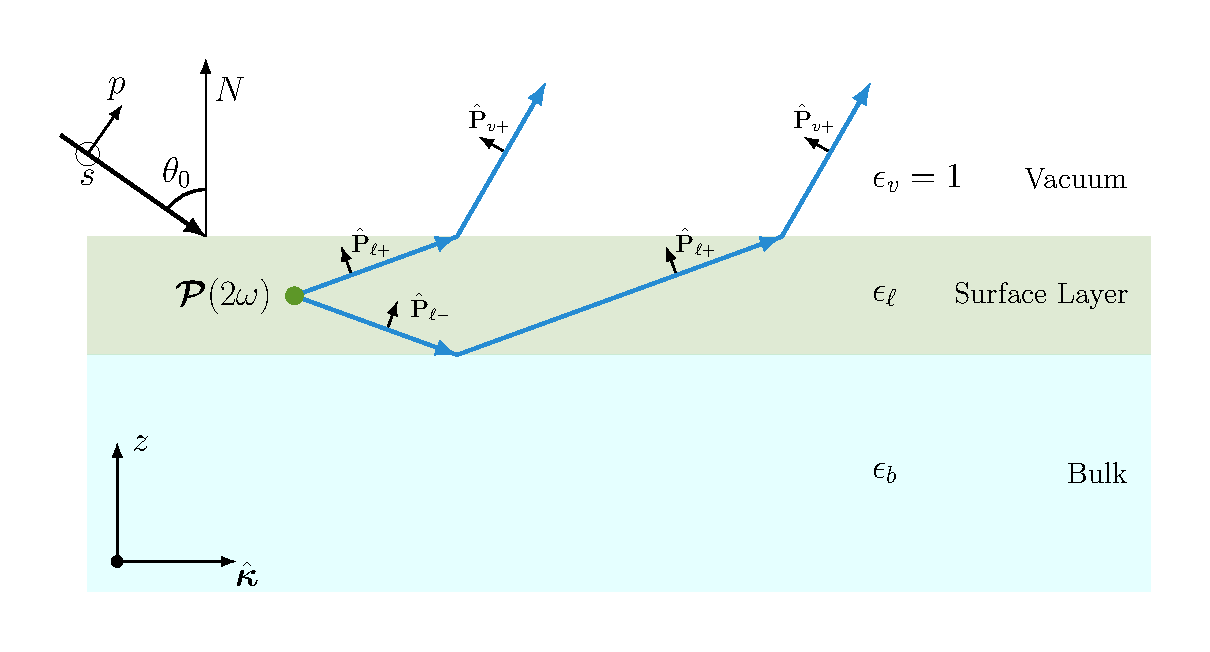
\includegraphics[width=0.5\textwidth]{content/figures/diag-3layer}
\caption{Sketch of the three layer model for SHG. Vacuum is on top with
$\epsilon_v=1$, the layer with nonlinear polarization 
$\boldsymbol{\mathcal{P}}(2\omega)$
is characterized with $\epsilon_{\ell}(\omega)$ and the bulk with
$\epsilon_{b}(\omega)$. In the dipolar approximation the bulk does not radiate
SHG. The thin arrows are along the direction of propagation, and the unit
vectors for $p$-polarization are denoted with thick arrows (capital letters
denote SH components). The unit vector for $s$-polarization points along $-y$
(out of the page).\label{fig:3layer}}
\end{figure}

To describe the propagation of the SH field, we see from Fig. \ref{fig:3layer},
that it is refracted at the layer-vacuum interface ($\ell v$), and  reflected
from the layer-bulk ($\ell b$) and layer-vacuum ($\ell v$) interfaces, thus we
define
\begin{equation}\label{r5}
\mathbf{T}^{\ell v}
= \hat{\mathbf{s}}T_{s}^{\ell v}\hat{\mathbf{s}} 
+ \hat{\mathbf{P}}_{v+}T_{p}^{\ell v}\hat{\mathbf{P}}_{\ell +},
\end{equation}
as the tensor for transmission from the $\ell v$ interface,
\begin{equation}\label{r6}
\mathbf{R}^{\ell b}
= \hat{\mathbf{s}}R_{s}^{\ell b}\hat{\mathbf{s}}
+ \hat{\mathbf{P}}_{\ell +}R_{p}^{\ell b}\hat{\mathbf{P}}_{\ell -},
\end{equation} 
as the tensor of reflection from the $\ell b$ interface, and
\begin{equation}\label{r6b}
\mathbf{R}^{\ell v}
= \hat{\mathbf{s}}R_{s}^{\ell v}\hat{\mathbf{s}}
+ \hat{\mathbf{P}}_{\ell -}R_{p}^{\ell v}\hat{\mathbf{P}}_{\ell +},
\end{equation} 
as that from the $\ell v$ interface. The Fresnel factors in uppercase letters,
$T^{ij}_{s,p}$ and $R^{ij}_{s,p}$, are evaluated at $2\omega$ from the following
well known formulas,\cite{ mizrahiJOSA88}
\begin{align}
t_s^{ij}(\omega) &=
\frac{2w_{i}(\omega)}{w_{i}(\omega)+w_{j}(\omega)},\\
t_{p}^{ij}(\omega) &=
\frac{2w_{i}(\omega)\sqrt{\epsilon_{i}(\omega)\epsilon_j(\omega)}}
     {w_{i}(\omega)\epsilon_{j}(\omega)+w_{j}(\omega)\epsilon_{i}(\omega)},\\
r_s^{ij}(\omega) &=
\frac{w_{i}(\omega) - w_{j}(\omega)}
     {w_{i}(\omega) + w_{j}(\omega)},\\
r_{p}^{ij}(\omega) &=
\frac{w_{i}(\omega)\epsilon_{j}(\omega) - w_{j}\epsilon_{i}(\omega)}
     {w_{i}(\omega)\epsilon_{j}(\omega) + w_{j}(\omega)\epsilon_{i}(\omega)}. 
\end{align}
From these expressions one can show that,
\begin{align}\label{mf}
1 + r^{\ell b}_{s} &= t^{\ell b}_{s}\nonumber\\
1 + r^{\ell b}_{p}
&= \frac{n_b}{n_\ell} 
t^{\ell b}_{p} 
\nonumber\\ 
1 - r^{\ell b}_{p}
&= \frac{n_\ell}{n_b}
   \frac{w_{b}}{w_{\ell}}t^{\ell b}_{p}\\ 
t^{\ell v}_{s,p} &= \frac{w_{\ell}}{w_{v}}t^{v\ell}_{s,p}\nonumber
.
\end{align}


%%%%%%%%%%%%%%%%%%%%%%%%%%%%%%%%%%%%%%%%%%%%%%%%%%%%%%%%%%%%%%%%%%%%%%%%%%%%%%%%
%%%%%%%%%%%%%%%%%%%%%%%%%%%%%%%%%%%%%%%%%%%%%%%%%%%%%%%%%%%%%%%%%%%%%%%%%%%%%%%%

\subsection{SSHG Yield}\label{sec:yield}

We obtain the total $2\omega$ radiated field by using Eqs. \eqref{r5},
\eqref{r6}, and \eqref{r6b},
\begin{equation*}\label{r7}
\mathbf{E}(2\omega)
= E_s(2\omega)
\left(
\mathbf{T}^{\ell v} + \mathbf{T}^{\ell v}\cdot\mathbf{R}^{\ell b}
\right)
\cdot\hat{\mathbf{s}}
+ E_{p+}(2\omega)\mathbf{T}^{\ell v}\cdot\hat{\mathbf{P}}_{\ell +}
 + E_{p-}(2\omega)\mathbf{T}^{\ell v}
\cdot\mathbf{R}^{\ell b}\cdot\hat{\mathbf{P}}_{\ell-}.
\end{equation*}
The first term is  the transmitted $s$-polarized field, the second one is the
reflected and then transmitted $s$-polarized field and the third and fourth
terms are the equivalent fields for $p$-polarization. The transmission is from
the layer into vacuum, and the reflection between the layer and the bulk. After
some simple algebra, we obtain
\begin{equation}\label{r8}
\mathbf{E}_{\ell}(2\omega) = \frac{\gamma i\tilde{\Omega}}{W_{\ell}}
\mathbf{H}_{\ell}\cdot\boldsymbol{\mathcal{P}}_\ell(2\omega),
\end{equation}
where,
\begin{equation}\label{r9}
\mathbf{H}_{\ell}
= \hat{\mathbf{s}}\,T_s^{\ell v}\left(1+R_s^{\ell b}\right)\hat{\mathbf{s}}
+ \hat{\mathbf{P}}_{v+}T_{p}^{\ell v}
\left(
\hat{\mathbf{P}}_{\ell +} +R_{p}^{\ell b}\hat{\mathbf{P}}_{\ell -}
\right). 
\end{equation}
The magnitude of the radiated SH field is given by
$E(2\omega)=\hat{\mathbf{e}}^{\mathrm{F}}\cdot\mathbf{E}_\ell(2\omega)$, where
$\hat{\mathbf{e}}^{\mathrm{F}}$ is the unit vector of the final polarization,
with $\mathrm{F}=S,P$, and then, $\hat{\mathbf{e}}^S=\hat{\mathbf{s}}$ and
$\hat{\mathbf{e}}^P=\hat{\mathbf{P}}_{v+}$. We expand the second term in
parenthesis of Eq. \eqref{r9} as
\begin{equation*}\label{m1}
\begin{split}
\hat{\mathbf{P}}_{\ell +} + R_{p}^{\ell b}\hat{\mathbf{P}}_{\ell -}
&= \frac{\sin\theta_{0}\hat{\mathbf{z}} - W_{\ell}\hat{\boldsymbol{\kappa}}}
        {N_{\ell}}
 + R_{p}^{\ell b}
   \frac{\sin\theta_{0}\hat{\mathbf{z}} + W_{\ell}\hat{\boldsymbol{\kappa}}}
        {N_{\ell}}
\\\nonumber
&= \frac{1}{N_{\ell}}
\left(
\sin\theta_{0}(1+R^{\ell b}_{p})\hat{\mathbf{z}}
- W_{\ell}(1-R^{\ell b}_{p})\hat{\boldsymbol{\kappa}} 
\right)
\\\nonumber 
&= \frac{T^{\ell b}_{p}}{N^{2}_{\ell}N_{b}}
\left(
  N^{2}_{b}\sin\theta_{0}\hat{\mathbf{z}} 
- N^{2}_{\ell}W_{b}\hat{\boldsymbol{\kappa}}
\right)
,
\end{split}
\end{equation*}
and rewrite Eq. \eqref{r8} as
\begin{equation}\label{r10}
E(2\omega) =
\frac{2\gamma i \omega}{cW_{\ell}}
\hat{\mathbf{e}}^{\mathrm{F}}
\cdot
\mathbf{H}_{\ell}
\cdot
\boldsymbol{\mathcal{P}}_\ell(2\omega) 
= \frac{2\gamma i \omega}{cW_{v}}
\mathbf{e}^{\,2\omega,\mathrm{F}}_{\ell}
\cdot\boldsymbol{\mathcal{P}}_\ell(2\omega),
\end{equation}
where
\begin{equation}\label{r12mm}
\mathbf{e}^{2\omega,\mathrm{F}}_{\ell} =
\hat{\mathbf{e}}^{\mathrm{F}}\cdot 
\Bigg[
\hat{\mathbf{s}}T_{s}^{v\ell}T_{s}^{\ell b}\hat{\mathbf{s}} + 
\hat{\mathbf{P}}_{v+}
\frac{T^{v\ell}_{p}T^{\ell b}_{p}}
     {N^{2}_{\ell}N_{b}}
\left(
  N^{2}_{b}\sin\theta_{0}\hat{\mathbf{z}}
- N^{2}_{\ell}W_{b}\hat{\boldsymbol{\kappa}}
\right)
\Bigg].
\end{equation}

In the three layer model the nonlinear polarization is located in layer
$\ell$, thus, we evaluate the fundamental field required in Eq. \eqref{tres}
in this layer as well. We write
\begin{equation}\label{m2}
\begin{split}
\mathbf{E}_{\ell}(\omega)=E_0\left(
\hat{\mathbf{s}} t^{v\ell}_s(1+r^{\ell b}_s)\hat{\mathbf{s}}
+
\hat{\mathbf{p}}_{\ell-}
 t^{v\ell}_{p}
\hat{\mathbf{p}}_{v-}
+
\hat{\mathbf{p}}_{\ell+}
t^{v\ell}_{p}r^{\ell b}_{p}
\hat{\mathbf{p}}_{v-}
\right)\cdot\hat{\mathbf{e}}^{\mathrm{in}}=E_0\mathbf{e}^\omega_{\ell}
,
\end{split}
\end{equation} 
and following the steps that lead to Eq. \eqref{r12mm}, we find that
\begin{equation}\label{m12}
\mathbf{e}^{\omega,\mathrm{i}}_{\ell}
= \left[
\hat{\mathbf{s}}t_{s}^{v\ell}t_{s}^{\ell b}\hat{\mathbf{s}} 
+ \frac{t^{v\ell}_{p}t^{\ell b}_{p}}
       {n^{2}_{\ell}n_{b}}
\left(
  n^{2}_{b}\sin\theta_{0}\hat{\mathbf{z}}
+ n^{2}_{\ell}w_{b}\hat{\boldsymbol{\kappa}}
\right)
\hat{\mathbf{p}}_{v-}
\right]
\cdot\hat{\mathbf{e}}^{\mathrm{i}}.
\end{equation}

We pause here to reduce this result to the case where the nonlinear polarization
$\mathbf{P}(2\omega)$ radiates from vacuum instead from the layer $\ell$. For
such case we simply take $\epsilon_{\ell}(2\omega) = 1$ and $\ell = v$ ($T^{\ell
v}_{s,p} = 1$), to get
\begin{equation}\label{eq:r13}
\mathbf{e}^{\,2\omega}_{v} = \hat{\mathbf{e}}^{\mathrm{F}}\cdot
\left[
\hat{\mathbf{s}}T_{s}^{v b}\hat{\mathbf{s}} + \hat{\mathbf{P}}_{v+}
\frac{T^{v b}_{p}}{\sqrt{\epsilon_{b}(2\omega)}}
\left(
  \epsilon_{b}(2\omega)\sin\theta_{0}\hat{\mathbf{z}}
- W_{b}\hat{\boldsymbol{\kappa}}
\right) 
\right],
\end{equation}
which agrees with Eq. (3.10) of Ref. \cite{mizrahiJOSA88}.

In the 3-layer model the SH polarization $\boldsymbol{\mathcal{P}}(2\omega)$ is
located in layer $\ell$, where we evaluate the fundamental field required in Eq.
\eqref{eq:tres}. We write
\begin{equation}\label{eq:m2}
\begin{split}
\mathbf{E}_{\ell}(\omega) 
&= E_{0}
\left(
  \hat{\mathbf{s}} t^{v\ell}_{s}(1+r^{\ell b}_{s})\hat{\mathbf{s}}
+ \hat{\mathbf{p}}_{\ell-}t^{v\ell}_{p}\hat{\mathbf{p}}_{v-}
+ \hat{\mathbf{p}}_{\ell+}t^{v\ell}_{p}r^{\ell b}_{p}\hat{\mathbf{p}}_{v-}
\right)
\cdot\hat{\mathbf{e}}^{\mathrm{i}}\\
&= E_{0}\mathbf{e}^\omega_{\ell},
\end{split}
\end{equation} 
where $\hat{\mathbf{e}}^{\mathrm{i}}$ is the $s$ ($\hat{\mathbf{s}}$) or $p$
($\hat{\mathbf{p}}_{v-}$) incoming polarization of the fundamental electric
field. This field is composed of the transmitted field and its first reflection
from the $\ell b$ interface for $s$ and $p$ polarizations. The fundamental
field, once inside the layer $\ell$ will be reflected multiple times at the
$\ell v$ and $\ell b$ interfaces. However, each reflection will diminish the
intensity of the fundamental field. As the SSHG yield scales with the square of
this field, the contribution of the subsequent reflections after the one
considered in Eq. \eqref{eq:m2} can be safely neglected. From Eq. \eqref{eq:mf}
we find that
\begin{equation}\label{eq:m12}
\mathbf{e}^{\omega}_{\ell} =
\left[
  \hat{\mathbf{s}}t_{s}^{v\ell}t_{s}^{\ell b}\hat{\mathbf{s}} 
+ \frac{t^{v\ell}_{p}t^{\ell b}_{p}}{n^{2}_{\ell} n_{b}}
\left(
  n^{2}_{b}\sin\theta_{0}\hat{\mathbf{z}} 
+ n^{2}_{\ell} w_b\hat{\boldsymbol{\kappa}}
\right)
\hat{\mathbf{p}}_{v-}
\right]
\cdot\hat{\mathbf{e}}^{\mathrm{in}}.  
\end{equation}  
To connect with the work in Ref. \cite{mizrahiJOSA88}, we evaluate the fields in
the bulk instead of the layer $\ell$and simply take $n_{\ell} = n_{b}$
$(t^{\ell b}_{s,p} = 1)$, to obtain
\begin{equation}\label{eq:m13}
\mathbf{e}^{\omega}_{b} =
\left[
  \hat{\mathbf{s}}t_{s}^{vb}\hat{\mathbf{s}}
+ \frac{t^{vb}_{p}}{n_{b}}
\left(\sin\theta_{0}\hat{\mathbf{z}} + w_b\hat{\boldsymbol{\kappa}}\right) 
\hat{\mathbf{p}}_{v-}
\right]
\cdot\hat{\mathbf{e}}^{\mathrm{in}},  
\end{equation} 
that is in agreement with Eq. (3.5) of Ref. \cite{mizrahiJOSA88}.

Replacing $\mathbf{E}(\omega)\to E_0\mathbf{e}^{\omega,\mathrm{i}}_\ell$,  
in Eq. \eqref{tres}, we obtain that
\begin{equation}\label{m4}
\boldsymbol{\mathcal{P}}_\ell(2\omega) = 
\left\{
\begin{array}{cc}  
E^{2}_{0}\,\boldsymbol{\chi}:
\mathbf{e}^{\omega,\mathrm{i}}_{\ell}\mathbf{e}^{\omega,\mathrm{i}}_{\ell}
& \text{(cgs units)} \\\\
\epsilon_{0}E^{2}_{0}\,\boldsymbol{\chi}:
\mathbf{e}^{\omega,\mathrm{i}}_{\ell}\mathbf{e}^{\omega,\mathrm{i}}_{\ell}
& \text{(MKS units)} \\
\end{array}
\right.,
\end{equation}
where $\mathbf{e}^{\omega,\mathrm{i}}_{\ell}$ is given by Eq. \eqref{m12},
and thus
Eq. \eqref{r10} reduces to ($W_{v}=\cos\theta_{0}$)
\begin{equation}\label{mr10}
E(2\omega) =
\frac{2\eta i \omega}{c\cos\theta_{0}}
\mathbf{e}^{2\omega,\mathrm{F}}_{\ell}\cdot\boldsymbol{\chi}:
\mathbf{e}^{\omega,\mathrm{i}}_{\ell}\mathbf{e}^{\omega,\mathrm{i}}_{\ell}
,
\end{equation}
where $\eta=2\pi$ for cgs units and $\eta=1/2$ for MKS units. For ease of
notation, we define
\begin{equation}\label{mc0}
\Upsilon_{\mathrm{iF}}
\equiv 
\mathbf{e}^{2\omega,\mathrm{F}}_{\ell}\cdot\boldsymbol{\chi}:
\mathbf{e}^{\omega,\mathrm{i}}_{\ell}\mathbf{e}^{\omega,\mathrm{i}}_{\ell}
.
\end{equation}
From Eqs. \eqref{uno},
\eqref{dos}, and \eqref{mr10} we obtain that
\begin{equation}\label{mc6}
\mathcal{R}_{\mathrm{iF}}
=\frac{\eta\omega^{2}}{c^{3}\cos^{2}\theta_{0}}
\left\vert  
\frac{1}{n_{\ell}}
\Upsilon_{\mathrm{iF}}
\right\vert^{2},
\end{equation}
as the SSHG yield, where $\eta =32\pi^3$ for cgs units and
$\eta=1/(2\epsilon_0)$ in MKS units. Since $\boldsymbol{\chi}$ is a surface
second order nonlinear susceptibility, in the MKS unit system is given in
$\mathrm{m}^{2}/\mathrm{V}$, and thus $\mathcal{R}_{\mathrm{iF}}$ is given in
$\mathrm{m}^{2}/\mathrm{W}$.

It is worth mentioning that we can easily recover the results from Ref.
\cite{mizrahiJOSA88}, which are in turn equivalent to those in Ref.
\cite{sipePRB87}. We simply take
$\mathbf{e}^{2\omega}_{\ell}\to\mathbf{e}^{2\omega}_{v}$,
$\mathbf{e}^{\omega}_{\ell}\to\mathbf{e}^{\omega}_{b}$, and we have
\begin{equation}\label{eq:m69}
\mathcal{R}_{\mathrm{iF}}(2\omega) =
\frac{\eta\omega^{2}}{c^{3}\cos^{2}\theta_{0}}
\left\vert\mathbf{e}^{\,2\omega}_{v}\cdot
\boldsymbol{\chi}:\mathbf{e}^{\omega}_{b}\mathbf{e}^{\omega}_{b}
\right\vert^{2}.
\end{equation}
This is the SSHG yield  of a nonlinear polarization sheet radiating from the
vacuum region above the surface, with the fundamental field evaluated below the
surface in the bulk of the material characterized by $\epsilon_{b}(\omega)$.


%%%%%%%%%%%%%%%%%%%%%%%%%%%%%%%%%%%%%%%%%%%%%%%%%%%%%%%%%%%%%%%%%%%%%%%%%%%%%%%%
%%%%%%%%%%%%%%%%%%%%%%%%%%%%%%%%%%%%%%%%%%%%%%%%%%%%%%%%%%%%%%%%%%%%%%%%%%%%%%%%

\section{Some limiting cases of interest}\label{app:limiting_cases}

In this section, we derive the expresions for $\mathcal{R}_{pP}$ for different
limiting cases. We evaluate $\mathcal{P}(2\omega)$ and the fundamental fields in
different regions. It is worth noting that the first case, the three layer
model, can be reduced to any of the other cases by simply considering where we
want to evaluate the $1\omega$ and $2\omega$ terms.


\subsection{The two layer model}

In order to reduce above result to that of Ref. \cite{mizrahiJOSA88} and
\cite{sipePRB87}, we now consider that $\mathcal{P}(2\omega)$ is evaluated in
the vacuum region, while the fundamental fields are evaluated in the bulk
region. To do this, we take the $2\omega$ radiations factors for vacuum by
taking $\ell=v$, thus $\epsilon_{\ell}(2\omega)=1$, $T^{\ell v}_{p}=1$, $T^{\ell
b}_{p}=T^{vb}_{p}$, and the fundamental field inside medium $b$ by taking
$\ell=b$, thus $\epsilon_{\ell}(\omega)=\epsilon_{b}(\omega)$,
$t^{v\ell}_{p}=t^{vb}_{p}$, and $t^{\ell b}_{p}=1$. With these choices
\begin{equation*}\label{m800}
\mathbf{e}^{\,2\omega}_{v}\cdot\boldsymbol{\chi}:
\mathbf{e}^\omega_{b}\mathbf{e}^\omega_{b}
\equiv\Gamma^{vb}_{pP}\,r^{vb}_{pP}
,
\end{equation*}
where,
\begin{equation*}\label{m82}
\begin{split}
r^{vb}_{pP}
&= \epsilon_{b}(2\omega)\sin\theta_{0}
\Big(
\sin^2\theta_{0}\chi_{zzz} + k^{2}_{b}\chi_{zxx}
\Big)\\
&- k_{b}K_{b}
\Big(
2\sin\theta_{0}\chi_{xxz} + k_{b}\chi_{xxx}\cos(3\phi) 
\Big) 
,
\end{split}
\end{equation*}
and 
\begin{equation*}\label{m78}
\Gamma^{vb}_{pP}
= \frac{T^{v b}_{p}(t^{vb}_{p})^2}
       {\epsilon_{b}(\omega)\sqrt{\epsilon_{b}(2\omega)}}.
\end{equation*}


\subsection{Taking \texorpdfstring{$\mathcal{P}(2\omega)$}{P(2w)} and the
fundamental fields in the bulk}

To consider the $2\omega$ fields in the bulk, we start with Eq. \eqref{r9} but
substitute $\ell\rightarrow b$, thus
\begin{equation*}
\mathbf{H}_{b}
= \hat{\mathbf{s}}\,T_s^{b v}\left(1+R_{s}^{b b}\right)\hat{\mathbf{s}}
+ \hat{\mathbf{P}}_{v+}T_{p}^{b v}
\left(
\hat{\mathbf{P}}_{b+} + R_{p}^{b b}\hat{\mathbf{P}}_{b-}
\right).
\end{equation*}
$R_{p}^{b b}$ and $R_{s}^{b b}$ are zero, so we are left with
\begin{equation*}
\begin{split}
\mathbf{H}_{b}
&= \hat{\mathbf{s}}\,T_s^{b v}\hat{\mathbf{s}}
 + \hat{\mathbf{P}}_{v+}T_{p}^{b v}\hat{\mathbf{P}}_{b+}\\
&= \frac{K_{b}}{K_{v}}\left(\hat{\mathbf{s}}\,T_s^{vb}\hat{\mathbf{s}}
 + \hat{\mathbf{P}}_{v+}T_{p}^{vb}\hat{\mathbf{P}}_{b+}\right)\\
&= \frac{K_{b}}{K_{v}}
   \left[
   \hat{\mathbf{s}}\,T_s^{vb}\hat{\mathbf{s}}
 + \hat{\mathbf{P}}_{v+}
   \frac{T_{p}^{vb}}{\sqrt{\epsilon_{b}(2\omega)}}
   (\sin\theta_{0}\hat{\mathbf{z}}
 - K_{b}\cos\phi\hat{\mathbf{x}} 
 - K_{b}\sin\phi\hat{\mathbf{y}})
   \right],
\end{split}
\end{equation*}
and we define
\begin{equation*}
\mathbf{e}^{\,2\omega}_{b}
= \frac{K_{b}}{K_{v}}\,\hat{\mathbf{e}}^{\mathrm{out}}\cdot
\left[
   \hat{\mathbf{s}}\,T_s^{vb}\hat{\mathbf{s}}
 + \hat{\mathbf{P}}_{v+}
   \frac{T_{p}^{vb}}{\sqrt{\epsilon_{b}(2\omega)}}
   (\sin\theta_{0}\hat{\mathbf{z}}
 - K_{b}\cos\phi\hat{\mathbf{x}} 
 - K_{b}\sin\phi\hat{\mathbf{y}})
   \right].
\end{equation*}
For $\mathcal{R}_{pP}$, we require
$\hat{\mathbf{e}}^{\mathrm{out}}=\hat{\mathbf{P}}_{v+}$, so we have that
\begin{equation*}
\mathbf{e}^{\,2\omega}_{b}
= \frac{K_{b}}{K_{v}}
  \frac{T_{p}^{vb}}{\sqrt{\epsilon_{b}(2\omega)}}
  (\sin\theta_{0}\hat{\mathbf{z}}
- K_{b}\cos\phi\hat{\mathbf{x}} 
- K_{b}\sin\phi\hat{\mathbf{y}}).
\end{equation*}

The $1\omega$ fields will still be evaluated inside the bulk, so we have
\begin{equation*}
\mathbf{e}^{\omega}_{b}
= \left[
\hat{\mathbf{s}}t_{s}^{vb}\hat{\mathbf{s}}
+ \frac{t^{vb}_{p}}{\sqrt{\epsilon_{b}(\omega)}}
\left(
  \sin\theta_{0}\hat{\mathbf{z}}
+ k_{b}\cos\phi\hat{\mathbf{x}}
+ k_{b}\sin\phi\hat{\mathbf{y}}
\right) 
\hat{\mathbf{p}}_{v-}
\right]
\cdot\hat{\mathbf{e}}^{\mathrm{in}},  
\end{equation*}
and for our particular case of
$\hat{\mathbf{e}}^{\mathrm{in}}=\hat{\mathbf{p}}_{v-}$,
\begin{equation*}
\mathbf{e}^{\omega}_{b}
= \frac{t^{vb}_{p}}{\sqrt{\epsilon_{b}(\omega)}}
\left(
  \sin\theta_{0}\hat{\mathbf{z}}
+ k_{b}\cos\phi\hat{\mathbf{x}}
+ k_{b}\sin\phi\hat{\mathbf{y}}
\right),
\end{equation*}
and
\begin{equation*}
\begin{split}
\mathbf{e}^{\omega}_{b}\mathbf{e}^{\omega}_{b}
&= \frac{\left(t^{vb}_{p}\right)^{2}}{\epsilon_{b}(\omega)}
\left(
  \sin\theta_{0}\hat{\mathbf{z}}
+ k_{b}\cos\phi\hat{\mathbf{x}}
+ k_{b}\sin\phi\hat{\mathbf{y}}
\right)^{2}\\
&= \frac{\left(t^{vb}_{p}\right)^{2}}{\epsilon_{b}(\omega)}
\big(
  \sin^{2}\theta_{0}\hat{\mathbf{z}}\hat{\mathbf{z}}
+ k^{2}_{b}\cos^{2}\phi\hat{\mathbf{x}}\hat{\mathbf{x}}
+ k^{2}_{b}\sin^{2}\phi\hat{\mathbf{y}}\hat{\mathbf{y}}\\
&\qquad\qquad
+ 2k_{b}\sin\theta_{0}\cos\phi\hat{\mathbf{z}}\hat{\mathbf{x}}
+ 2k_{b}\sin\theta_{0}\sin\phi\hat{\mathbf{z}}\hat{\mathbf{y}}
+ 2k^{2}_{b}\sin\phi\cos\phi\hat{\mathbf{x}}\hat{\mathbf{y}}
\big)
\end{split}
\end{equation*}

So lastly, we have that
\begin{equation*}
\begin{split}
\mathbf{e}^{\,2\omega}_{b}\cdot
\boldsymbol{\chi}:\mathbf{e}^{\omega}_{b}\mathbf{e}^{\omega}_{b} =
\frac{K_{b}}{K_{v}}
\frac{T_{p}^{vb}\left(t^{vb}_{p}\right)^{2}}
     {\epsilon_{b}(\omega)\sqrt{\epsilon_{b}(2\omega)}}
&\big(
   \sin^{3}\theta_{0}\chi_{zzz}\\
&+ k^{2}_{b}\sin\theta_{0}\cos^{2}\phi\chi_{zxx}\\
&+ k^{2}_{b}\sin\theta_{0}\sin^{2}\phi\chi_{zyy}\\
&+ 2k_{b}\sin^{2}\theta_{0}\cos\phi\chi_{zzx}\\
&+ 2k_{b}\sin^{2}\theta_{0}\sin\phi\chi_{zzy}\\
&+ 2k^{2}_{b}\sin\theta_{0}\sin\phi\cos\phi\chi_{zxy}\\
&- K_{b}\sin^{2}\theta_{0}\cos\phi\chi_{xzz}\\
&- k^{2}_{b}K_{b}\cos^{3}\phi\chi_{xxx}\\
&- k^{2}_{b}K_{b}\sin^{2}\phi\cos\phi\chi_{xyy}\\
&- 2k_{b}K_{b}\sin\theta_{0}\cos^{2}\phi\chi_{xzx}\\
&- 2k_{b}K_{b}\sin\theta_{0}\sin\phi\cos\phi\chi_{xzy}\\
&- 2k^{2}_{b}K_{b}\sin\phi\cos^{2}\phi\chi_{xxy}\\
&- K_{b}\sin^{2}\theta_{0}\sin\phi\chi_{yzz}\\
&- k^{2}_{b}K_{b}\sin\phi\cos^{2}\phi\chi_{yxx}\\
&- k^{2}_{b}K_{b}\sin^{3}\phi\chi_{yyy}\\
&- 2k_{b}K_{b}\sin\theta_{0}\sin\phi\cos\phi\chi_{yzx}\\
&- 2k_{b}K_{b}\sin\theta_{0}\sin^{2}\phi\chi_{yzy}\\
&- 2k^{2}_{b}K_{b}\sin^{2}\phi\cos\phi\chi_{yxy}
\big),
\end{split}
\end{equation*}
and we can eliminate many terms since
$\chi_{zzx}=\chi_{zzy}=\chi_{zxy}=\chi_{xzz}=\chi_{xzy}=\chi_{xxy}=\chi_{yzz}
=\chi_{yxx}=\chi_{yyy}=\chi_{yzx}=0$, and substituting the equivalent
components of $\boldsymbol{\chi},$
\begin{equation*}
\begin{split}
=
\frac{K_{b}}{K_{v}}
\Gamma^{b}_{pP}
&\big(
   \sin^{3}\theta_{0}\chi_{zzz}\\
&+ k^{2}_{b}\sin\theta_{0}\cos^{2}\phi\chi_{zxx}\\
&+ k^{2}_{b}\sin\theta_{0}\sin^{2}\phi\chi_{zxx}\\
&- 2k_{b}K_{b}\sin\theta_{0}\cos^{2}\phi\chi_{xxz}\\
&- 2k_{b}K_{b}\sin\theta_{0}\sin^{2}\phi\chi_{xxz}\\
&- k^{2}_{b}K_{b}\cos^{3}\phi\chi_{xxx}\\
&+ k^{2}_{b}K_{b}\sin^{2}\phi\cos\phi\chi_{xxx}\\
&+ 2k^{2}_{b}K_{b}\sin^{2}\phi\cos\phi\chi_{xxx}
\big),
\end{split}
\end{equation*}
and reducing,
\begin{equation*}
\begin{split}
=
\frac{K_{b}}{K_{v}}
\Gamma^{b}_{pP}
&\big(
   \sin^{3}\theta_{0}\chi_{zzz}\\
&+ k^{2}_{b}\sin\theta_{0}(\sin^{2}\phi + \cos^{2}\phi)\chi_{zxx}\\
&- 2k_{b}K_{b}\sin\theta_{0}(\sin^{2}\phi + \cos^{2}\phi)\chi_{xxz}\\
&+ k^{2}_{b}K_{b}(3\sin^{2}\phi\cos\phi - \cos^{3}\phi)\chi_{xxx}
\big)\\\\
=
\frac{K_{b}}{K_{v}}
\Gamma^{b}_{pP}
&\big(
  \sin^{3}\theta_{0}\chi_{zzz} 
+ k^{2}_{b}\sin\theta_{0}\chi_{zxx}
- 2k_{b}K_{b}\sin\theta_{0}\chi_{xxz}
- k^{2}_{b}K_{b}\chi_{xxx}\cos3\phi
\big),
\end{split}
\end{equation*}
where,
\begin{equation*}
\Gamma^{b}_{pP} =
\frac{T_{p}^{vb}\left(t^{vb}_{p}\right)^{2}}
     {\epsilon_{b}(\omega)\sqrt{\epsilon_{b}(2\omega)}}.
\end{equation*}

We find the equivalent expression for $\mathcal{R}$ evaluated inside the bulk
as
\begin{equation*}
R(2\omega) =
\frac{32\pi^{3} \omega^{2}}{c^{3}K^{2}_{b}}
\left\vert
\mathbf{e}^{\,2\omega}_{b}\cdot\boldsymbol{\chi}:
\mathbf{e}^{\omega}_{b}\mathbf{e}^{\omega}_{b}
\right\vert^{2} 
,
\end{equation*}
and we can remove the $K_{b}/K_{v}$ factor completely and reduce to the
standard form of
\begin{equation*}
R(2\omega) =
\frac{32\pi^{3} \omega^{2}}{c^{3}\cos^{2}\theta_{0}}
\left\vert
\mathbf{e}^{\,2\omega}_{b}\cdot\boldsymbol{\chi}:
\mathbf{e}^{\omega}_{b}\mathbf{e}^{\omega}_{b}
\right\vert^{2}.
\end{equation*}


\subsection{Taking \texorpdfstring{$\mathcal{P}(2\omega)$}{P(2w)} and the
fundamental fields in the vacuum}

To consider the $1\omega$ fields in the vacuum, we start with Eq. \eqref{m2}
but substitute $\ell\rightarrow v$, thus
\begin{equation*}
\mathbf{E}_{v}(\omega)= E_{0}
\left[
  \hat{\mathbf{s}} t^{vv}_s(1+r^{v b}_s)\hat{\mathbf{s}}
+ \hat{\mathbf{p}}_{v-}t^{vv}_{p}\hat{\mathbf{p}}_{v-}
+ \hat{\mathbf{p}}_{v+}t^{vv}_{p}r^{v b}_{p}\hat{\mathbf{p}}_{v-}
\right]
\cdot\hat{\mathbf{e}}^{\mathrm{in}}
,
\end{equation*}
$t_{p}^{vv}$ and $t_{s}^{vv}$ are one, so we are left with
\begin{equation*}
\begin{split}
\mathbf{e}^{\omega}_{v}
&= \left[
  \hat{\mathbf{s}}(1+r^{v b}_s)\hat{\mathbf{s}}
+ \hat{\mathbf{p}}_{v-}\hat{\mathbf{p}}_{v-}
+ \hat{\mathbf{p}}_{v+}r^{v b}_{p}\hat{\mathbf{p}}_{v-}
\right]
\cdot\hat{\mathbf{e}}^{\mathrm{in}}\\
&= \left[
  \hat{\mathbf{s}}(t^{vb}_s)\hat{\mathbf{s}}
+ (\hat{\mathbf{p}}_{v-} + \hat{\mathbf{p}}_{v+}r^{v b}_{p})
  \hat{\mathbf{p}}_{v-}
\right]
\cdot\hat{\mathbf{e}}^{\mathrm{in}}\\
&= \left[
  \hat{\mathbf{s}}(t^{vb}_s)\hat{\mathbf{s}}
+ \frac{1}{\sqrt{\epsilon_{v}(\omega)}}
\big(
  k_{v}(1 - r^{vb}_{p})\hat{\boldsymbol{\kappa}}
+ \sin\theta_{0}(1 + r^{vb}_{p})
\hat{\mathbf{z}}
\big)
  \hat{\mathbf{p}}_{v-}
\right]\\
&= \left[
  \hat{\mathbf{s}}(t^{vb}_s)\hat{\mathbf{s}}
+ \left(
  \frac{k_{b}}{\sqrt{\epsilon_{b}(\omega)}}
  t^{v b}_{p}\hat{\boldsymbol{\kappa}} 
+ \sqrt{\epsilon_{b}(\omega)}\sin\theta_{0}
  t^{v b}_{p}\hat{\mathbf{z}}
  \right)
  \hat{\mathbf{p}}_{v-}
\right]
\cdot\hat{\mathbf{e}}^{\mathrm{in}}\\
&= \left[
  \hat{\mathbf{s}}(t^{vb}_s)\hat{\mathbf{s}}
+ \frac{t^{v b}_{p}}{\sqrt{\epsilon_{b}(\omega)}}\left(
  k_{b}\cos\phi\hat{\mathbf{x}}
+ k_{b}\sin\phi\hat{\mathbf{y}}
+ \epsilon_{b}(\omega)\sin\theta_{0}\hat{\mathbf{z}}
  \right)
  \hat{\mathbf{p}}_{v-}
\right]
\cdot\hat{\mathbf{e}}^{\mathrm{in}}.
\end{split}
\end{equation*}
For $\mathcal{R}_{pP}$ we require that $\hat{\mathbf{e}}^{\mathrm{in}} =
\hat{\mathbf{p}}_{v-}$, so
\begin{equation*}
\mathbf{e}^{\omega}_{v} =
\frac{t^{v b}_{p}}{\sqrt{\epsilon_{b}(\omega)}}
\left(
  k_{b}\cos\phi\hat{\mathbf{x}}
+ k_{b}\sin\phi\hat{\mathbf{y}}
+ \epsilon_{b}(\omega)\sin\theta_{0}\hat{\mathbf{z}}
  \right),
\end{equation*}
and
\begin{equation*}
\begin{split}
\mathbf{e}^{\omega}_{v}\mathbf{e}^{\omega}_{v} =
\left(\frac{t^{v b}_{p}}{\sqrt{\epsilon_{b}(\omega)}}\right)^{2}
&\big[
   k^{2}_{b}\cos^{2}\phi\hat{\mathbf{x}}\hat{\mathbf{x}}\\
&+ k^{2}_{b}\sin^{2}\phi\hat{\mathbf{y}}\hat{\mathbf{y}}\\
&+ \epsilon^{2}_{b}(\omega)\sin^{2}\theta_{0}
   \hat{\mathbf{z}}\hat{\mathbf{z}}\\
&+ 2k^{2}_{b}\sin\phi\cos\phi\hat{\mathbf{x}}\hat{\mathbf{y}}\\
&+ 2\epsilon_{b}(\omega)k_{b}\sin\theta_{0}\sin\phi
   \hat{\mathbf{y}}\hat{\mathbf{z}}\\
&+ 2\epsilon_{b}(\omega)k_{b}\sin\theta_{0}\cos\phi
   \hat{\mathbf{x}}\hat{\mathbf{z}}
\big].
\end{split}
\end{equation*}

We also require the $2\omega$ fields evaluated in the vacuum, so
\begin{equation}
\mathbf{e}^{\,2\omega}_{v} = \hat{\mathbf{e}}^{\mathrm{out}}
\cdot\left[
\hat{\mathbf{s}}T_s^{v b}\hat{\mathbf{s}} + \hat{\mathbf{P}}_{v+}
\frac{T^{v b}_{p}}{\sqrt{\epsilon_{b}(2\omega)}}
\left(
  \epsilon_{b}(2\omega)\sin\theta_{0}\hat{\mathbf{z}}
  - K_{b}\hat{\boldsymbol{\kappa}}
\right) 
\right],
\end{equation}
and with $\hat{\mathbf{e}}^{\mathrm{out}} = \hat{\mathbf{P}}_{v+}$ we have
\begin{equation}
\mathbf{e}^{\,2\omega}_{v} =
\frac{T^{v b}_{p}}{\sqrt{\epsilon_{b}(2\omega)}}
\left(
\epsilon_{b}(2\omega)\sin\theta_{0}\hat{\mathbf{z}}
- K_{b}\cos\phi\hat{\mathbf{x}}
- K_{b}\sin\phi\hat{\mathbf{y}}
\right).
\end{equation}

So lastly, we have that
\begin{equation*}
\begin{split}
\mathbf{e}^{\,2\omega}_{v}\cdot
\boldsymbol{\chi}:\mathbf{e}^{\omega}_{v}\mathbf{e}^{\omega}_{v}
=\qquad\qquad&\\
\frac{T^{v b}_{p}}{\sqrt{\epsilon_{b}(2\omega)}}
\left(\frac{t^{v b}_{p}}{\sqrt{\epsilon_{b}(\omega)}}\right)^{2}
&\big[
    \epsilon_{b}(2\omega)k^{2}_{b}
    \sin\theta_{0}\cos^{2}\phi\chi_{zxx}\\
&+  \epsilon_{b}(2\omega)k^{2}_{b}
    \sin\theta_{0}\sin^{2}\phi\chi_{zyy}\\
&+  \epsilon^{2}_{b}(\omega)\epsilon_{b}(2\omega)
    \sin^{3}\theta_{0}\chi_{zzz}\\
&+ 2\epsilon_{b}(2\omega)k^{2}_{b}\sin\theta_{0}
    \sin\phi\cos\phi\chi_{zxy}\\
&+ 2\epsilon_{b}(\omega)\epsilon_{b}(2\omega)k_{b}
    \sin^{2}\theta_{0}\sin\phi\chi_{zyz}\\
&+ 2\epsilon_{b}(\omega)\epsilon_{b}(2\omega)k_{b}
    \sin^{2}\theta_{0}\cos\phi\chi_{zxz}\\
&-  k^{2}_{b}K_{b}\cos^{3}\phi\chi_{xxx}\\
&-  k^{2}_{b}K_{b}\sin^{2}\phi\cos\phi\chi_{xyy}\\
&-  \epsilon^{2}_{b}(\omega)K_{b}
    \sin^{2}\theta_{0}\cos\phi\chi_{xzz}\\
&- 2k^{2}_{b}K_{b}\sin\phi\cos^{2}\phi\chi_{xxy}\\
&- 2\epsilon_{b}(\omega)k_{b}K_{b}
    \sin\theta_{0}\sin\phi\cos\phi\chi_{xyz}\\
&- 2\epsilon_{b}(\omega)k_{b}K_{b}
    \sin\theta_{0}\cos^{2}\phi\chi_{xxz}\\
&-  k^{2}_{b}K_{b}\sin\phi\cos^{2}\phi\chi_{yxx}\\
&-  k^{2}_{b}K_{b}\sin^{3}\phi\chi{yyy}\\
&-  \epsilon^{2}_{b}(\omega)K_{b}
    \sin^{2}\theta_{0}\sin\phi\chi_{yzz}\\
&- 2k^{2}_{b}K_{b}\sin^{2}\phi\cos\phi\chi_{yxy}\\
&- 2\epsilon_{b}(\omega)k_{b}K_{b}
    \sin\theta_{0}\sin^{2}\phi\chi_{yyz}\\
&- 2\epsilon_{b}(\omega)k_{b}K_{b}
    \sin\theta_{0}\sin\phi\cos\phi\chi_{yxz}
\big],
\end{split}
\end{equation*}
and after eliminating components,
\begin{equation*}
\begin{split}
= \Gamma^{v}_{pP}&\big[
    \epsilon^{2}_{b}(\omega)\epsilon_{b}
    (2\omega)\sin^{3}\theta_{0}\chi_{zzz}\\
&+  \epsilon_{b}(2\omega)k^{2}_{b}
    \sin\theta_{0}\cos^{2}\phi\chi_{zxx}\\
&+  \epsilon_{b}(2\omega)k^{2}_{b}
    \sin\theta_{0}\sin^{2}\phi\chi_{zxx}\\
&- 2\epsilon_{b}(\omega)k_{b}K_{b}
    \sin\theta_{0}\cos^{2}\phi\chi_{xxz}\\
&- 2\epsilon_{b}(\omega)k_{b}K_{b}
    \sin\theta_{0}\sin^{2}\phi\chi_{xxz}\\
&+ 3k^{2}_{b}K_{b}\sin^{2}\phi\cos\phi\chi_{xxx}\\
&-  k^{2}_{b}K_{b}\cos^{3}\phi\chi_{xxx}
\big]\\\\
= \Gamma^{v}_{pP}&\big[
    \epsilon^{2}_{b}(\omega)\epsilon_{b}(2\omega)
    \sin^{3}\theta_{0}\chi_{zzz}
 +  \epsilon_{b}(2\omega)k^{2}_{b}\sin\theta_{0}\chi_{zxx}\\
&- 2\epsilon_{b}(\omega)k_{b}K_{b}\sin\theta_{0}\chi_{xxz}
 -  k^{2}_{b}K_{b}\chi_{xxx}\cos3\phi
\big],
\end{split}
\end{equation*}
where
\begin{equation*}
\Gamma^{v}_{pP} =
\frac{T^{v b}_{p}\left(t^{v b}_{p}\right)^{2}}
     {\epsilon_{b}(\omega)\sqrt{\epsilon_{b}(2\omega)}}.
\end{equation*}


\subsection{Taking \texorpdfstring{$\mathcal{P}(2\omega)$}{P(2w)} in
\texorpdfstring{$\ell$}{l} and the fundamental fields in the bulk}

For this scenario with $\hat{\mathbf{e}}^{\mathrm{in}}=\hat{\mathbf{p}}_{v-}$
and $\hat{\mathbf{e}}^{\mathrm{out}}=\hat{\mathbf{P}}_{v+}$ we have,
\begin{equation*}\label{ri12}
\mathbf{e}^{2\omega}_{\ell} =
\frac{T^{v\ell}_{p}T^{\ell b}_{p}}
     {\epsilon_{\ell}({2\omega})\sqrt{\epsilon_{b}(2\omega)}}
\left(
  \epsilon_{b}(2\omega)\sin\theta_{0}\hat{\mathbf{z}}
- \epsilon_{\ell}(2\omega)K_{b}\cos\phi\hat{\mathbf{x}}
- \epsilon_{\ell}(2\omega)K_{b}\sin\phi\hat{\mathbf{y}}
\right),
\end{equation*}
and
\begin{equation*}
\begin{split}
\mathbf{e}^{\omega}_{b}\mathbf{e}^{\omega}_{b}
&= \frac{\left(t^{vb}_{p}\right)^{2}}{\epsilon_{b}(\omega)}
\big(
  \sin^{2}\theta_{0}\hat{\mathbf{z}}\hat{\mathbf{z}}
+ k^{2}_{b}\cos^{2}\phi\hat{\mathbf{x}}\hat{\mathbf{x}}
+ k^{2}_{b}\sin^{2}\phi\hat{\mathbf{y}}\hat{\mathbf{y}}\\
&\qquad\qquad
+ 2k_{b}\sin\theta_{0}\cos\phi\hat{\mathbf{z}}\hat{\mathbf{x}}
+ 2k_{b}\sin\theta_{0}\sin\phi\hat{\mathbf{z}}\hat{\mathbf{y}}
+ 2k^{2}_{b}\sin\phi\cos\phi\hat{\mathbf{x}}\hat{\mathbf{y}}
\big).
\end{split}
\end{equation*}
Thus,
\begin{equation*}
\begin{split}
\mathbf{e}^{\,2\omega}_{\ell}\cdot
\boldsymbol{\chi}:\mathbf{e}^{\omega}_{b}\mathbf{e}^{\omega}_{b} = 
\frac{T^{v\ell}_{p}T^{\ell b}_{p}\left(t^{vb}_{p}\right)^{2}}
     {\epsilon_{\ell}({2\omega})\epsilon_{b}(\omega)\sqrt{\epsilon_{b}(2\omega)}}
\bigg[
&+ \epsilon_{b}(2\omega)\sin^{3}\theta_{0}\chi_{zzz}\\
&+ \epsilon_{b}(2\omega)k^{2}_{b}\sin\theta_{0}\cos^{2}\phi\chi_{zxx}\\
&+ \epsilon_{b}(2\omega)k^{2}_{b}\sin\theta_{0}\sin^{2}\phi\chi_{zyy}\\
&+ 2\epsilon_{b}(2\omega)k_{b}\sin^{2}\theta_{0}\cos\phi\chi_{zzx}\\
&+ 2\epsilon_{b}(2\omega)k_{b}\sin^{2}\theta_{0}\sin\phi\chi_{zzy}\\
&+ 2\epsilon_{b}(2\omega)k^{2}_{b}\sin\theta_{0}\sin\phi\cos\phi\chi_{zxy}\\
%%%%%%%%%%%%%%%%%%%%%%%%%%%%%%%%%%%%%%%%%%%%%%%%%%%%%%%%%%%%%%%%%%%
&- \epsilon_{\ell}(2\omega)\sin^{2}\theta_{0}K_{b}\cos\phi\chi_{xzz}\\
&- \epsilon_{\ell}(2\omega)k^{2}_{b}K_{b}\cos^{3}\phi\chi_{xxx}\\
&- \epsilon_{\ell}(2\omega)k^{2}_{b}K_{b}\sin^{2}\phi\cos\phi\chi_{xyy}\\
&- 2\epsilon_{\ell}(2\omega)k_{b}K_{b}\sin\theta_{0}\cos^{2}\phi\chi_{xzx}\\
&- 2\epsilon_{\ell}(2\omega)k_{b}K_{b}\sin\theta_{0}\sin\phi\cos\phi\chi_{xzy}\\
&- 2\epsilon_{\ell}(2\omega)k^{2}_{b}K_{b}\sin\phi\cos^{2}\phi\chi_{xxy}\\
%%%%%%%%%%%%%%%%%%%%%%%%%%%%%%%%%%%%%%%%%%%%%%%%%%%%%%%%%%%%%%%%%%%
&- \epsilon_{\ell}(2\omega)K_{b}\sin^{2}\theta_{0}\sin\phi\chi_{yzz}\\
&- \epsilon_{\ell}(2\omega)k^{2}_{b}K_{b}\cos^{2}\phi\sin\phi\chi_{yxx}\\
&- \epsilon_{\ell}(2\omega)k^{2}_{b}K_{b}\sin^{3}\phi\chi_{yyy}\\
&- 2\epsilon_{\ell}(2\omega)k_{b}K_{b}\sin\theta_{0}\cos\phi\sin\phi\chi_{yzx}\\
&- 2\epsilon_{\ell}(2\omega)k_{b}K_{b}\sin\theta_{0}\sin^{2}\phi\chi_{yzy}\\
&- 2\epsilon_{\ell}(2\omega)k^{2}_{b}K_{b}\sin^{2}\phi\cos\phi\chi_{yxy}
\bigg].
\end{split}
\end{equation*}
We eliminate and replace components,
\begin{equation*}
\begin{split}
\mathbf{e}^{\,2\omega}_{\ell}\cdot
\boldsymbol{\chi}:\mathbf{e}^{\omega}_{b}\mathbf{e}^{\omega}_{b} = 
\Gamma^{\ell b}_{pP}
\bigg[
&+ \epsilon_{b}(2\omega)\sin^{3}\theta_{0}\chi_{zzz}\\
&+ \epsilon_{b}(2\omega)k^{2}_{b}\sin\theta_{0}\cos^{2}\phi\chi_{zxx}\\
&+ \epsilon_{b}(2\omega)k^{2}_{b}\sin\theta_{0}\sin^{2}\phi\chi_{zxx}\\
&- 2\epsilon_{\ell}(2\omega)k_{b}K_{b}\sin\theta_{0}\cos^{2}\phi\chi_{xxz}\\
&- 2\epsilon_{\ell}(2\omega)k_{b}K_{b}\sin\theta_{0}\sin^{2}\phi\chi_{xxz}\\
&- \epsilon_{\ell}(2\omega)k^{2}_{b}K_{b}\cos^{3}\phi\chi_{xxx}\\
&+ \epsilon_{\ell}(2\omega)k^{2}_{b}K_{b}\sin^{2}\phi\cos\phi\chi_{xxx}\\
&+ 2\epsilon_{\ell}(2\omega)k^{2}_{b}K_{b}\sin^{2}\phi\cos\phi\chi_{xxx}
\bigg],
\end{split}
\end{equation*}
so lastly
\begin{equation*}
\begin{split}
\mathbf{e}^{\,2\omega}_{\ell}\cdot
\boldsymbol{\chi}:\mathbf{e}^{\omega}_{b}\mathbf{e}^{\omega}_{b} = 
\Gamma^{\ell b}_{pP}&
\bigg[
  \epsilon_{b}(2\omega)\sin^{3}\theta_{0}\chi_{zzz}
+ \epsilon_{b}(2\omega)k^{2}_{b}\sin\theta_{0}\chi_{zxx}\\
&- 2\epsilon_{\ell}(2\omega)k_{b}K_{b}\sin\theta_{0}\chi_{xxz}
- \epsilon_{\ell}(2\omega)k^{2}_{b}K_{b}\chi_{xxx}\cos3\phi
\bigg],
\end{split}
\end{equation*}
where
\begin{equation*}
\Gamma^{\ell b}_{pP}=
\frac{T^{v\ell}_{p}T^{\ell b}_{p}\left(t^{vb}_{p}\right)^{2}}
  {\epsilon_{\ell}({2\omega})\epsilon_{b}(\omega)\sqrt{\epsilon_{b}(2\omega)}}.
\end{equation*}


\section{The two layer model for SHG radiation from Sipe, Moss, and van Driel}
\label{app:sipe_moss_vandriel}

In this treatment we follow the work of Ref. \cite{sipePRB87}. They define the
following for all polarizations;
\begin{align}\label{fcfs} % Eq. (4g)
\begin{split}
f_{s} &= \frac{\kappa}{n\tilde{\omega}}
       = \frac{\kappa}{\sqrt{\epsilon(\omega)}\tilde{\omega}},\\
f_{c} &= \frac{w}{n\tilde{\omega}}
       = \frac{w}{\sqrt{\epsilon(\omega)}\tilde{\omega}},\\
f^{2}_{s} &+ f^{2}_{c} = 1,
\end{split}
\end{align}
where 
\begin{align}
\kappa &= \tilde{\omega}\sin\theta,\nonumber\\
w_{0}  &= \sqrt{\tilde{\omega} - \kappa^{2}}
        = \tilde{\omega}\cos\theta,\label{wzero}\\ % Eq. (3e)
w      &= \sqrt{\tilde{\omega}\epsilon(\omega) - \kappa^{2}}
        = \tilde{\omega}k_{z}(\omega).\label{w} % Eq. (4c)
\end{align}
From this point on, all capital letters and symbols indicate evaluation at
$2\omega$. Common to all three polarization cases studied here, we require the
nonzero components for the (111) face for crystals with $C_{3v}$ symmetry,
\begin{align}\label{deltas} % Eq. (24)
\begin{split}
\delta_{11} &= \chi^{xxx} = -\chi^{xyy} = -\chi^{yyx},\\
\delta_{15} &= \chi^{xxz} =  \chi^{yyz},\\
\delta_{31} &= \chi^{zxx} =  \chi^{zyy},\\
\delta_{33} &= \chi^{zzz}.
\end{split}
\end{align}
Lastly, the remaining quantities that will be needed for all three cases are
\begin{align}\label{apas} % Eq. (19)
\begin{split}
A_{p} &= \frac{4\pi\tilde{\Omega}\sqrt{\epsilon(2\omega)}}
              {W_{0}\epsilon(2\omega) + W},\\
A_{s} &= \frac{4\pi\tilde{\Omega}}{W_{0} + W}.
\end{split}
\end{align}


\subsection{\texorpdfstring{$\mathcal{R}_{pP}$}{RpP}}

For the (111) face ($m = 3$), we have 
\begin{equation}\label{totalshgpp} % Eq. (32)
\frac{E^{(2\omega)}(\parallel,\parallel)}{E^{2}_{p}A_{p}}
= a_{\parallel,\parallel} + c^{(3)}_{\parallel,\parallel}\cos3\phi.
\end{equation}
We extract these coefficients from Table V, noting that $\Gamma = \gamma = 0$
as we are only interested in the surface contribution,
\begin{align*}
a_{\parallel,\parallel}
&= i\tilde{\Omega}F_{s}\epsilon(2\omega)\delta_{31}
 + i\tilde{\Omega}\epsilon(2\omega)F_{s}f^{2}_{s}(\delta_{33} - \delta_{31})
 - 2i\tilde{\Omega}f_{s}f_{c}F_{c}\delta_{15},\\
c^{(3)}_{\parallel,\parallel} &= -i\tilde{\Omega}F_{c}f^{2}_{c}\delta_{11}.
\end{align*}
We substitute these in Eq. \eqref{totalshgpp},
\begin{equation*}
\begin{split}
\frac{E^{(2\omega)}(\parallel,\parallel)}{E^{2}_{p}A_{p}}
 = i\tilde{\Omega}F_{s}\epsilon(2\omega)\delta_{31} 
&+ i\tilde{\Omega}\epsilon(2\omega)F_{s}f^{2}_{s}(\delta_{33} - \delta_{31})\\ 
&- 2i\tilde{\Omega}f_{s}f_{c}F_{c}\delta_{15}
 - i\tilde{\Omega}F_{c}f^{2}_{c}\delta_{11}\cos3\phi
\end{split}
\end{equation*}
and reduce (omitting the $(\parallel,\parallel)$ notation),
\begin{equation*}
\begin{split}
\frac{E^{(2\omega)}}{E^{2}_{p}}
&= A_{p}i\tilde{\Omega}
   \left[
   F_{s}\epsilon(2\omega)(\delta_{31} + f^{2}_{s}(\delta_{33} - \delta_{31}))
    - f_{c}F_{c}(2f_{s}\delta_{15} + f_{c}\delta_{11}\cos3\phi)
   \right]\\
&= A_{p}i\tilde{\Omega}
   \left[
   F_{s}\epsilon(2\omega)(f^{2}_{s}\delta_{33} + (1 - f^{2}_{s})\delta_{31})
   - f_{c}F_{c}(2f_{s}\delta_{15} + f_{c}\delta_{11}\cos3\phi)
   \right]\\
&= A_{p}i\tilde{\Omega}
   \left[
   F_{s}\epsilon(2\omega)(f^{2}_{s}\delta_{33} + f^{2}_{c}\delta_{31}) 
   - f_{c}F_{c}(2f_{s}\delta_{15} + f_{c}\delta_{11}\cos3\phi)
   \right].
\end{split}
\end{equation*}
As every term has an $f^{2}_{i}F_{i}$, we can factor out the common
\begin{equation*}
\frac{1}
{\tilde{\omega}^2\tilde{\Omega}\epsilon(\omega)\sqrt{\epsilon(2\omega)}}
\end{equation*}
factor after substituting the appropriate terms from Eq. \eqref{fcfs},
\begin{equation*}
\begin{split}
\frac{E^{(2\omega)}}{E^{2}_{p}}
&= \frac{A_{p}i}{\epsilon(\omega)\sqrt{\epsilon(2\omega)}\tilde{\omega}^2}
   \left[
   K\epsilon(2\omega)(\kappa^{2}\delta_{33} + w^{2}\delta_{31})
   - wW(2\kappa\delta_{15} + w\delta_{11}\cos3\phi)
   \right]\\
&= \frac{A_{p}i\tilde{\Omega}}{\epsilon(\omega)\sqrt{\epsilon(2\omega)}}
   \big[
   \sin\theta\epsilon(2\omega)(
   \sin^{2}\theta\delta_{33} + k^{2}_{z}(\omega)\delta_{31})\\
   &\qquad\qquad\qquad\quad- k_{z}(\omega)k_{z}(2\omega)(2\sin\theta\delta_{15}
   + k_{z}(\omega)\delta_{11}\cos3\phi)
   \big]\\
&= \frac{A_{p}i\tilde{\Omega}}{\epsilon(\omega)\sqrt{\epsilon(2\omega)}}
   \big[
   \sin\theta\epsilon(2\omega)(
   \sin^{2}\theta\chi^{zzz} + k^{2}_{z}(\omega)\chi^{zxx})\\
   &\qquad\qquad\qquad\quad- k_{z}(\omega)k_{z}(2\omega)(2\sin\theta\chi^{xxz}
   + k_{z}(\omega)\chi^{xxx}\cos3\phi)
   \big].
\end{split}
\end{equation*}
We substitute Eq. \eqref{apas} to complete the expression,
\begin{equation*}
\begin{split}
\frac{E^{(2\omega)}}{E^{2}_{p}}
&= \frac{4i\pi\tilde{\Omega}^{2}}{\epsilon(\omega)(W_{0}\epsilon(2\omega) + W)}
   [\,\cdots]\\
&= \frac{4i\pi\tilde{\Omega}}
   {\epsilon(\omega)(\epsilon(2\omega)\cos\theta + k_{z}(2\omega))}
   [\,\cdots]\\
&= \frac{4i\pi\tilde{\omega}}{\cos\theta}
   \frac{1}{\epsilon(\omega)}
   \frac{2\cos\theta}{\epsilon(2\omega)\cos\theta + k_{z}(2\omega)}[\,\cdots].
\end{split}
\end{equation*}

However, our interest lies in $\mathcal{R}_{pP}$ which is calculated as
\begin{equation*}
\mathcal{R}_{pP}
  = \frac{I_{p}{(2\omega)}}{I_{p}^{2}(\omega)}
  = \frac{2\pi}{c}
  \left\vert
  \frac{E^{(2\omega)}(\parallel,\parallel)}{E^{2}_{p}}
  \right\vert^{2},
\end{equation*}
and we can finally complete the expression,
\begin{align}
\mathcal{R}_{pP}
&= \frac{2\pi}{c}
   \left\vert
   \frac{4i\pi\tilde{\omega}}{\cos\theta}
   \frac{1}{\epsilon(\omega)}
   \frac{2\cos\theta}{\epsilon(2\omega)\cos\theta + k_{z}(2\omega)}r_{pP}
   \right\vert^{2}\nonumber\\
&= \frac{32\pi^{3}\tilde{\omega}^{2}}{c\cos^{2}\theta}
   \left\vert t_{p}(\omega)T_{p}(2\omega)r_{pP}\right\vert^{2}\nonumber\\
&= \frac{32\pi^{3}\omega^{2}}{c^{3}\cos^{2}\theta}
   \left\vert t_{p}(\omega)T_{p}(2\omega)r_{pP}\right\vert^{2},\label{RpP}
\end{align}
where
\begin{equation*}
\begin{split}
t_{p}(\omega)
&= \frac{1}{\epsilon(\omega)},\\
T_{p}(2\omega)
&= \frac{2\cos\theta}{\epsilon(2\omega)\cos\theta + k_{z}(2\omega)},\\
r_{pP} &= \sin\theta\epsilon(2\omega)
(\sin^{2}\theta\chi^{zzz} + k^{2}_{z}(\omega)\chi^{zxx})\\
&- k_{z}(\omega)k_{z}(2\omega)
(2\sin\theta\chi^{xxz} + k_{z}(\omega)\chi^{xxx}\cos3\phi).
\end{split}
\end{equation*}


\subsection{\texorpdfstring{$\mathcal{R}_{pS}$}{RpS}}
We follow the same procedure as above. For the (111) face ($m = 3$),
\begin{equation}\label{totalshgps}% Eq. (32)
\frac{E^{(2\omega)}(\parallel,\perp)}{E^{2}_{p}A_{s}} 
= b^{(3)}_{\parallel,\perp}\sin3\phi,
\end{equation}
and we extract the relevant coefficient from Table V with $\Gamma=\gamma=0$,
\begin{equation*}
b^{(3)}_{\parallel,\perp} = i\tilde{\Omega}f^{2}_{c}\delta_{11}.
\end{equation*}
Substituting this coeffecient and Eq. \eqref{apas} into Eq. \eqref{totalshgps},
\begin{equation*}
\begin{split}
\frac{E^{(2\omega)}(\parallel,\perp)}{E^{2}_{p}}
&= A_{s}i\tilde{\Omega}f^{2}_{c}\delta_{11}\sin3\phi\\
&= \frac{A_{s}i\tilde{\Omega}}{\tilde{\omega}^{2}\epsilon(\omega)}
    w^{2}\delta_{11}\sin3\phi\\
&= \frac{A_{s}i\tilde{\Omega}}{\epsilon(\omega)}
    k^{2}_{z}(\omega)\delta_{11}\sin3\phi\\
&= \frac{A_{s}i\tilde{\Omega}}{\epsilon(\omega)}
    k^{2}_{z}(\omega)\chi^{xxx}\sin3\phi\\
&= \frac{4i\pi\tilde{\Omega}^{2}}{W_{0} + W}
   \frac{1}{\epsilon(\omega)}k^{2}_{z}(\omega)\chi^{xxx}\sin3\phi\\
&= 4i\pi\tilde{\Omega}\frac{1}{\epsilon(\omega)}
   \frac{1}{\cos\theta + k_{z}(2\omega)}k^{2}_{z}(\omega)\chi^{xxx}\sin3\phi\\
&= \frac{4i\pi\omega}{c\cos\theta}
   \frac{1}{\epsilon(\omega)}
   \frac{2\cos\theta}{\cos\theta + k_{z}(2\omega)}
   k^{2}_{z}(\omega)\chi^{xxx}\sin3\phi
\end{split}
\end{equation*}

As before, we must calculate
\begin{equation*}
\mathcal{R}_{pS}
= \frac{2\pi}{c}
  \left\vert\frac{E^{(2\omega)}(\parallel,\perp)}{E^{2}_{s}}\right\vert^{2},
\end{equation*}
to obtain the final expression,
\begin{align}
\mathcal{R}_{pS}
&= \frac{2\pi}{c}
   \left\vert
   \frac{4i\pi\omega}{c\cos\theta}
   \frac{1}{\epsilon(\omega)}
   \frac{2\cos\theta}{\cos\theta + k_{z}(2\omega)}
   k^{2}_{z}(\omega)\chi^{xxx}\sin3\phi
   \right\vert^{2}\nonumber\\
&= \frac{32\pi^{3}\omega^{2}}{c^{3}\cos^{2}\theta}
   \left\vert
   \frac{1}{\epsilon(\omega)}
   \frac{2\cos\theta}{\cos\theta + k_{z}(2\omega)}
   k^{2}_{z}(\omega)\chi^{xxx}\sin3\phi
   \right\vert^{2}\nonumber\\
&= \frac{32\pi^{3}\omega^{2}}{c^{3}\cos^{2}\theta}
  \left\vert t_{p}(\omega)T_{s}(2\omega)k^{2}_{z}(\omega)r_{pS}\right\vert^{2},
  \label{RpS}
\end{align}
where
\begin{equation*}
\begin{split}
t_{p}(\omega)
&= \frac{1}{\epsilon(\omega)},\\
T_{s}(2\omega)
&= \frac{2\cos\theta}{\cos\theta + k_{z}(2\omega)},\\
r_{pS} &= k^{2}_{z}(\omega)\chi^{xxx}\sin3\phi.
\end{split}
\end{equation*}


\subsection{\texorpdfstring{$\mathcal{R}_{sP}$}{RsP}}
We follow the same procedure as above for the final polarization case. For the
(111) face ($m = 3$),
\begin{equation}\label{totalshgsp} % Eq. (32)
\frac{E^{(2\omega)}(\perp,\parallel)}{E^{2}_{s}A_{p}}
    = a_{\perp,\parallel} + c^{(3)}_{\perp,\parallel}\cos3\phi,
\end{equation}
and we extract the relevant coefficients from Table V with $\Gamma=\gamma=0$,
\begin{align*}
a_{\perp,\parallel} &= i\tilde{\Omega}F_{s}\epsilon(2\omega)\delta_{31},\\
c^{(3)}_{\perp,\parallel} &= i\tilde{\Omega}F_{c}\delta_{11}.
\end{align*}
Substituting this coeffecient and Eq. \eqref{apas} into Eq. \eqref{totalshgsp},
\begin{equation*}
\begin{split}
\frac{E^{(2\omega)}(\perp,\parallel)}{E^{2}_{s}}
&= A_{p}(i\tilde{\Omega}F_{s}\epsilon(2\omega)\delta_{31}
    + i\tilde{\Omega}F_{c}\delta_{11}\cos3\phi)\\
&= A_{p}i\tilde{\Omega}(F_{s}\epsilon(2\omega)\delta_{31}
    + F_{c}\delta_{11}\cos3\phi)\\
&= \frac{A_{p}i\tilde{\Omega}}{\sqrt{\epsilon(2\omega)}}
   (
   \sin\theta\epsilon(2\omega)\delta_{31} + k_{z}(2\omega)\delta_{11}\cos3\phi
   )\\
&= \frac{A_{p}i\tilde{\Omega}}{\sqrt{\epsilon(2\omega)}}
   (
   \sin\theta\epsilon(2\omega)\chi^{zxx} + k_{z}(2\omega)\chi^{xxx}\cos3\phi
   )\\
&= \frac{4i\pi\tilde{\Omega}^{2}}{W_{0}\epsilon(2\omega) + W}
   (
   \sin\theta\epsilon(2\omega)\chi^{zxx} + k_{z}(2\omega)\chi^{xxx}\cos3\phi
   )\\
&= \frac{4i\pi\tilde{\Omega}}{\epsilon(2\omega)\cos\theta + k_{z}(2\omega)}
   (
   \sin\theta\epsilon(2\omega)\chi^{zxx} + k_{z}(2\omega)\chi^{xxx}\cos3\phi
   )\\
&= \frac{4i\pi\omega}{c\cos\theta}
   \frac{2\cos\theta}{\epsilon(2\omega)\cos\theta + k_{z}(2\omega)}
   (\sin\theta\epsilon(2\omega)\chi^{zxx} + k_{z}(2\omega)\chi^{xxx}\cos3\phi).
\end{split}
\end{equation*}

And we finally obtain $\mathcal{R}_{sP}$,
\begin{align}
\mathcal{R}_{sP}
&= \frac{2\pi}{c}
   \left\vert\frac{E^{(2\omega)}(\perp,\parallel)}{E^{2}_{s}}\right\vert^{2}
   \nonumber\\
&= \frac{2\pi}{c}
   \left\vert
   \frac{4i\pi\omega}{c\cos\theta}
   \frac{2\cos\theta}{\epsilon(2\omega)\cos\theta + k_{z}(2\omega)}
   (\sin\theta\epsilon(2\omega)\chi^{zxx} + k_{z}(2\omega)\chi^{xxx}\cos3\phi)
   \right\vert^{2}\nonumber\\
&= \frac{32\pi^{3}\omega^{2}}{c^{3}\cos^{2}\theta}
   \left\vert
   \frac{2\cos\theta}{\epsilon(2\omega)\cos\theta + k_{z}(2\omega)}
   (\sin\theta\epsilon(2\omega)\chi^{zxx} + k_{z}(2\omega)\chi^{xxx}\cos3\phi)
   \right\vert^{2}\nonumber\\
&= \frac{32\pi^{3}\omega^{2}}{c^{3}\cos^{2}\theta}
   \left\vert t_{s}(\omega)T_{p}(2\omega)r_{sP}\right\vert^{2},
   \label{RsP}
\end{align}
where
\begin{equation*}
\begin{split}
t_{s}(\omega)
&= 1,\\
T_{p}(2\omega)
&= \frac{2\cos\theta}{\epsilon(2\omega)\cos\theta + k_{z}(2\omega)},\\
r_{sP} &=
\sin\theta\epsilon(2\omega)\chi^{zxx} + k_{z}(2\omega)\chi^{xxx}\cos3\phi.
\end{split}
\end{equation*}


\subsection{Summary}

We unify the final expressions for the SHG yield, Eqs. \eqref{RpP},
\eqref{RpS}, and \eqref{RsP}, as
\begin{equation}\label{Rsipe}
\mathcal{R}_iF = \frac{32\pi^{3}\omega^{2}}{c^{3}\cos^{2}\theta}
\left\vert t_{i}(\omega)T_{F}(2\omega)r_{iF}\right\vert^{2}.
\end{equation}
The necessary factors are summarized in Table \ref{tabsipe}.

\begin{table}
\centering
\begin{tabular}{ | c | c | c | p{180pt} | }
\hline
$iF$ & $t_{i}(\omega)$ & $T_{F}(2\omega)$ & \hspace{80pt}$r_{iF}$ \\
\hline
&&&\\
$pP$ & $\dfrac{1}{\epsilon(\omega)}$ &
{\small $\dfrac{2\cos\theta}{\epsilon(2\omega)\cos\theta + k_{z}(2\omega)}$} &
{\small $\sin\theta\epsilon(2\omega)
(\sin^{2}\theta\chi^{zzz} + k^{2}_{z}(\omega)\chi^{zxx})$\newline
$- k_{z}(\omega)k_{z}(2\omega)
(2\sin\theta\chi^{xxz} + k_{z}(\omega)\chi^{xxx}\cos3\phi)$} \\
&&&\\
$pS$ & $\dfrac{1}{\epsilon(\omega)}$ &
$\dfrac{2\cos\theta}{\cos\theta + k_{z}(2\omega)}$ &
$k^{2}_{z}(\omega)\chi^{xxx}\sin3\phi$ \\
&&&\\
$sP$ & $1$ & 
{\small $\dfrac{2\cos\theta}{\epsilon(2\omega)\cos\theta + k_{z}(2\omega)}$} &
$\sin\theta\epsilon(2\omega)\chi^{zxx} + k_{z}(2\omega)\chi^{xxx}\cos3\phi$ \\
&&&\\
\hline
\end{tabular}
\caption{The necessary factors for Eq. \eqref{Rsipe} for each polarization
case.\label{tabsipe}}
\end{table}

\stopcontents[chapters]


\backmatter
\bibliographystyle{unsrt}
\bibliography{thesis}

\end{document}
